\documentclass[11pt, a4paper, english]{book}

\usepackage{unir}

\usepackage{apacite}
\usepackage{caption}
\usepackage{csquotes}
\usepackage{eso-pic}
\usepackage{float}
\usepackage{graphicx}
\usepackage{minted}
\usemintedstyle{friendly}
\usepackage{picture}
\usepackage{subcaption}
\usepackage{tablefootnote}
\usepackage[nottoc]{tocbibind}

\hypersetup{
  colorlinks = true, % Colors links instead of ugly boxes
  urlcolor   = azulunir, % Color for external hyperlinks
  linkcolor  = azulunir, % Color of internal links
  citecolor  = azulunir, % Color of citations
}

% Bibliography style
\bibliographystyle{apacite}

\setlength{\headheight}{15pt}

%---------------------------
% Título del trabajo y autor
%---------------------------
\title{Machine Learning Tools for Open Cluster Characterization with Gaia DR2 Data}
\author{Carlos David Álvaro Yunta}
\date{31st of December, 2020}
\director{Dr. César Augusto Guzmán Álvarez}
\nombreciudad{Madrid, Spain}

%---------------------------
%marges
%---------------------------
%\usepackage[margin=1.9cm]{geometry}
%---------------------------
%---------------------------
%---------------------------
%---------------------------
\begin{document}
%\renewcommand{\listfigurename}{Índice de Ilustraciones}
%\renewcommand{\listtablename}{Índice de Tablas}
%\renewcommand{\contentsname}{Índice de Contenidos}
%\renewcommand{\figurename}{Figura}
%\renewcommand{\tablename}{Tabla}

\maketitle

\frontmatter
\tableofcontents

\listoffigures
\listoftables

\chapter{Abstract}

The characterization and understanding of \emph{Open Clusters} (OCs) allow us to
understand better properties and mechanisms about the Universe such as stellar
formation and the regions where these events occur. They also provide information
about stellar processes and the evolution of the galactic disk.

In this work, we present a novel method to characterize OCs. Our method employs a
model built on \emph{Artificial Neural Networks} (ANNs). More specifically, we adapted
a state of the art model, the \emph{Deep Embedded Clustering} (DEC) model for our purpose.
The developed method aims to improve classical state of the arts techniques. We improved
not only in terms of computational efficiency (with lower computational requirements),
but in usability (reducing the number of hyperparameters to get a good characterization
of the analyzed clusters). For our experiments, we used the \emph{Gaia DR2 database} as
the data source, and compared our model with the clustering technique \emph{K-Means}. Our
method achieves good results, becoming even better (in some of the cases) than current techniques.

\medskip

{\bf Key words.} data analysis, deep embedded clustering, gaia, machine learning, open clusters characterization

\chapter{Resumen}

La caracterización y conocimiento de \emph{Cúmulos Abiertos} permite conocer mejor
propiedades y mecanismos del Universo tales como la formación de estrellas y las
regiones donde se dan estos procesos. También permiten obtener información sobre
procesos estelares y la evolución del disco galáctico.

En este trabajo presentamos un método novedoso para caracterizar estos cúmulos.
Nuestro método hace uso de un modelo basado en \emph{Redes Neuronales Artificiales}.
Más concretamente, adaptamos un modelo del estado del arte, el \emph{Deep Embedded
Clustering} (DEC), a nuestro problema. El método desarrollado tiene como objetivo
mejorar las técnicas clásicas del estado del arte. Con nuestro método, no sólo
mejoramos en términos de eficiencia de cálculo (consiguiendo menores requisitos
computacionales), también mejoramos en usabilidad (reduciendo el número de
hiperparámetros para conseguir una buena caracterización de los cúmulos analizados).
Para nuestro experimentos, usamos la base de datos \emph{Gaia DR2} como fuente de datos,
y comparamos nuestro modelos con el algoritmo de clustering \emph{K-Medias}. Nuestro
método consigue buenos resultados, siendo incluso mejor (en algunos casos) que las
técnicas actuales.

\medskip

{\bf Palabras Clave:} análisis de datos, caracterización de cúmulos abiertos, gaia, inteligencia artificial

\chapter{Acknowledgements}

I would like to thank my thesis advisor Dr. César Augusto Guzmán Álvarez.
He has guided me through the process of writing this work and has reviewed
the whole work suggesting me improvements.

I would also like to acknowledge my father who always gives me its advices and
helps me by giving me its priceless point of view. I would also like to thank
my mother and girlfriend, who have supported me through the entire process
of making and writing this project.

Finally, I would like to mention the acknowledgments that the developers
of the main tools used in this project politely indicate on their web pages.

\medskip

This work has made use of data from the European Space Agency (ESA) mission
{\it Gaia} (\url{https://www.cosmos.esa.int/gaia}), processed by the {\it Gaia}
Data Processing and Analysis Consortium (DPAC,
\url{https://www.cosmos.esa.int/web/gaia/dpac/consortium}). Funding for the DPAC
has been provided by national institutions, in particular the institutions
participating in the {\it Gaia} Multilateral Agreement.

\medskip

This publication makes use of VOSA, developed under the Spanish Virtual Observatory project
supported by the Spanish MINECO through grant AyA2017-84089.
VOSA has been partially updated by using funding from the European Union's Horizon 2020 Research
and Innovation Programme, under Grant Agreement nº 776403 (EXOPLANETS-A)

\medskip

This research has made use of the VizieR catalogue access tool, CDS, Strasbourg, France (DOI : 10.26093/cds/vizier).
The original description of the VizieR service was published in 2000~\cite[A\&AS 143, 23]{ochsenbein2000vizier}

\medskip

This research has made use of the SIMBAD database, operated at CDS, Strasbourg, France
\cite[2000,A\&AS,143,9]{wenger2000simbad}, "The SIMBAD astronomical database", Wenger et al.

\mainmatter
\chapter{Introduction}

Stellar open clusters (OCs)~\cite{janes1982open} are groups of stars gravitationally bounded originated from a single molecular gas cloud.
They share the same chemical composition and age. Moreover, they have similar relative positions and proper motion.
Those astronomical objects are relevant to understand the spiral structure, the dynamics and the chemical evolution of our galaxy.

Although most stars in the Milky Way are presented isolated, it is considered that most of them (or even all)
are formed in clustered environments and spend a period of time gravitationally bounded with their siblings embedded
in their original molecular cloud~\cite{clarke2000theformationofstellarclusters}~\cite{portegies2010young}.
The evolution of those systems tends to sparse them in a few million years by interacting gravitationally with other systems.
Galactic tidal forces and mechanisms that involve gas loss driven by stellar feedback are other causes of disruption
\cite{brinkmann2017bound}.
Nevertheless, a small fraction of those systems will survive in the initial state and persist bounded in larger timescales.

Young OCs allow us to research star formation regions and improve our understanding about the mechanisms that create those stars.
On the other hand, older open clusters give us information about stellar processes and how the galactic disk evolves.
Some highly disturbed orbits could also provide evidence of recent merge events and accretion traces from outside the galaxy
\cite{cantat2016abundances}.

The study of OCs has been pushed forward thanks to the huge and precise dataset from the Gaia mission
\cite{collaboration2016description} Gaia DR2~\cite{gaia2018gaia}, available since 2018.
This dataset has helped to review already known open clusters and to find new ones.

Stars that belong to the same OC share relative positions, inherited from their original gas cloud.
This means that their distances to the Earth are similar for all of them and, therefore, they have a narrow dispersion in their parallax value.
They also share similar values of proper motion, both in right ascension and declination.
Another property they share is their chemical composition.
Thus, their metallicity must be uniform, since these stars were born from the same gas cloud and at the same time stage.
However, to take this last property into account, we are faced with the drawback that this parameter is poorly reported in Gaia DR2 database.

We will avoid this issue by looking at $E(b-r) / G_{mag}$ diagrams that show their connection with the isochrone curves.
These curves are a tool used to determine how stars evolve in time~\cite{bressan2012parsec}.
The isochrones are derived from theoretical models.
These models are mainly based on metallicity and mass/brightness ratio of stars.
They also have a direct relation with that presented by the Hertzsprung–Russell (H-R) diagram of the stars belonging to the cluster.
Examples of these curves are shown in Figure~\ref{fig:examples_of_isochrones}.

\begin{figure}[htbp]
  \centering
  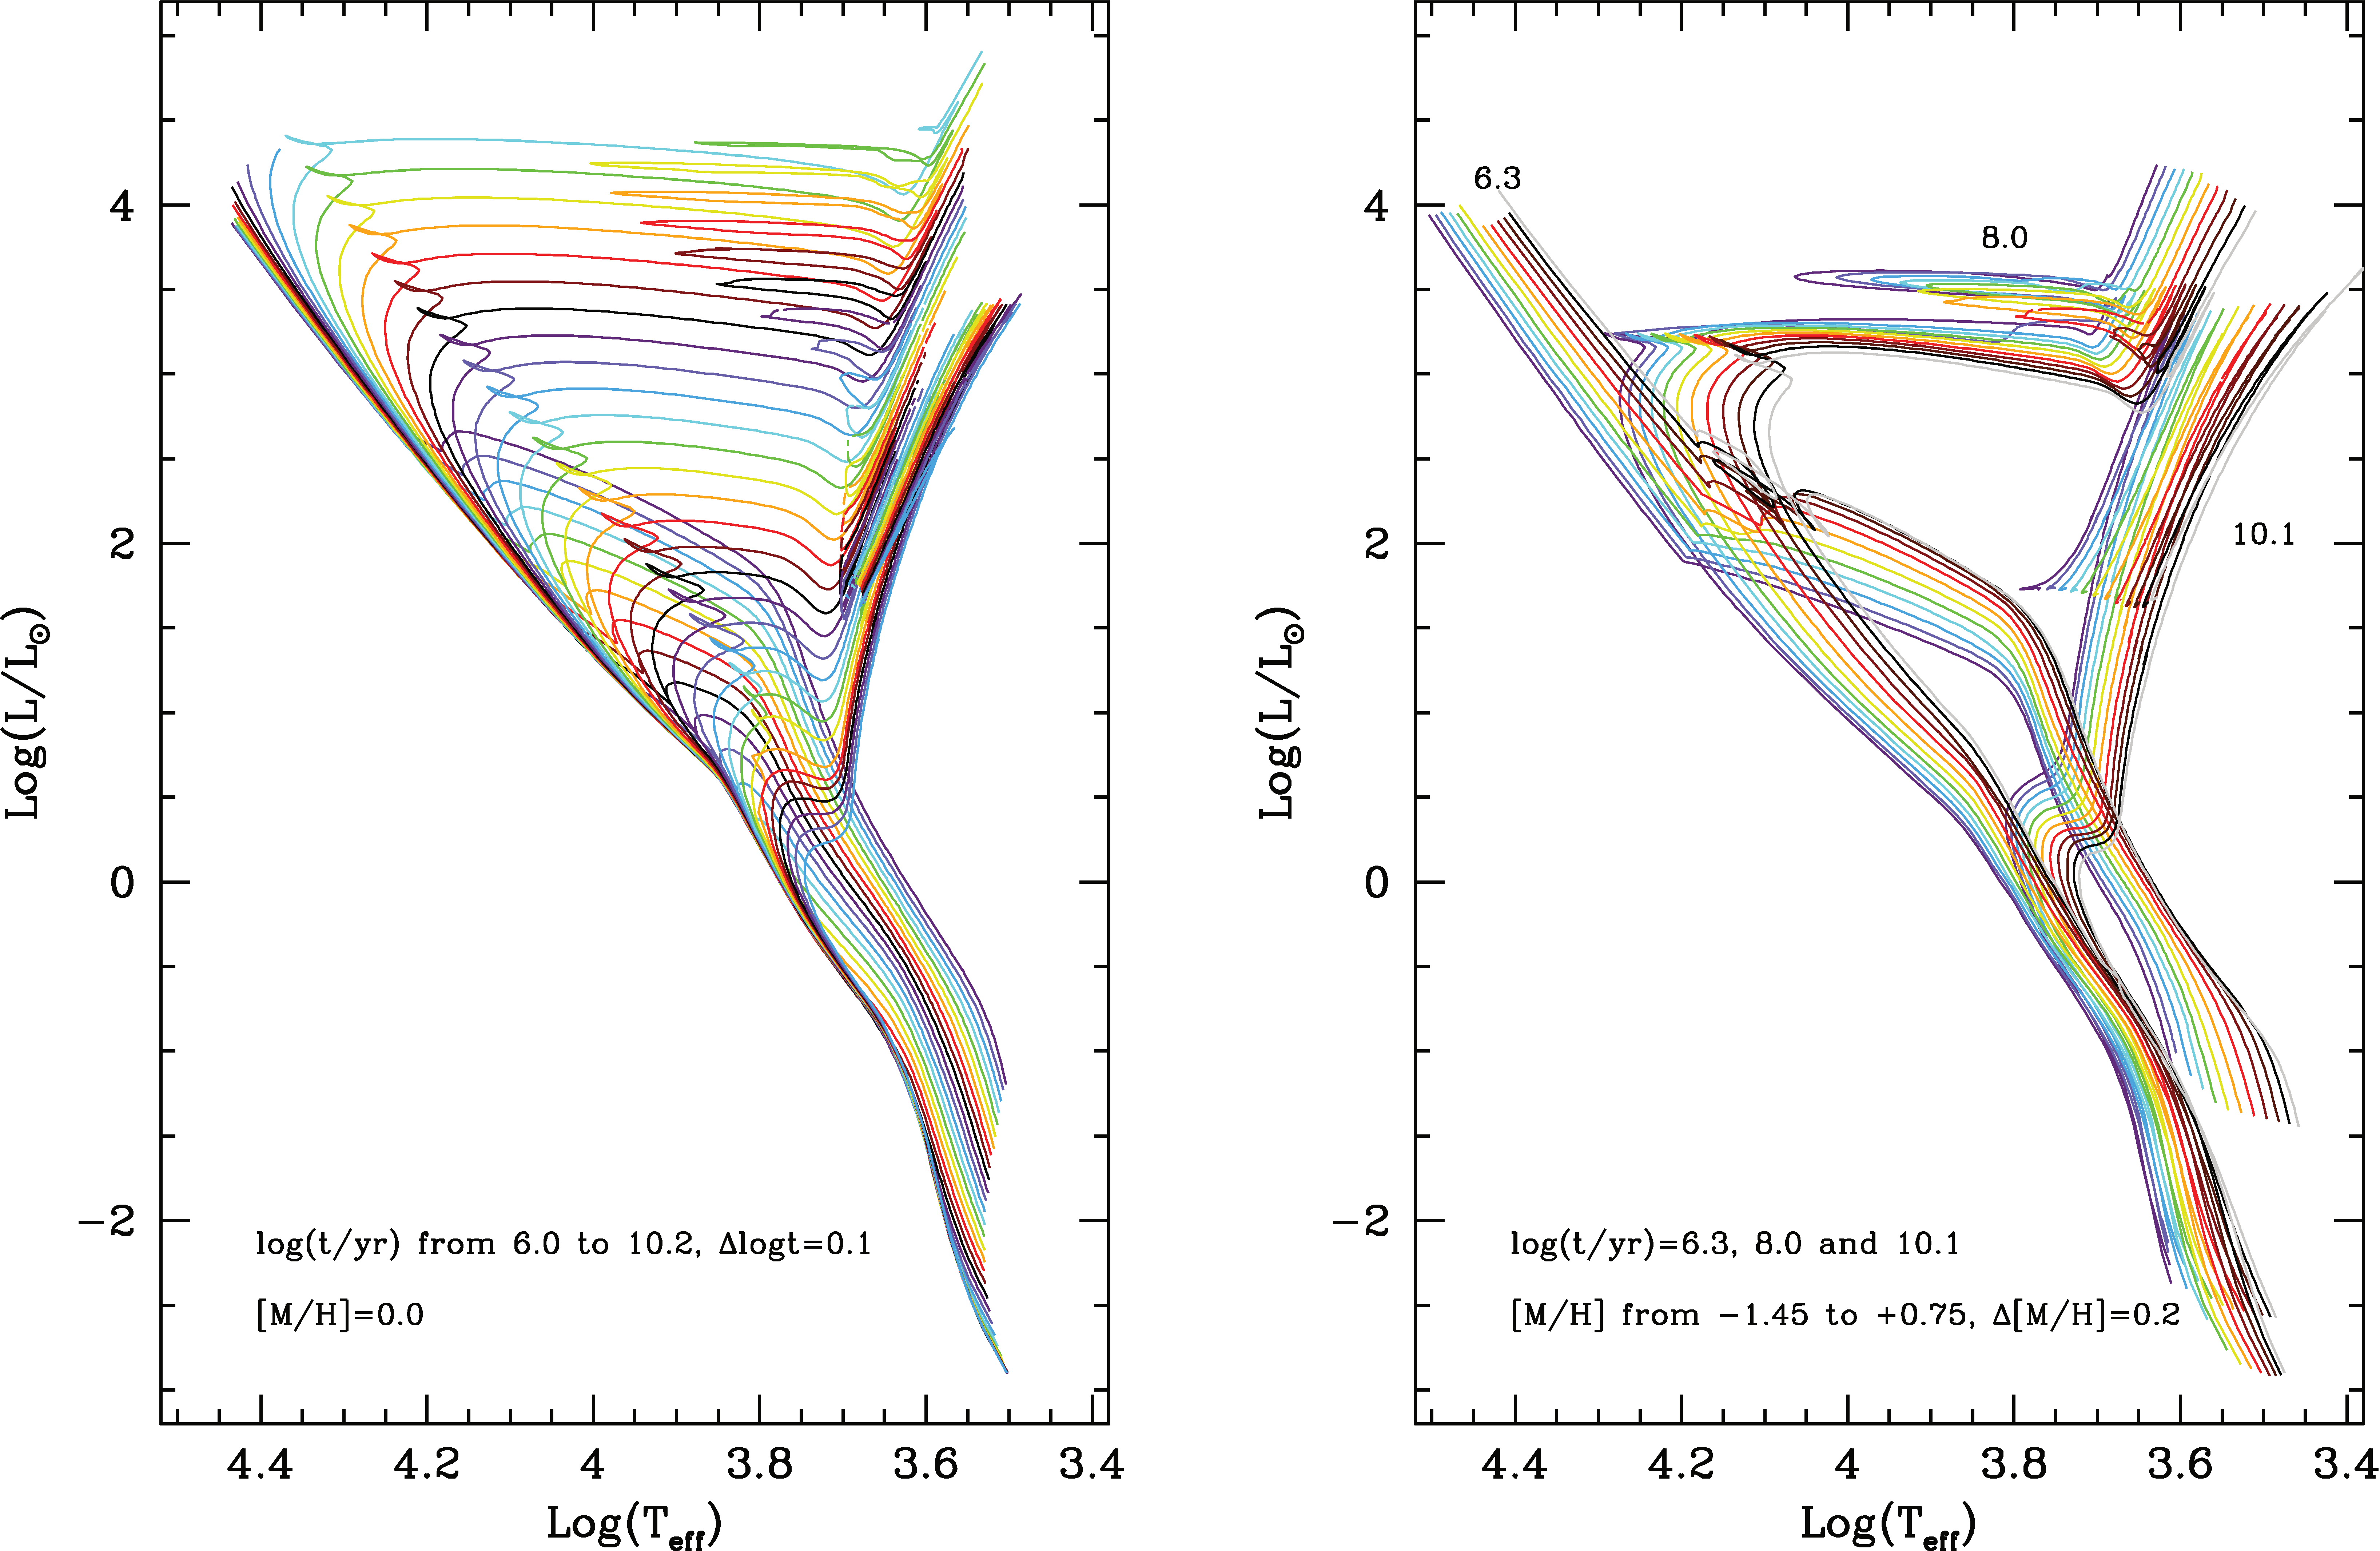
\includegraphics[width=0.9\textwidth]{../figures/theoretical_isochrones_in_hr_diagrams.pdf}
  \caption{Examples of theoretical isochrones in the H-R diagram taken from \protect\citeA[p.~16]{bressan2012parsec}}
  \label{fig:examples_of_isochrones}
\end{figure}

Since these stars were born close in time, they should have a sharp and well-defined profile,
with low scattering through the main sequence in the H-R diagram.
Examples for this kind of diagrams are presented in Figure~\ref{fig:examples_of_hr_diagrams}.

\begin{figure}[htbp]
  \centering
  \begin{subfigure}{0.9\textwidth}
    \centering
    \begin{subfigure}[t]{0.45\textwidth}
      \centering
      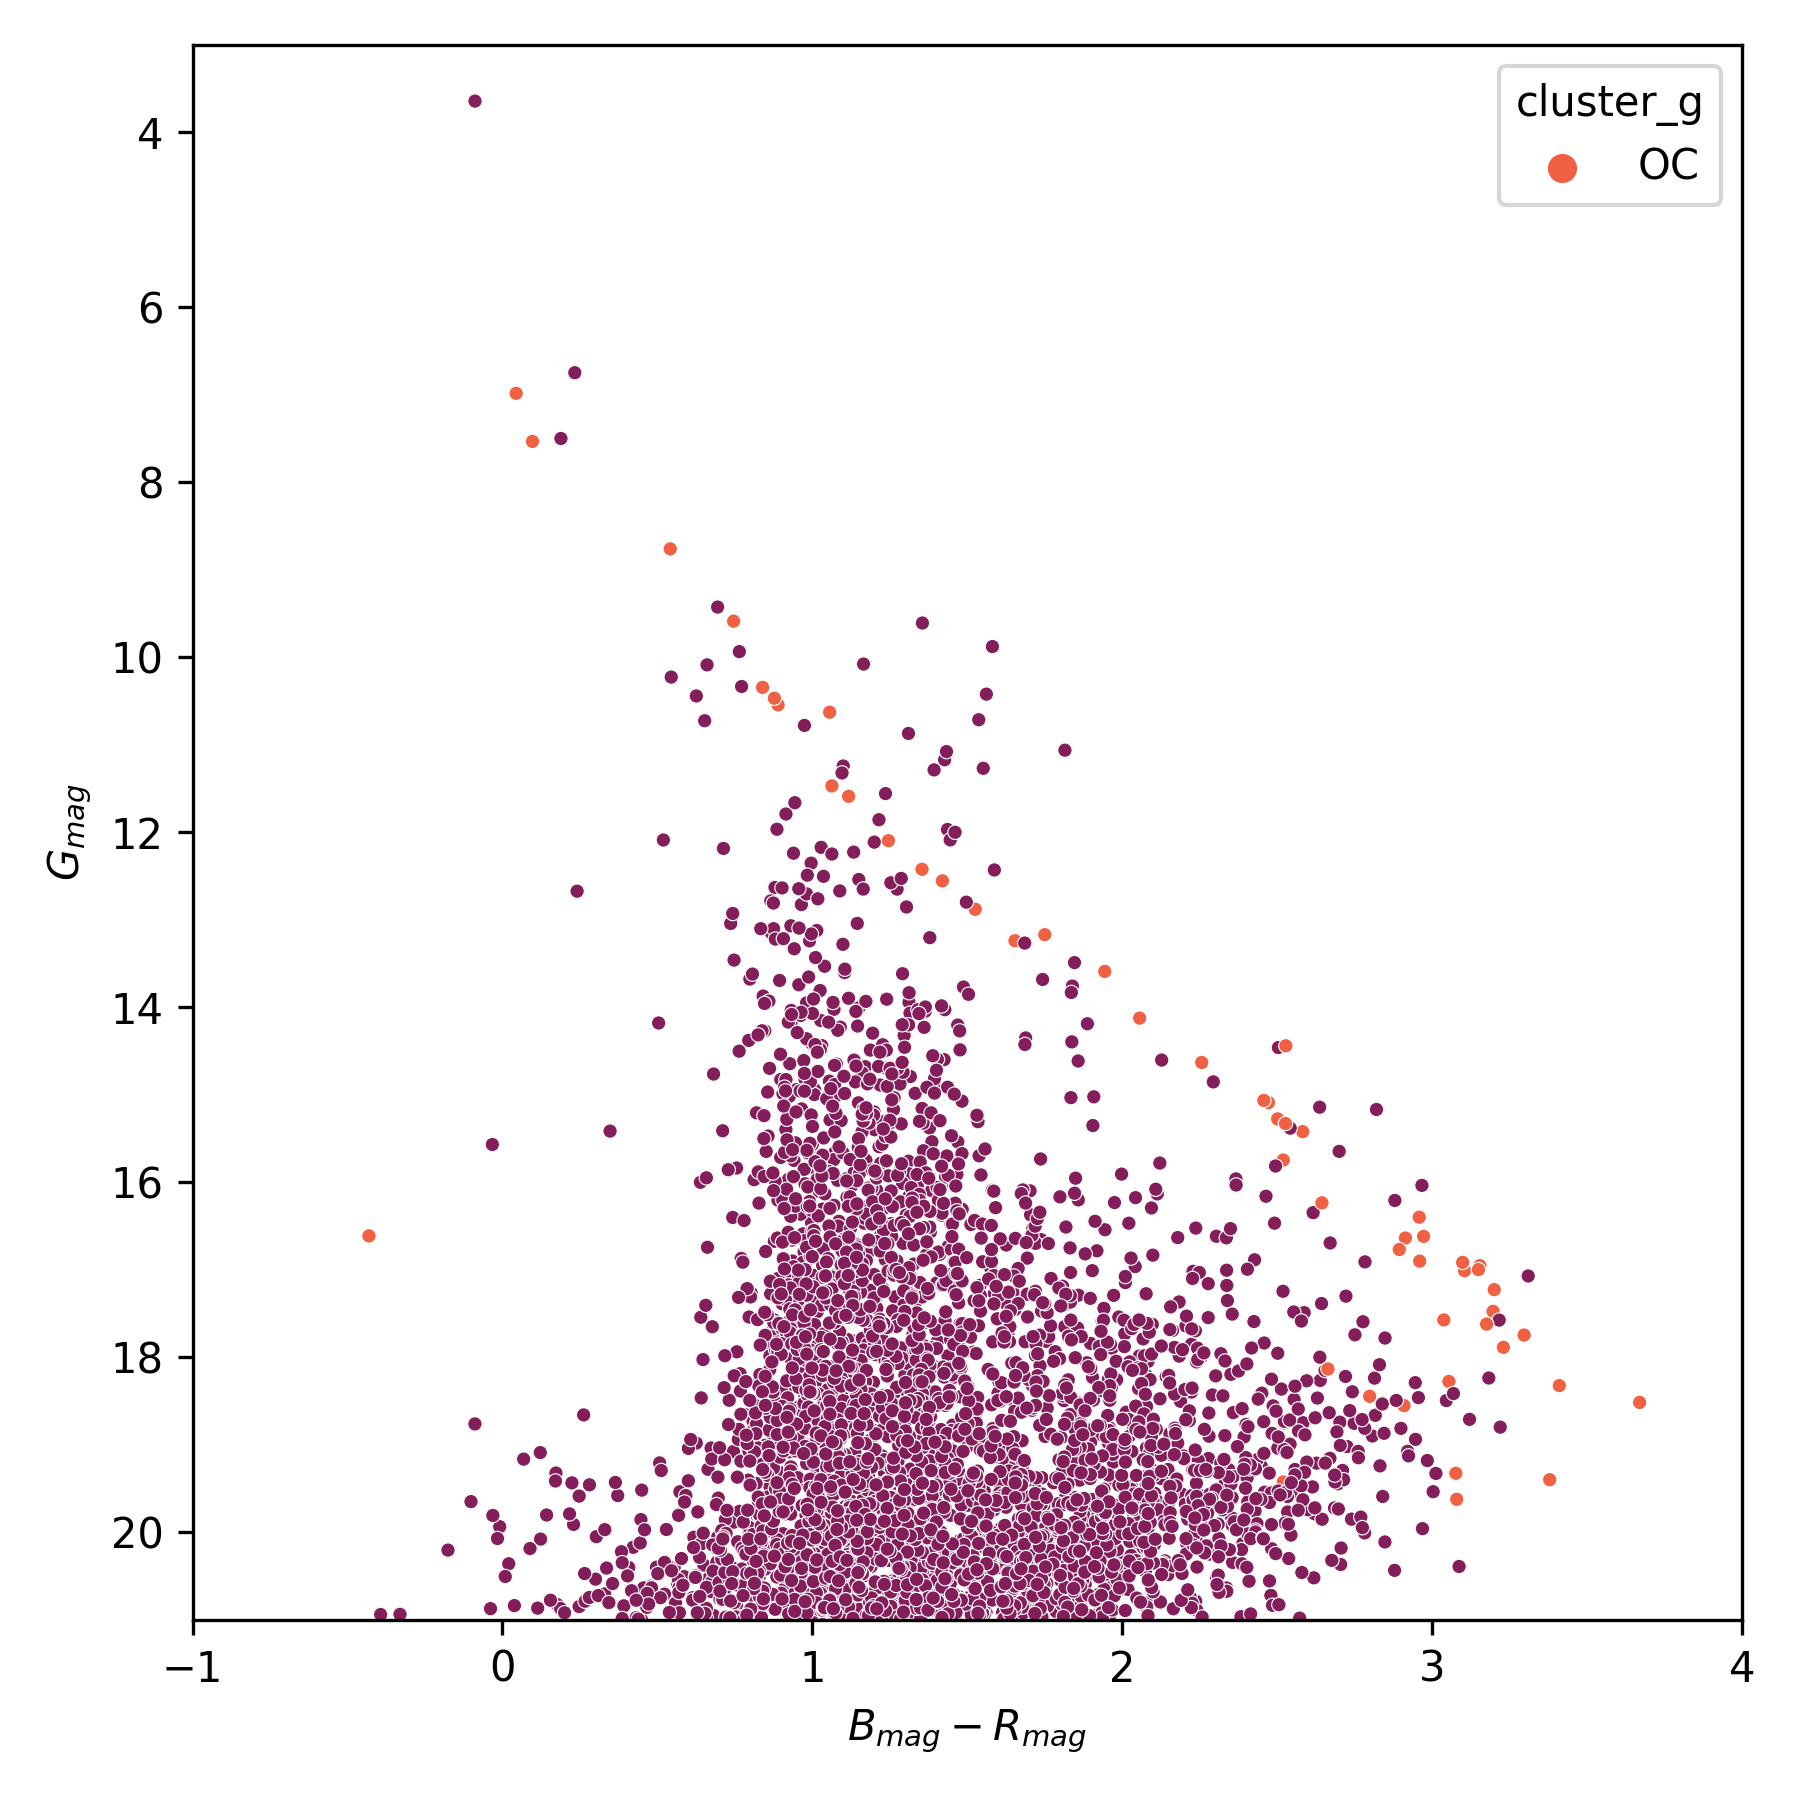
\includegraphics[width=\textwidth]{../figures/melotte_22/hr_diagram_melotte_22.png}
    \end{subfigure}
    \hfill
    \begin{subfigure}[t]{0.45\textwidth}
      \centering
      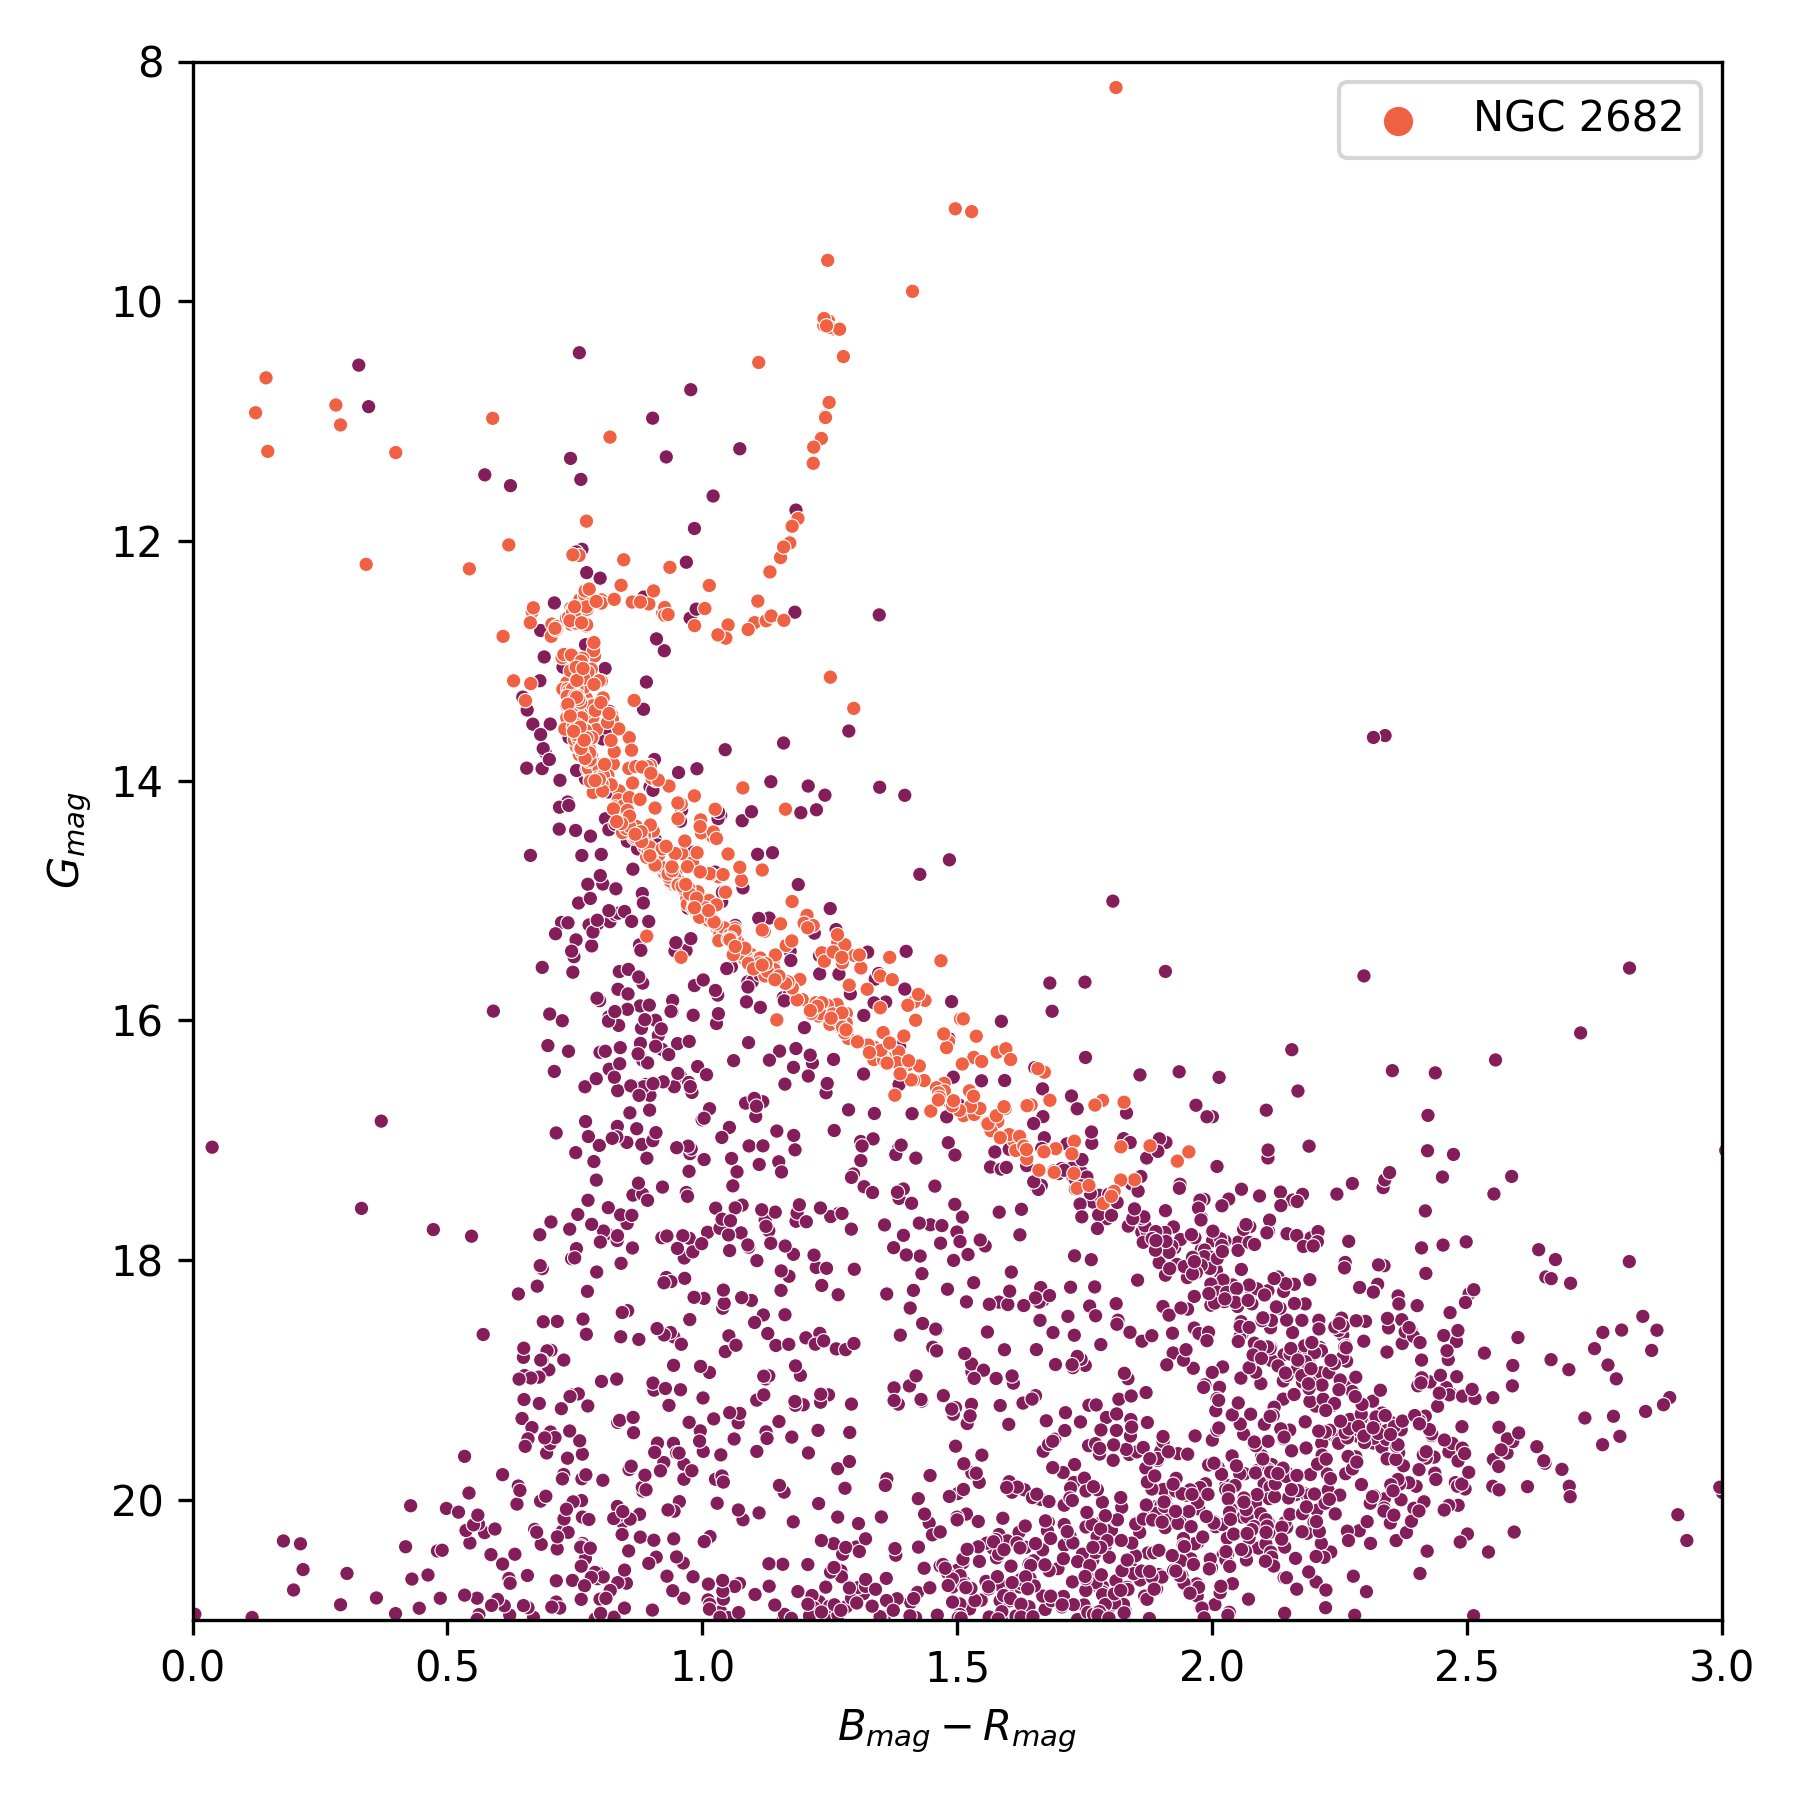
\includegraphics[width=\textwidth]{../figures/ngc_2682/hr_diagram_ngc_2682.png}
    \end{subfigure}
  \end{subfigure}
  \caption{Examples of typical profiles in H-R diagrams for members of open clusters. On the left Melotte 22, on the right NGC 2682.}
  \label{fig:examples_of_hr_diagrams}
\end{figure}

We will take advantage of these properties only to validate our characterization of OCs,
but not to determine what stars belong to them. As we will explain later,
we will only use dynamic properties such as proper motion and parallax to characterize open clusters.

Although the members of a cluster appear in the observational visual field as an overdensity in positions,
as shown in Figure~\ref{fig:pos_ngc_2682},
these coordinates are not useful to separate those stars that belong to the cluster from the other that do not.
However, if we look for overdensities in the proper motion configuration spaces, it is possible, at least at first instance,
to assume a possible membership cut (see Figure~\ref{fig:pm_ngc_2682}.

\begin{figure}[htbp]
  \centering
  \begin{subfigure}{0.9\textwidth}
    \centering
    \begin{subfigure}[t]{0.45\textwidth}
      \centering
      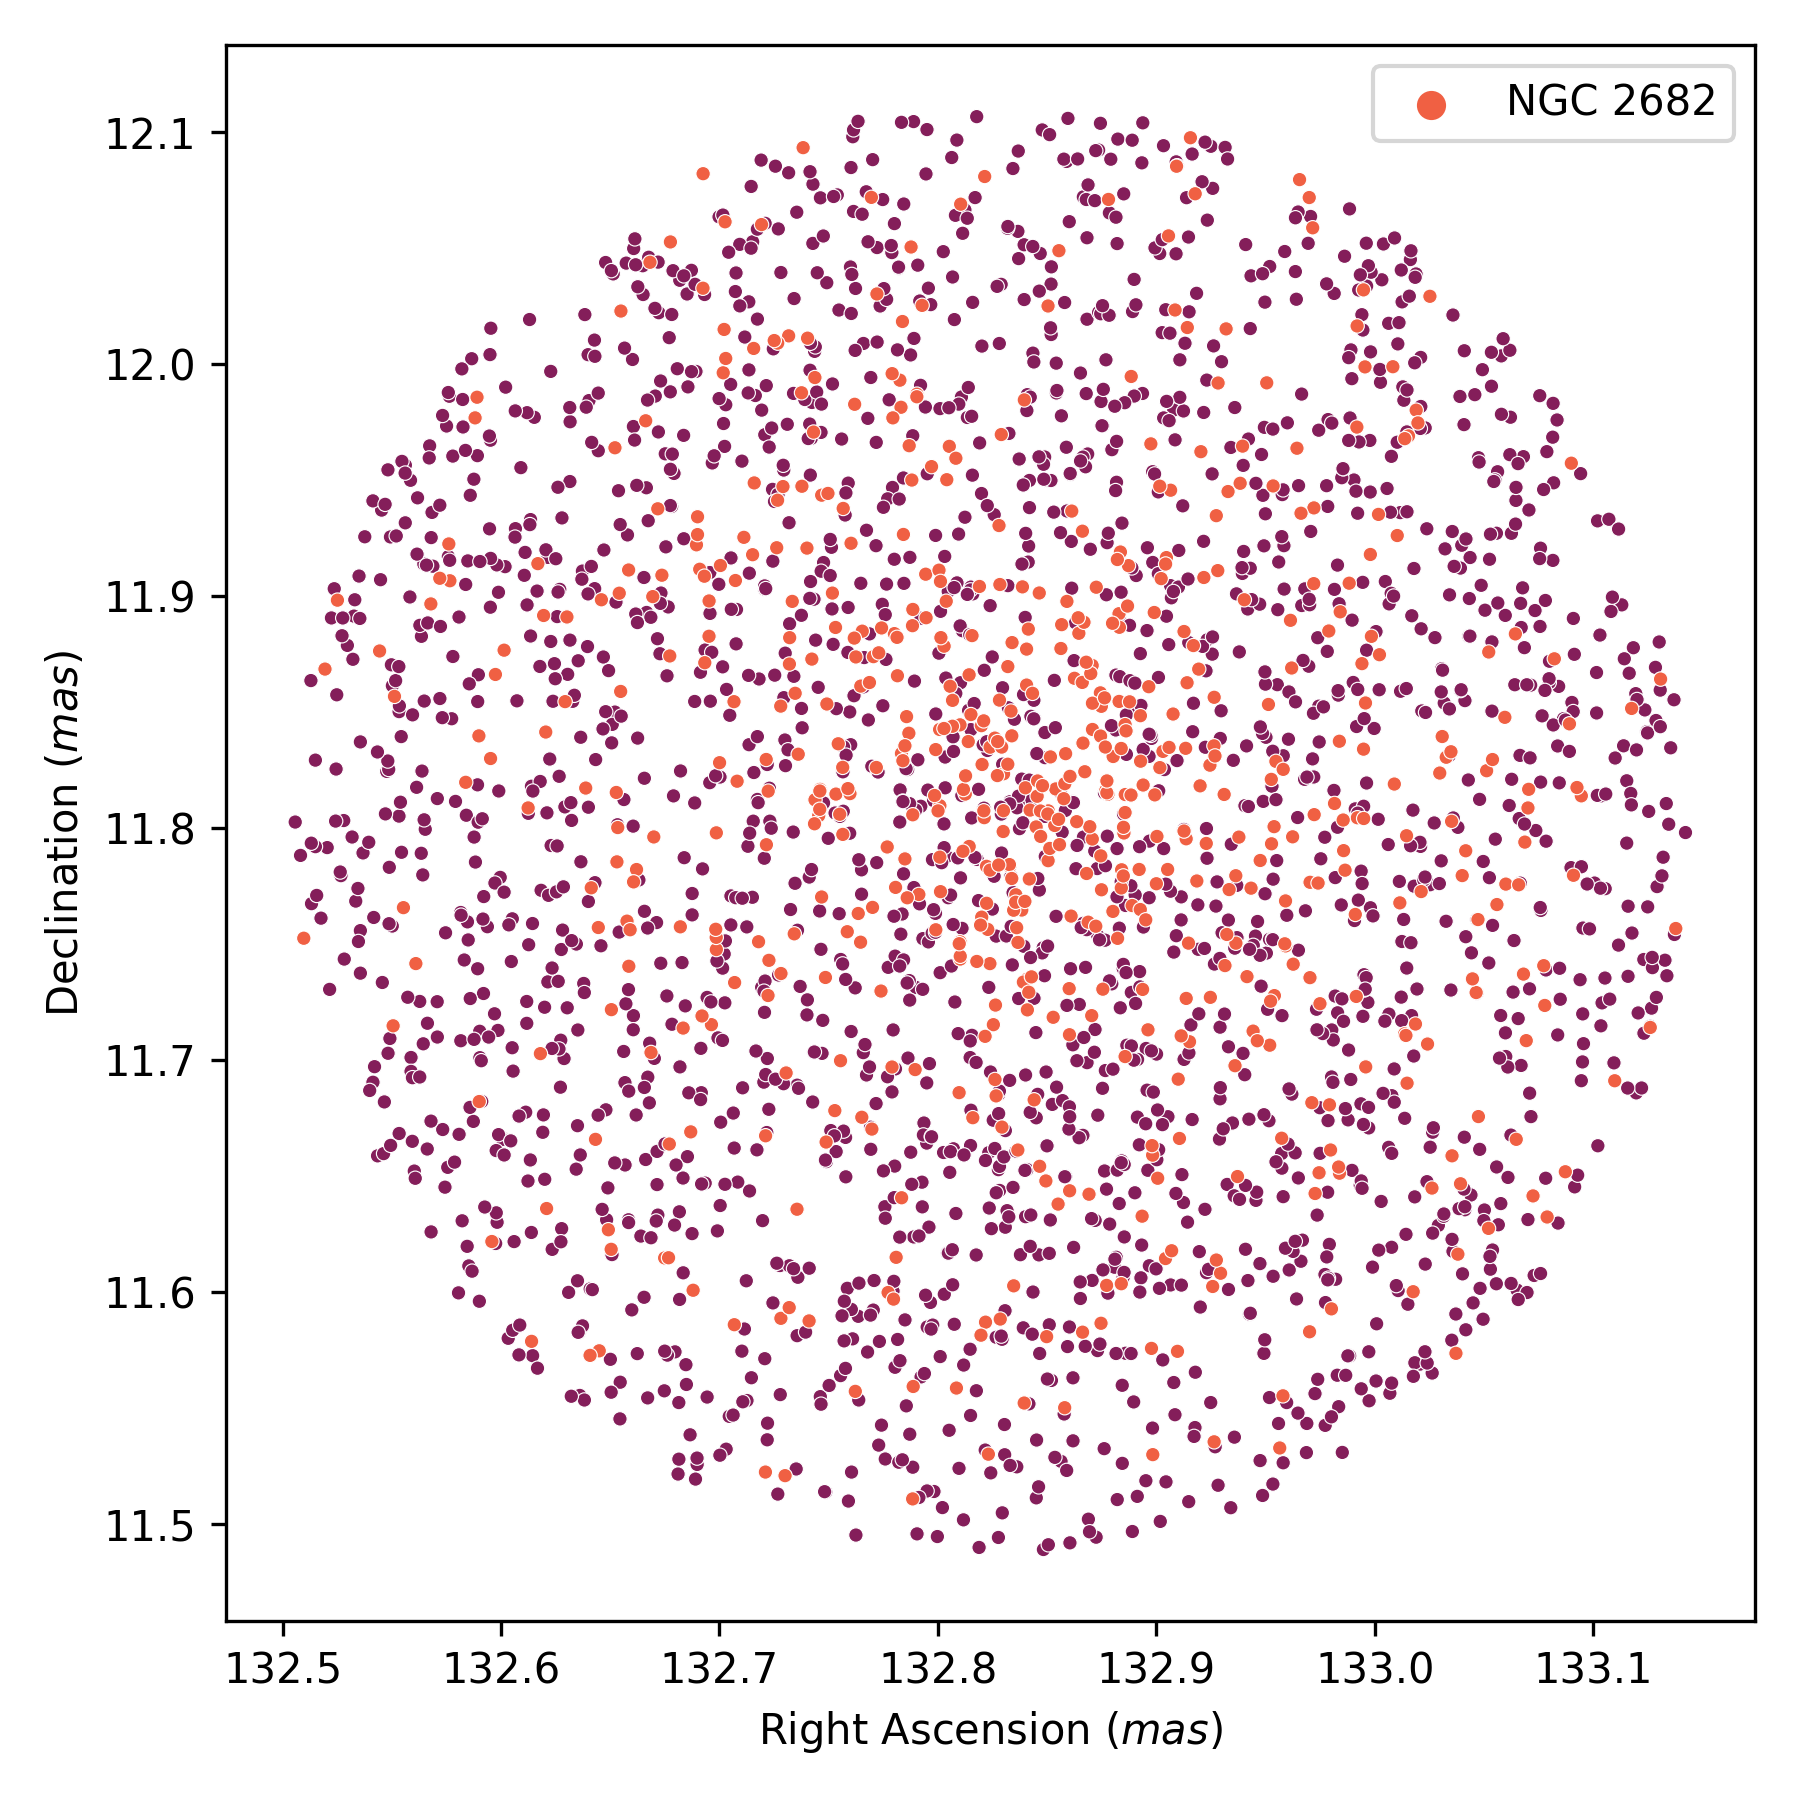
\includegraphics[width=\textwidth]{../figures/ngc_2682/pos_ngc_2682.png}
      \caption{Positions map}
      \label{fig:pos_ngc_2682}
    \end{subfigure}
    \hfill
    \begin{subfigure}[t]{0.45\textwidth}
      \centering
      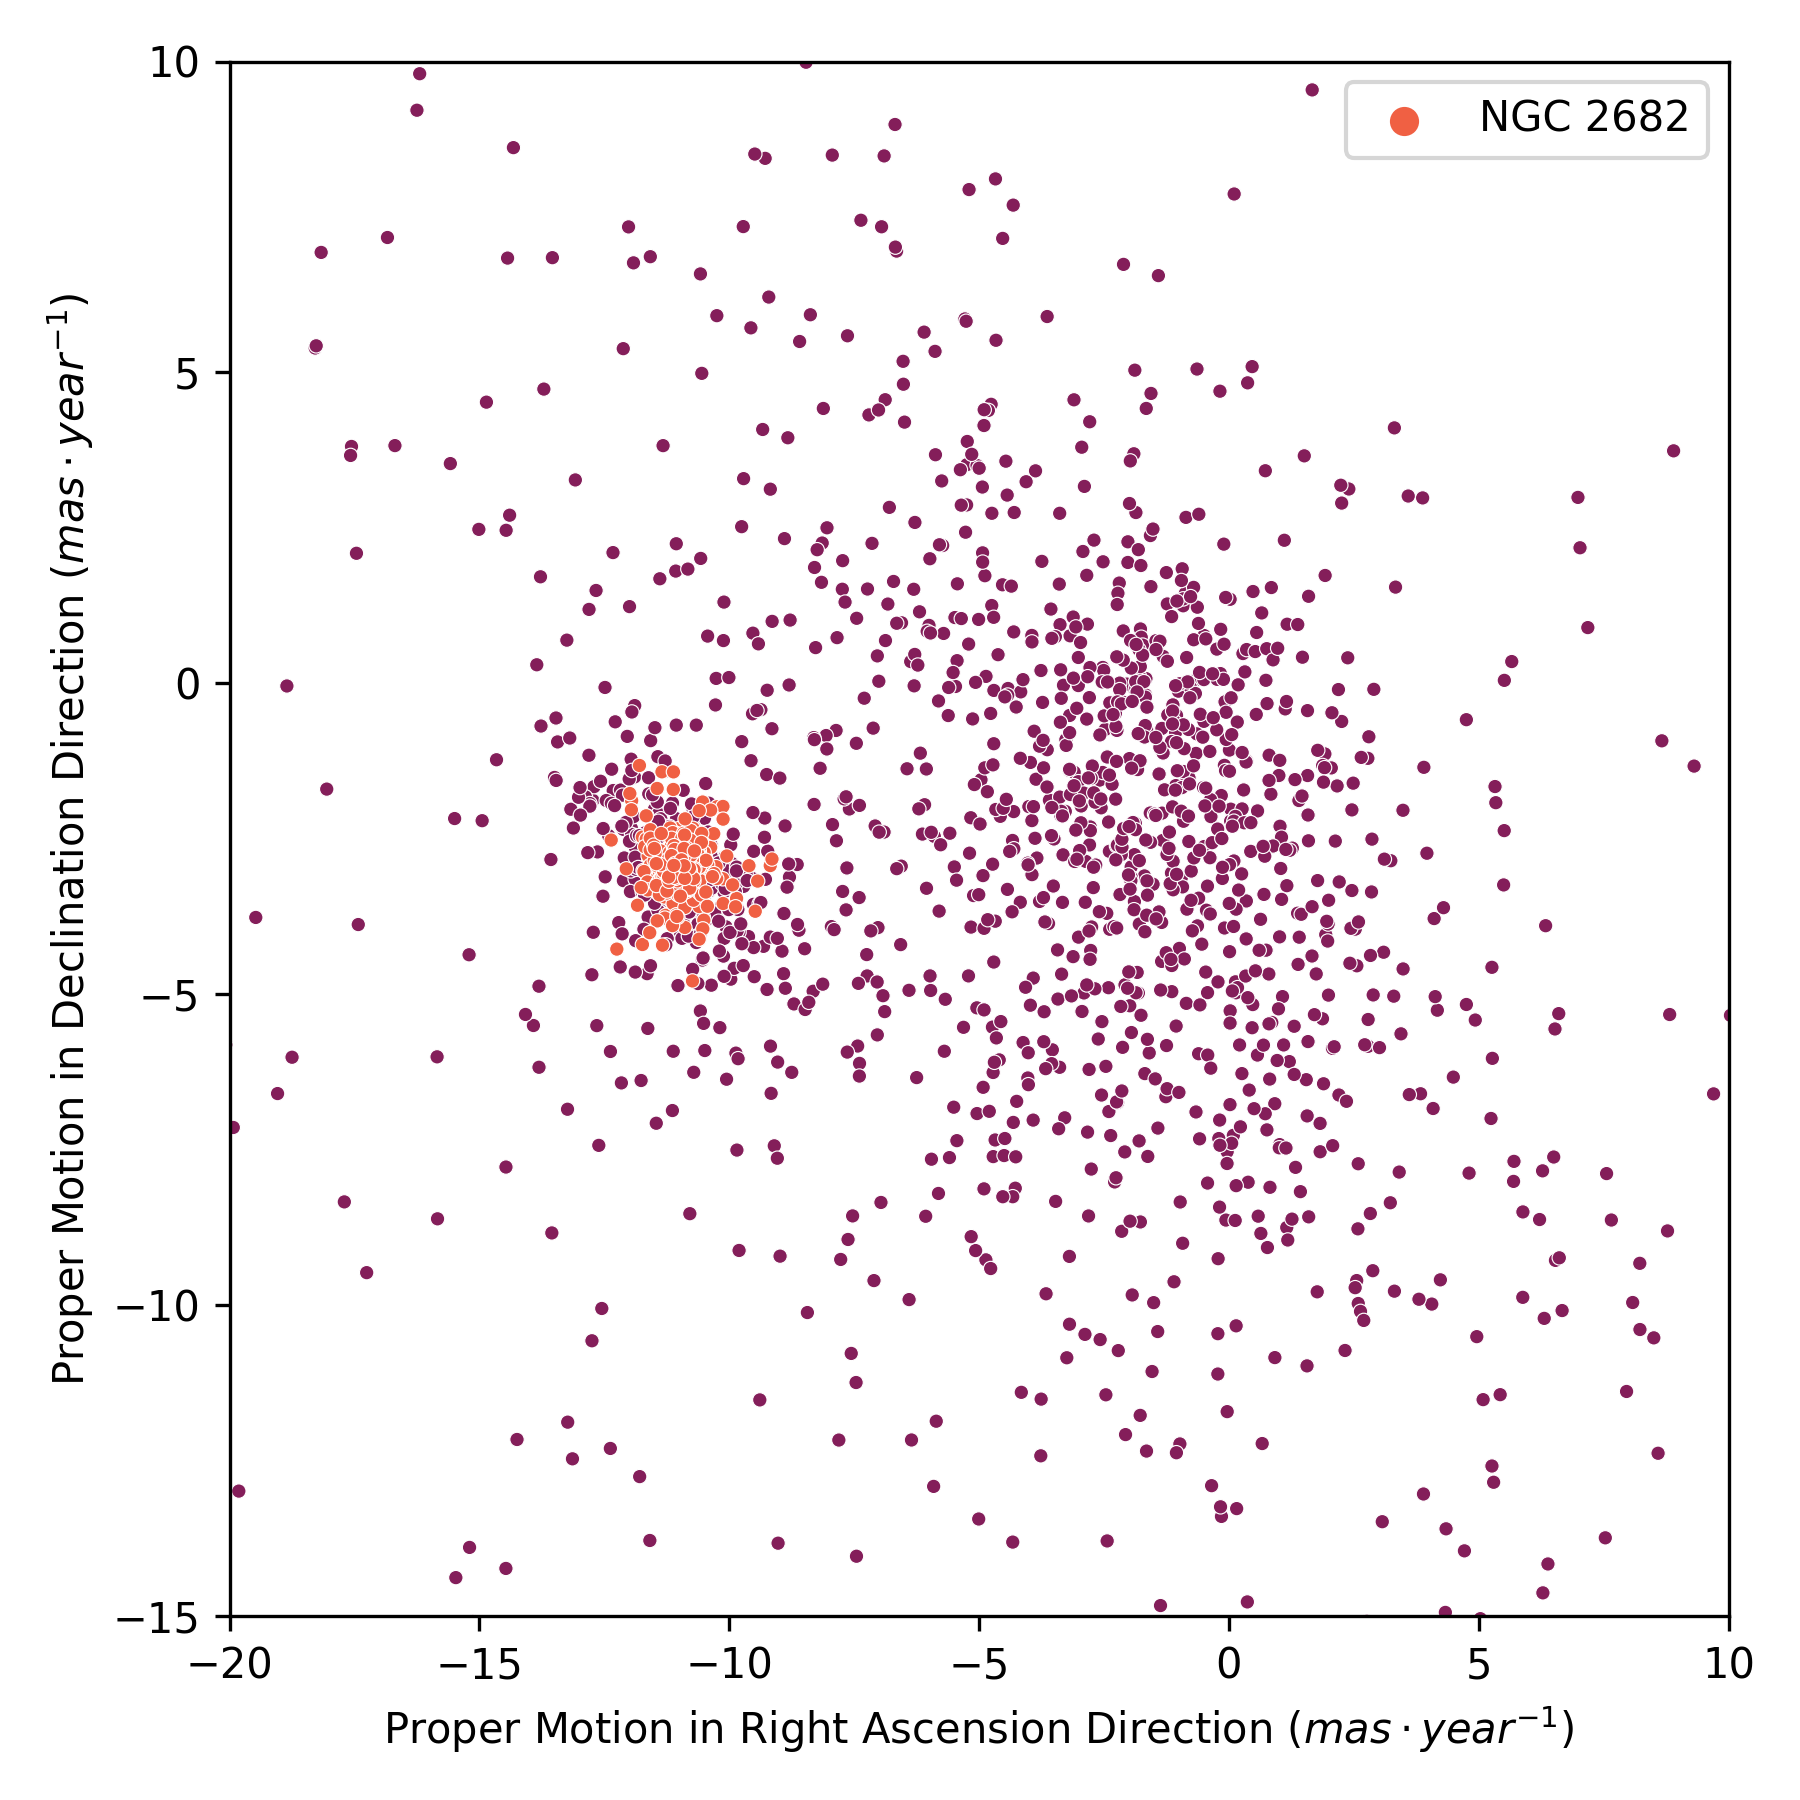
\includegraphics[width=\textwidth]{../figures/ngc_2682/pm_ngc_2682.png}
      \caption{Proper motions}
      \label{fig:pm_ngc_2682}
    \end{subfigure}
  \end{subfigure}
  \caption{NGC 2682 configuration spaces.}
\end{figure}

Overdensities in proper motion are not always so evident.
In order to improve the characterization capabilities of our model,
we will consider the parallax distribution as well.

\begin{figure}[htbp]
  \centering
  \begin{subfigure}{0.9\textwidth}
    \centering
    \begin{subfigure}[t]{0.45\textwidth}
      \centering
      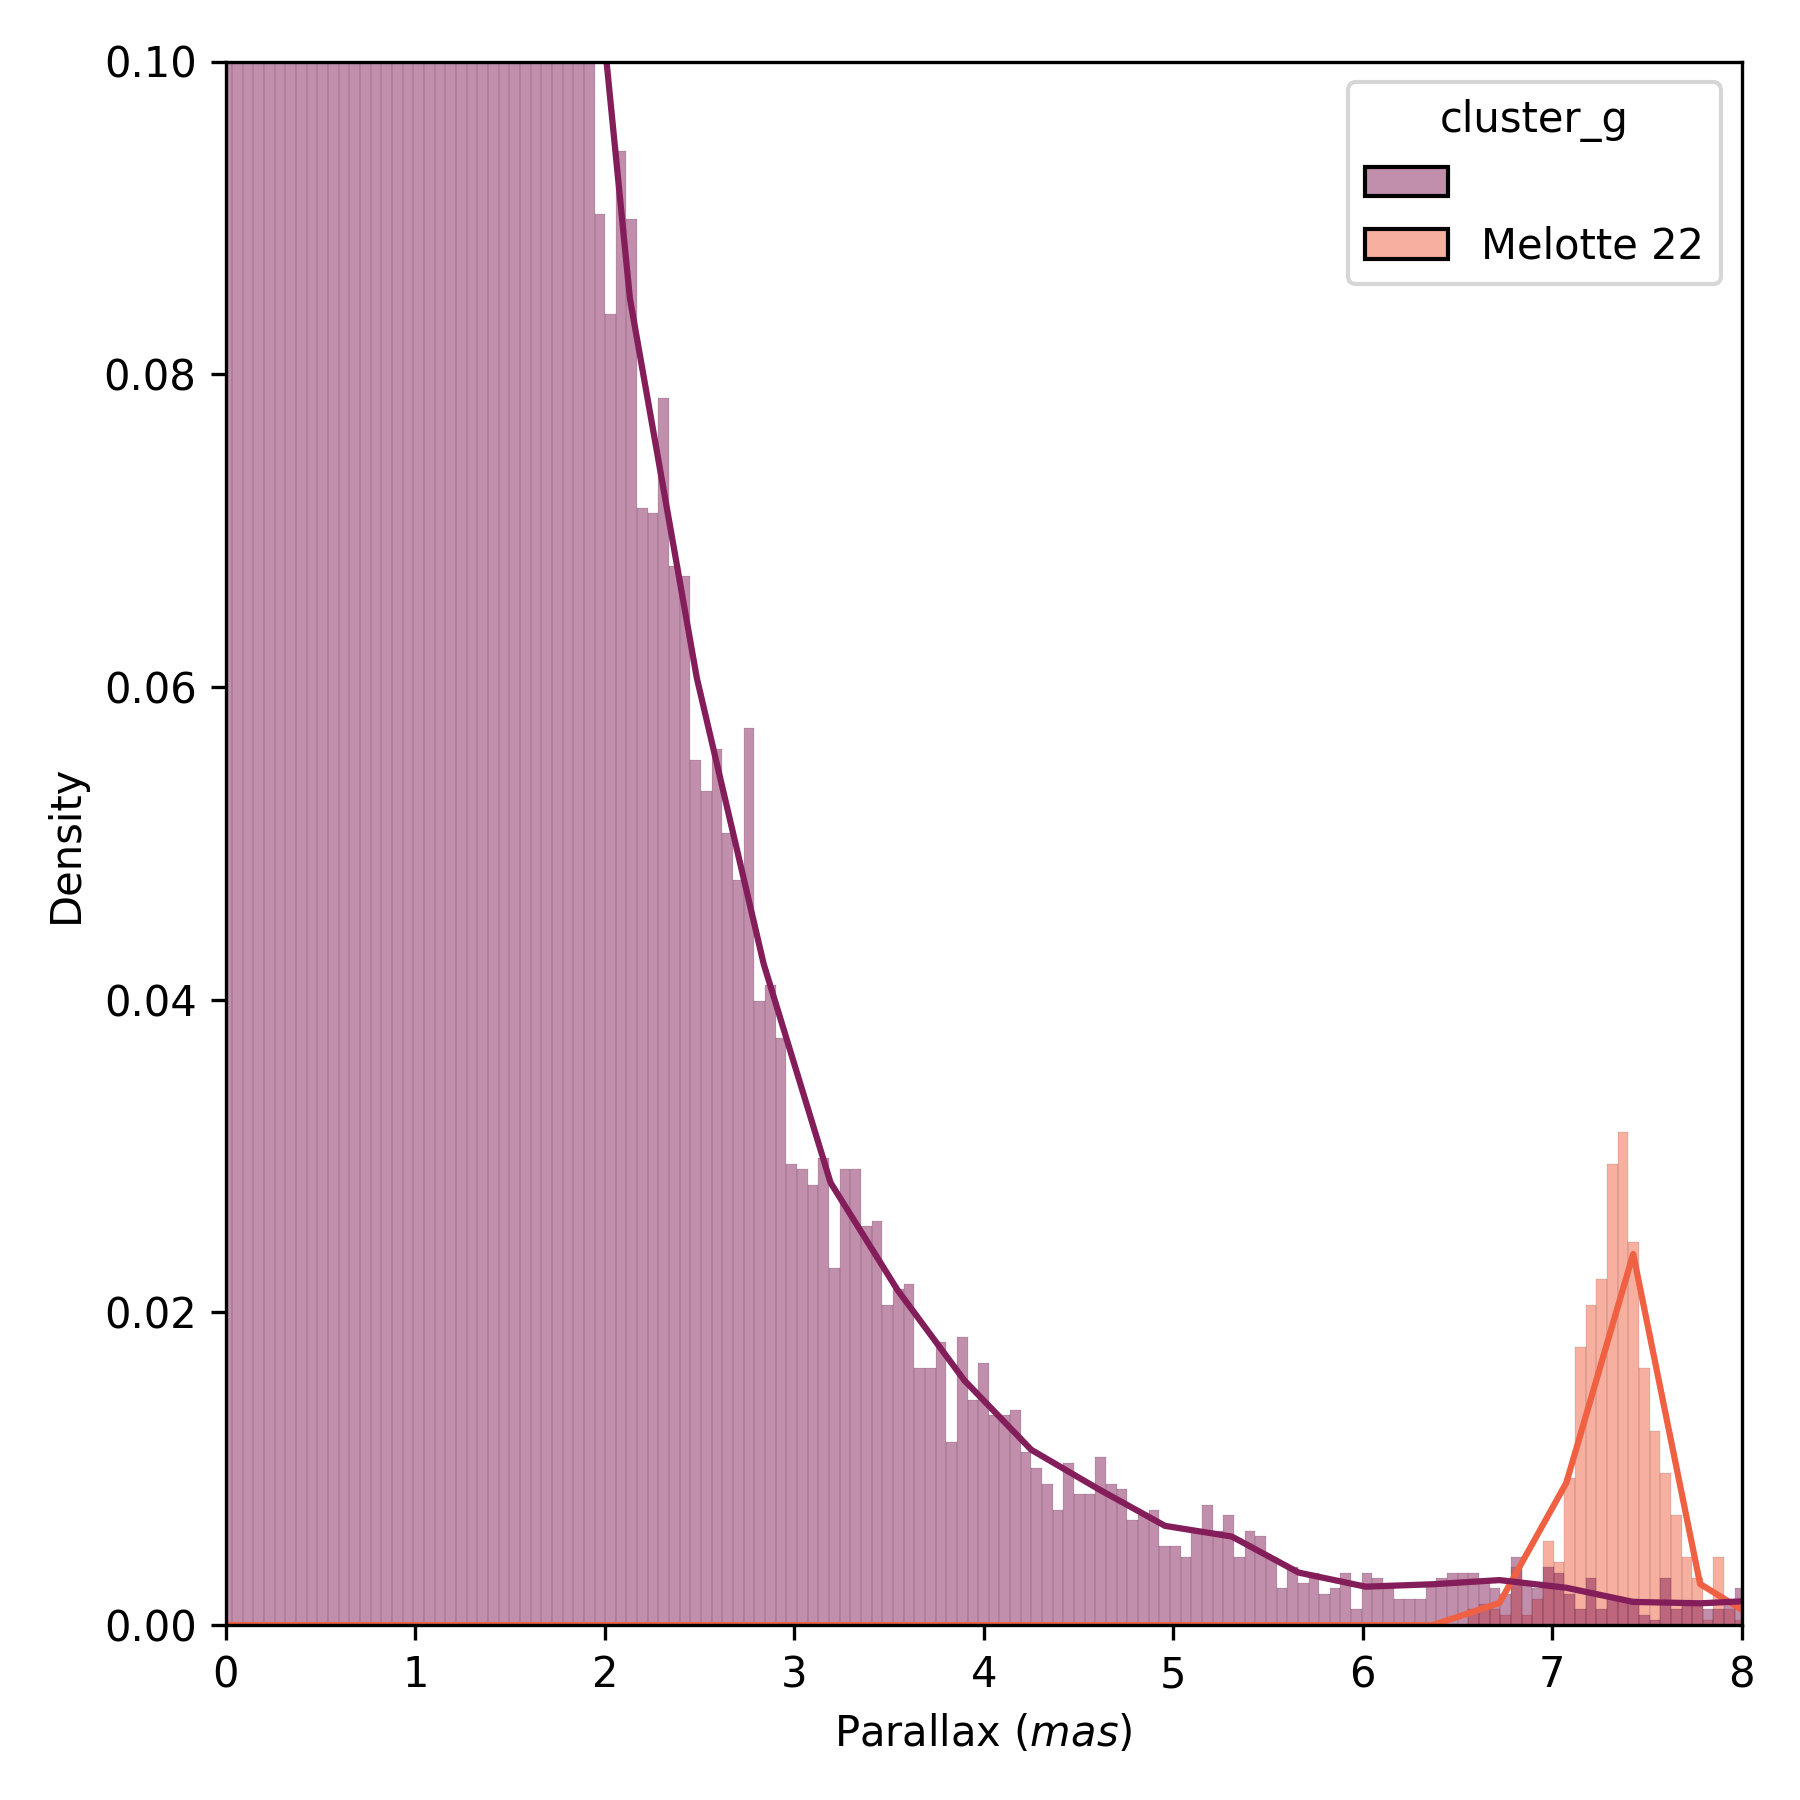
\includegraphics[width=\textwidth]{../figures/melotte_22/parallax_zoom_melotte_22.png}
      \caption{Melotte 22 Parallax}
      \label{fig:melotte_22_parallax_zoom}
    \end{subfigure}
    \hfill
    \begin{subfigure}[t]{0.45\textwidth}
      \centering
      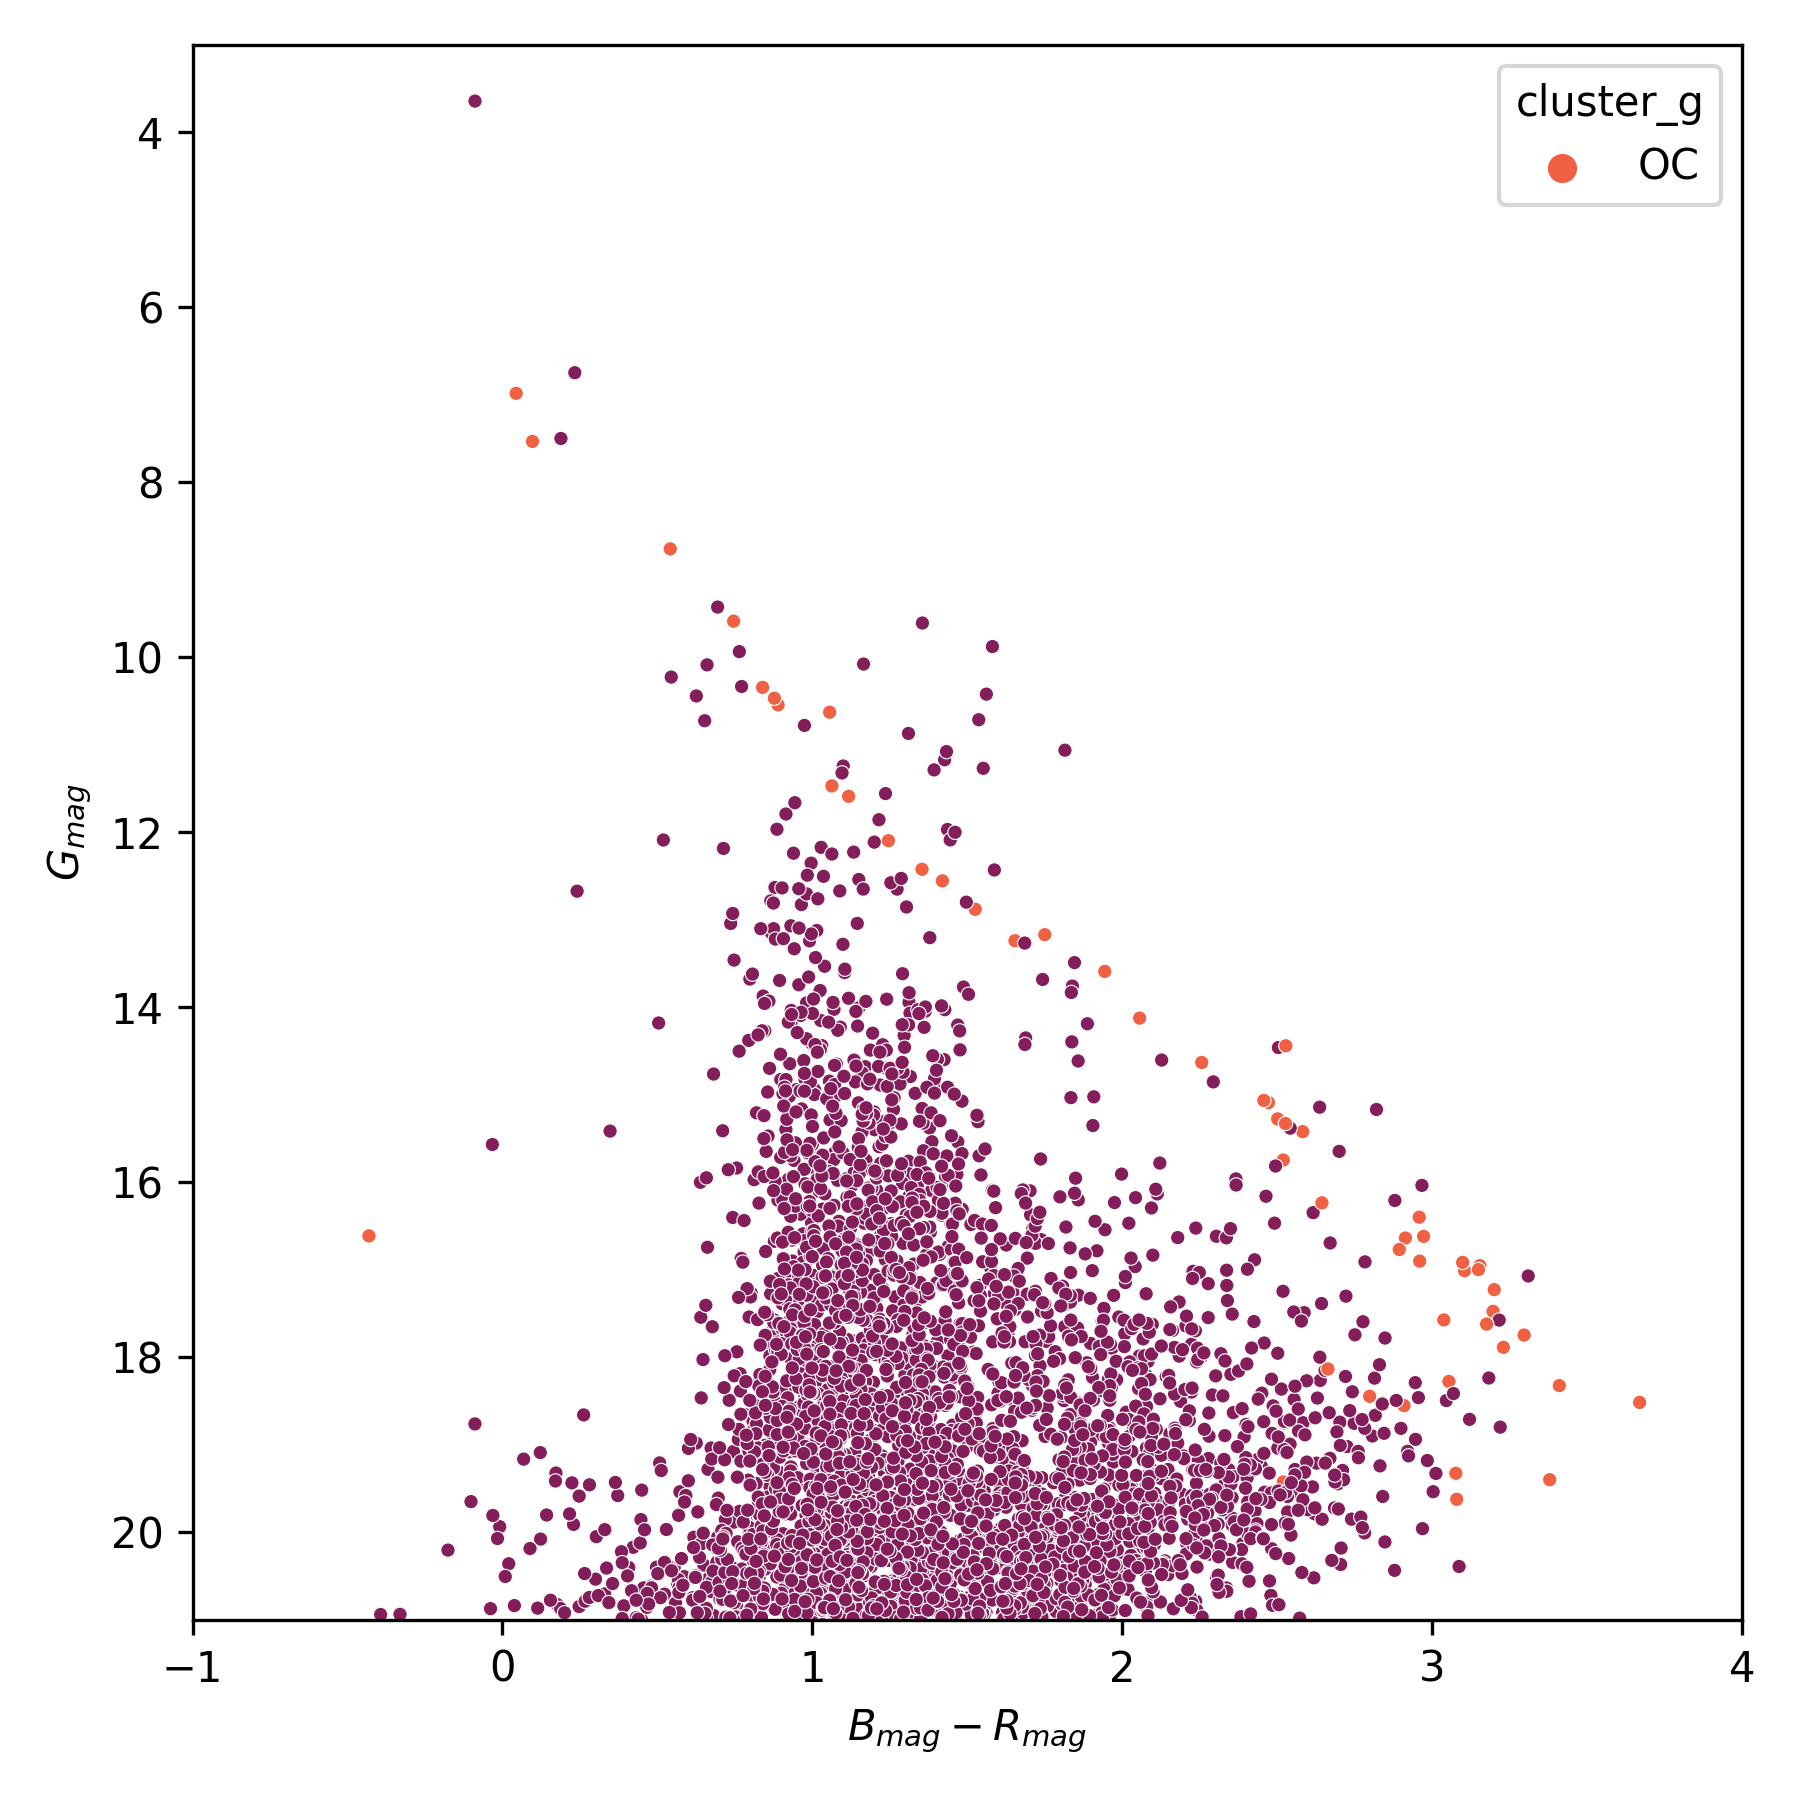
\includegraphics[width=\textwidth]{../figures/melotte_22/hr_diagram_melotte_22.png}
      \caption{Melotte 22 H-R diagram}
    \end{subfigure}
  \end{subfigure}
  \caption{Melotte 22 Parallax histogram, clearly differentiated around the value $\approx 7.3mas$
           and the corresponding diagram from the photometric magnitudes.}
  \label{fig:melotte_22_pm_parallax}
\end{figure}

In many other cases things are not so simple,
and the characterization process can turn very difficult and tedious using tools such as the available ones at the Virtual Observatory (VO).
Furthermore, it frequently requires a parametrization based on prior knowledge regarding the studied region.
The aim of this work is to test an unsupervised and non-parameterized model based on Machine Learning (ML) tools.

We start by enumerating the aims we try to achieve with this work.
Then, we expose the current \emph{state of the art}, mentioning the \emph{Gaia Mission} used as data source in this work and
describing other related works that try to solve this problem.
The state of the art ends with a brief summary for some of the clustering algorithms available today.
In the \emph{Method} chapter, we explain our model to improve open cluster characterization.
Also, we show an alternative method based on current procedures.
We have used this alternative technique as a validation method to test ours.
Then, a comparison between a set of results obtained with our method and the results obtained
for the same clusters with the validation method is presented.
Finally, we extract some conclusions based on the obtained results and present
further researches that can be done in light of the results.

\chapter{Aims}

\section{General}

The primary aim of this thesis is to \emph{build an unsupervised clustering model for open cluster characterization}.
The model must be \emph{non-supervised and non-parameterized} to fit a wide range of clusters without
the need for fine-tuning a high number of hyperparameters.

\section{Specific}

To achieve the general goal, we will set the following milestones:

\begin{itemize}
  \item Gather information on the \emph{state of the art}.
  \item Research unsupervised clustering algorithms suitable for grouping stars previously recovered.
  \item Recover data from Gaia DR2 database. This data will be taken as source for the machine learning model to characterize open clusters
  by grouping stars into clusters.
  \item Select and implement unsupervised clustering algorithms from the previous study.
  \item Use chosen algorithms with different datasets to find OCs.
  \item Look for an independent technique to use it as a validation method.
  \item Validate OCs found with our custom model by making comparisons with the validation method.
\end{itemize}

\chapter{State of the Art}

An initial approach for finding OCs is the search for overdensities along the galactic disk.
In general, this is a good starting point but, although it seems simple,
it presents a fundamental problem already discussed.
The near field around the OC is filled with two types of distinct star populations:
those who belong to the OC (tens or hundreds to a few thousand)
and a background made up of thousands or millions of stars that are not.
Finding out which stars belong to the first group is the problem faced in this work.
This selection is crucial to properly characterize the fundamental properties of the cluster
(dynamics, total mass, age, chemical composition, among other).

Sometimes, the problem is easy to solve, as we have seen, by studying astrometric parameters
and looking for overdensities in the proper motion configuration space as well as in the parallax space.

\begin{figure}[htbp]
  \centering
  \begin{subfigure}{0.9\textwidth}
    \centering
    \begin{subfigure}[t]{0.45\textwidth}
      \centering
      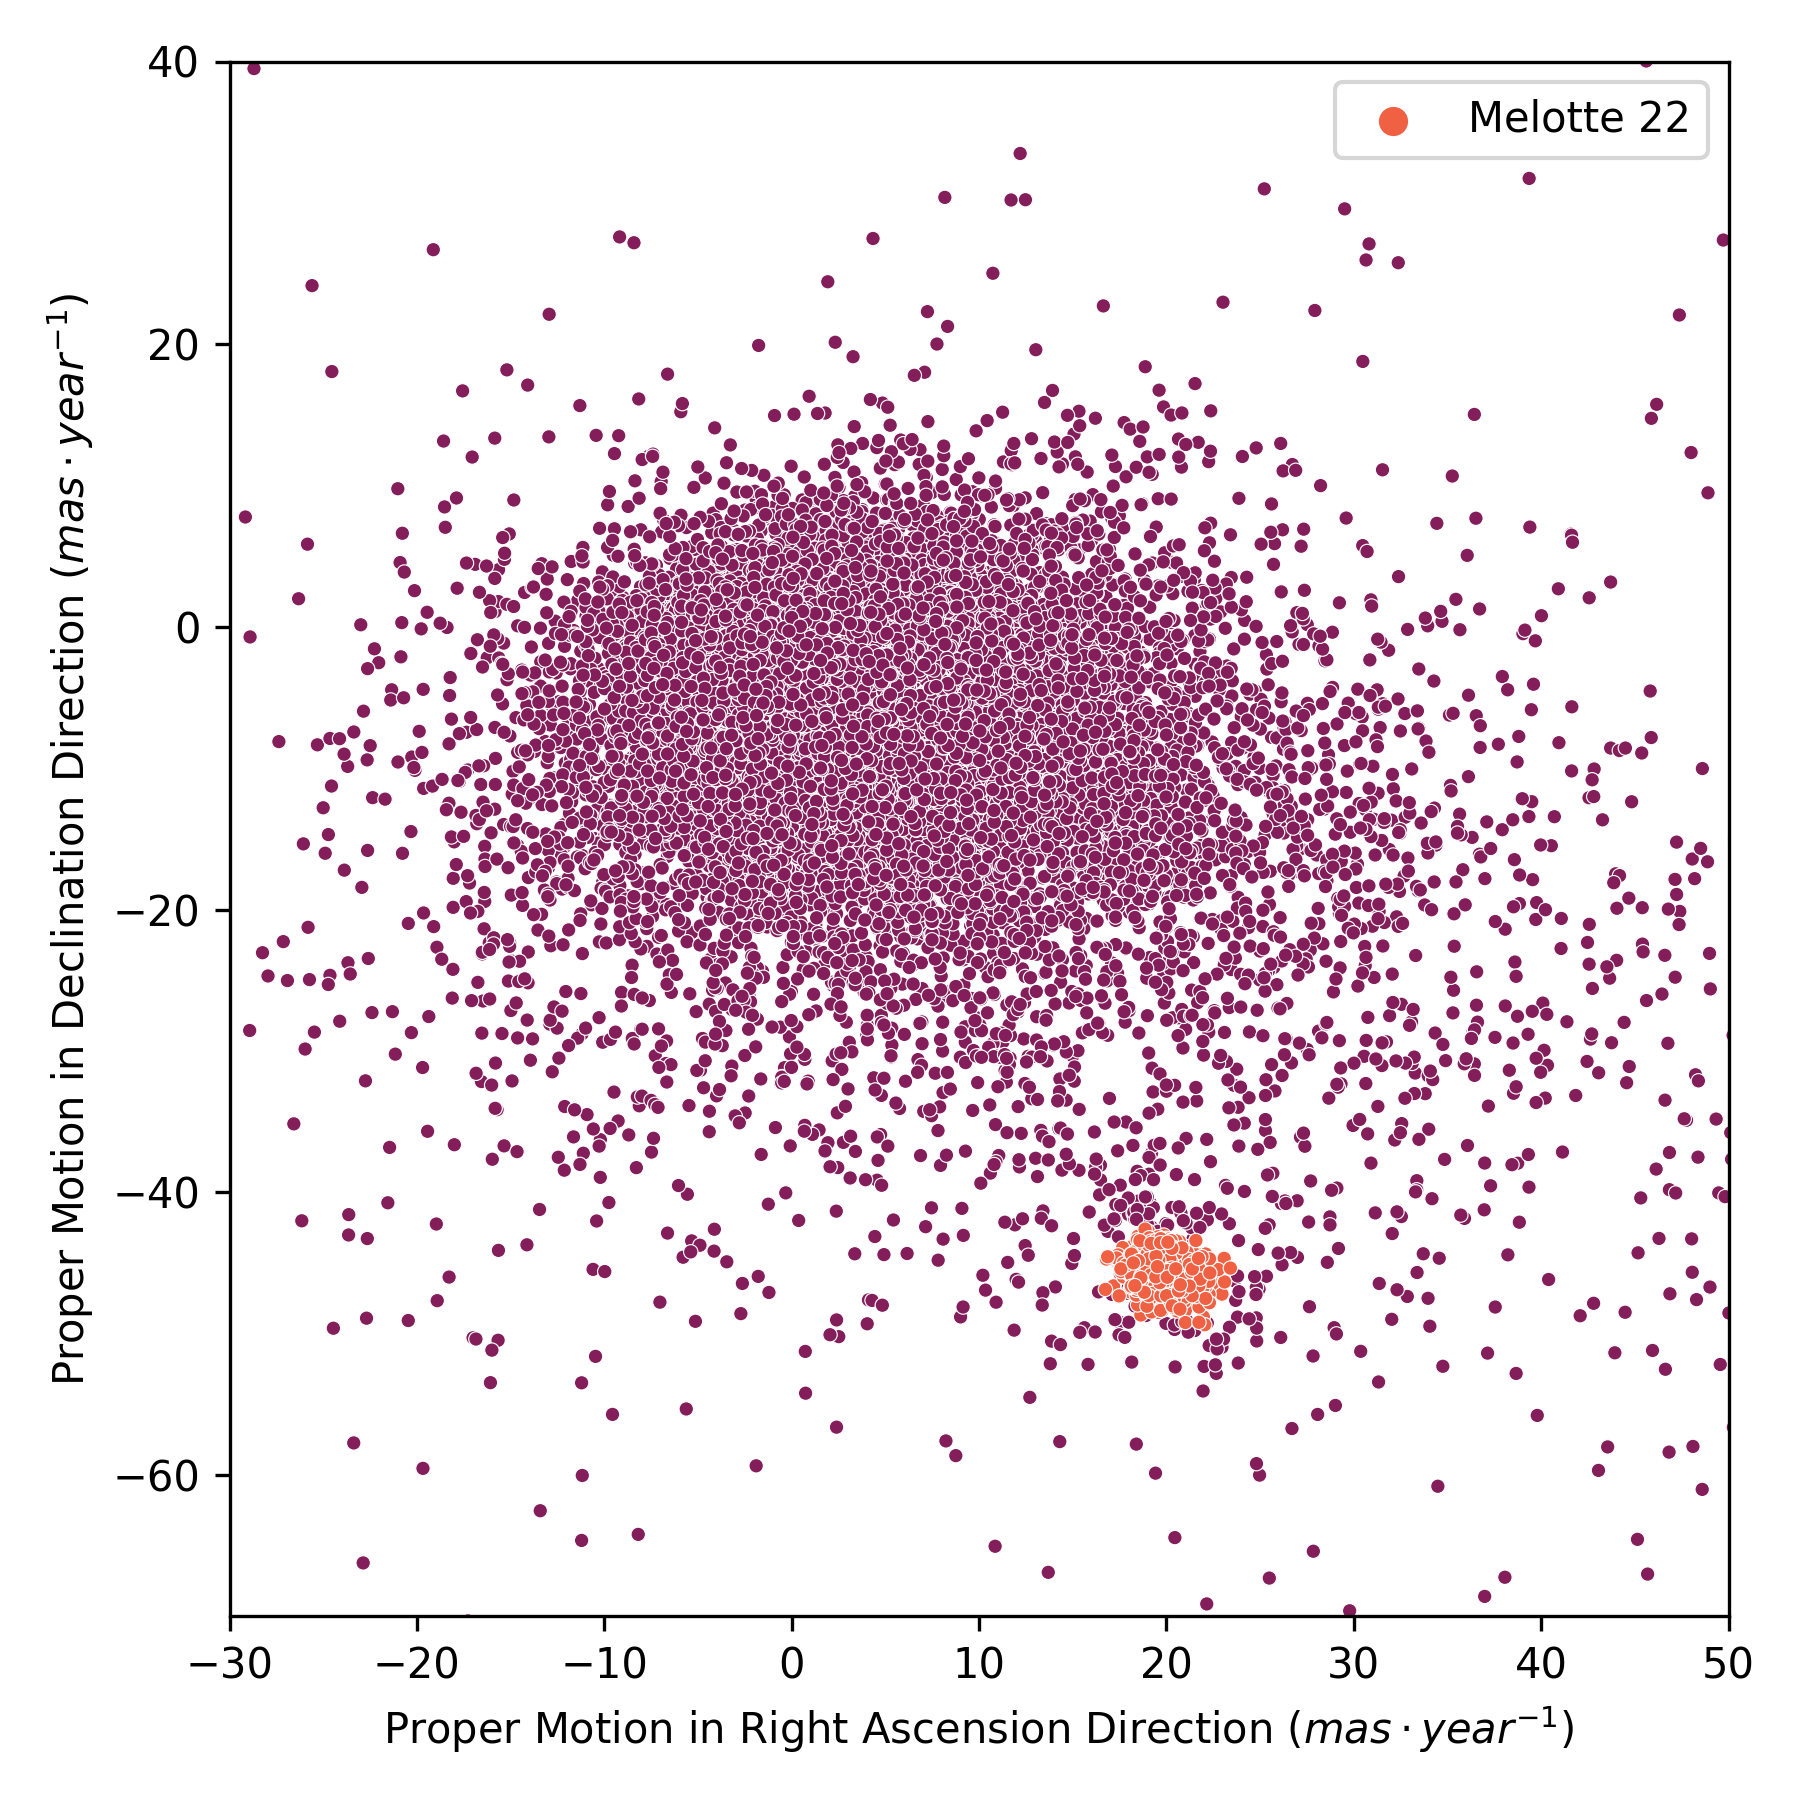
\includegraphics[width=\textwidth]{../figures/melotte_22/pm_melotte_22.png}
      \caption{Proper motions}
      \label{fig:pm_melotte_22}
    \end{subfigure}
    \hfill
    \begin{subfigure}[t]{0.45\textwidth}
      \centering
      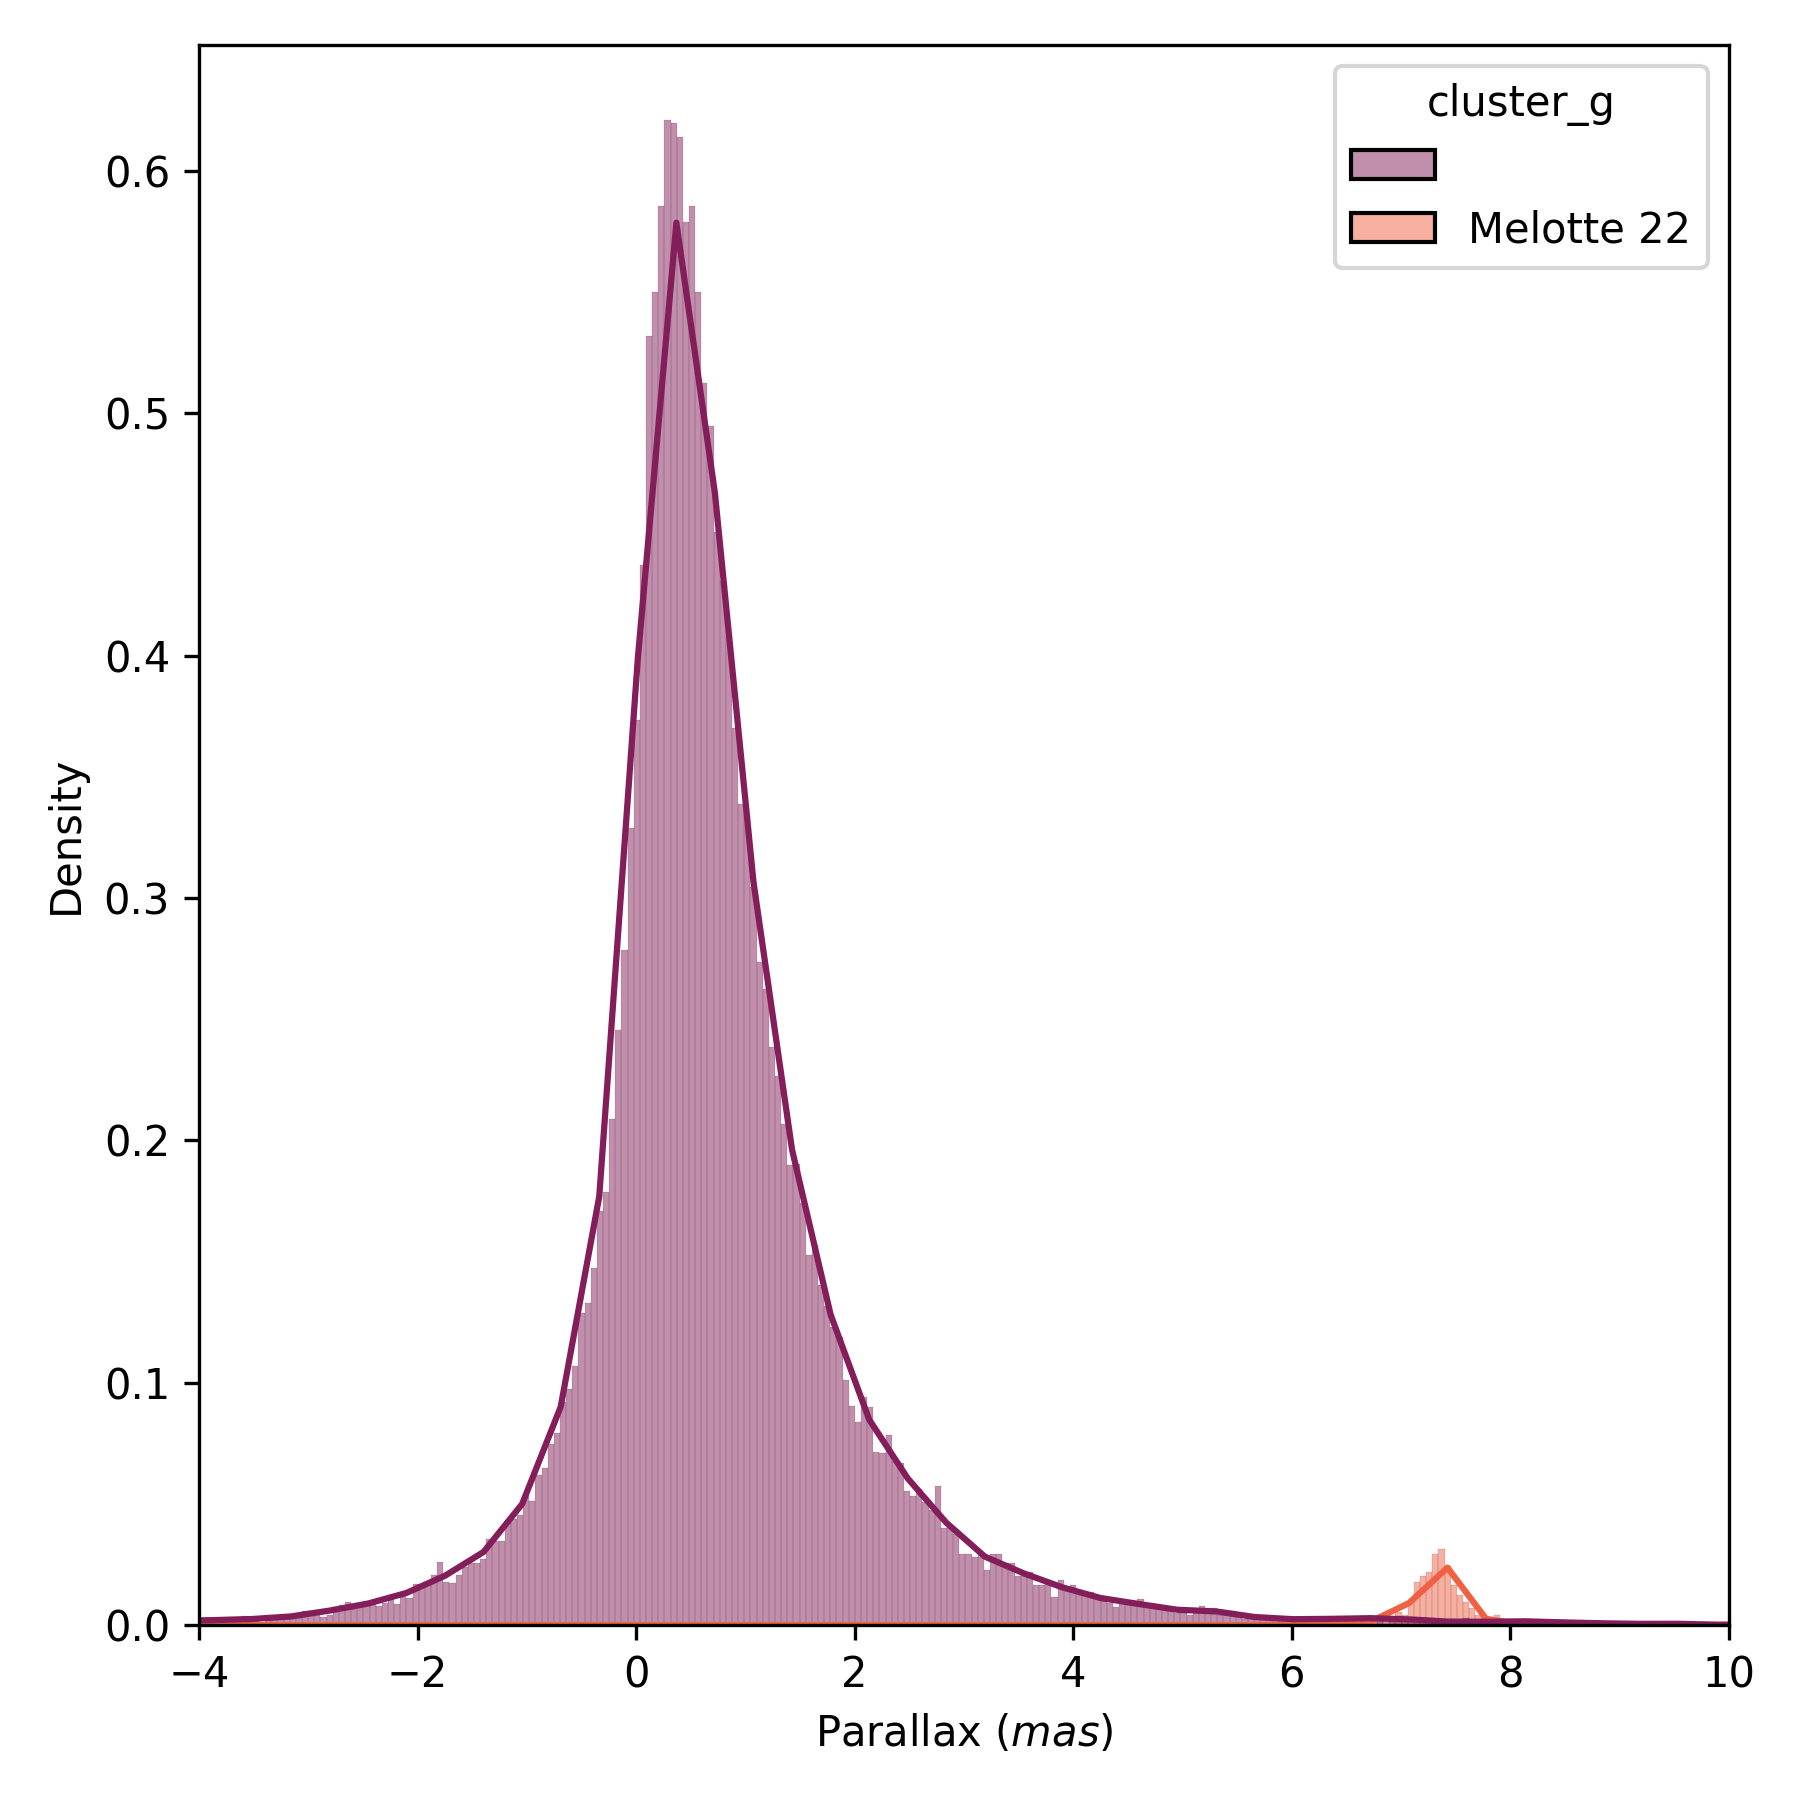
\includegraphics[width=\textwidth]{../figures/melotte_22/parallax_melotte_22.png}
      \caption{Parallax}
      \label{fig:pm_vec_melotte_22}
    \end{subfigure}
  \end{subfigure}
  \caption{Open Cluster Melotte 22 (Messier 45)}
\end{figure}

Figure~\ref{fig:pm_melotte_22} shows the proper motion distribution in right ascension and declination.
It is easy to see that a subgroup can be located at [20, -45].
Figure~\ref{fig:pm_vec_melotte_22} shows the parallax distribution and confirms an overdensity at
\(\approx 7.3 mas\) corresponding to Mellote 22 OC (See also Figure~\ref{fig:melotte_22_parallax_zoom}).

However, as shown in Figures~\ref{fig:pm_ngc_6494} and~\ref{fig:parallax_ngc_6494},
in general it is not as easy and becomes necessary to consider other parameters such as distances,
or even metallicity and age (derived from isochrone curves).
Sometimes even, photometric data may be required for the stars within the studied field.

\begin{figure}[htbp]
  \centering
  \begin{subfigure}{0.9\textwidth}
    \centering
    \begin{subfigure}[t]{0.45\textwidth}
      \centering
      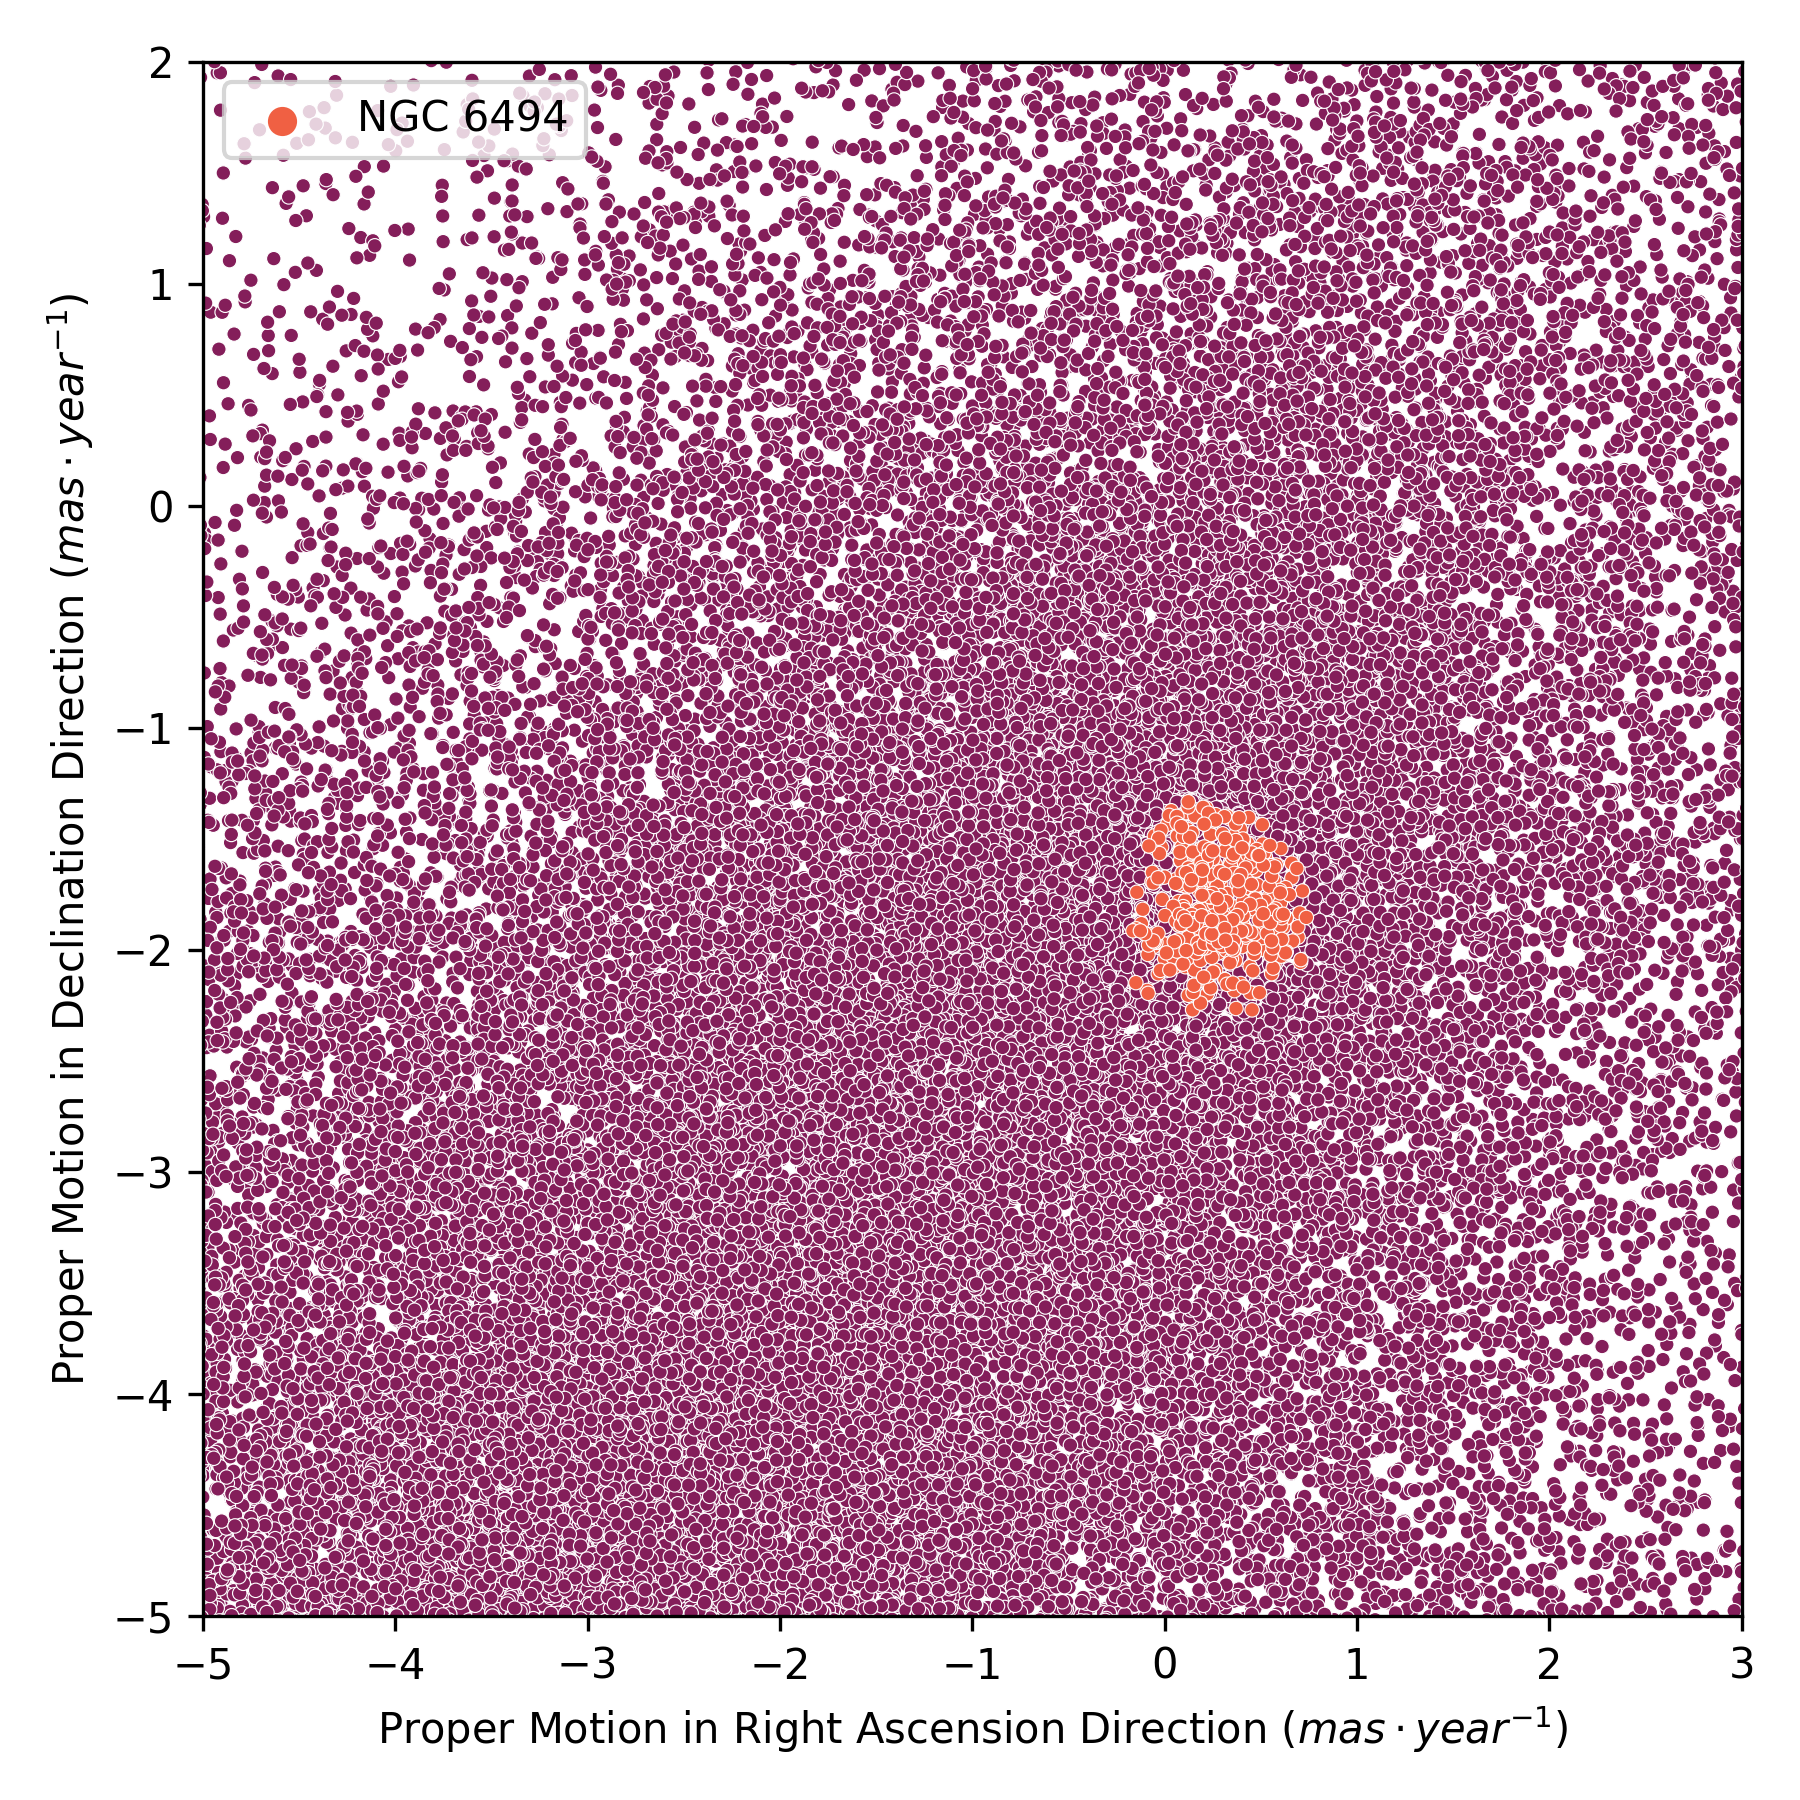
\includegraphics[width=\textwidth]{../figures/ngc_6494/pm_ngc_6494.png}
      \caption{Proper motions}
      \label{fig:pm_ngc_6494}
    \end{subfigure}
    \hfill
    \begin{subfigure}[t]{0.45\textwidth}
      \centering
      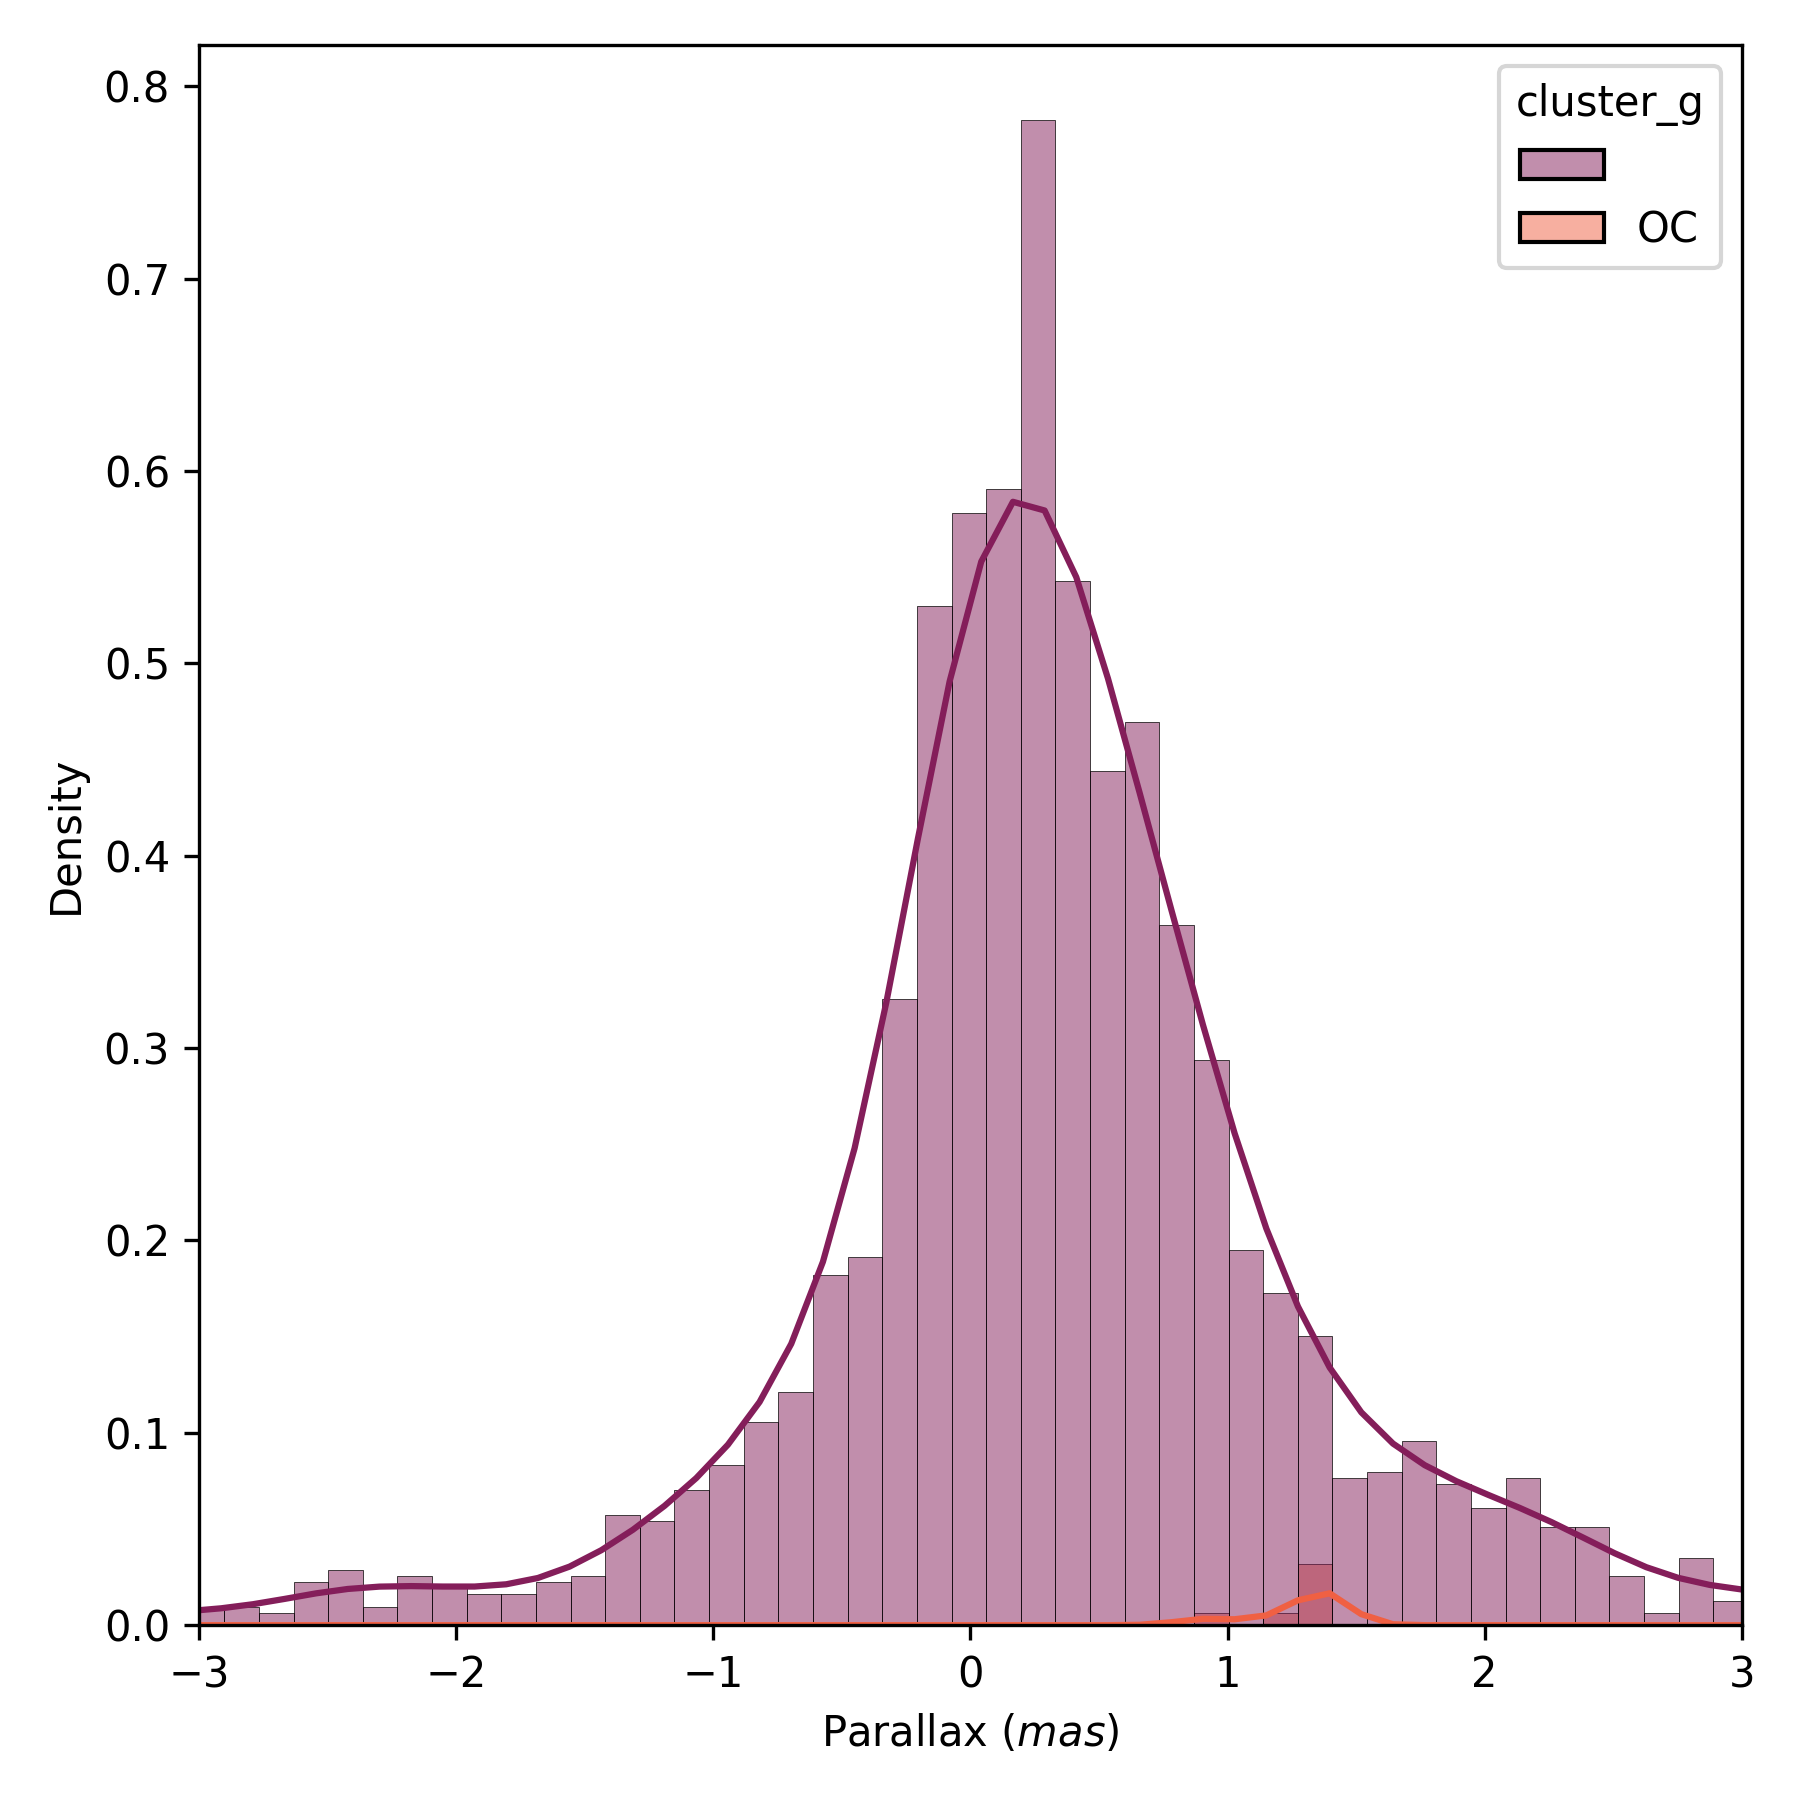
\includegraphics[width=\textwidth]{../figures/ngc_6494/parallax_ngc_6494.png}
      \caption{Parallax}
      \label{fig:parallax_ngc_6494}
    \end{subfigure}
  \end{subfigure}
  \caption{Open Cluster NGC 6494}
\end{figure}

At this point, it seems reasonable that the study of each individual group requires its own parametrization and technique
to identify it. With Gaia DR2, which contains high-quality astrometric and photometric data for a huge number of stars,
a new opportunity arises to simplify and optimize these processes. In this context, new approaches are being developed
to improve current detection methods and automate OC characterization.

\section{Gaia Mission}

In this work we make use of Gaia DR2 since DR3 has not been released in time for us to include it.
Gaia DR2 is a multidimensional dataset obtained by ESA's Gaia mission (located at L2, 1.5 million kilometers from Earth) and
operational since 2014. The catalogue has high precision and accuracy astrometric data for more than 1.7 billion stellar sources,
and magnitudes in three photometric filters (G, BP and RP) for more than 1,300 million sources.
80\% of Gaia DR2 sources are weaker than \(G_{mag} \approx 18\).
For magnitudes \(G \approx 21\) nominal uncertainties reach \(2 mas\) for parallaxes and \(5 mas \cdot years^{-1}\) in proper motions.
But for closer sources, (at the bright end, \(G < 14\)), the precision is of the order of \(0.02 mas\)
and \(0.05 mas \cdot year^{-1}\) respectively~\cite{cantat2018gaia}.
In general, open clusters, which are the main subject of this work, are at optimal data thresholds.

In this context, and taking advantage of the opportunity provided by Gaia DR2,
new approaches are being developed to improve current detection methods and automating OC characterization as much as possible.
This is the case of tools such as Clusterix 2.0~\cite{balaguer2020clusterix}, TOPCAT~\cite{taylor2005topcat}
and VOSA~\cite{bayo2008vosa}, (all of them developed by the Virtual Observatory).
These tools work together and offer good results,
although it is not possible to use them in an unsupervised process and they require different parameterizations for each study case.

\section{Current Methods}

TOPCAT by itself does not offer an independent discrimination mechanisms to researchers.
They have to try an initial selection, starting from the representation of proper motions,
by delimiting the area where the cluster most probably appears.
When this is not possible, it is necessary to have a previous knowledge about the cluster profile
and to parametrize some approximated values.
In both cases, the obtained selection must then be optimized step by step
until a result that meets the confidence levels is achieved.

Another tool is Clusterix 2.0, which is an interactive web-based tool~\cite{balaguer2020clusterix}.
It takes the proper motion diagram without making any prior assumption about the membership of the candidate star
and determines empirically the frequency functions.

Clusterix uses normal Gaussian kernel functions, defined as:

\begin{equation}
  K(a, b) = \frac{1}{2 \pi h^{2}} \exp{ \left[ - \frac{1}{2}\frac{\left( a - a_{i} \right)^{2} + \left( b - b_{j} \right)^{2}}{ h^{2}} \right]}
\end{equation}

\(\left( a, b \right)\) are referred to the proper motion configuration space,
while a point located in the center of the cell \(\left( i, j \right)\) provides the maximum
contribution for calculating the local density.
\(h\) is called the \emph{smoothing} parameter and it is measured in the same units as proper motion.

Various clustering algorithms have been studied in the past with the purpose of finding a valid non-parameterized method.
UPMASK~\cite{krone2014upmask} was developed to only use photometry and positions,
and then it was adapted to the Gaia data~\cite{cantat2018gaia} based only on proper motion and parallax.
A similar approach has been carried out using DBSCAN and machine learning algorithms to discover new clusters.

In this sense, Clusterix also claims to be a non-parameterized method,
but it critically depends on the initial selection for the field sizes to be analyzed.

\begin{figure}[htbp]
  \centering
  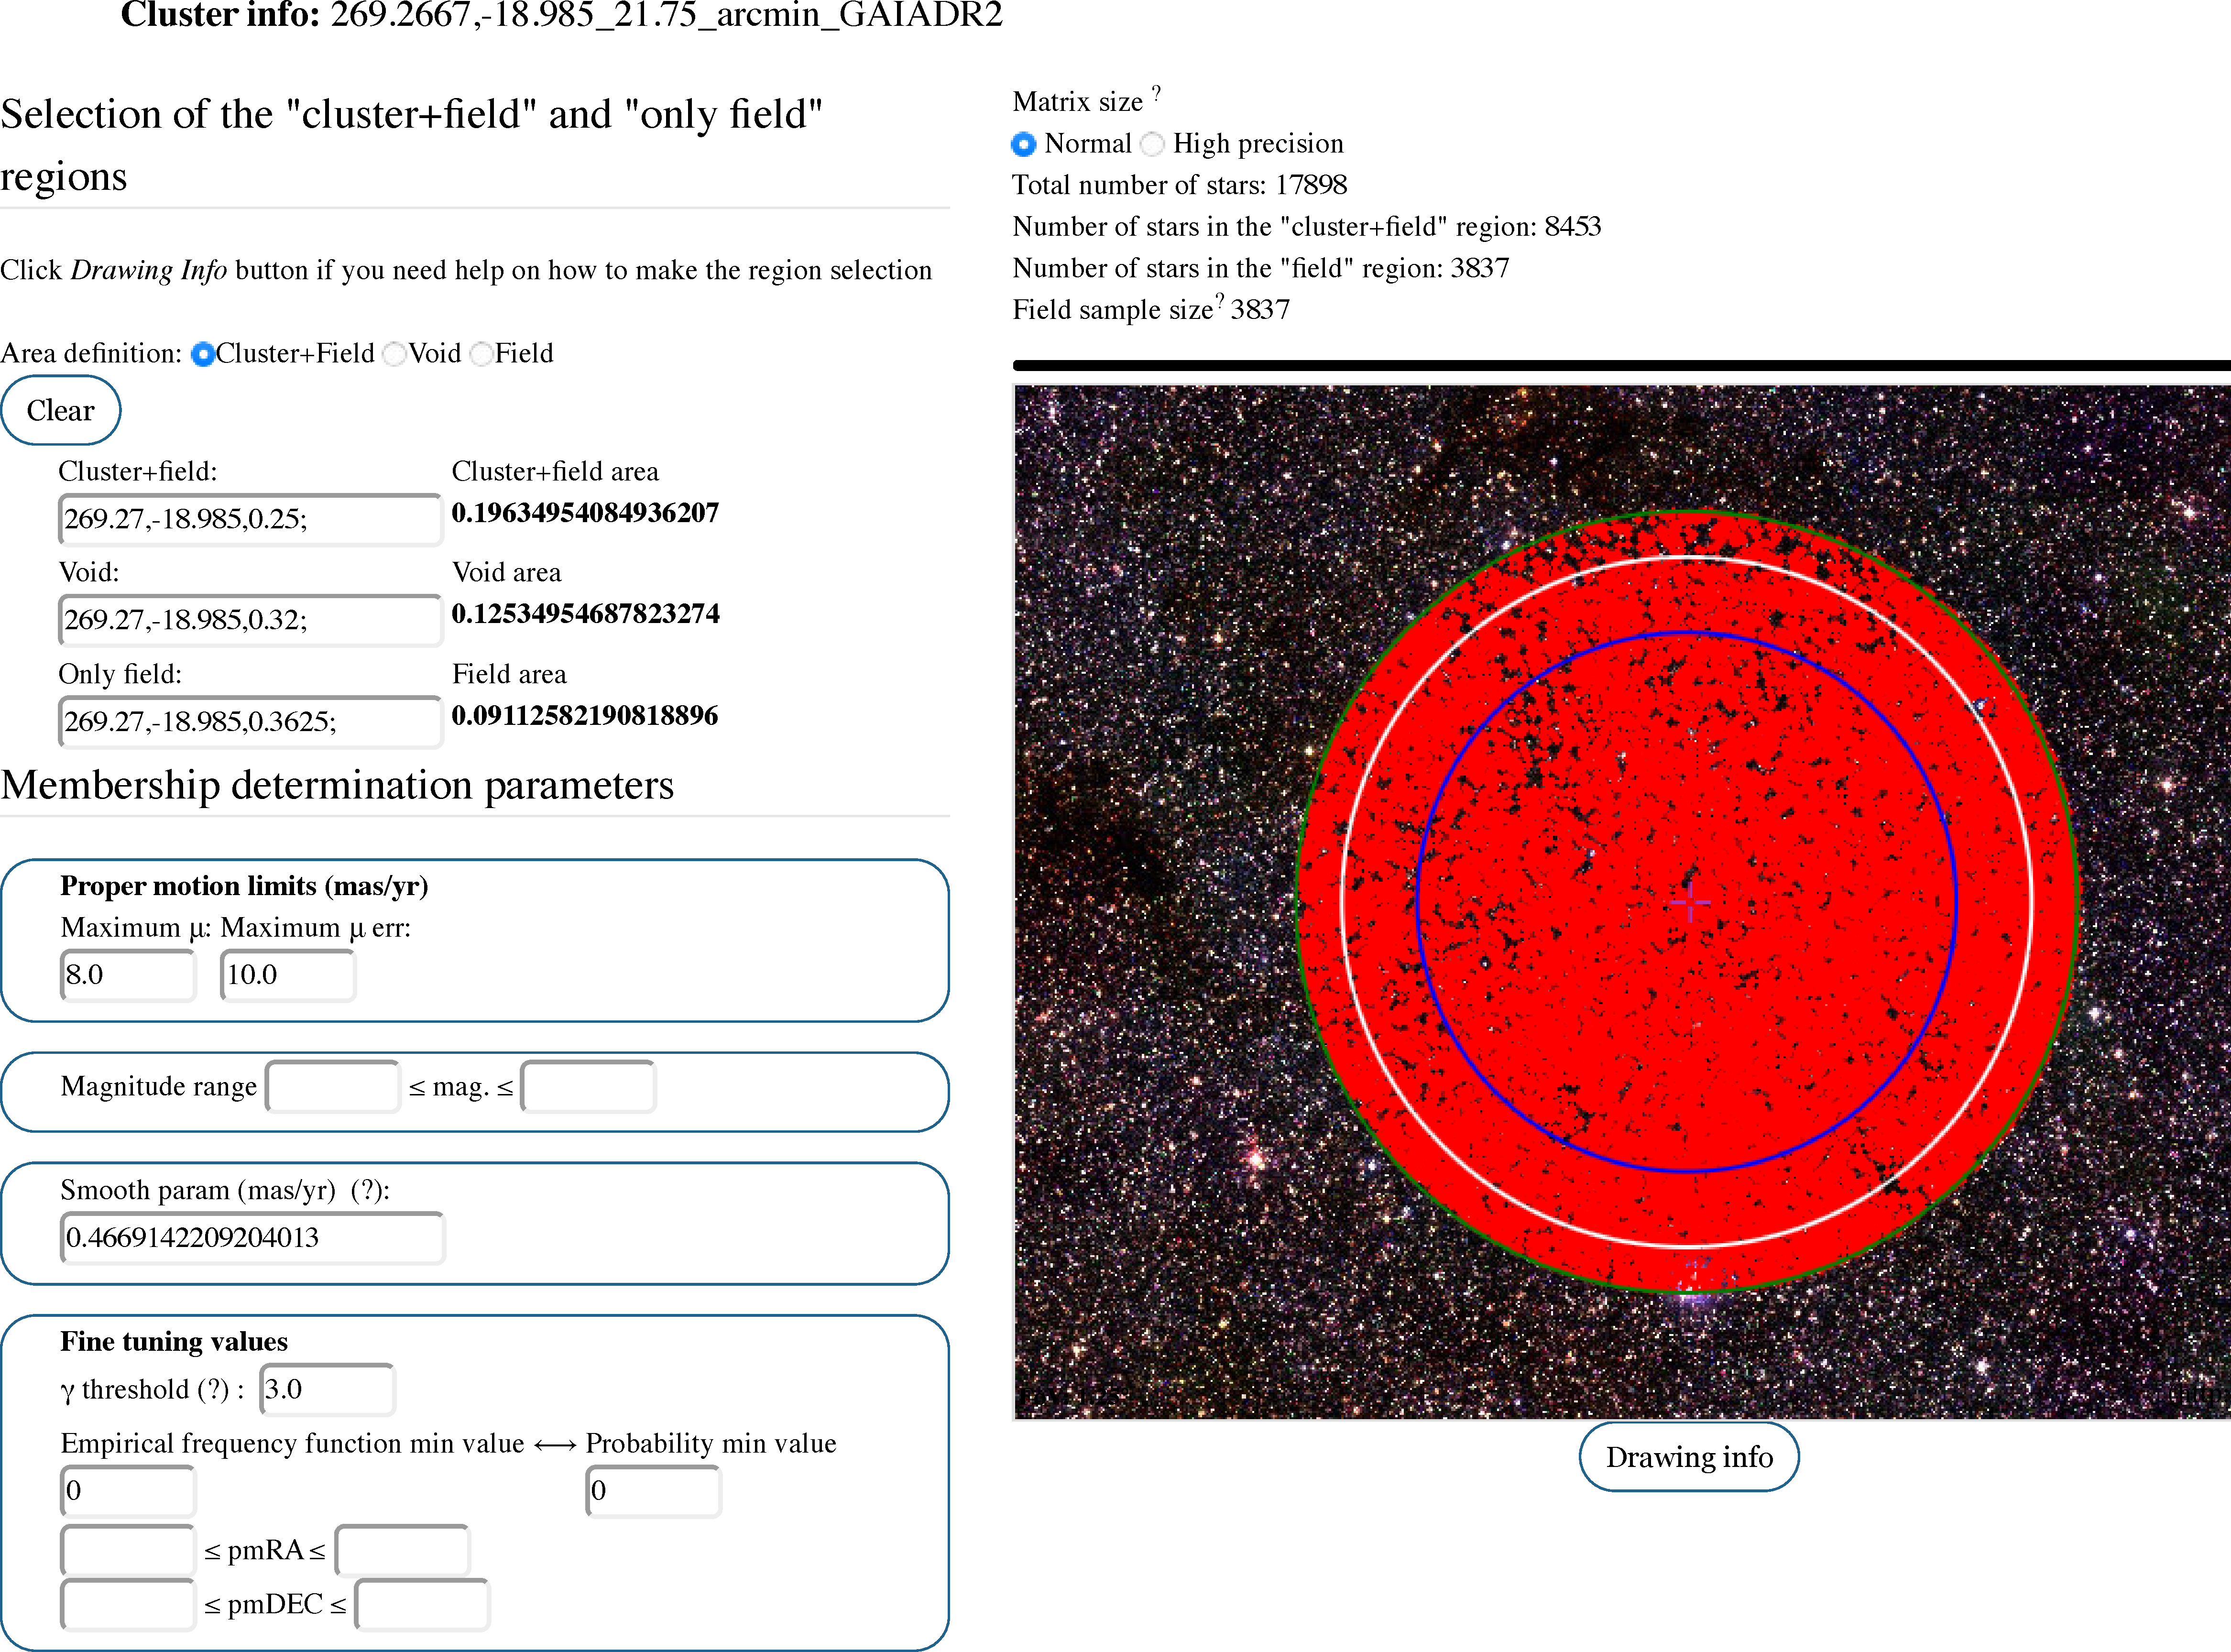
\includegraphics[width=0.9\textwidth]{../figures/clusterix/selection.pdf}
  \caption{Typical Clusterix 2.0 region selection panel.}
  \label{fig:clusterix_control_panel}
\end{figure}

Clusterix relies on several assumptions, among other:

\begin{displayquote}
The non-field population does not occupy the entire workspace, but is spatially concentrated,
which makes it possible to distinguish two regions in the workspace:
the only field region (label `f`), dominated by star fields,
and the cluster + field region (label `c+f`), which includes both star fields and not star
fields~\cite{balaguer2020clusterix}.
\end{displayquote}

This fact implies defining three areas or regions with different radius.
The first `c+f` corresponds to the one in which the cluster members are
presumed to be contained together with other star fields that are not part of the cluster.
The second region is the broadest and assumes that it only contains stars
in an extended visual field without components of the cluster.
The third region is the intermediate one and is out of analysis (void area),
since it would correspond to a possible transition zone between the other two.

The right choice of these radii, even having a previous estimation for the `c+f` region,
highly affects the execution of the algorithm and, in general, requires a considerable wide field `f`.
There is no rule of thumb that defines relative proportions of these areas.

Finally, when an acceptable result is obtained,
what Clusterix provides is a probability field associated to the set of stars under study.
The recovered dataset contains all fields from Gaia database
and an extra column with the probability value of each object to belong to the open cluster.
This new dataset can be exported to TOPCAT for further optimization and final processing.
Figure~\ref{fig:clusterix_probability} shows an example of the probability distribution
in the proper motion space for NGC 2682.

\begin{figure}[htbp]
  \centering
  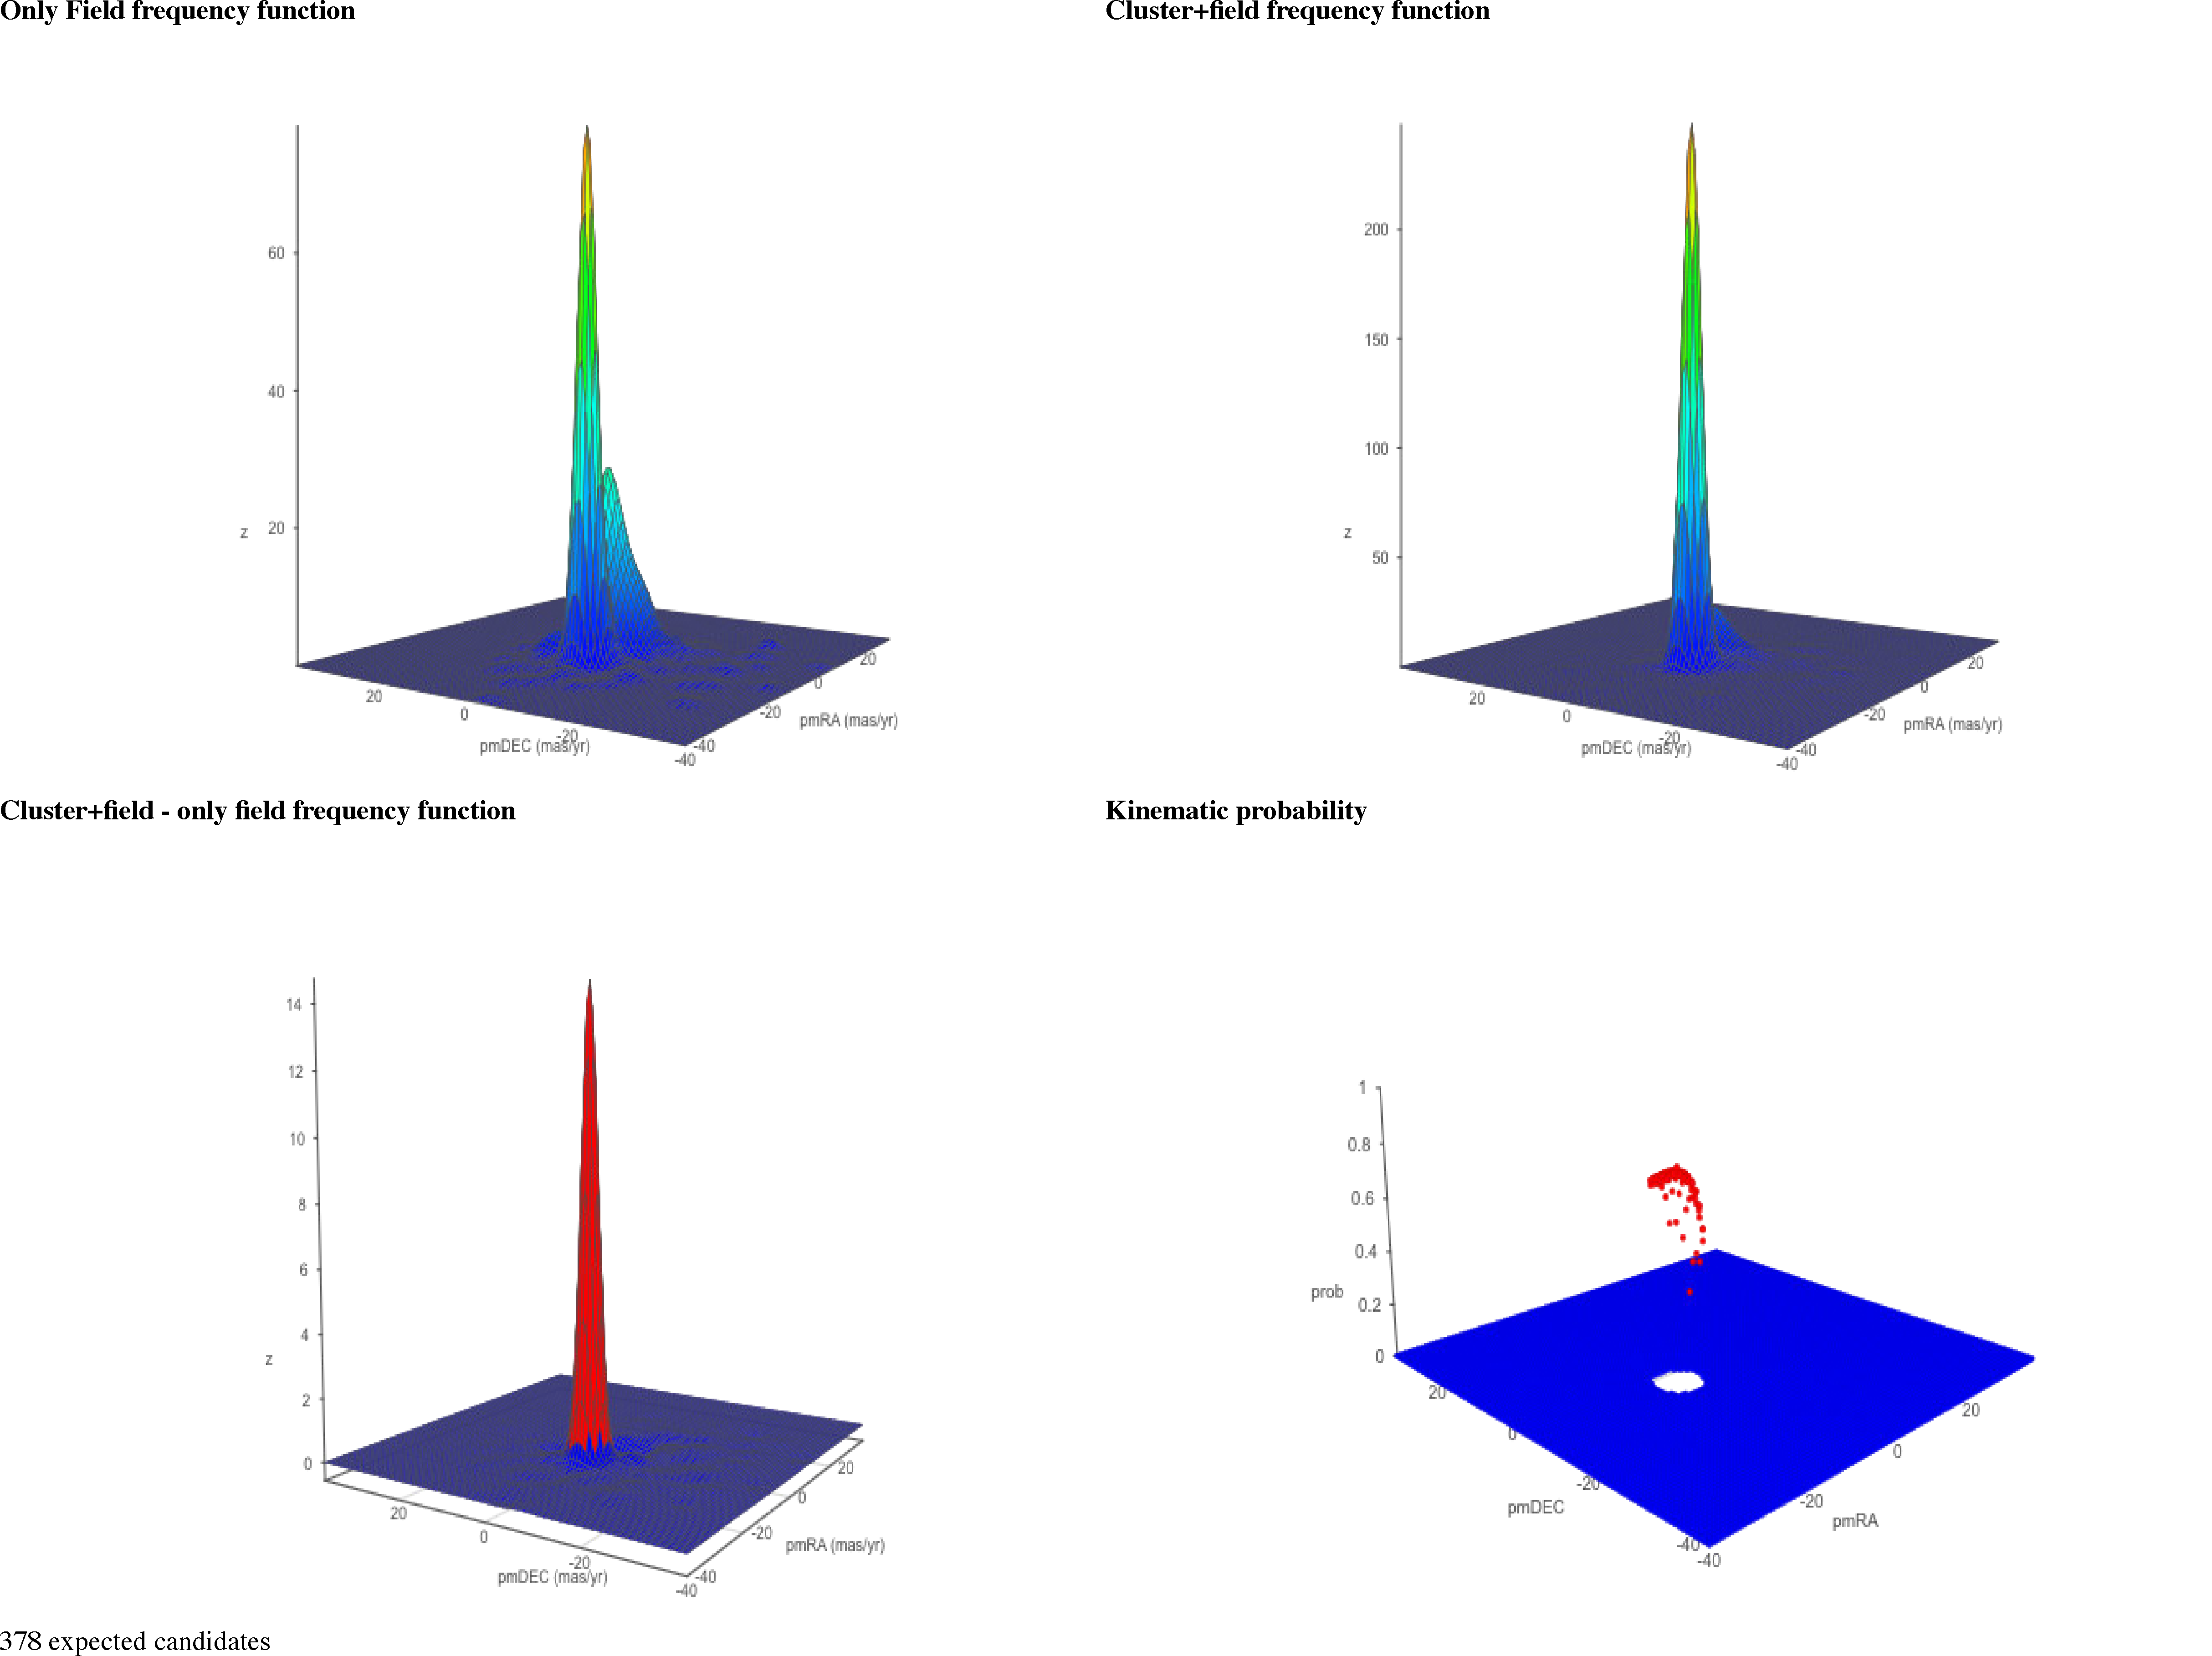
\includegraphics[width=0.9\textwidth]{../figures/clusterix/statistics.pdf}
  \caption{Probability distribution in the proper motion space provided by Clusterix for NGC 2682.}
  \label{fig:clusterix_probability}
\end{figure}

Finally, it is necessary to refer to the work developed on~\cite{castro2020hunting}.
It presents a method based on machine learning techniques to make a systematic search
for overdensities in the astrometric space of the galactic disk
and a later identification of OCs using photometric information, also from Gaia DR2.

The method includes two phases: the first one uses an unsupervised clustering algorithm, DBSCAN,
to search for overdensities \((l, b \pi, \mu_{\alpha} *, \mu_{\delta})\),
and then applies a deep learning Artificial Neural Network (ANN),
previously trained with magnitude diagrams,
to identify isochrone patterns within the detected overdensities and thus proceed to confirm them as OC.

It should be noted that for the execution of this method,
MareNostrum 42 (Barcelona Supercomputing Center) was used.
So the neural network could handle the image recognition process with isochrone patterns
and not applying theoretical models derived from values such as metallicity or masses, among other.

The result of this work is the recognition of 582 new open clusters
distributed along the galactic disk for a galactic declination \(b < 20^{\circ}\),
which has meant an increase of 45\% over previously ones.

Our aim in this work, linked to computational limitations compared to MareNostrum,
is not to perform a blind search for clusters, but to obtain a method, within the machine learning environment,
that allows the characterization of open clusters through unsupervised and non-parameterized procedures in a single step.
This method should not require further refinements with other tools.

The result of Clusterix + TOPCAT, applied to the same clusters,
will be used only for comparing and validating our results.

\section{Clustering Algorithms}

As we will explain later, what we need to accomplish our aim is an algorithm
that manages to make data groups based on the dynamic properties of the stars.

There are several clustering algorithms: \emph{K-Means}, \emph{Mean-Shift Clustering}, \emph{DBSCAN}~\cite{ester1996density} among other.
While each one behaves better according to the distribution of the objects to clusterize,
we have chosen K-Means by its simplicity and good results.

K-Means requires a single parameter, the number of clusters to build (\(N\)).
The algorithm looks for N center points which are vectors of the same dimension as the number of selected features.
K-Means starts by making an initial groups configuration and then,
it reassigns objects to other groups iteratively by minimizing the distance among points
inside the new group and maximizing the distance with the centers of the other groups.

The algorithm stops once a maximum number of iterations is reached,
or when changes between iterations is lower than a minimum.

This algorithm works well and gives good results at first approach.
However, we need to set a large number of clusters to find the open cluster we are looking for.
This fact complicates the identification of the OC and many times the found cluster contains to many outliers.
For that reason, we searched for a K-Means refinement based on an artificial neural network.

The \emph{Unsupervised Deep Embedding for Clustering Analysis} model
or \emph{DEC}~\cite{xie2016unsupervised} takes K-Means as its starting point,
but then, it trains an autoencoder to reduce the feature space
and pass this transformed data through a Clustering Layer which refines the previous selection.

The mechanism of this model is explained in Section~\ref{sec:deep_embedding_clustering}
and its implementation is available in \verb|cdalvaro.ml.dec| package.

\chapter{Method}
\label{chap:method}

In this chapter we address the different steps followed to perform the creation of
the unsupervised clustering model for open cluster characterization.

All code has been developed with the Python programming language~\cite{Python3}.
Other auxiliary tools like \emph{Docker}~\cite{merkel2014docker},
\emph{PostgreSQL}~\cite{postgresql}, \emph{Jupyter Notebooks}~\cite{Kluyver2016jupyter},
and frameworks such as \emph{Astropy}~\cite{astropy:2013}~\cite{astropy:2018},
\emph{Scikit-Learn}~\cite{scikit-learn}, \emph{Seaborn}~\cite{michael_waskom_2017_883859},
\emph{SQLAlchemy}~\cite{sqlalchemy} and \emph{Keras}~\cite{chollet2015keras} have been used too.

\begin{figure}[htbp]
  \centering
  \begin{subfigure}{0.5\textwidth}
    \centering
    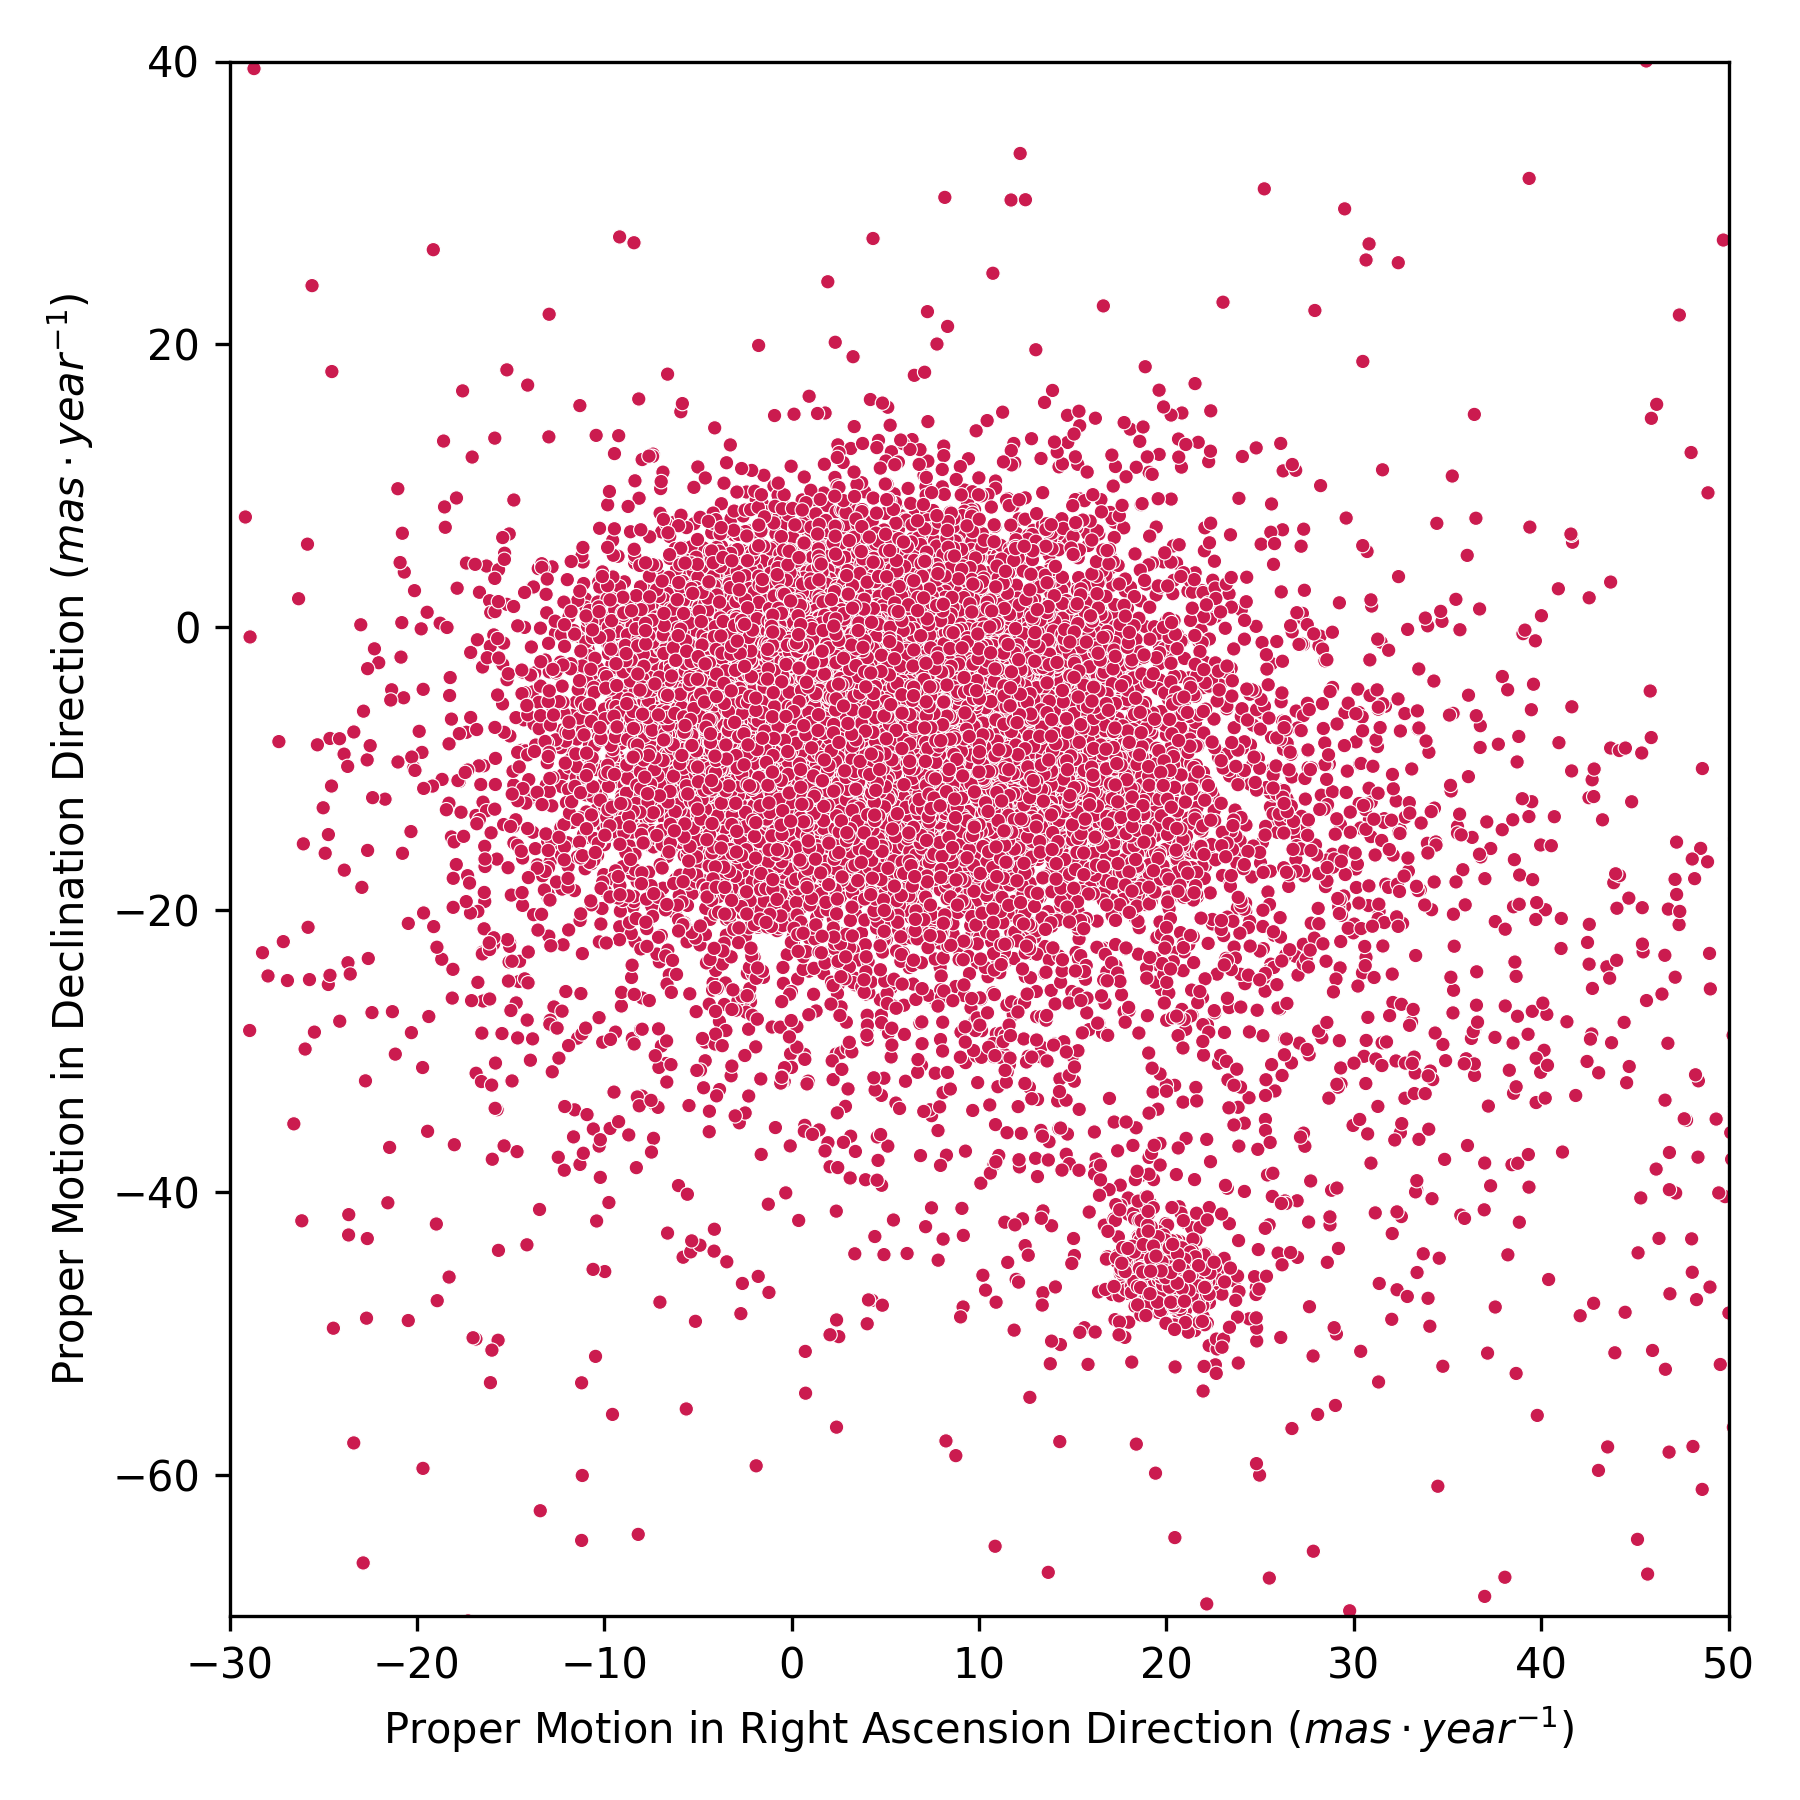
\includegraphics[width=\textwidth]{../figures/melotte_22/raw_pm_melotte_22.png}
  \end{subfigure}
  \caption{Melotte 22 proper motions}
  \label{fig:raw_pm_melotte_22}
\end{figure}

For the sake of simplicity, we are taking \emph{Melotte 22 (Messier 45)}~\cite{elsanhoury2019ppmxl} to illustrate the whole method.
This cluster is well studied and its stars are not too mixed with other stars that do not belong to the OC
although they are contained in the same observation field, so images look clear.

Figure~\ref{fig:raw_pm_melotte_22} shows \emph{proper motion in right ascension and declination}
for a sample of the downloaded dataset for Melotte 22.
At first sight, two main clusters can be distinguished, one of them centered nearly at (0, 0)
and the second one with center at (20, -45). This second cluster is the one we are looking for.

However, although the second cluster is almost isolated, there are stars that do not belong to the OC.
Thus, we need more information to properly characterize the open cluster.

\begin{figure}[htbp]
  \centering
  \begin{subfigure}{0.9\textwidth}
    \centering
    \begin{subfigure}[t]{0.45\textwidth}
      \centering
      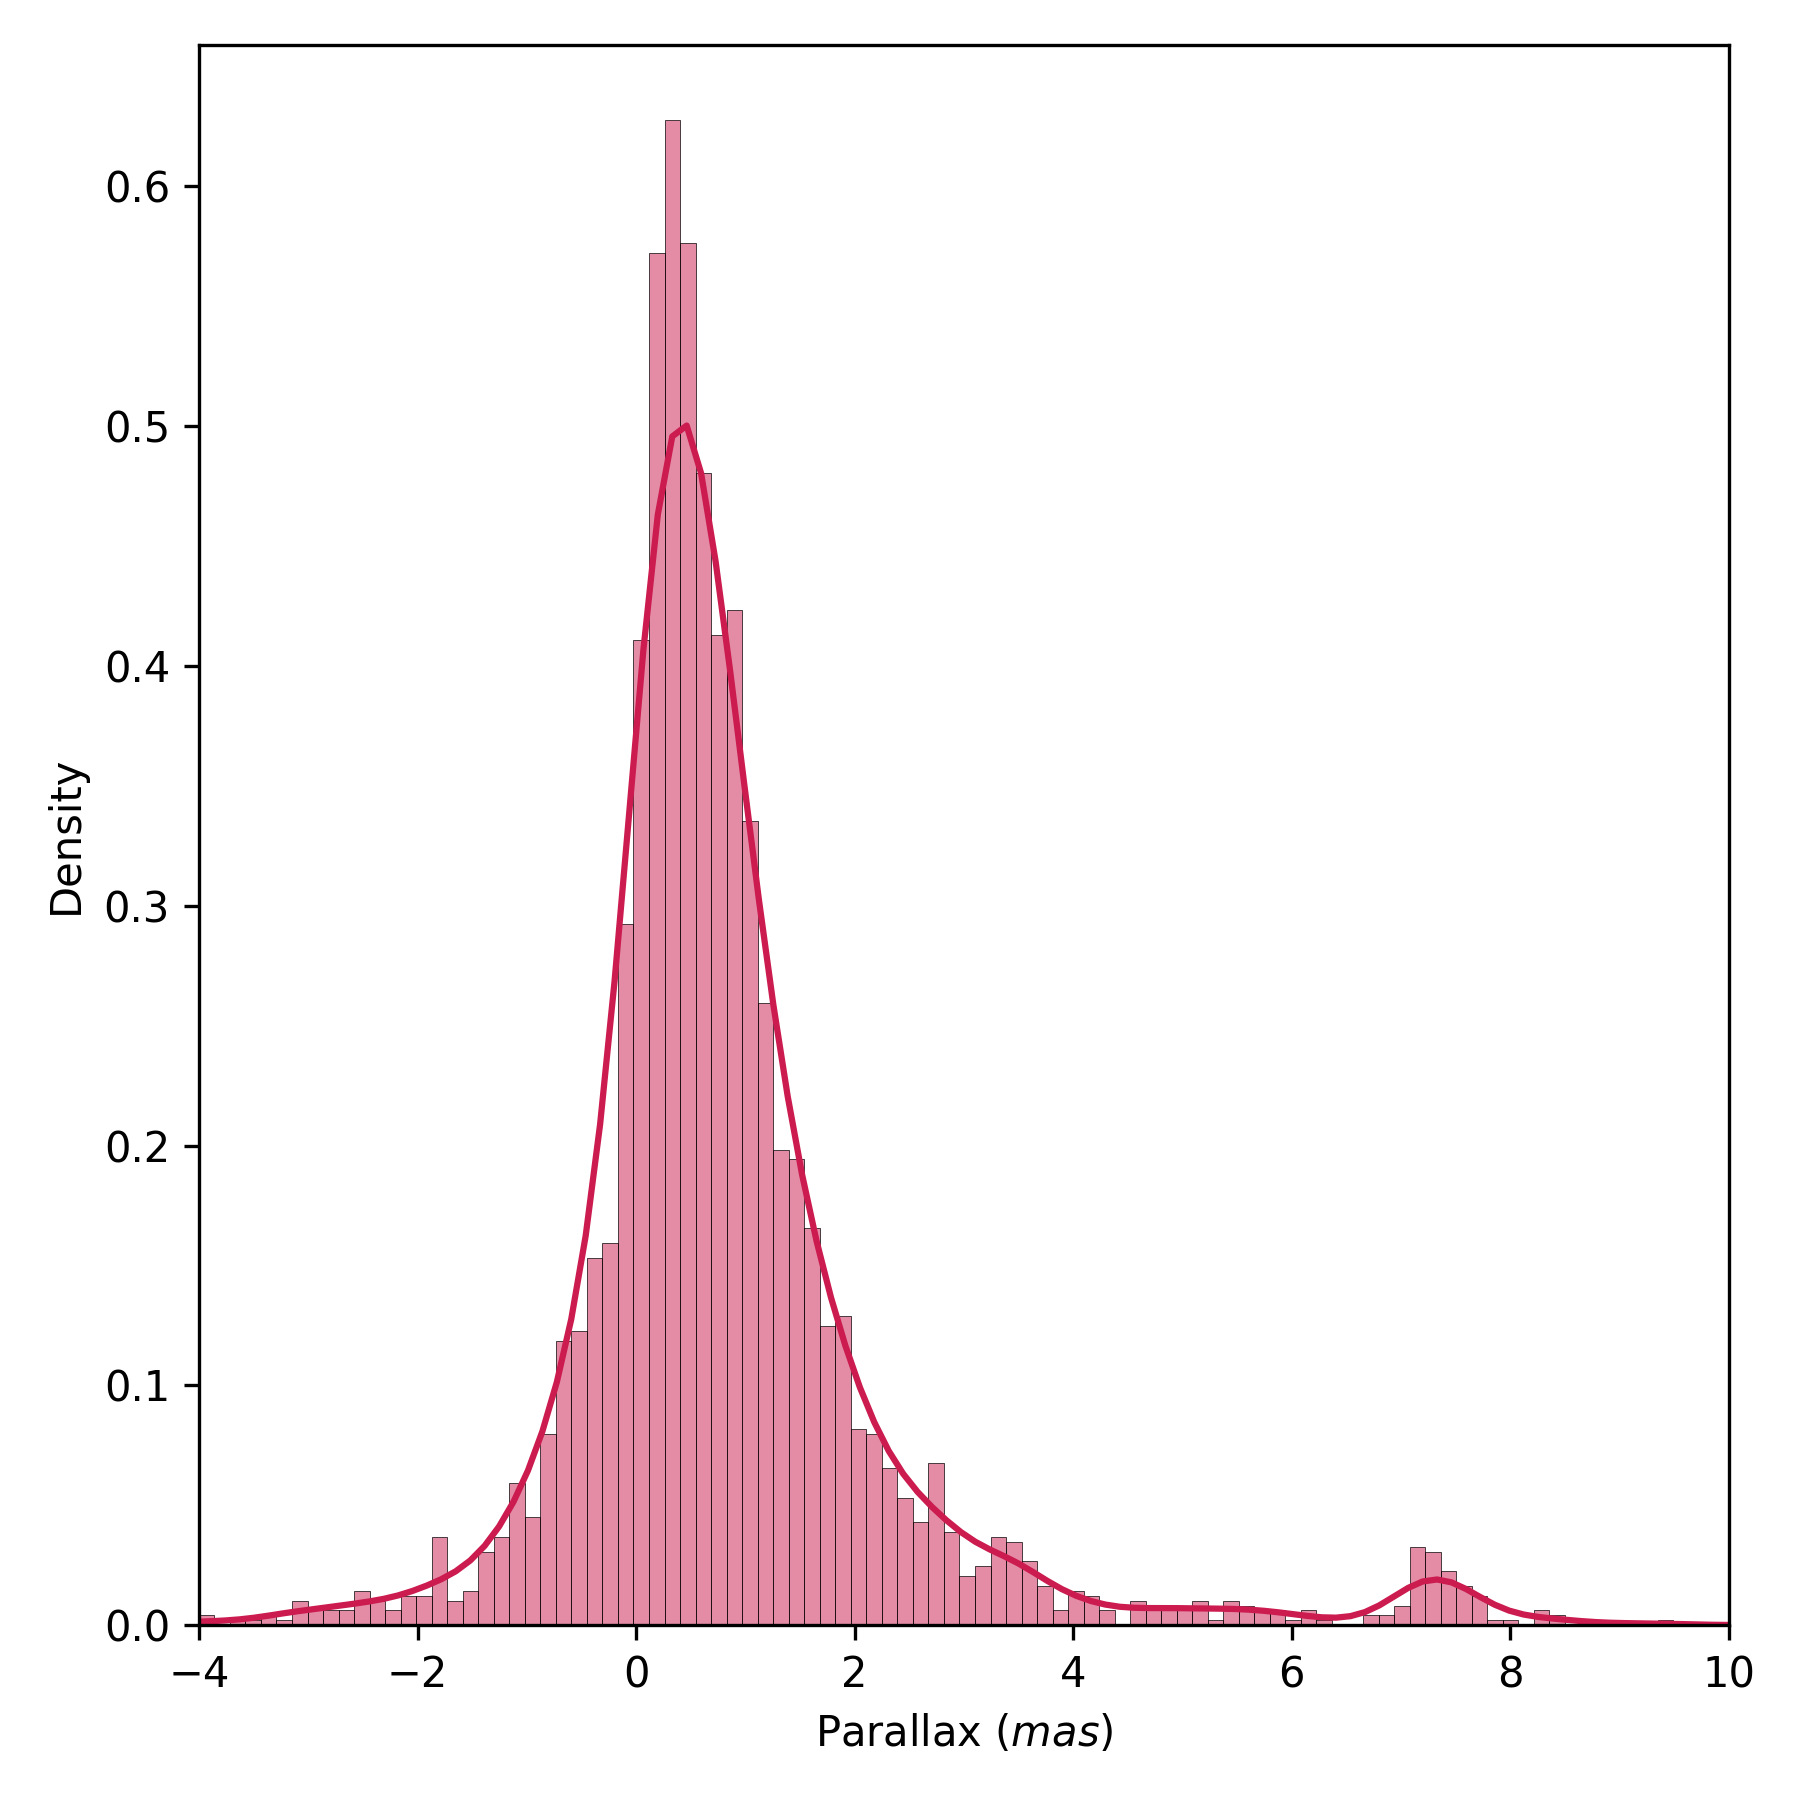
\includegraphics[width=\textwidth]{../figures/melotte_22/raw_parallax_melotte_22.png}
    \end{subfigure}
    \hfill
    \begin{subfigure}[t]{0.45\textwidth}
      \centering
      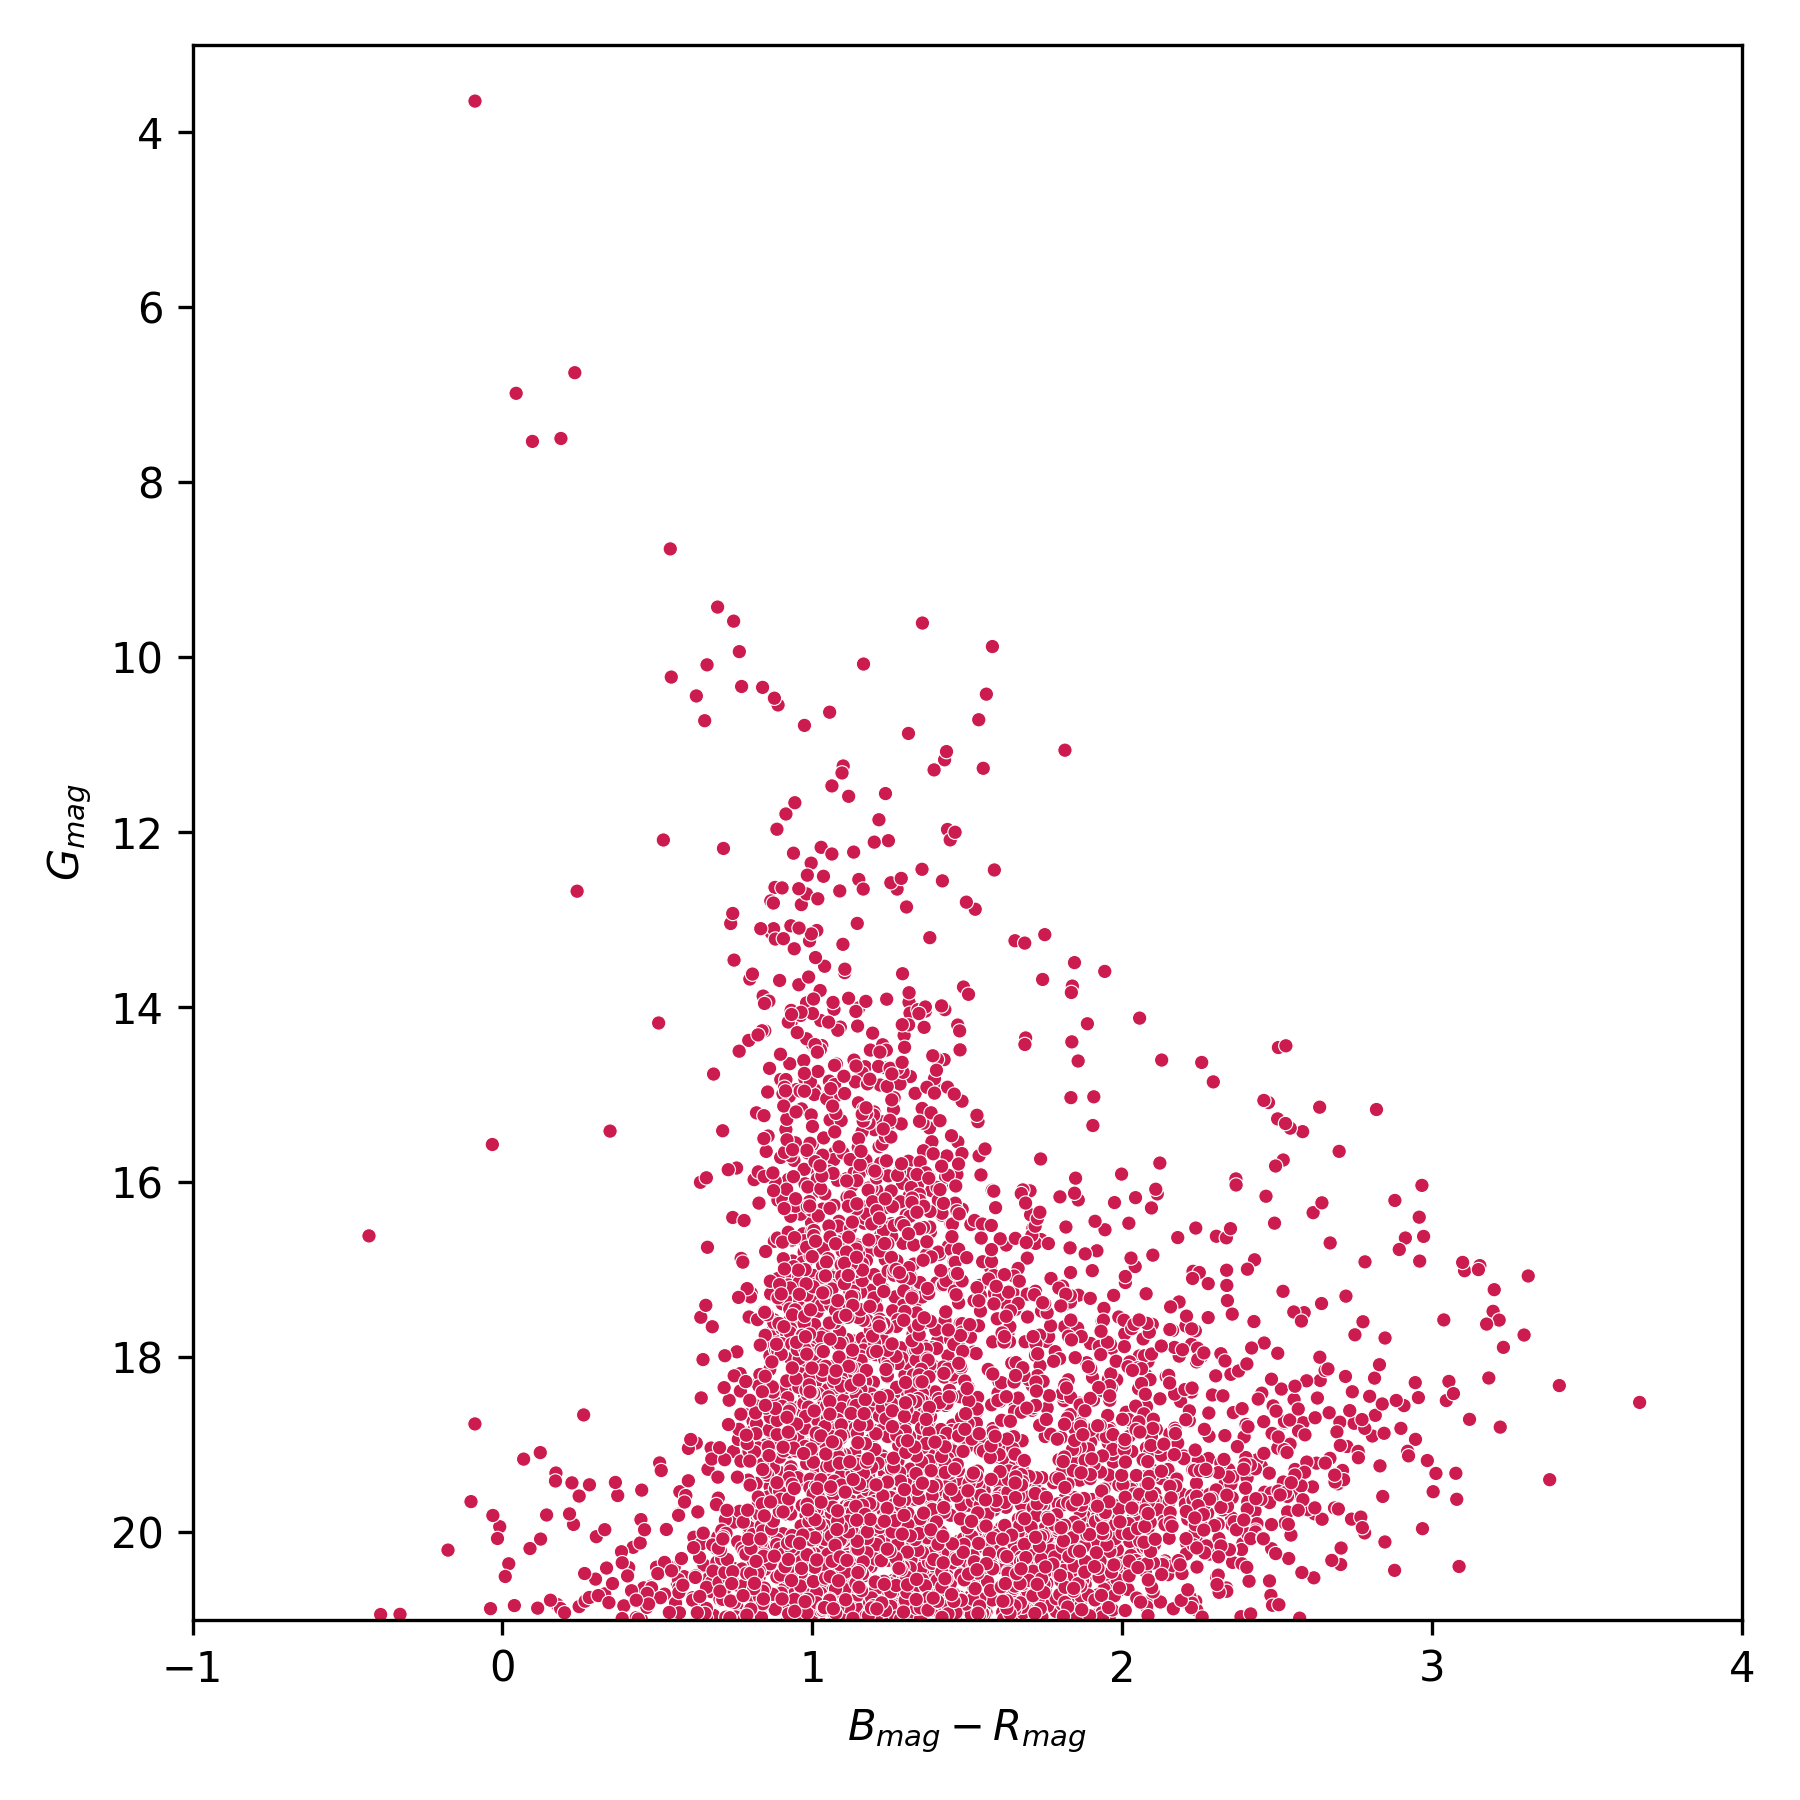
\includegraphics[width=\textwidth]{../figures/melotte_22/raw_hr_diagram_melotte_22.png}
    \end{subfigure}
  \end{subfigure}
  \caption{Melotte 22 parallax and H-R diagram}
  \label{fig:raw_parallax_hr_diagram_mellote_22}
\end{figure}

Figure~\ref{fig:raw_parallax_hr_diagram_mellote_22} shows the parallax histogram and the H-R diagram for this cluster, respectively.

The figure on the left shows a resonance at \(\approx 7.3mas\) belonging the OC.
While the figure on the right would help us to look for isochrone curves and so,
to determine the age of these stars.

\section{Data Mining}
\label{sec:data_mining}

Before being able to develop and test our clustering model,
the first step is to download the required data from the Gaia repository
and store it in a custom database for later access.

Due to the large amount of data available at Gaia, a complete download is not viable neither useful.
In order to reduce the size of the dataset to be downloaded,
the OpenClust catalogue~\cite{dias2002new} (Figure~\ref{fig:OpenClustComplete})
has been used to restrict the sky regions to be explored.

This download is not limited to the size registered in the catalogue.
Instead, a wider region (1.5 times the size of the cluster) is downloaded for each cluster to include stars outside the cluster.
The idea is that the unsupervised model must be able to clusterize those stars that belong to the OC
and to discard outsiders when characterizing the open cluster.

\begin{figure}[htbp]
  \centering
  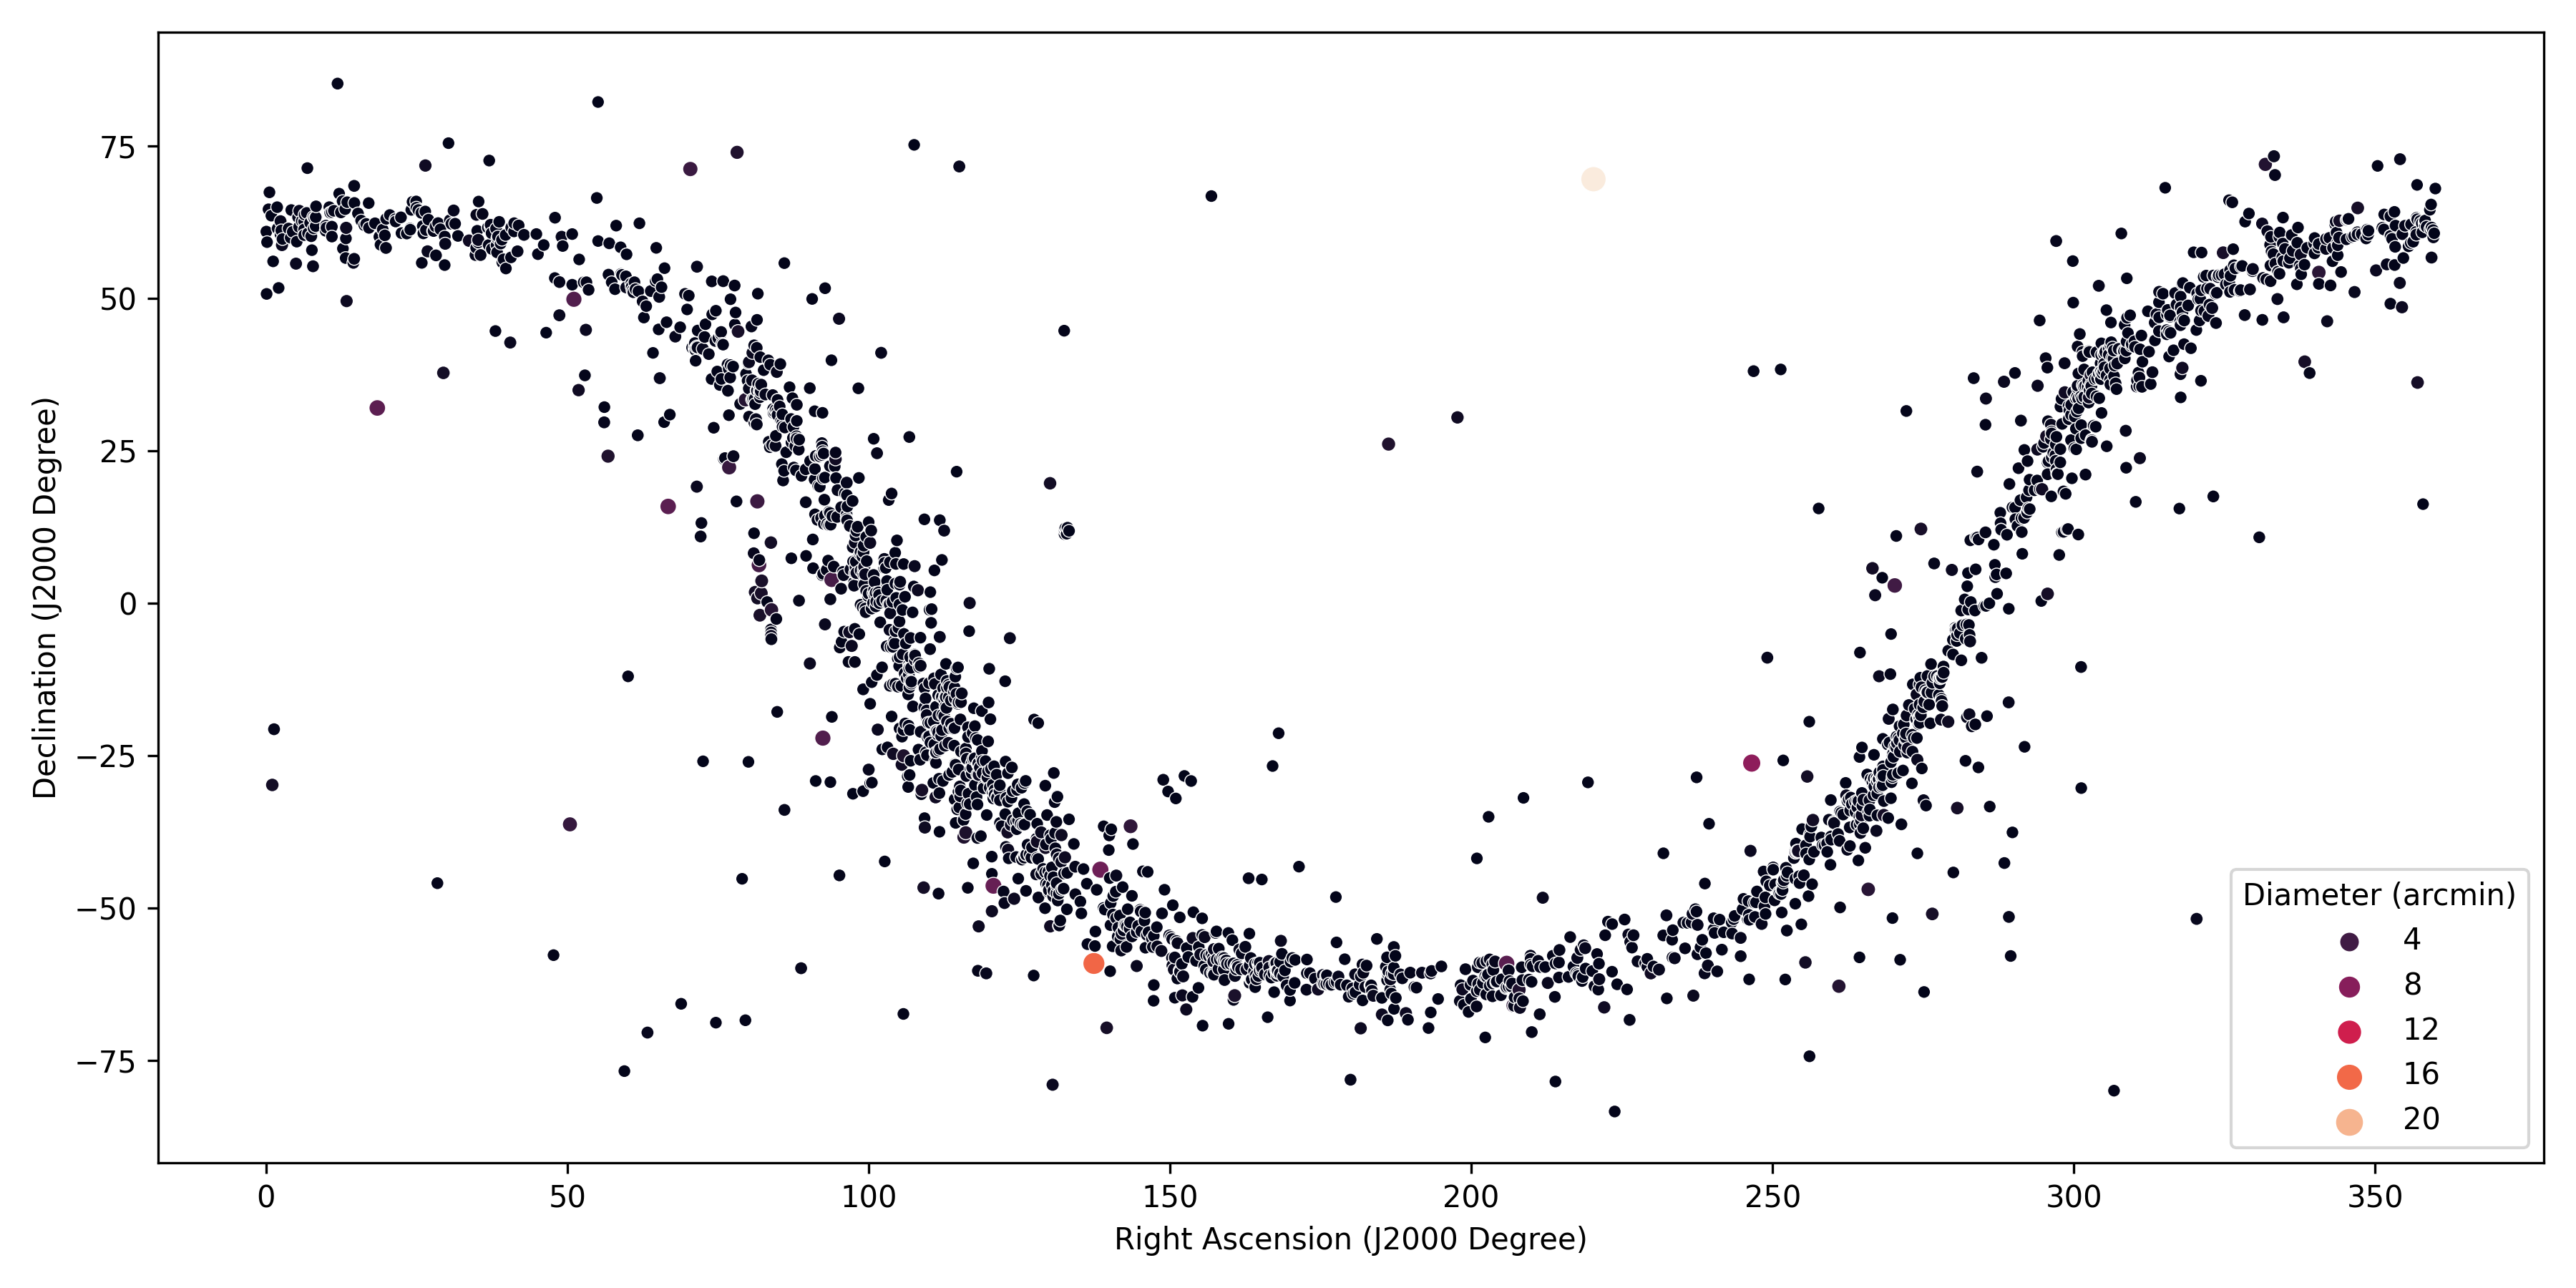
\includegraphics[width=0.9\textwidth]{../figures/openclust_catalogue.png}
  \caption{OpenClust Catalogue Distribution}
  \label{fig:OpenClustComplete}
\end{figure}

Taking these considerations into account, the downloaded dataset covers nearly 114 million stars (around 42GB of compressed data).
This dataset is significantly smaller than the whole Gaia DR2 dataset,
which contains information for approximately 1,600 million stars.
However, it is still too large.

Since not all the downloaded clusters are good enough,
we will apply a series of filters to discard clusters which do not have enough stars
or contain too many \emph{null} values.

Therefore, a cluster must fulfil the following filters in order to be accepted:

\begin{itemize}
  \item Cluster diameter above 25.0 arcmin
  \item Parallax absolute value greater than 0.0
  \item Number of stars\footnote{Every star must have all required features completely defined, i.e. without null values}
        in the selected region above 40,000 stars
\end{itemize}

As shown in Figure~\ref{fig:OpenClustSelection},
these constrains give us a smaller dataset but it is still a good representation of all clusters in the Milky Way
since they are equally distributed around the galaxy disk.

After having applied these filters, the number of cluster to analyze is 169 with nearly 75 million stars.

Since we have set no upper limit to the number of stars inside a cluster,
for the sake of simplicity and as a commitment to the project delivery dates
and the available computing power, smaller clusters will be preferred over the greatest ones.

As an extension of this work, the designed model could be applied to a region not covered by these constrains
for a later understanding of the results.

\begin{figure}[htbp]
  \centering
  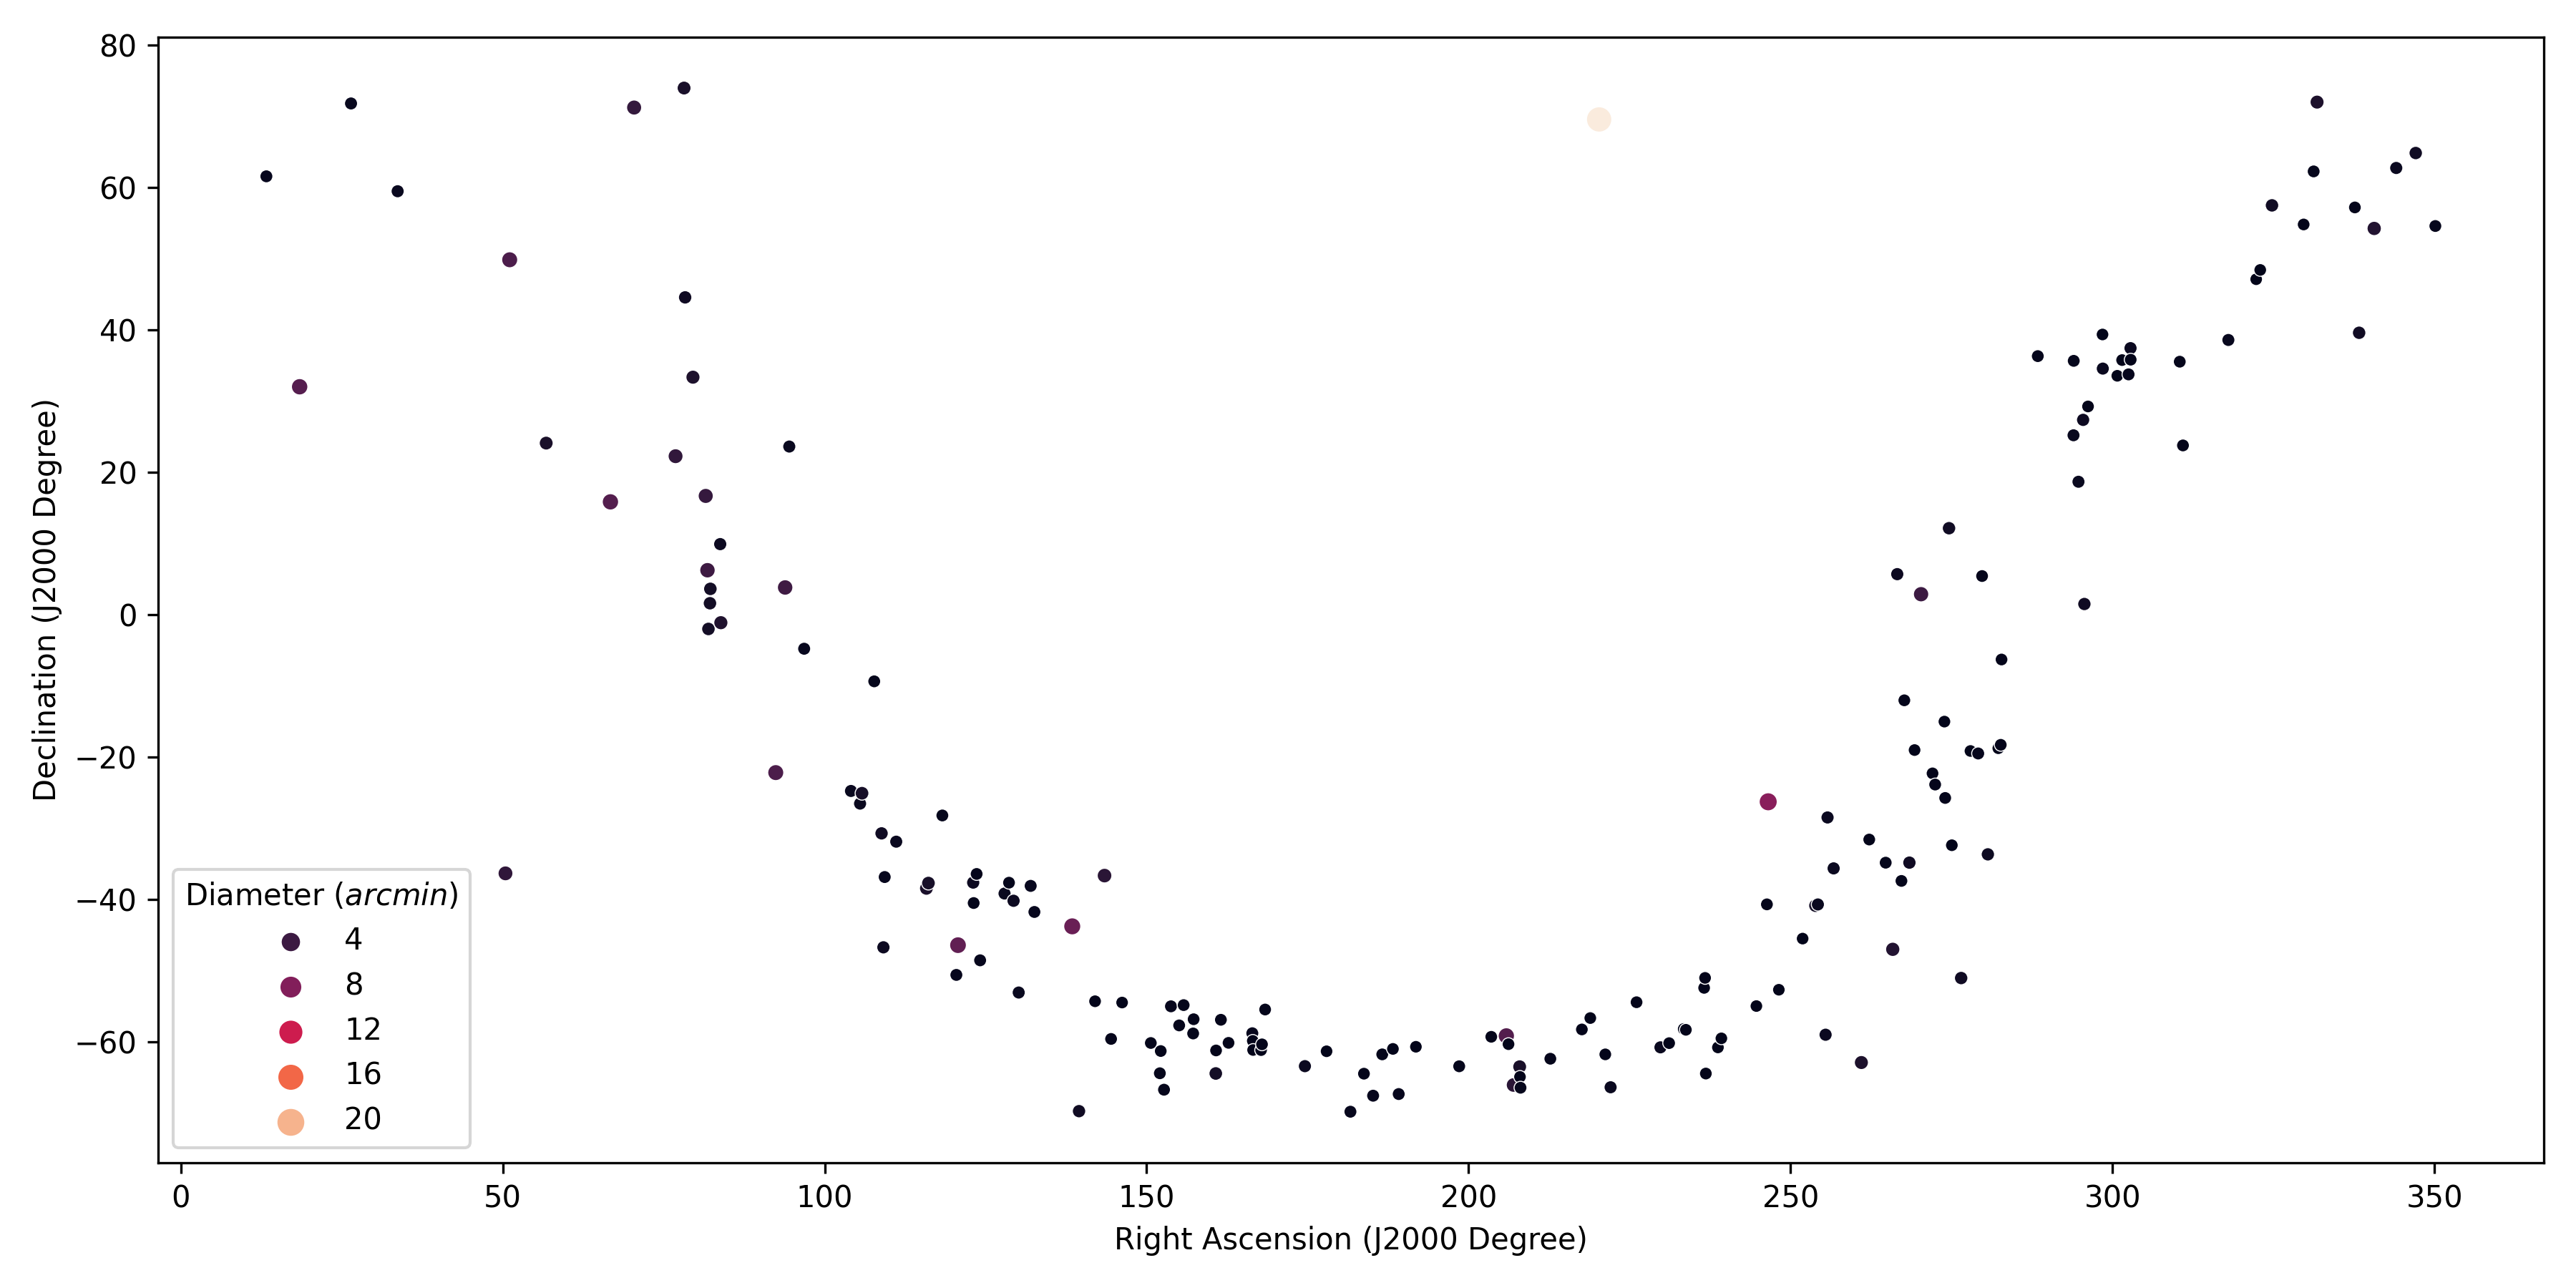
\includegraphics[width=0.9\textwidth]{../figures/cluster_selection_tier1.png}
  \caption{OpenClust Catalogue Selection Distribution}
  \label{fig:OpenClustSelection}
\end{figure}

\subsection{Download Process}

The download process has been performed with two Docker containers: a \emph{downloader} and the \emph{database}.

The first one is a container built from a \verb|python:3.8| image that contains the \verb|cdalvaro| package
and the \verb|downloader.py| script.
This script is prepared to load the OpenClust catalogue, connect to the Gaia DR2 database,
download all stars contained inside each cluster (with a radius factor to increase the area to be downloaded)
and save the downloaded data inside our custom database hosted in the second container.

\verb|downloader.Dockerfile| contains the build instructions for the downloader image.
We use \href{https://github.com/features/actions}{GitHub Actions} for automating the process
for building a new image version with every new push made to the \verb|main| branch.

This image can be pulled from the
\href{https://github.blog/2020-09-01-introducing-github-container-registry/}{GitHub Container Registry}:

\begin{minted}{sh}
  docker pull ghcr.io/cdalvaro/gaia-downloader:latest
\end{minted}

The second container is just a \verb|postgres:12.4| image which loads an initial script when
the database is not yet initialized for creating the database schema.
This container is used later as the main database for data analysis.

\begin{figure}[htbp]
  \centering
  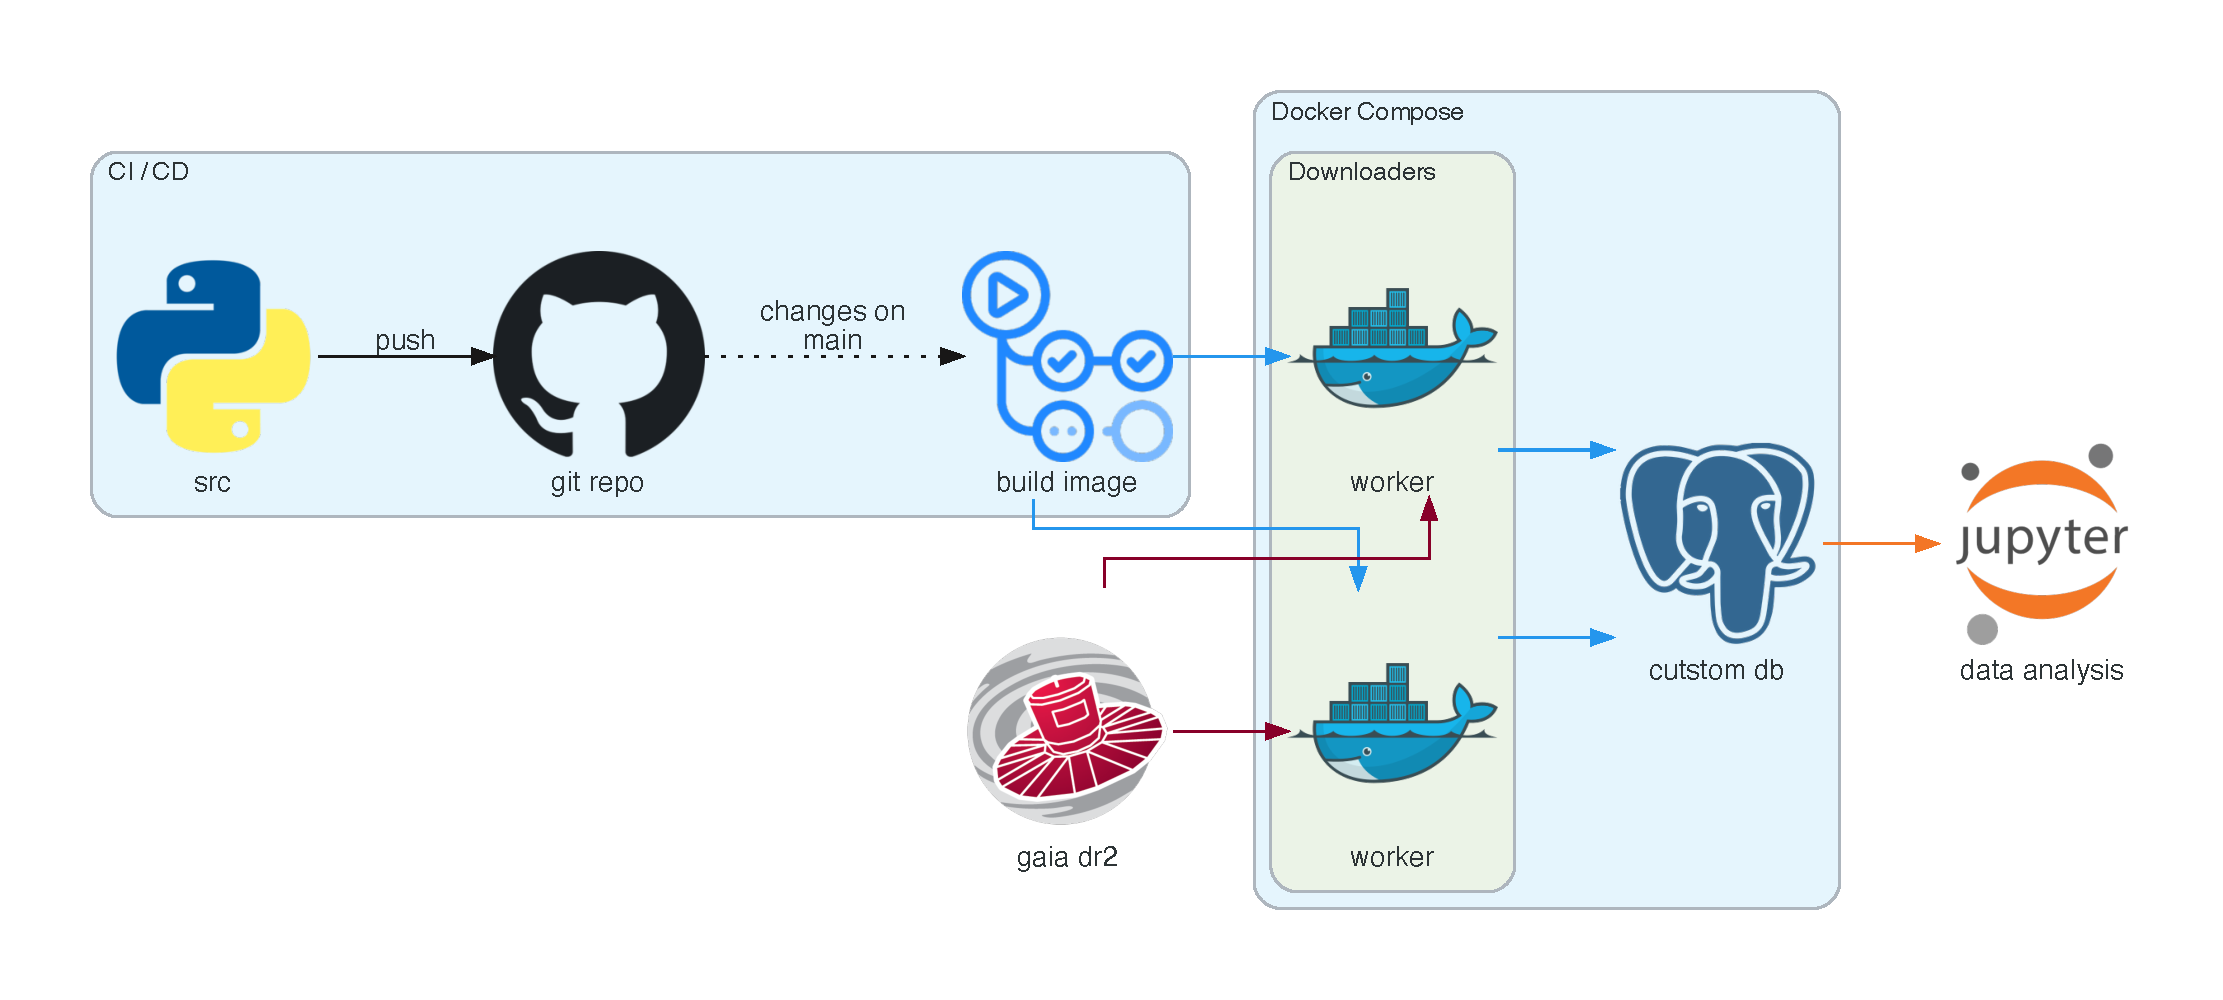
\includegraphics[width=0.9\textwidth]{../figures/services_diagram.pdf}
  \caption{Data retrieval and analysis}
  \label{fig:services_diagram}
\end{figure}

These containers are orchestrated with a \verb|docker-compose.yml| file which automatically launches one instance of each container.
Figure~\ref{fig:services_diagram} shows a diagram describing the services architecture for this work.

The database has two main tables in \verb|public| schema:

\begin{itemize}
  \item \verb|public.regions| for storing cluster properties such as \emph{location}, \emph{diameter} and other properties
  \item \verb|public.gaiadr2_source| which contains data for all downloaded stars from Gaia
\end{itemize}

\begin{figure}[htbp]
  \centering
  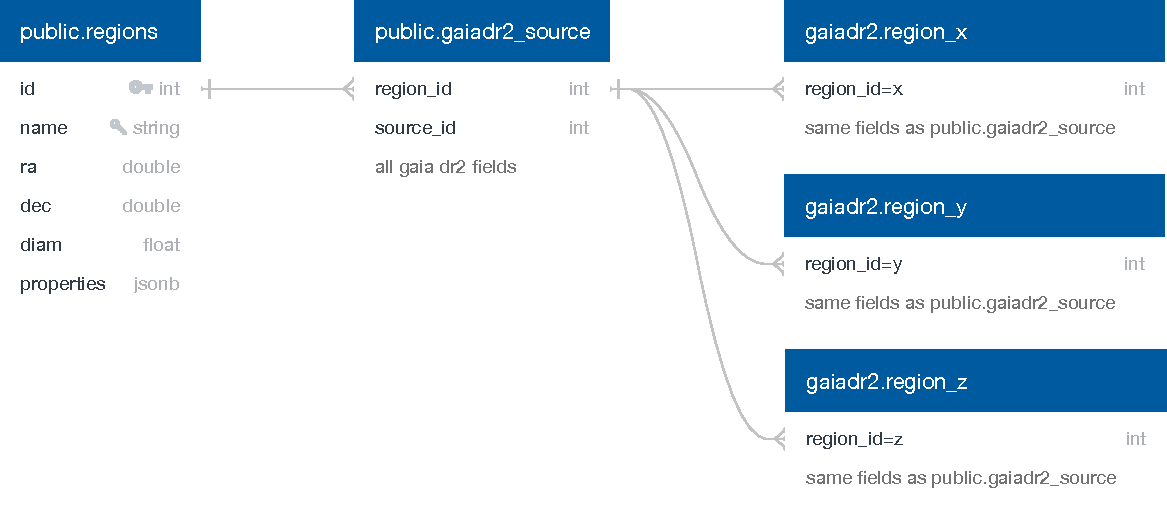
\includegraphics[width=0.9\textwidth]{../figures/customdb_diagram.pdf}
  \caption{Custom DB diagram}
  \label{fig:customdb_diagram}
\end{figure}

The second table is partitioned by region,
storing all stars related to one region inside an independent table for optimized access performance.
Partition tables are located inside \verb|gaiadr2| schema. See Figure~\ref{fig:customdb_diagram}.

Although \verb|public.gaiadr2_source| is partitioned, there is no need for us to directly access to one of those tables.
We only need to know the \verb|id| for the desired region and query for its stars to the main table as follows:

\pagebreak

\begin{minted}{sql}
  -- Get region id
  SELECT id FROM public.regions WHERE name = 'Melotte 22';
  -- output: id -> 302

  -- Get stars for the given id
  -- NOTE: PostgreSQL cannot optimize this query when region_id is
  --       provided as a subquery. This is why we get first the region id.
  SELECT * FROM public.gaiadr2_source WHERE region_id = 302;
\end{minted}

PostgreSQL knows that all stars we want are located inside \verb|gaiadr2.region_302| so it does not need to query any other table.
This allows us to download data for as many regions as we want without loosing performance when accessing for that data.

\verb|gaiadr2_source| and its partitions contain all fields available at the Gaia DR2 database.
A complete list of these fields and their description can be found at the following link:
\sloppy\url{https://gea.esac.esa.int/archive/documentation/GDR2/Gaia_archive/chap_datamodel/sec_dm_main_tables/ssec_dm_gaia_source.html}

Table~\ref{tab:important_fields} shows a brief description of the fields used in this work.

\begin{table}[h!]
  \begin{center}
    \begin{tabular}{r|c|l}
      \textbf{Name} & \textbf{Units} & \textbf{Description} \\
      \hline
      \verb|ra| & Angle [deg] & Right ascension \\
      \verb|dec| & Angle [deg] & Declination \\
      \verb|parallax| & Angle [mas] & Parallax \\
      \verb|pmra| & Angular Velocity [mas/year] & Proper motion in right ascension \\
      \verb|pmdec| & Angular Velocity [mas/year] & Proper motion in declination \\
      \verb|phot_g_mean_mag| & Magnitude [mag] & G-band mean magnitude \\
      \verb|bp_rp| & Magnitude [mag] & BP - RP colour \\
    \end{tabular}
    \caption{Properties and descriptions of the fields used in this work.}
    \label{tab:important_fields}
  \end{center}
\end{table}

The downloader takes data from the Gaia DR2 database and saves the selection into our custom database without modifying any value,
so data preserves all its properties and units.

Python methods for retrieving information from the database are available through an instance of \verb|cdalvaro.DB|.
This class contains methods for retrieving star's information for a given region as a Pandas \verb|DataFrame|, ready for data analysis.

The developed code for this work can be found inside the \verb|src| directory at GitHub:
\href{https://github.com/cdalvaro/machine-learning-master-thesis}{cdalvaro/machine-learning-master-thesis} repository.
(For the printed version of this work, you can scan the QR code on cover for accessing it.)

\section{Feature Selection}
\label{sec:feature_selection}

As mentioned before, we want our model to characterize open clusters by looking at their dynamic properties.
Also, we want to maintain as simple as possible our clustering model in order to save computing resources.

Proper motion in right ascension and declination seems like a natural choice since, as we know,
stars belonging to the same OC share a common motion vector.

Parallax is another important feature. It lets us know how far stars are from the Earth.
In addition, since all stars within an open cluster were born from the same dust cloud,
they must all have similar parallax.

However, we are not going to use these raw features. Instead, we are taking a combination of them.

First, we correct proper motion in right ascension and declination by dividing them by the parallax.
That way, we normalize these quantities and help our clustering models to improve their performance.

The modulus of the proper motion is another computed property that we are considering.
We use it to relate both features and therefore, to force our model to keep them tight.

\begin{figure}[htbp]
  \centering
  \begin{subfigure}{\textwidth}
    \centering
    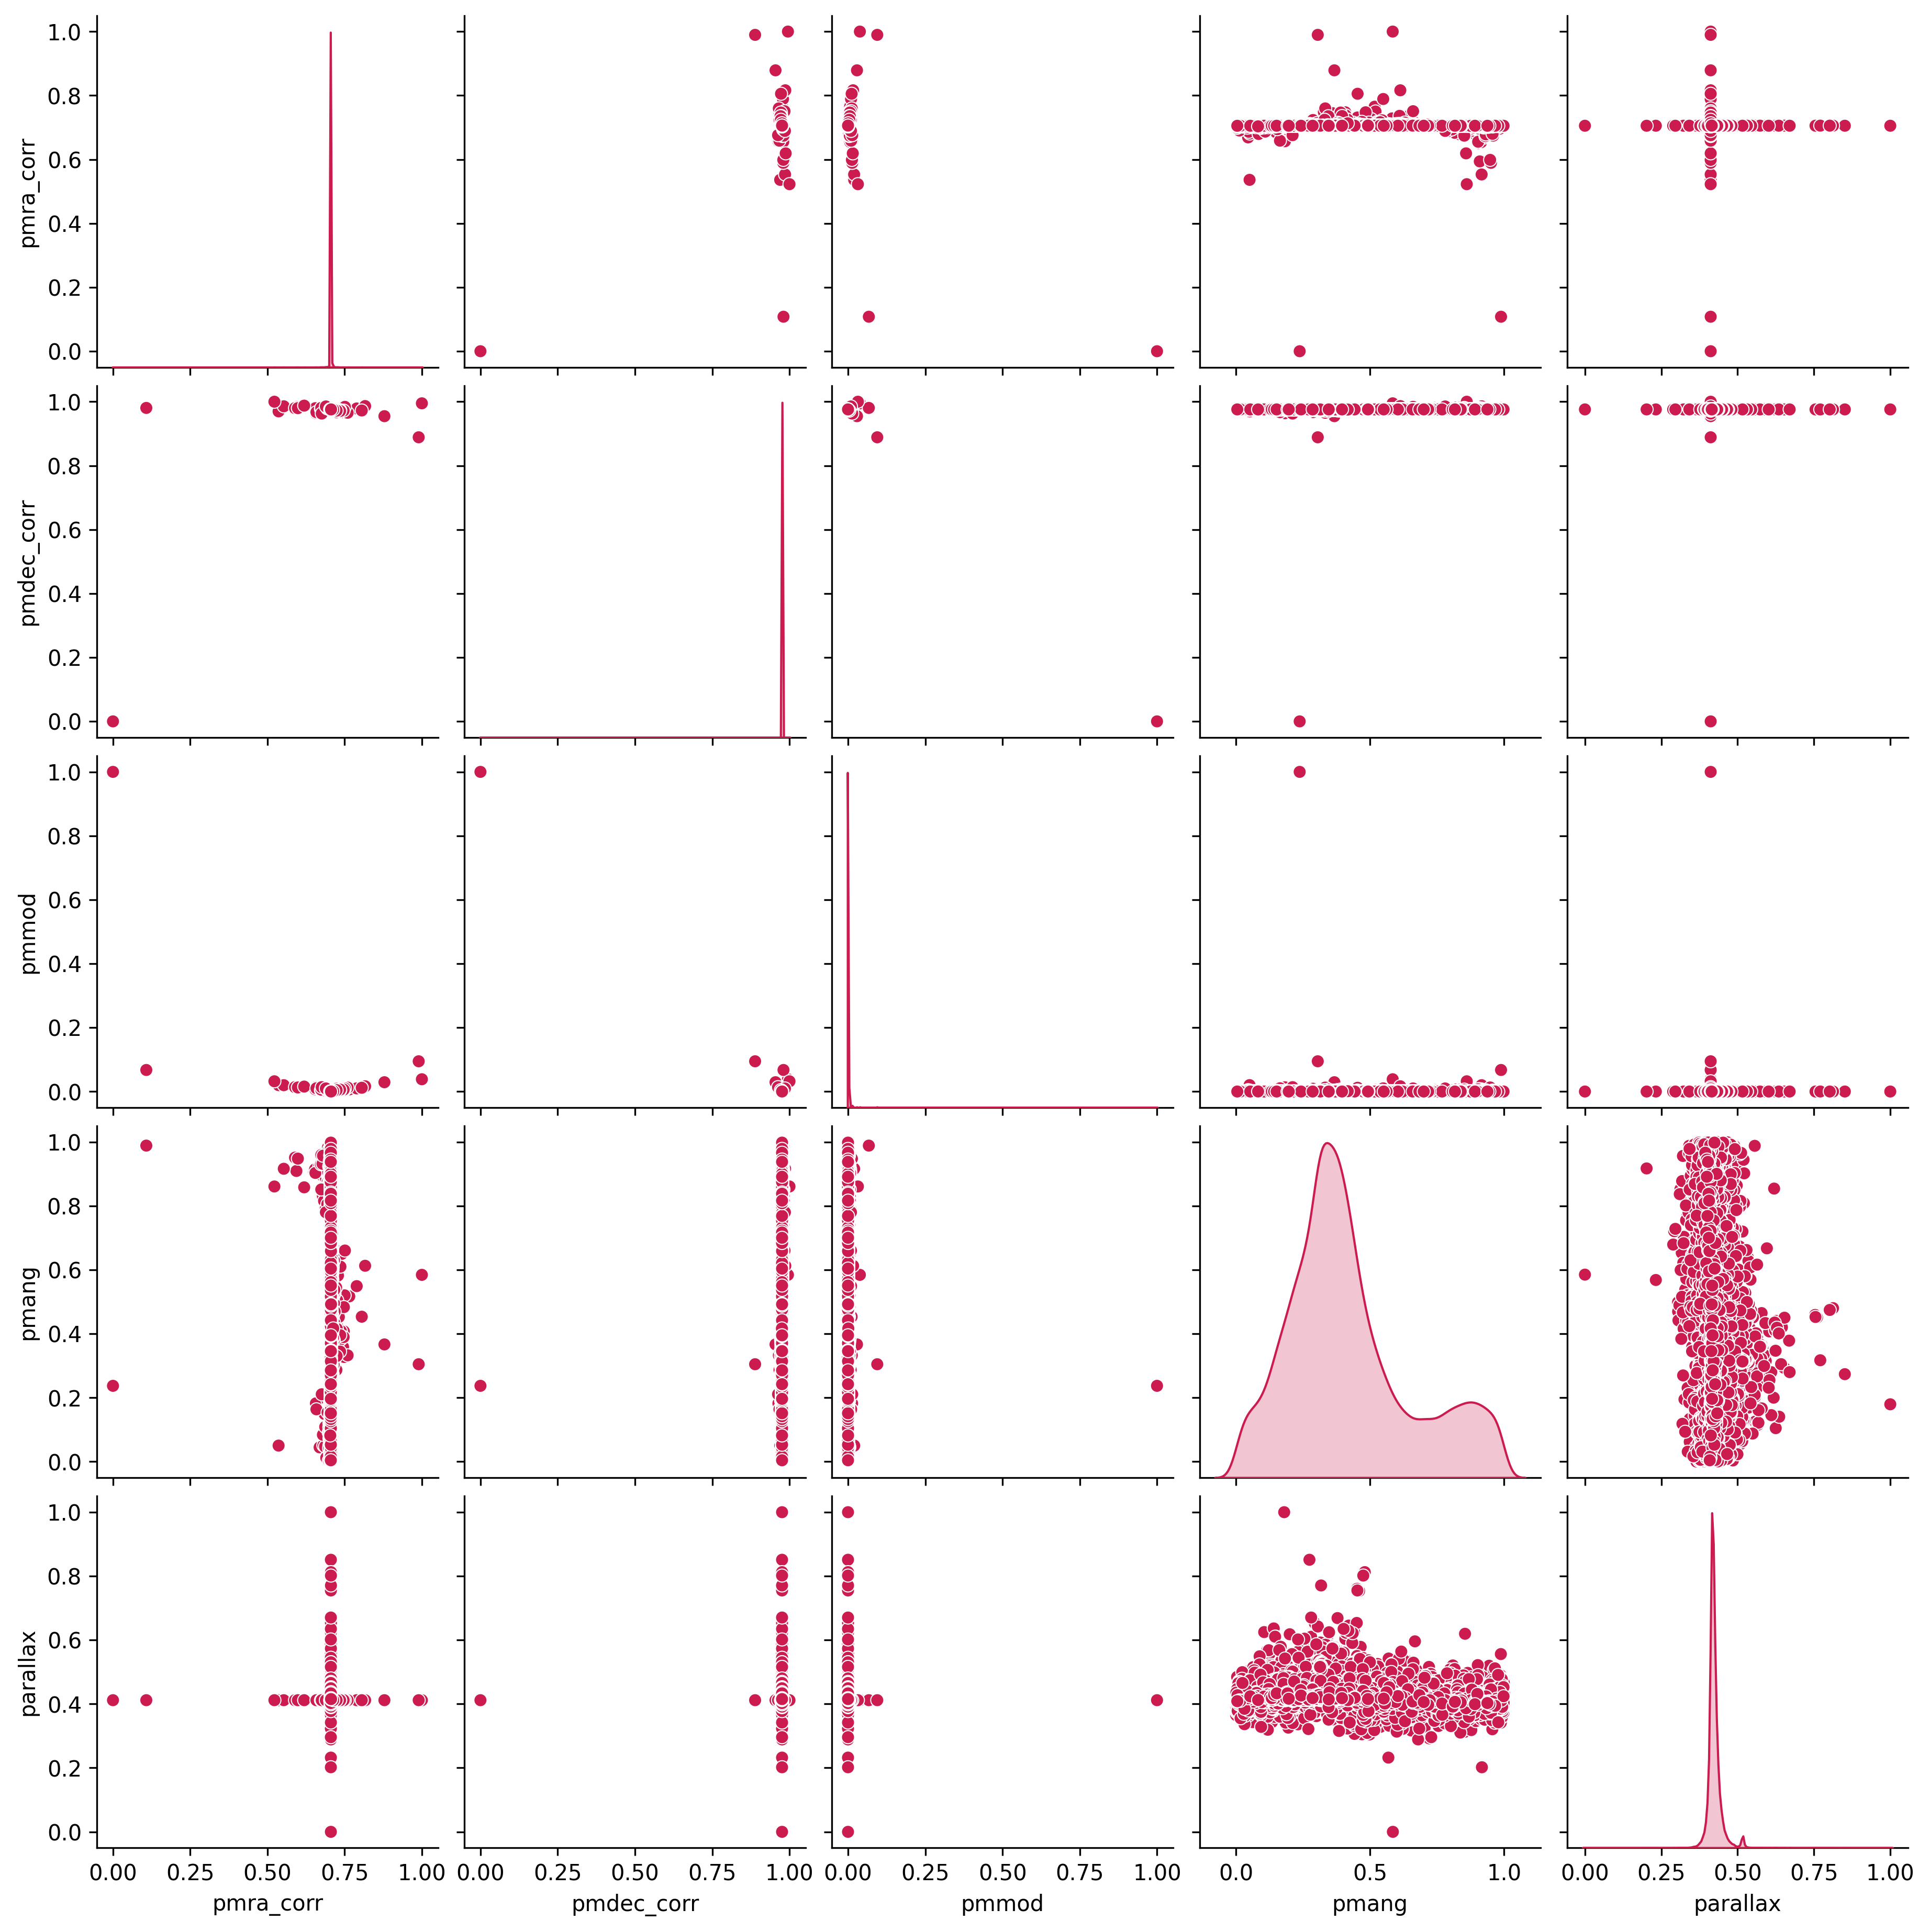
\includegraphics[width=\textwidth]{../figures/melotte_22/features_melotte_22.png}
  \end{subfigure}
  \caption{Pairwise relationships among variables using Melotte 22 data}
  \label{fig:features_melotte_22}
\end{figure}

\newpage

Figure~\ref{fig:features_melotte_22} shows a pairwise relationship among some features available
in the dataset for Melotte 22 data.
The diagonal of the grid shows the marginal distribution of the data in each column.
This plot can be useful to find correlations between pairs of variables or
to identify resonances in certain variables such as those in the parallax feature.

In summary, these are the features we are going to use as sources for our clustering models:

\begin{itemize}
  \item \emph{Proper motion in right ascension} (corrected by parallax): \(\mu_{\alpha}\)
  \item \emph{Proper motion in declination} (corrected by parallax): \(\mu_{\delta}\)
  \item \emph{Parallax}: \( \varpi \)
  \item \emph{Proper motion modulus}: \(\left\| \vec{\mu} \right\|\)
\end{itemize}

This feature selection has been refined by iterating over the K-Means clustering process
with a fixed number of clusters and varying the feature selection in each case.
The final selection is the one with best \emph{silhouette score}~\cite{rousseeuw1987silhouettes}.

The silhouette score is a metric used to determine how good a cluster is based on intra-cluster
distances and nearest-cluster distances. The best possible value is 1, and the worst is -1.
Negative values mean that some samples have been assigned to the wrong cluster.

\section{Soft Clustering with K-Means}

Once we have found the set of features that best describes our problem,
we can begin searching for the OC within the selected region.

Our first approach to find the open cluster is using the K-Means algorithm.

Since we are looking for a single cluster,
it seems reasonable to use a clustering algorithm and set it to find two clusters.
One for the desired OC and another which contains stars that do not belong to the open cluster.
However, this idea is not completely right.

\begin{figure}[htbp]
  \centering
  \begin{subfigure}{0.9\textwidth}
    \centering
    \begin{subfigure}[t]{0.3\textwidth}
      \centering
      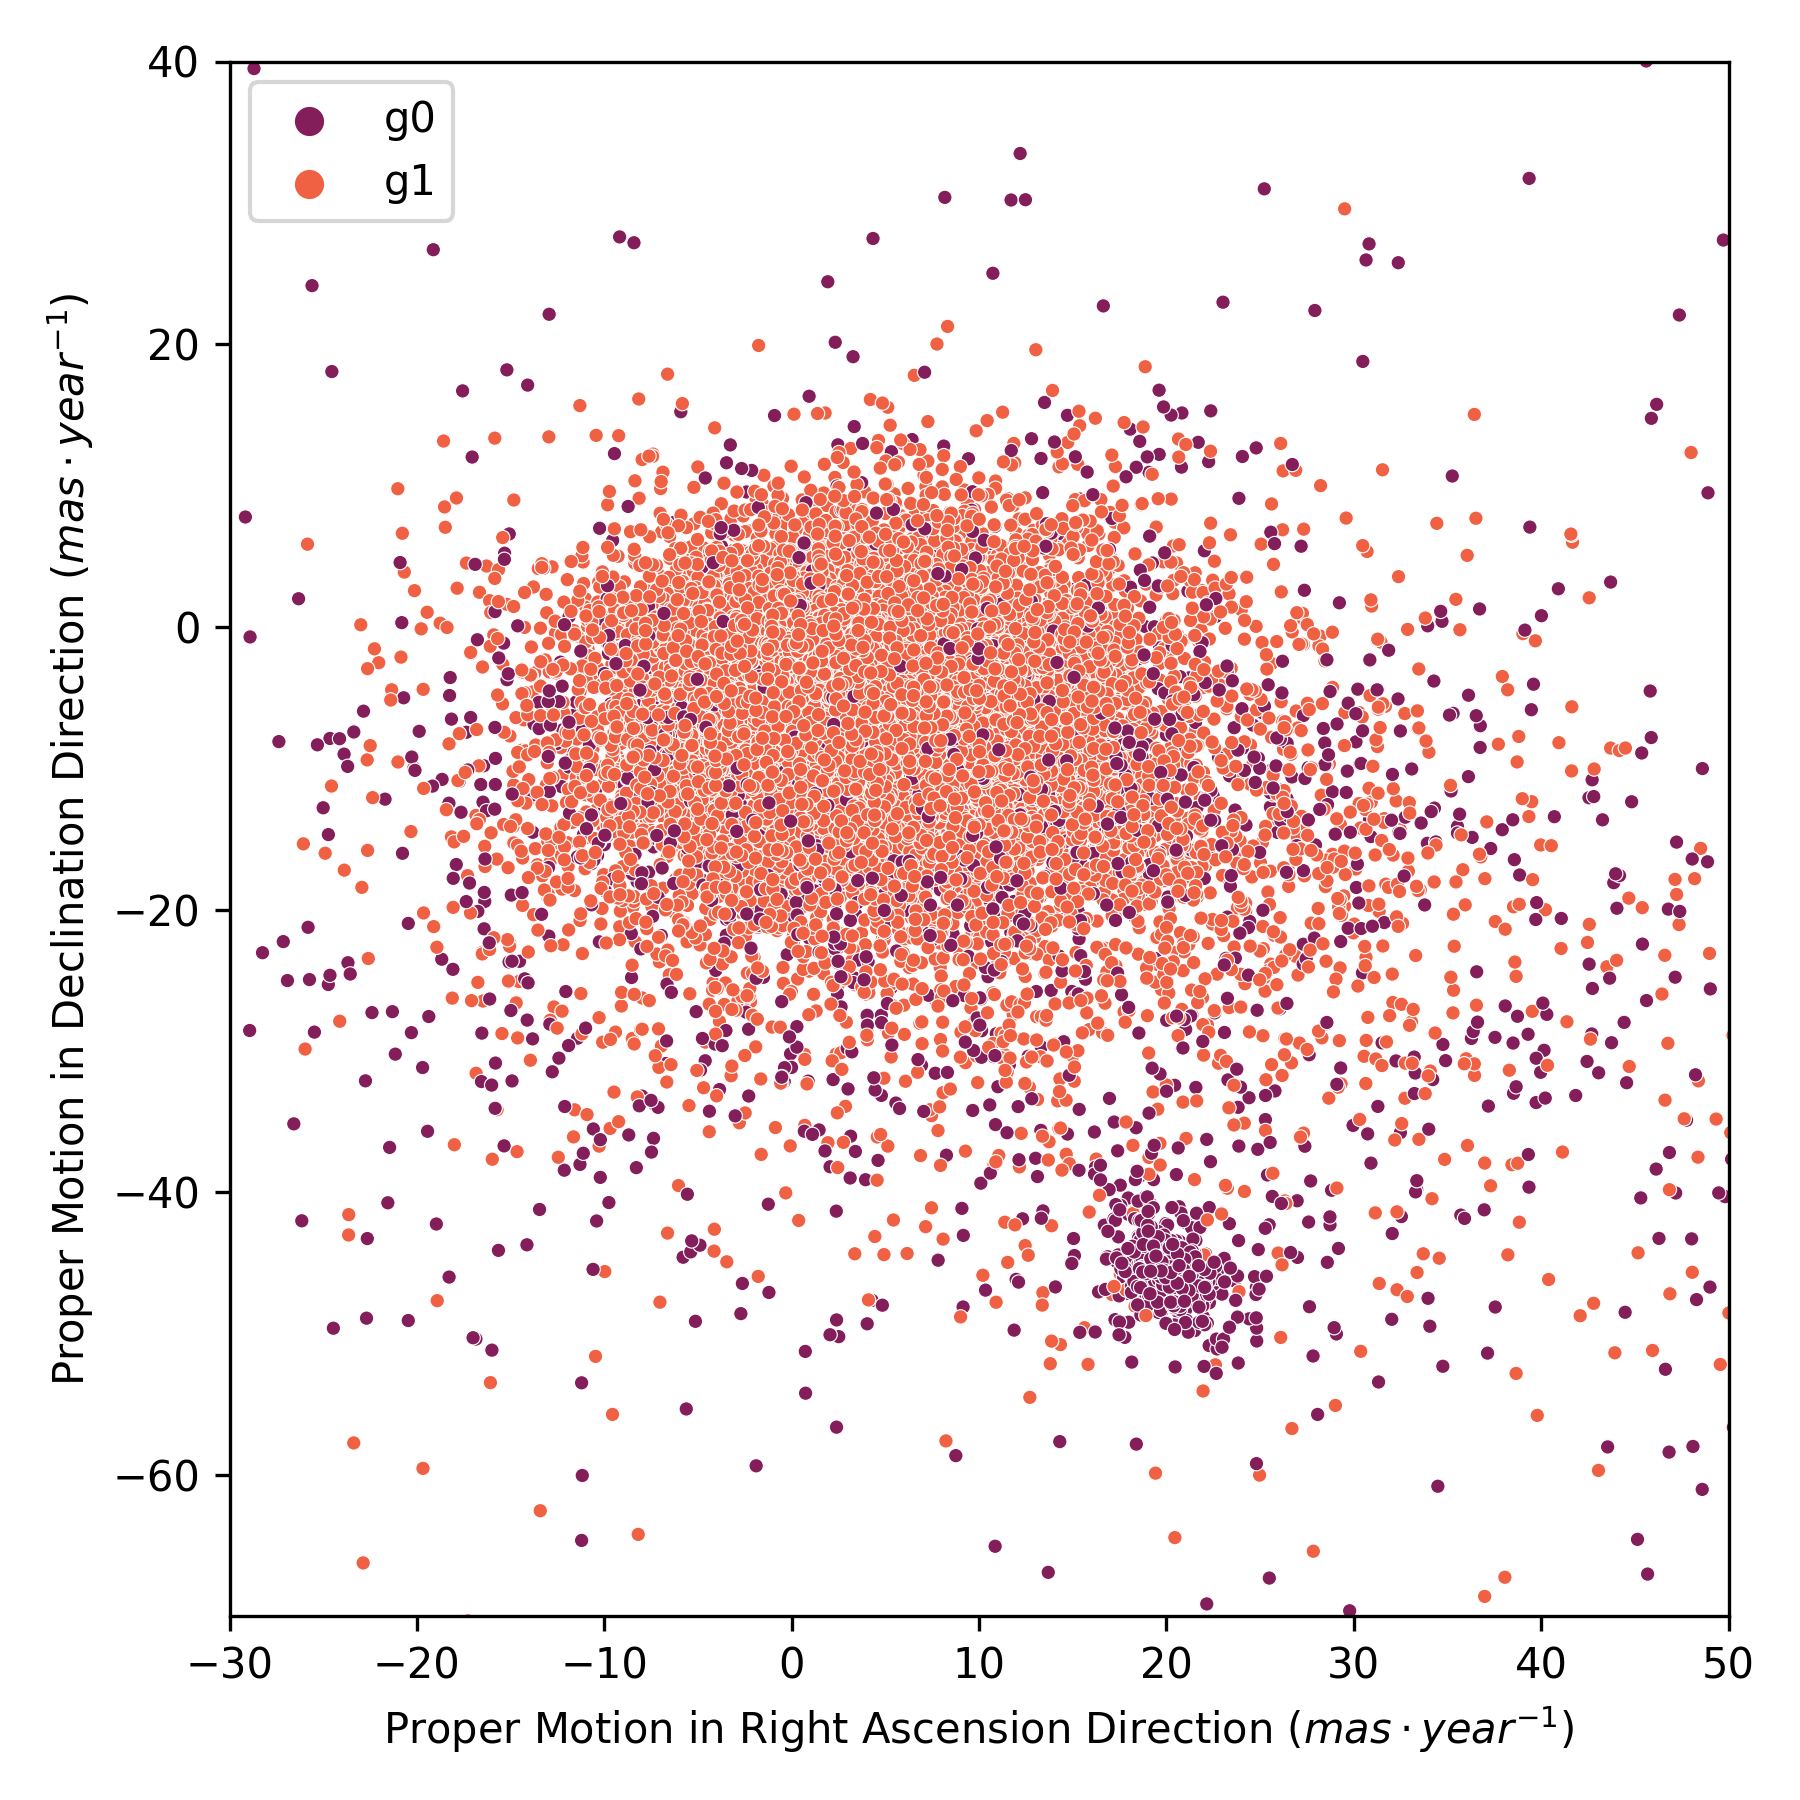
\includegraphics[width=\textwidth]{../figures/kmeans/kmeans_n2_pm_melotte_22.png}
    \end{subfigure}
    \hfill
    \begin{subfigure}[t]{0.3\textwidth}
      \centering
      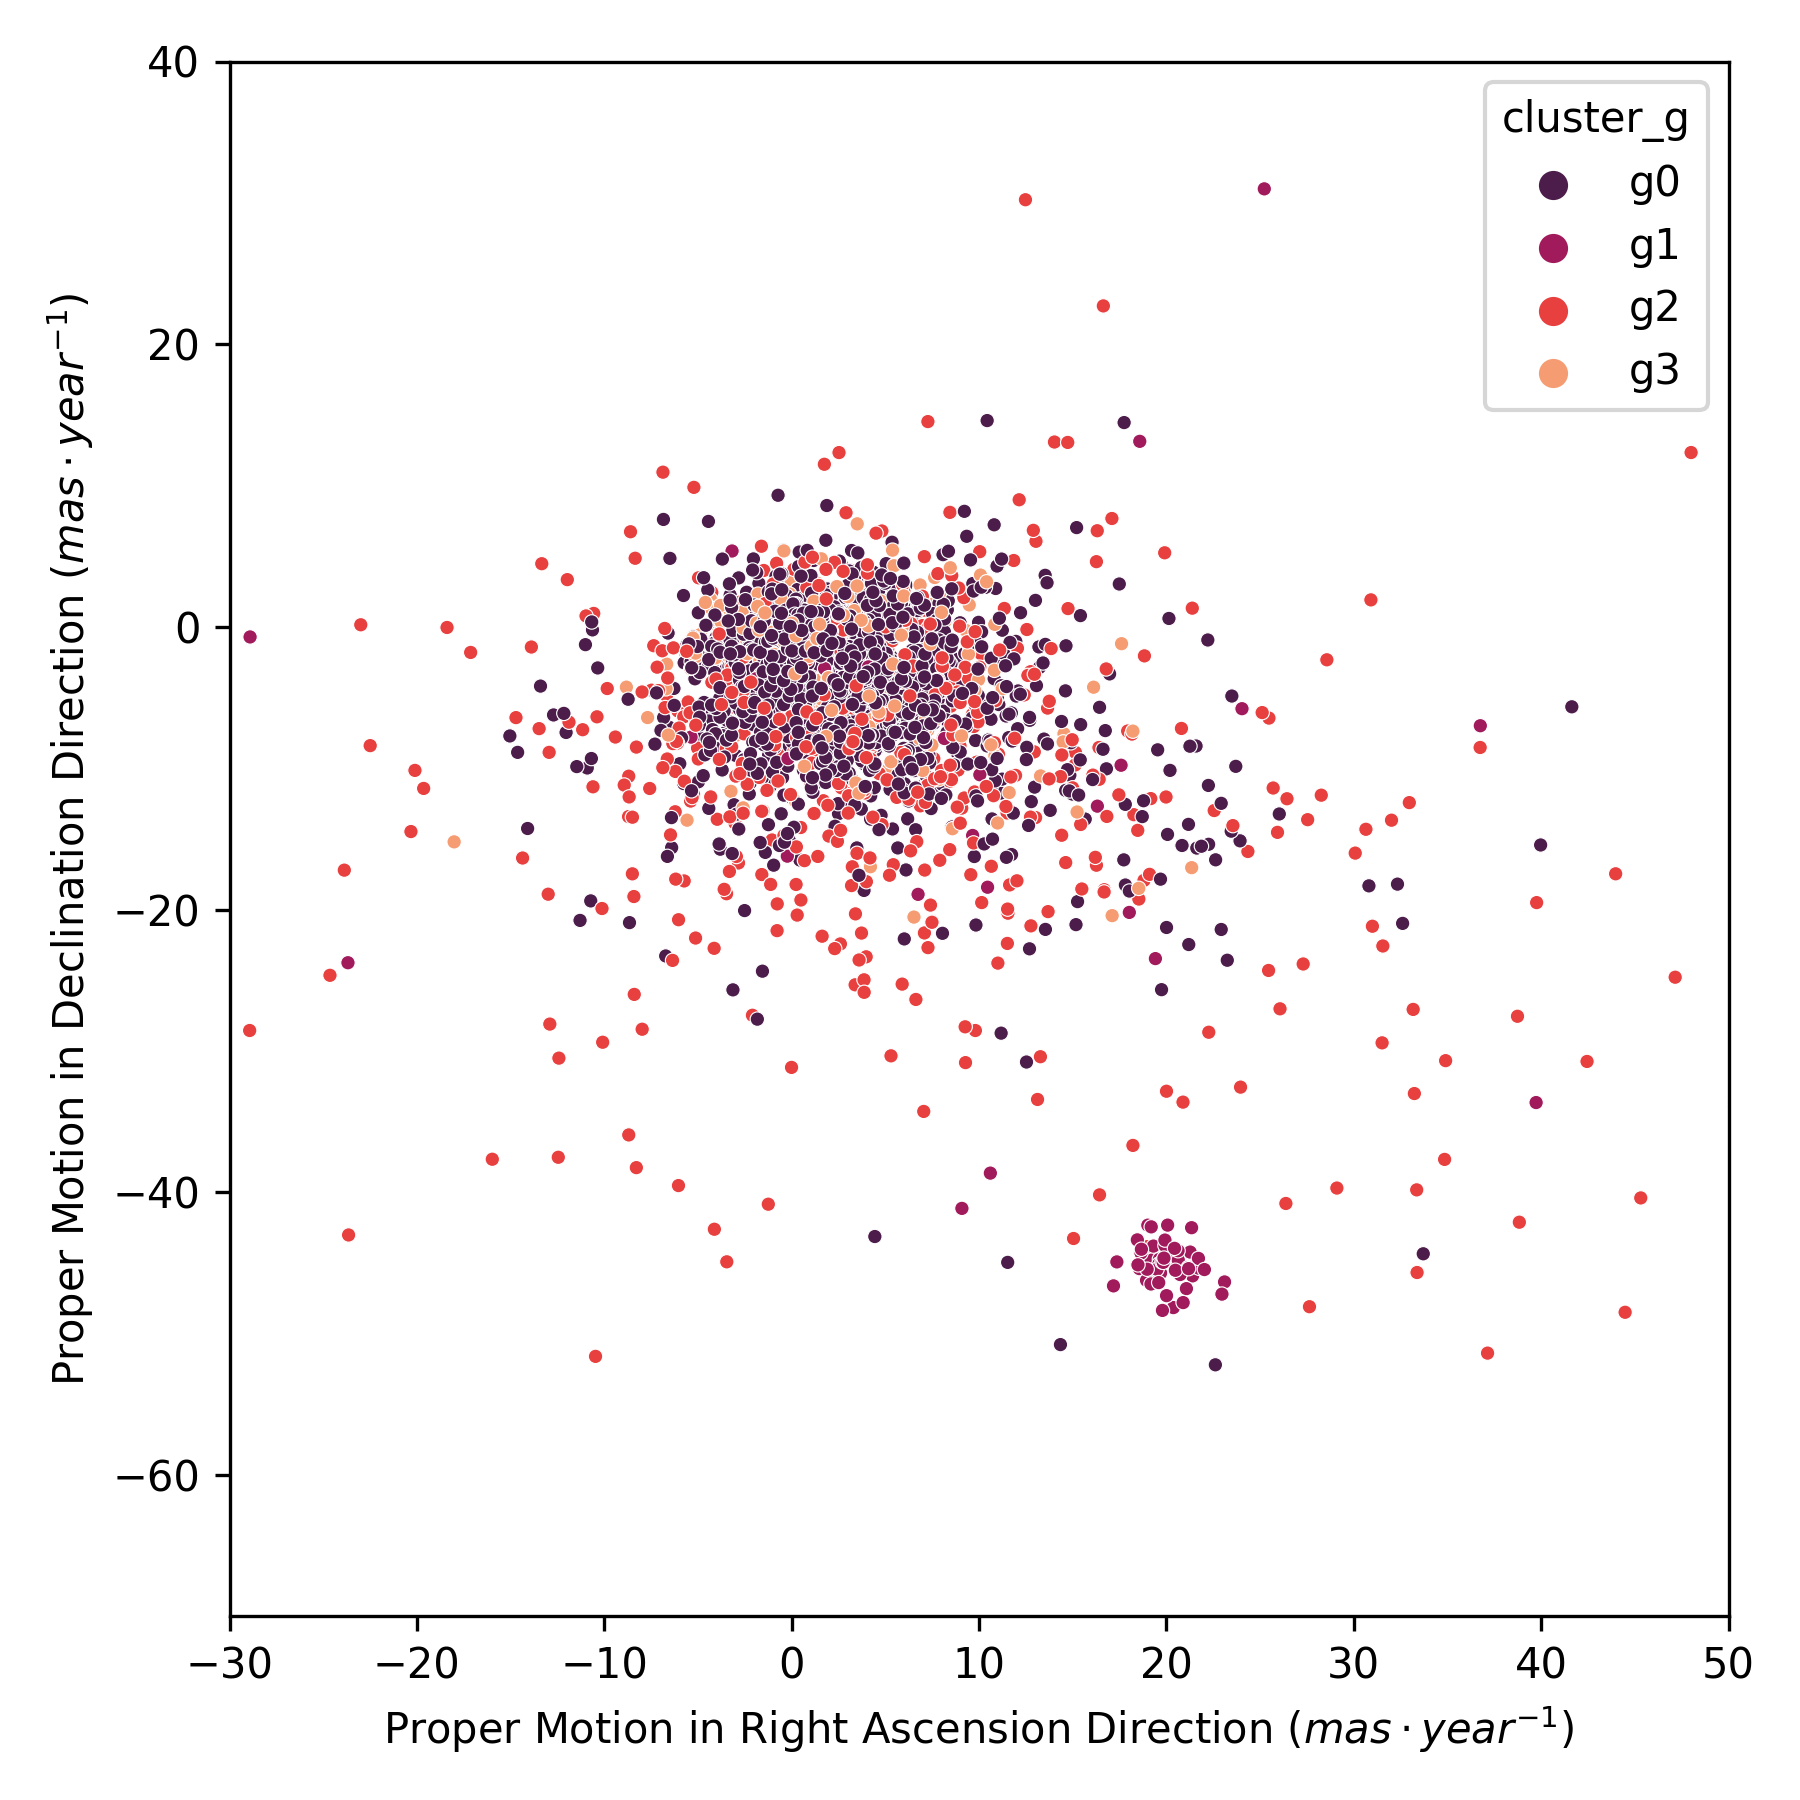
\includegraphics[width=\textwidth]{../figures/kmeans/kmeans_n5_pm_melotte_22.png}
    \end{subfigure}
    \hfill
    \begin{subfigure}[t]{0.3\textwidth}
      \centering
      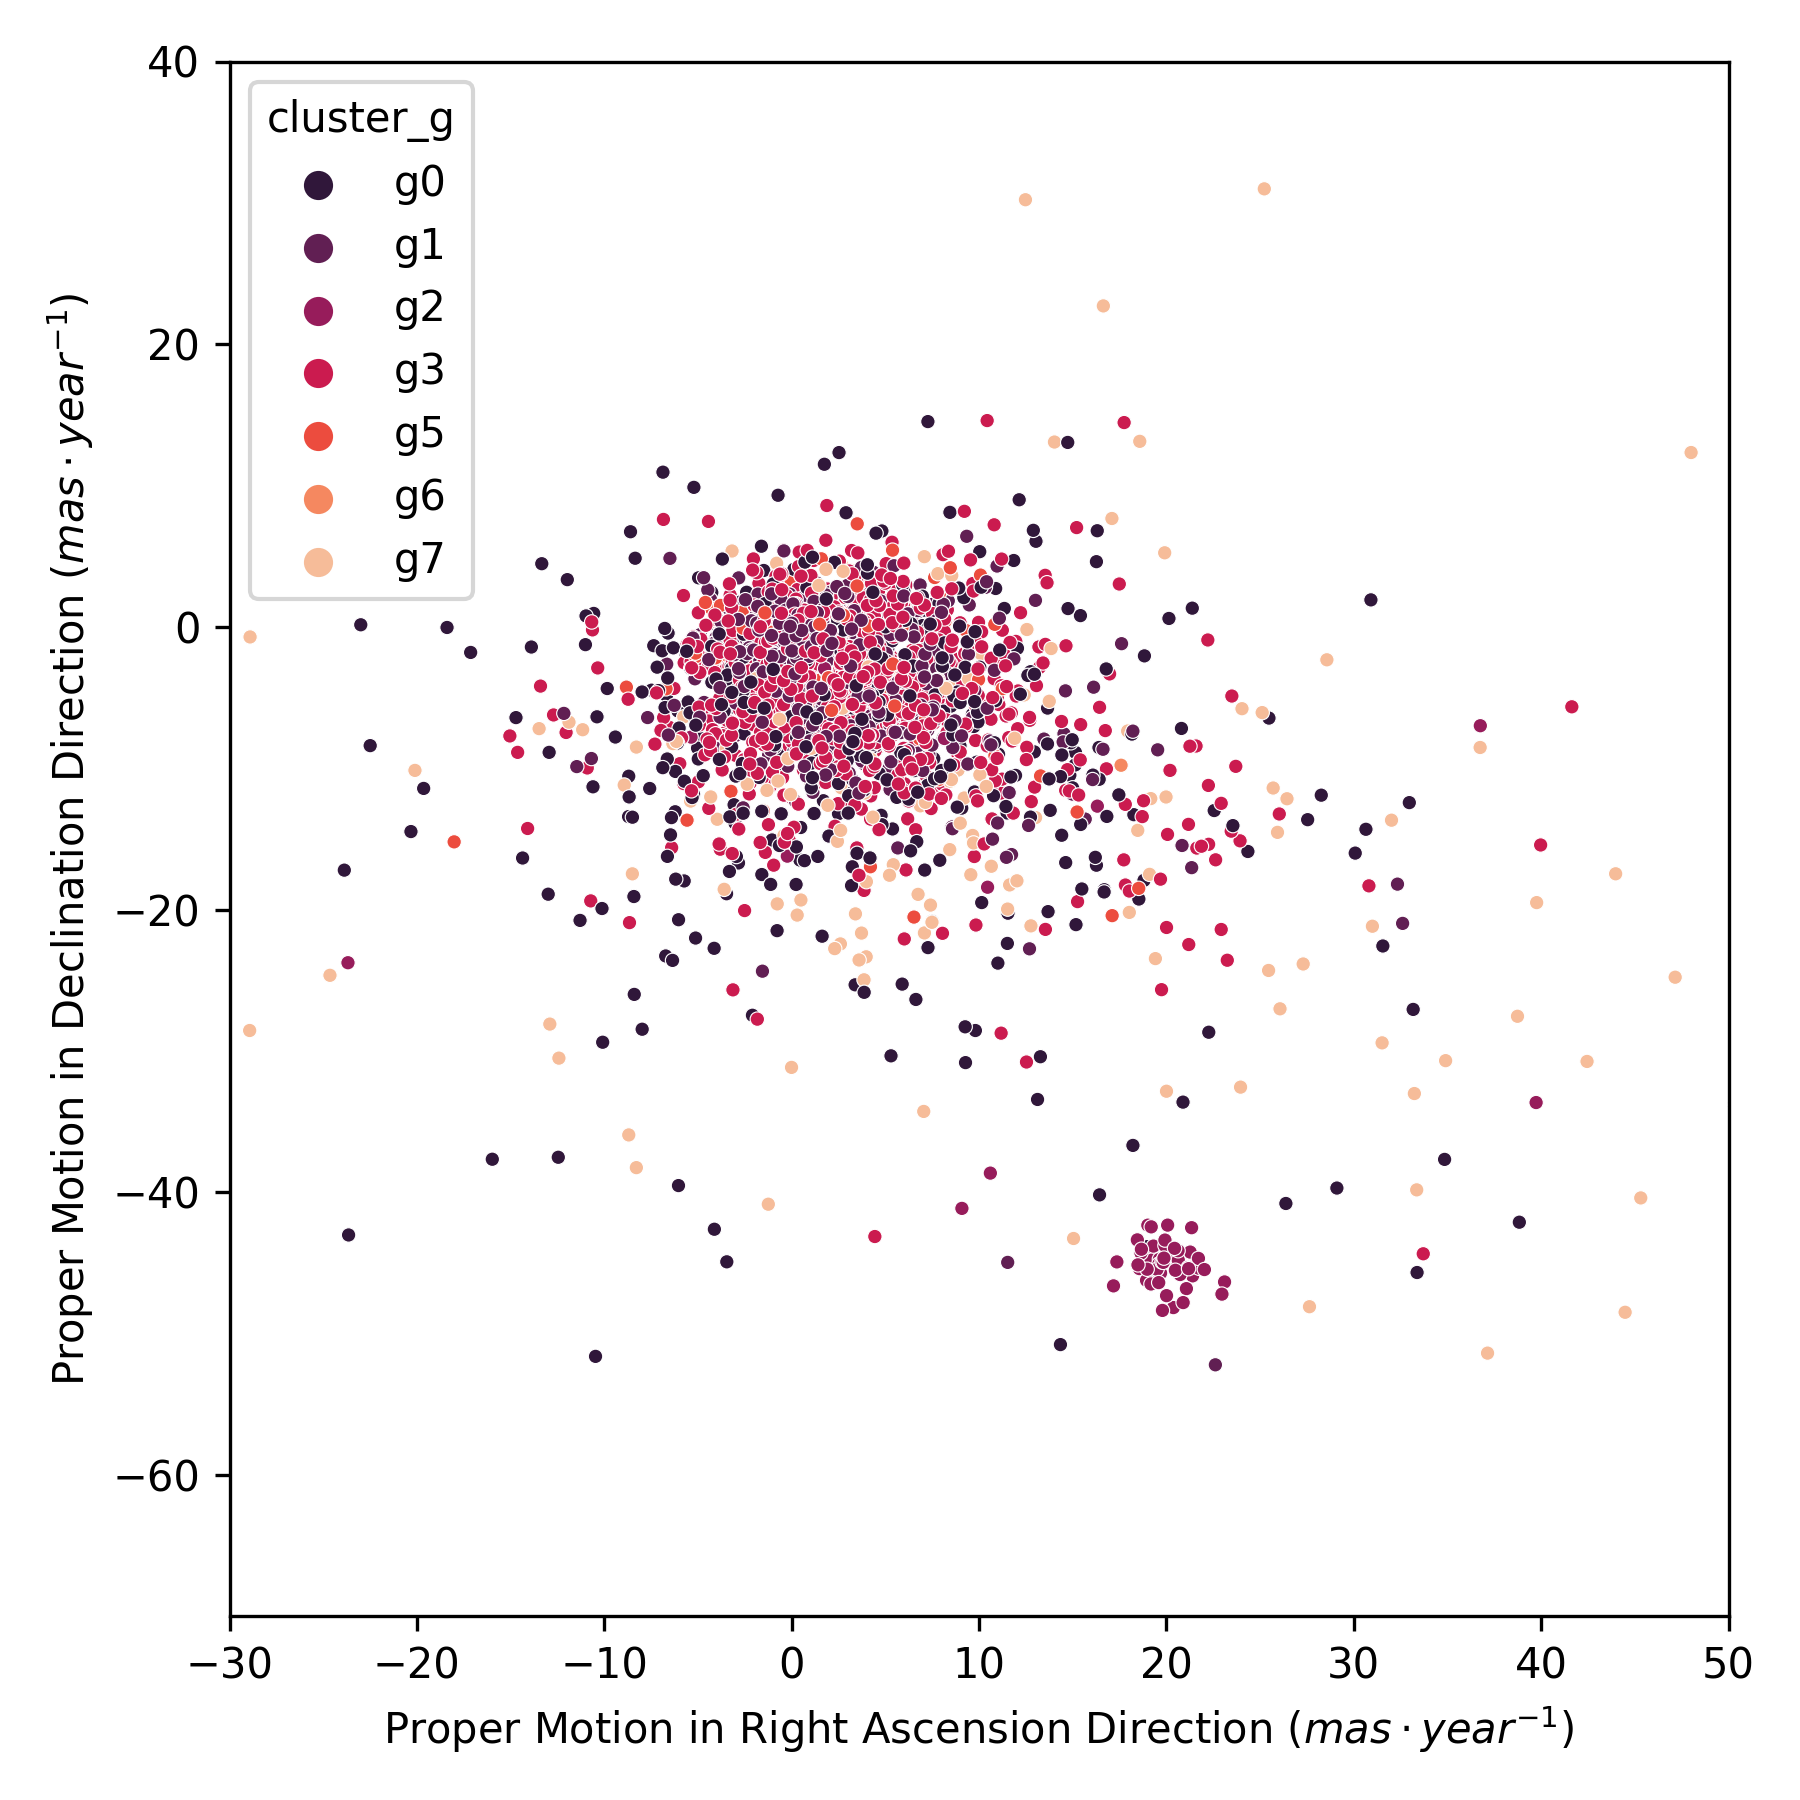
\includegraphics[width=\textwidth]{../figures/kmeans/kmeans_n8_pm_melotte_22.png}
    \end{subfigure}
  \end{subfigure}
  \medskip
  \begin{subfigure}{0.9\textwidth}
    \centering
    \begin{subfigure}[t]{0.3\textwidth}
      \centering
      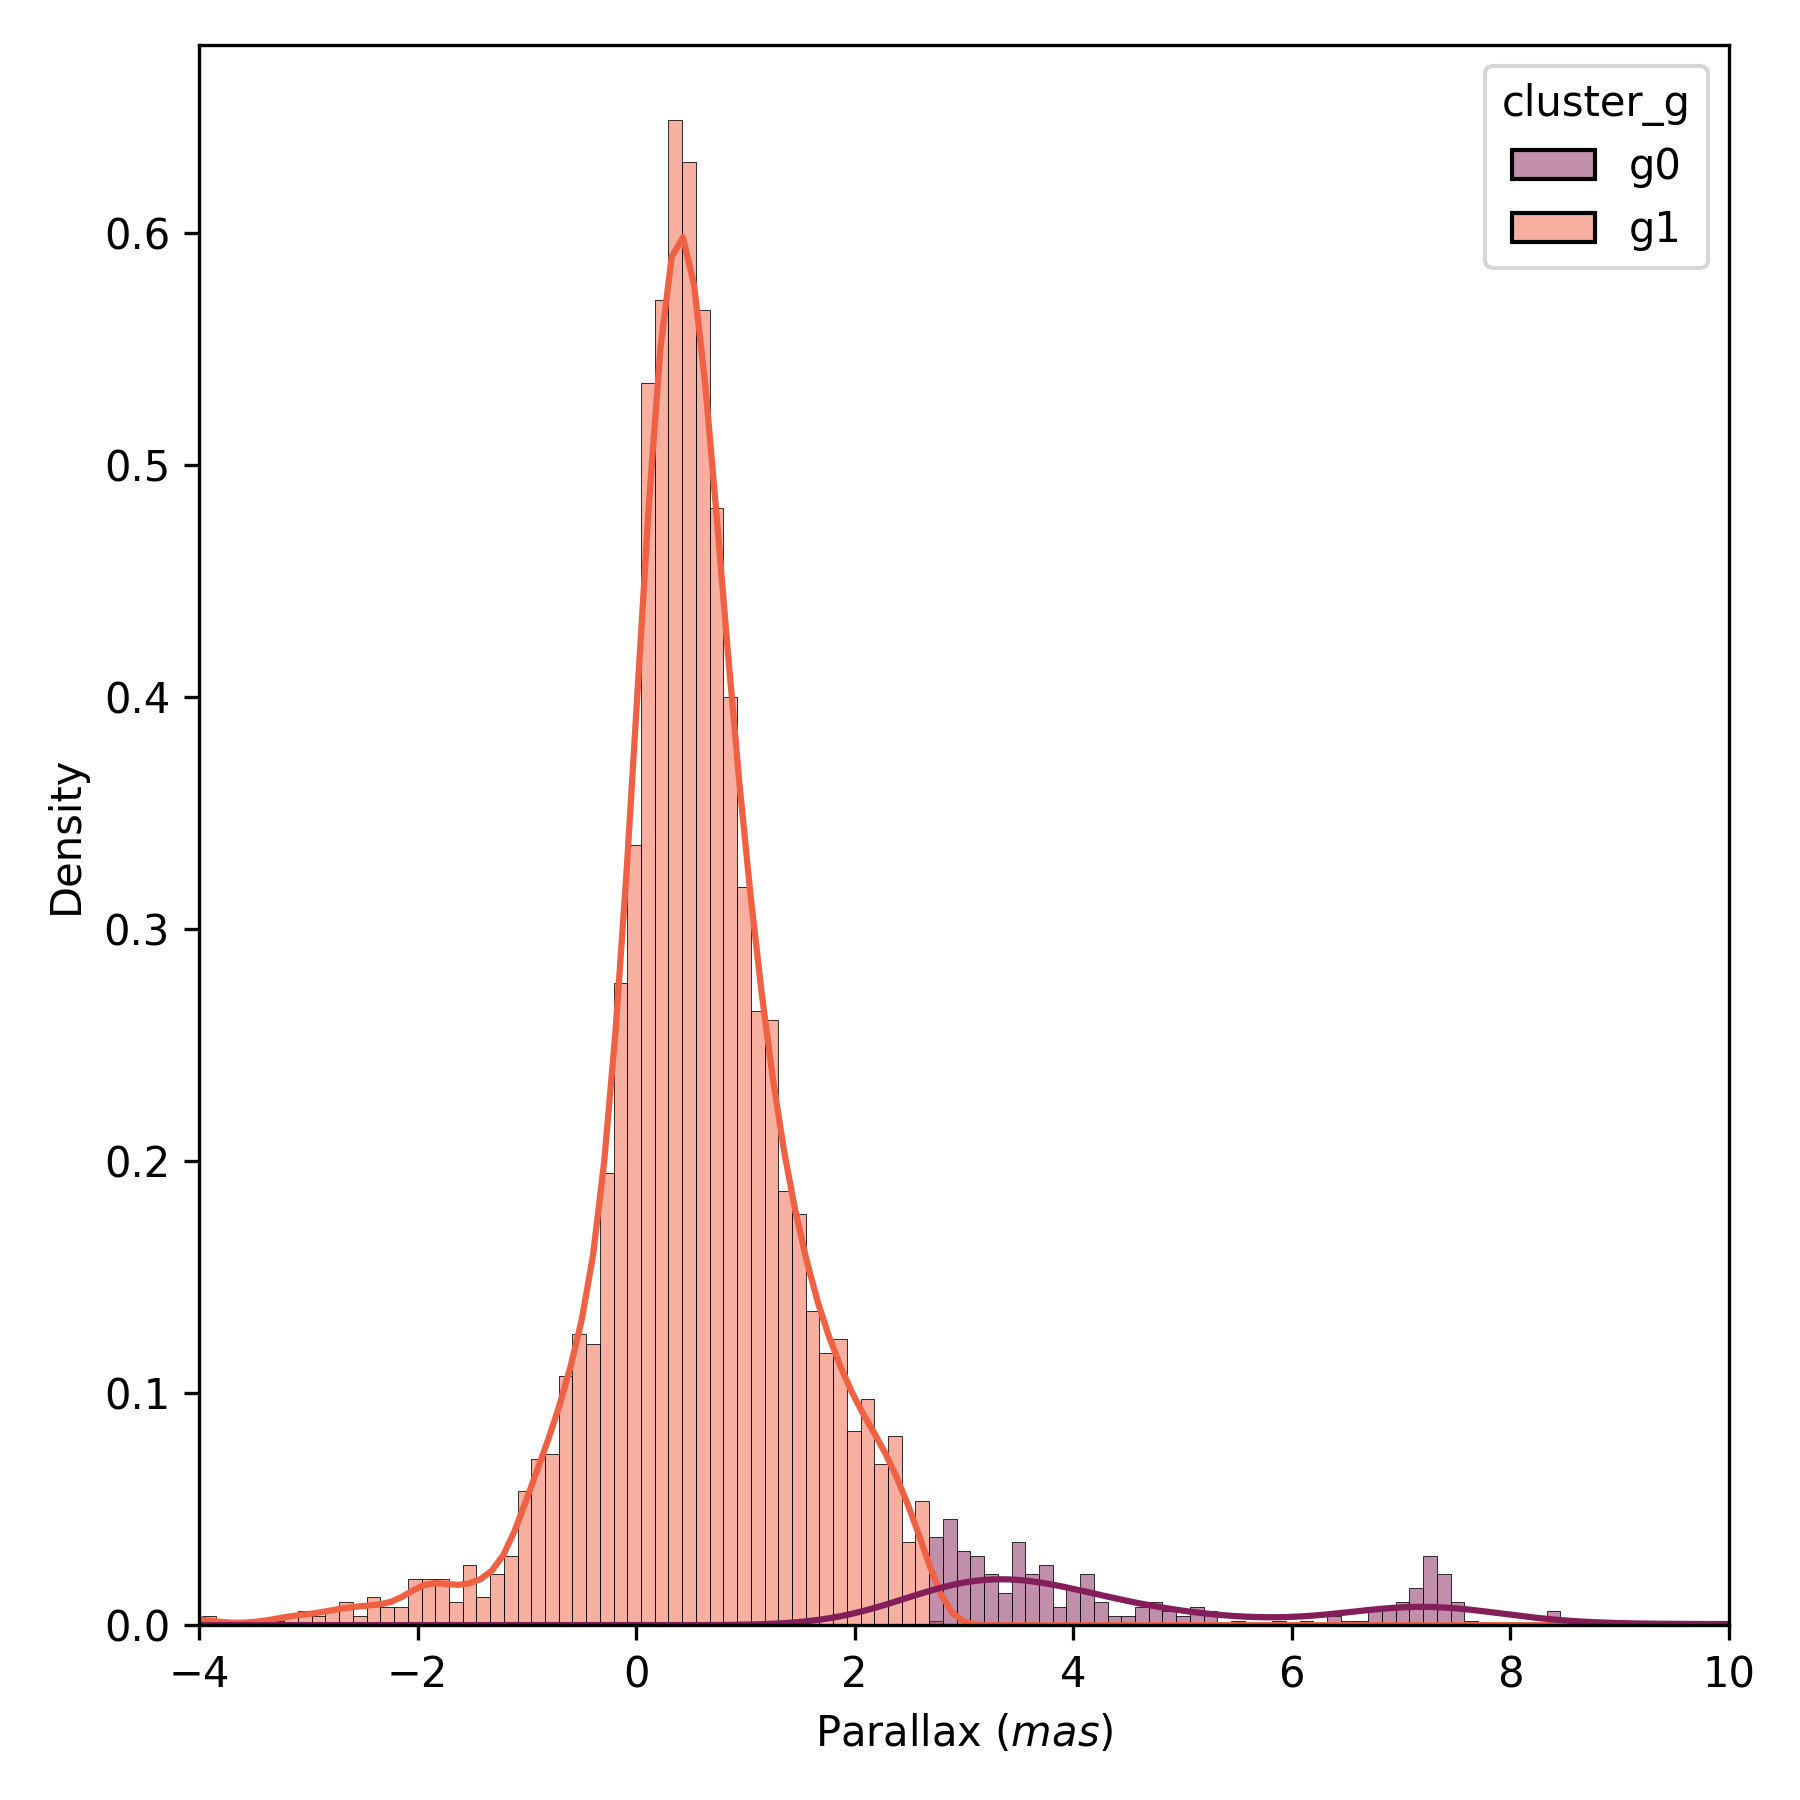
\includegraphics[width=\textwidth]{../figures/kmeans/kmeans_n2_parallax_melotte_22.png}
      \caption{N clusters = 2}
    \end{subfigure}
    \hfill
    \begin{subfigure}[t]{0.3\textwidth}
      \centering
      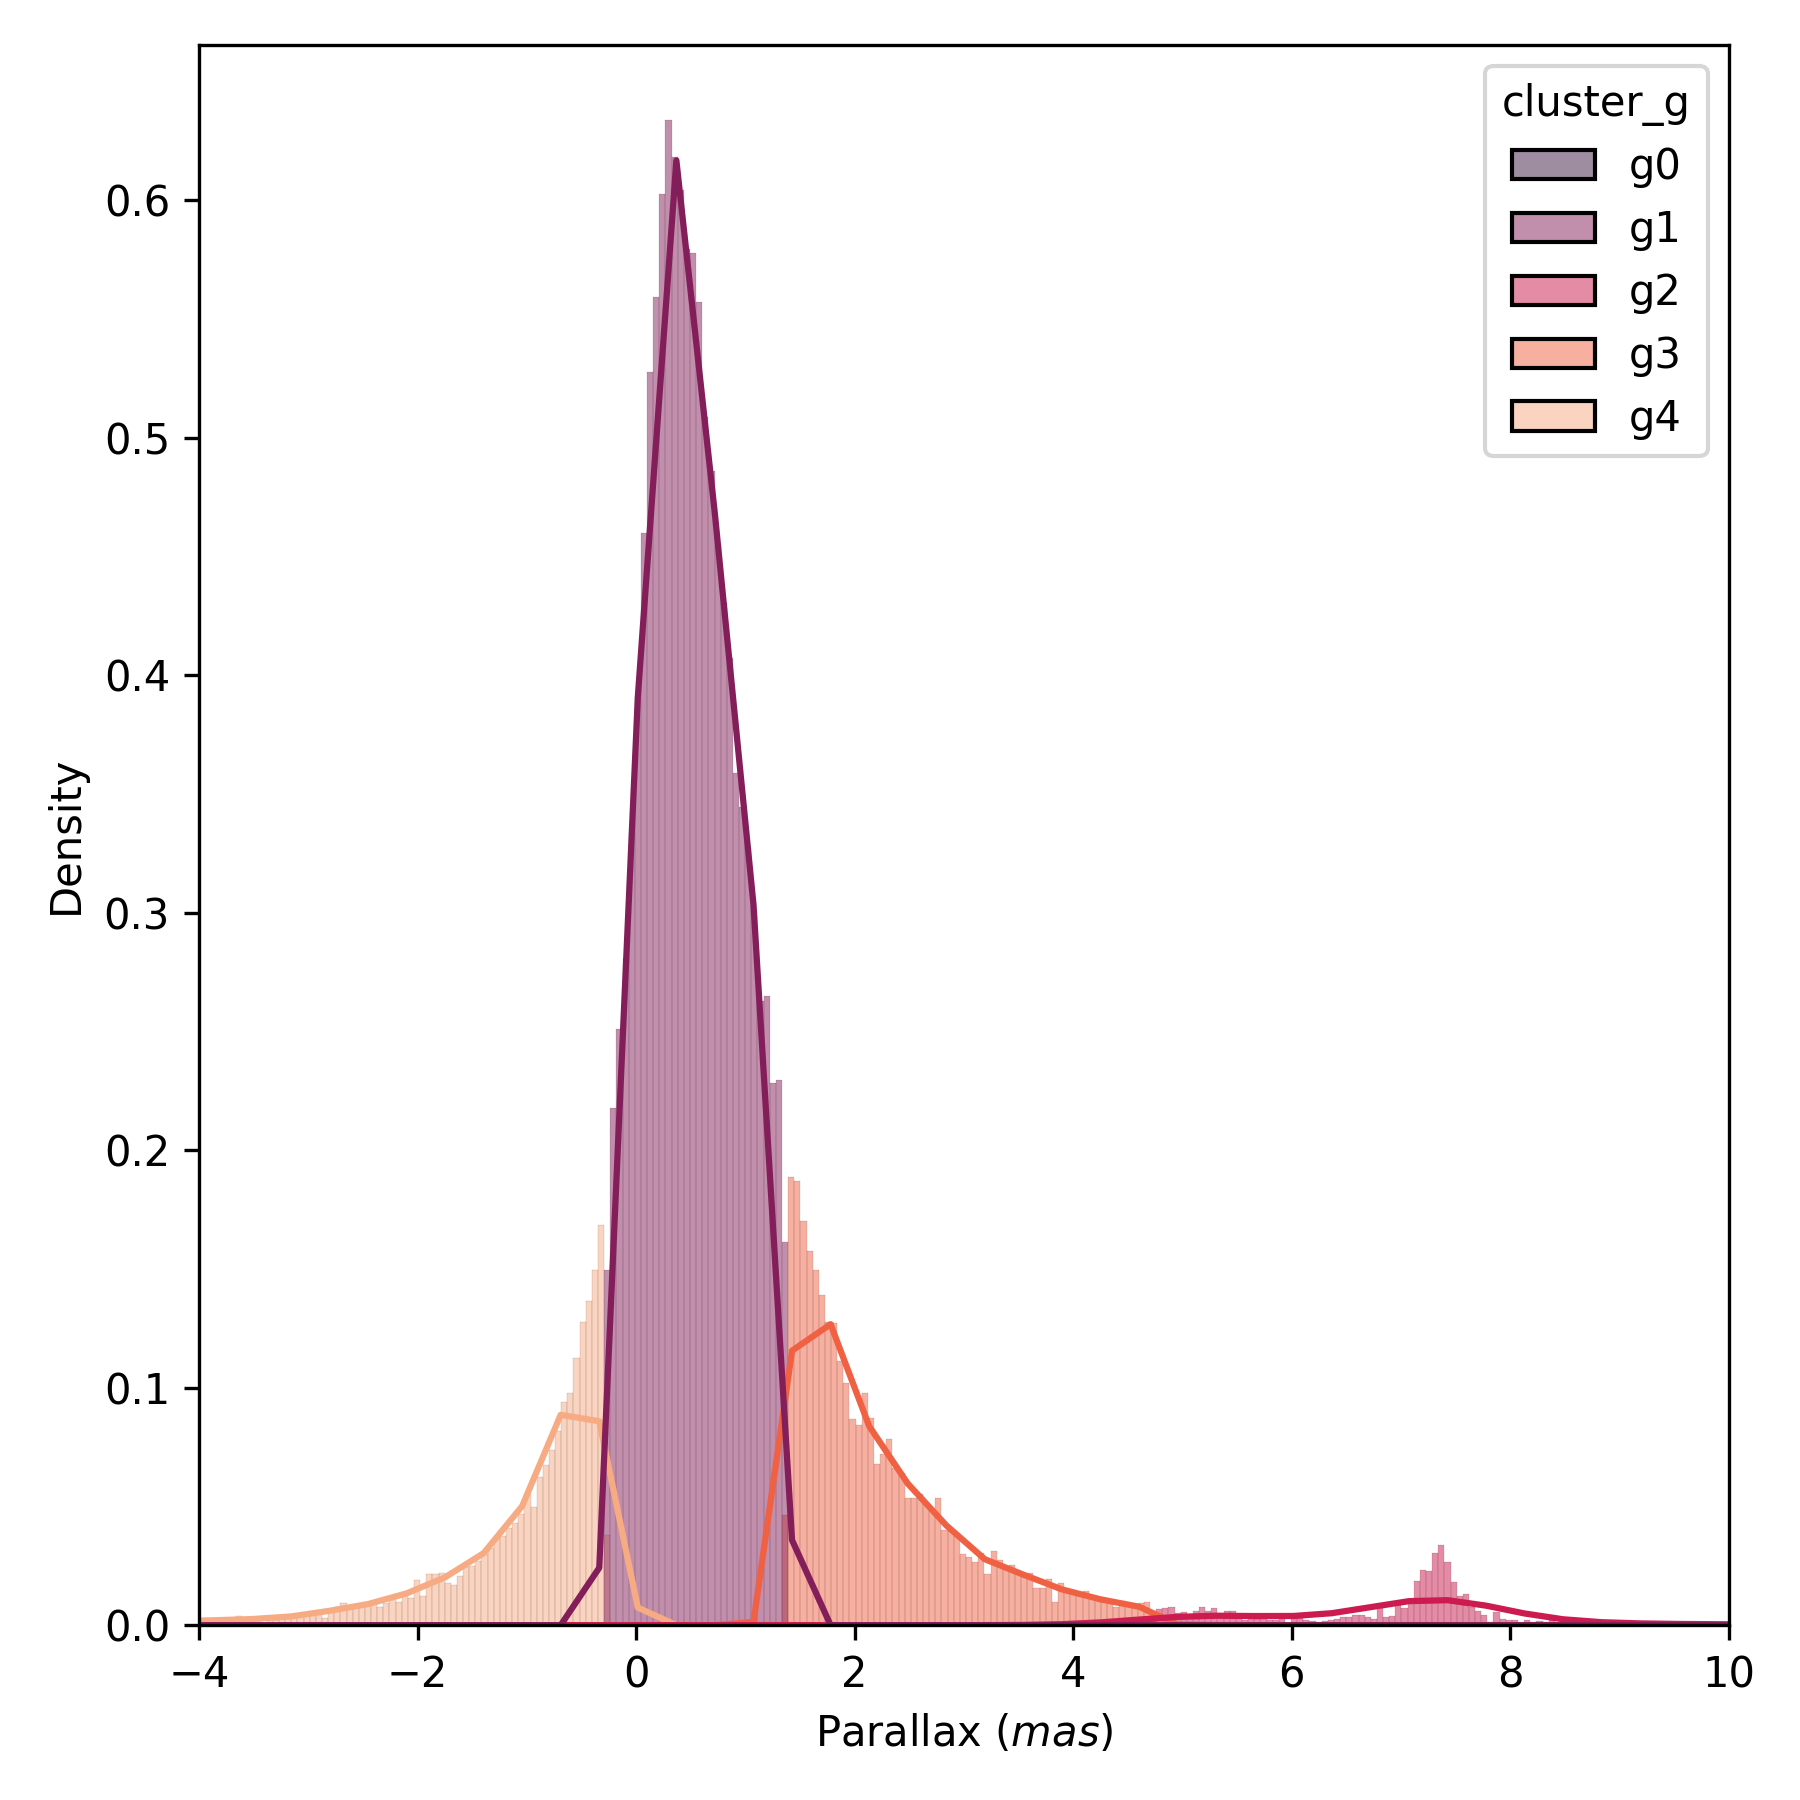
\includegraphics[width=\textwidth]{../figures/kmeans/kmeans_n5_parallax_melotte_22.png}
      \caption{N clusters = 5}
    \end{subfigure}
    \hfill
    \begin{subfigure}[t]{0.3\textwidth}
      \centering
      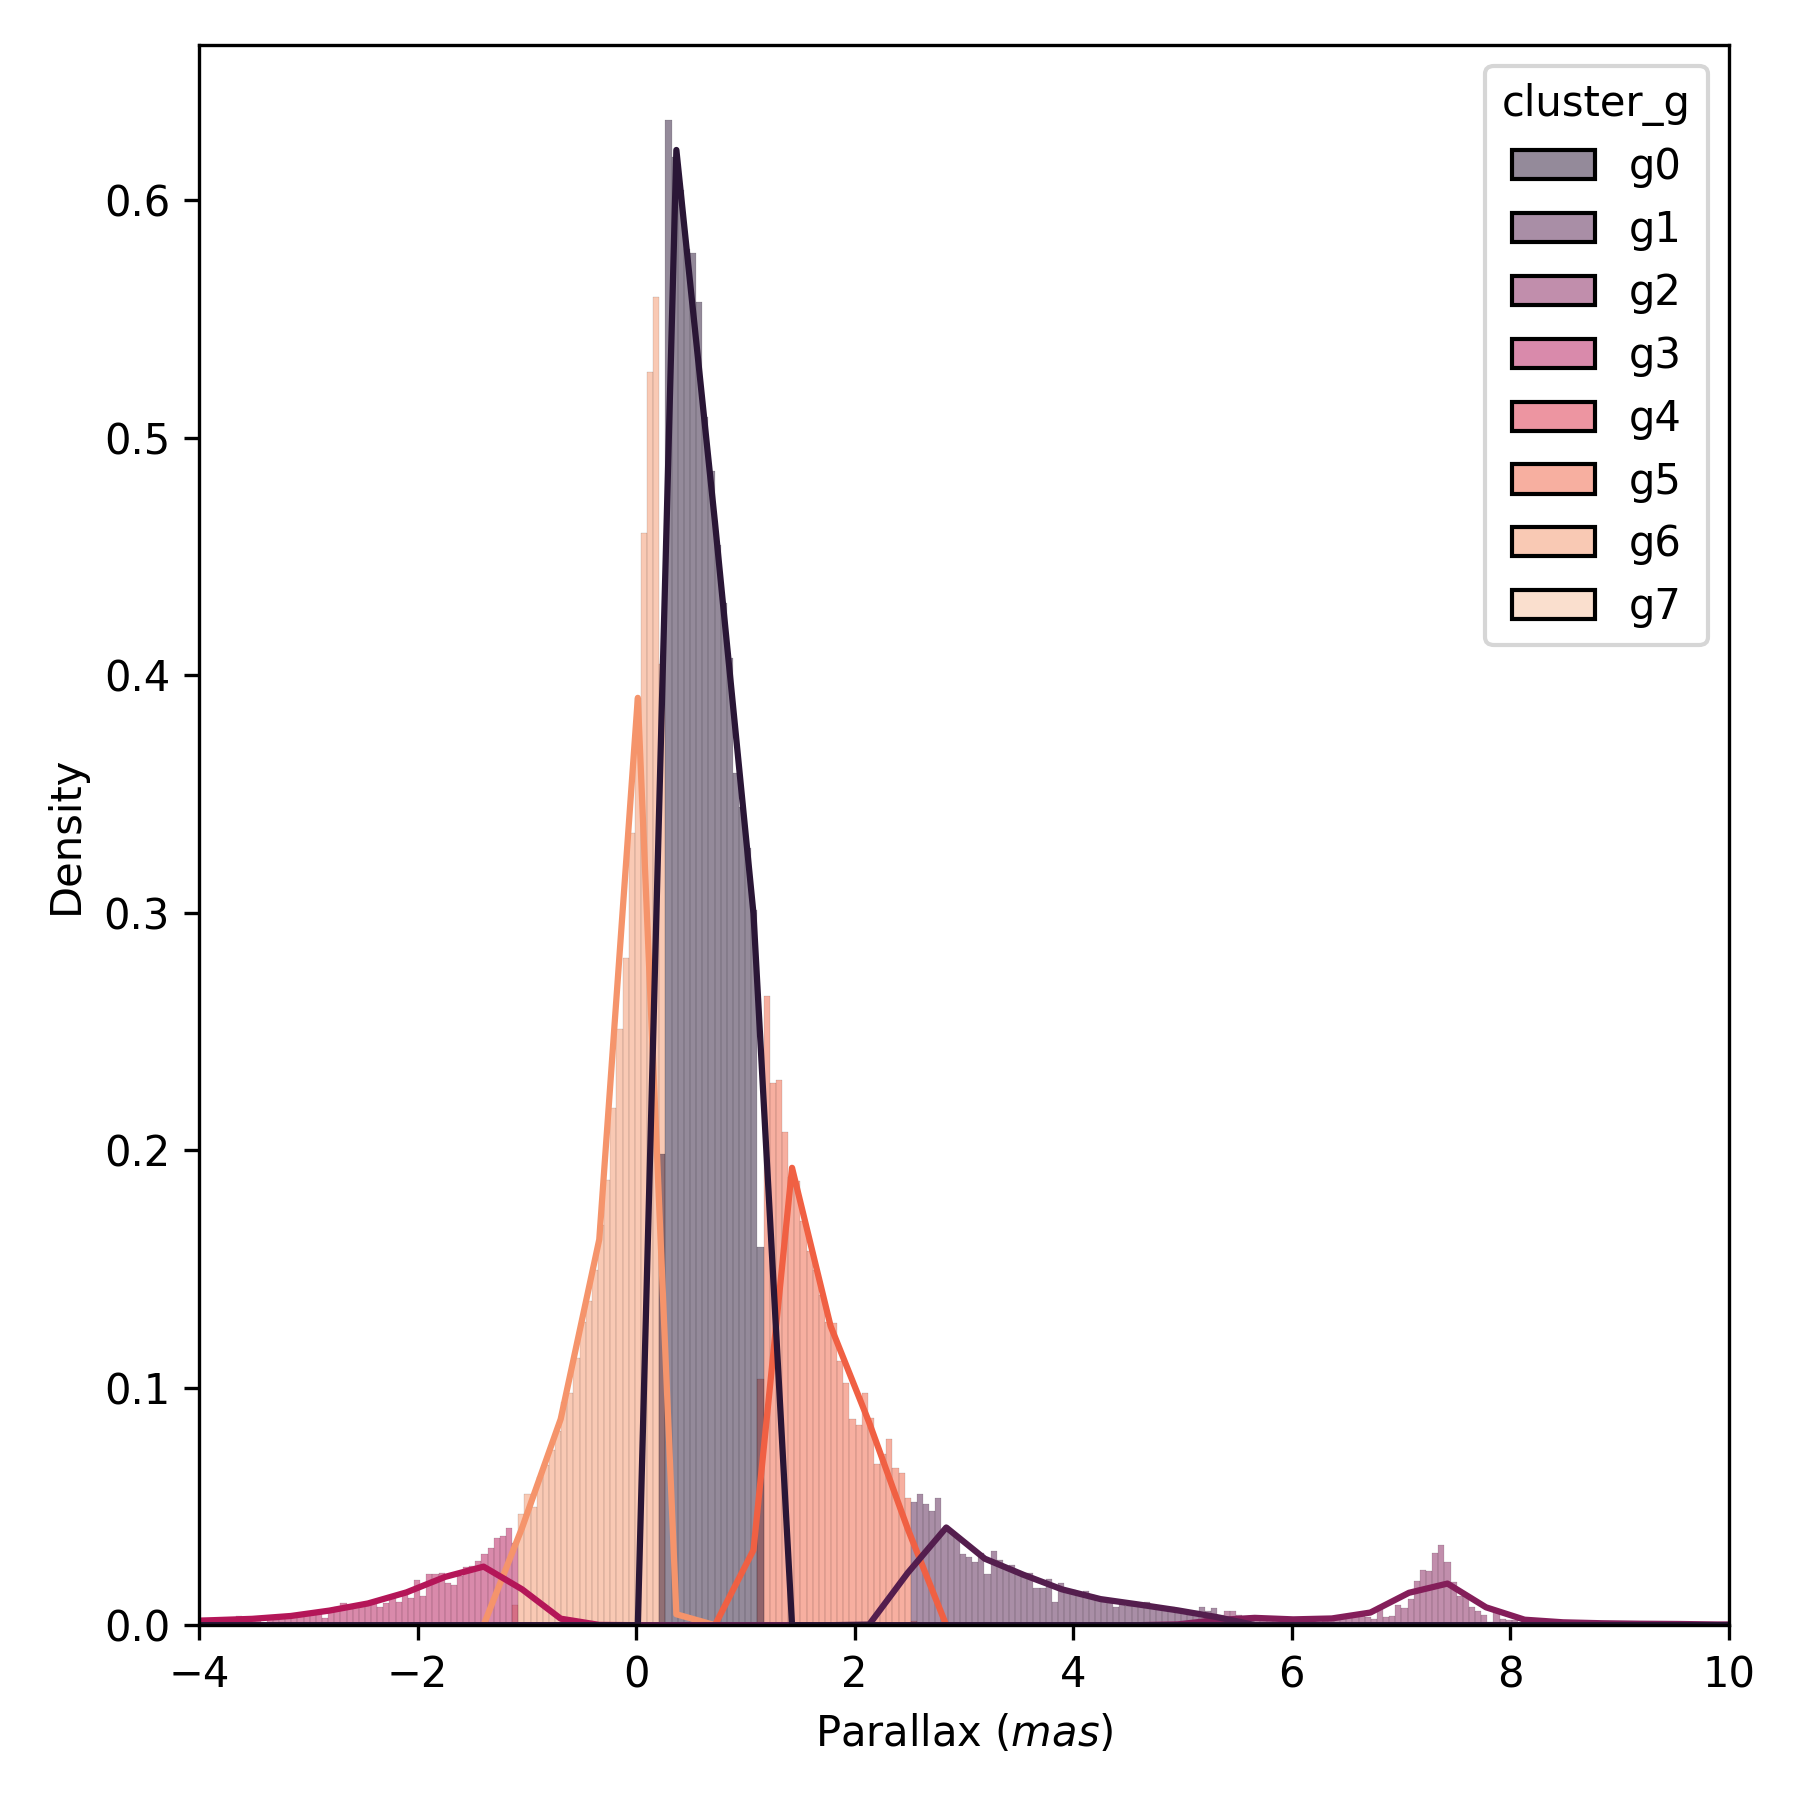
\includegraphics[width=\textwidth]{../figures/kmeans/kmeans_n8_parallax_melotte_22.png}
      \caption{N clusters = 8}
    \end{subfigure}
  \end{subfigure}
  \caption{K-Means comparisons with Melotte 22}
  \label{fig:kmeans_comparisons_melotte_22}
\end{figure}

This is due to the fact that OC's stars are surrounded by other stars with possibly similar properties.
So, setting the number of clusters to two is too low to separate them properly.

As shown in Figure~\ref{fig:kmeans_comparisons_melotte_22},
larger values for the number of clusters allow us to isolate more accurately the resonance in parallax
at \(\approx 7.3mas\). However, we have the disadvantage that more groups are formed.

This effect complicates our task of finding the desired open cluster,
since we would like to get just two groups, one for the OC and another with the remaining stars.
Therefore, we have to find a way to set the right value for the number of clusters
to isolate the searched cluster without creating too many groups.

To solve this issue, we will try to estimate the best number of clusters by using the \emph{silhouette score} one more time.

The following example is a snippet copied from \verb|cluster_characterization.ipynb|
Jupyter notebook (available at \verb|src/notebooks|).
It shows how to estimate the best number of clusters for Melotte 22 by using \verb|cdalvaro.ml.estimate_n_clusters| method.

\begin{minted}{python}
  n_clusters, kmeans = estimate_n_clusters(melotte22_df,
                                           min_clusters=3, max_clusters=7)
  # Silhouette score for 3 clusters: 0.5420
  # Silhouette score for 4 clusters: 0.5393
  # Silhouette score for 5 clusters: 0.5608
  # Silhouette score for 6 clusters: 0.5336
  # Silhouette score for 7 clusters: 0.5306
  # Best silhouette score is 0.5608 for 5 clusters
\end{minted}

K-Means does a good job making an initial clustering,
as shown in Figure~\ref{fig:kmeans_melotte_22}.
However, too many clusters arise from this characterization
and the OC is still polluted with stars that do not belong to it.
Moreover, we would like to reduce the amount of clusters too.

\begin{figure}[htbp]
  \centering
  \begin{subfigure}{0.9\textwidth}
    \centering
    \begin{subfigure}[t]{.45\textwidth}
      \centering
      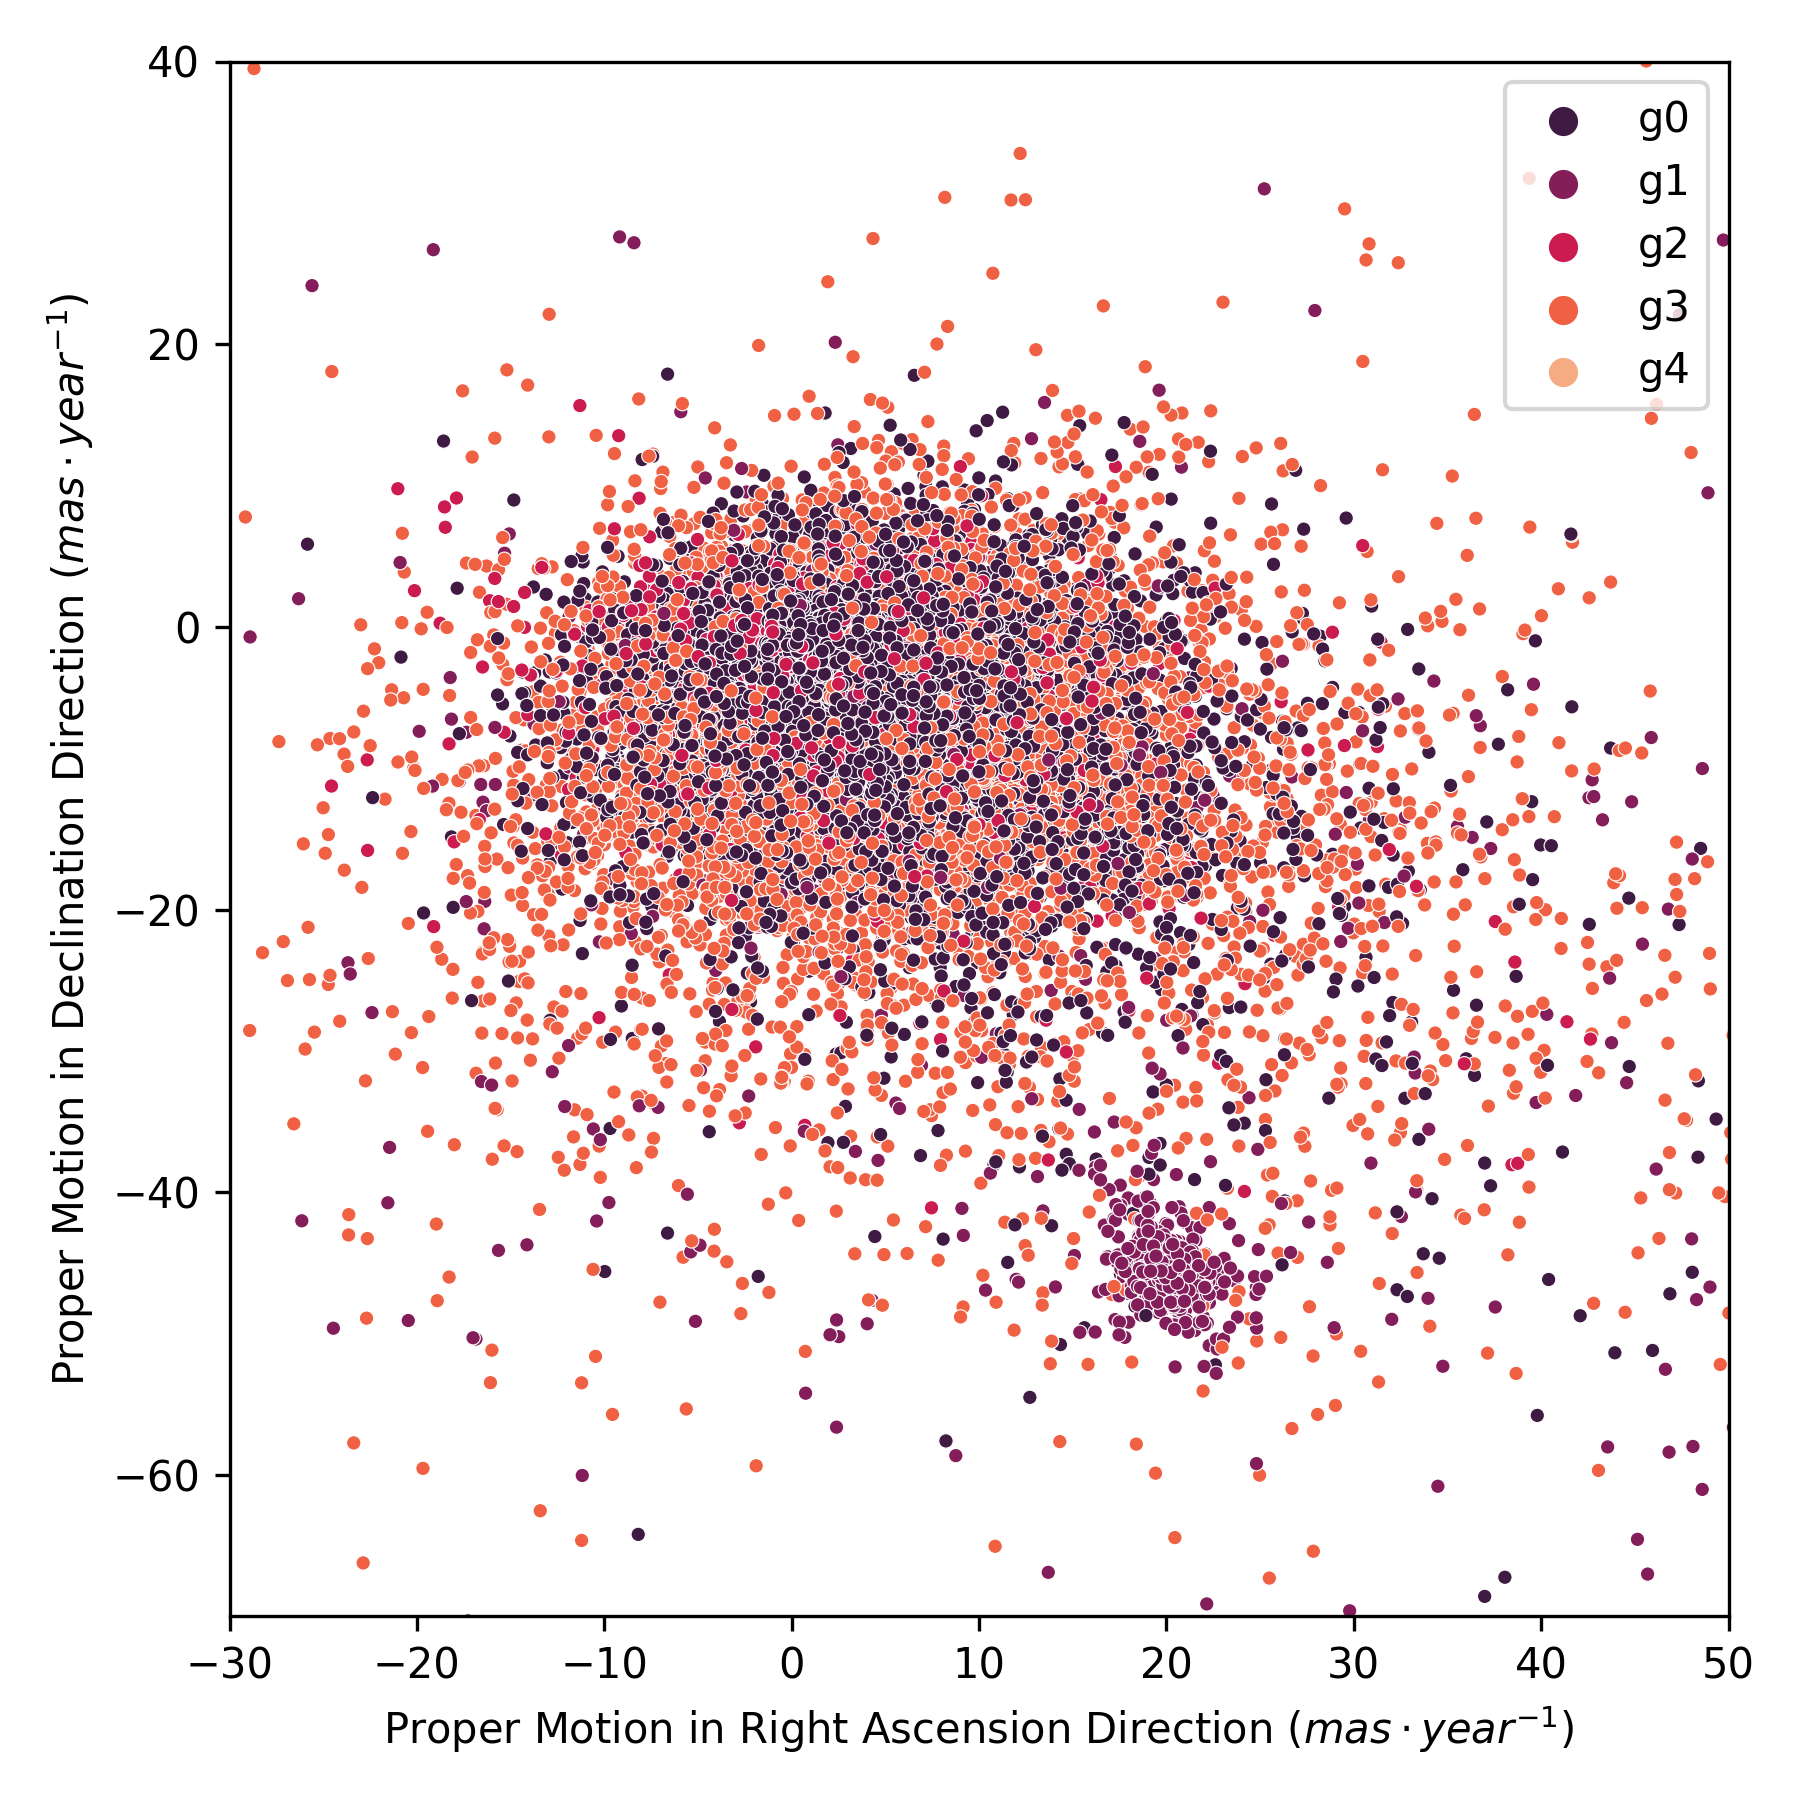
\includegraphics[width=\textwidth]{../figures/melotte_22/kmeans_pm_melotte_22.png}
      \caption{Proper Motion}
    \end{subfigure}
    \hfill
    \begin{subfigure}[t]{.45\textwidth}
      \centering
      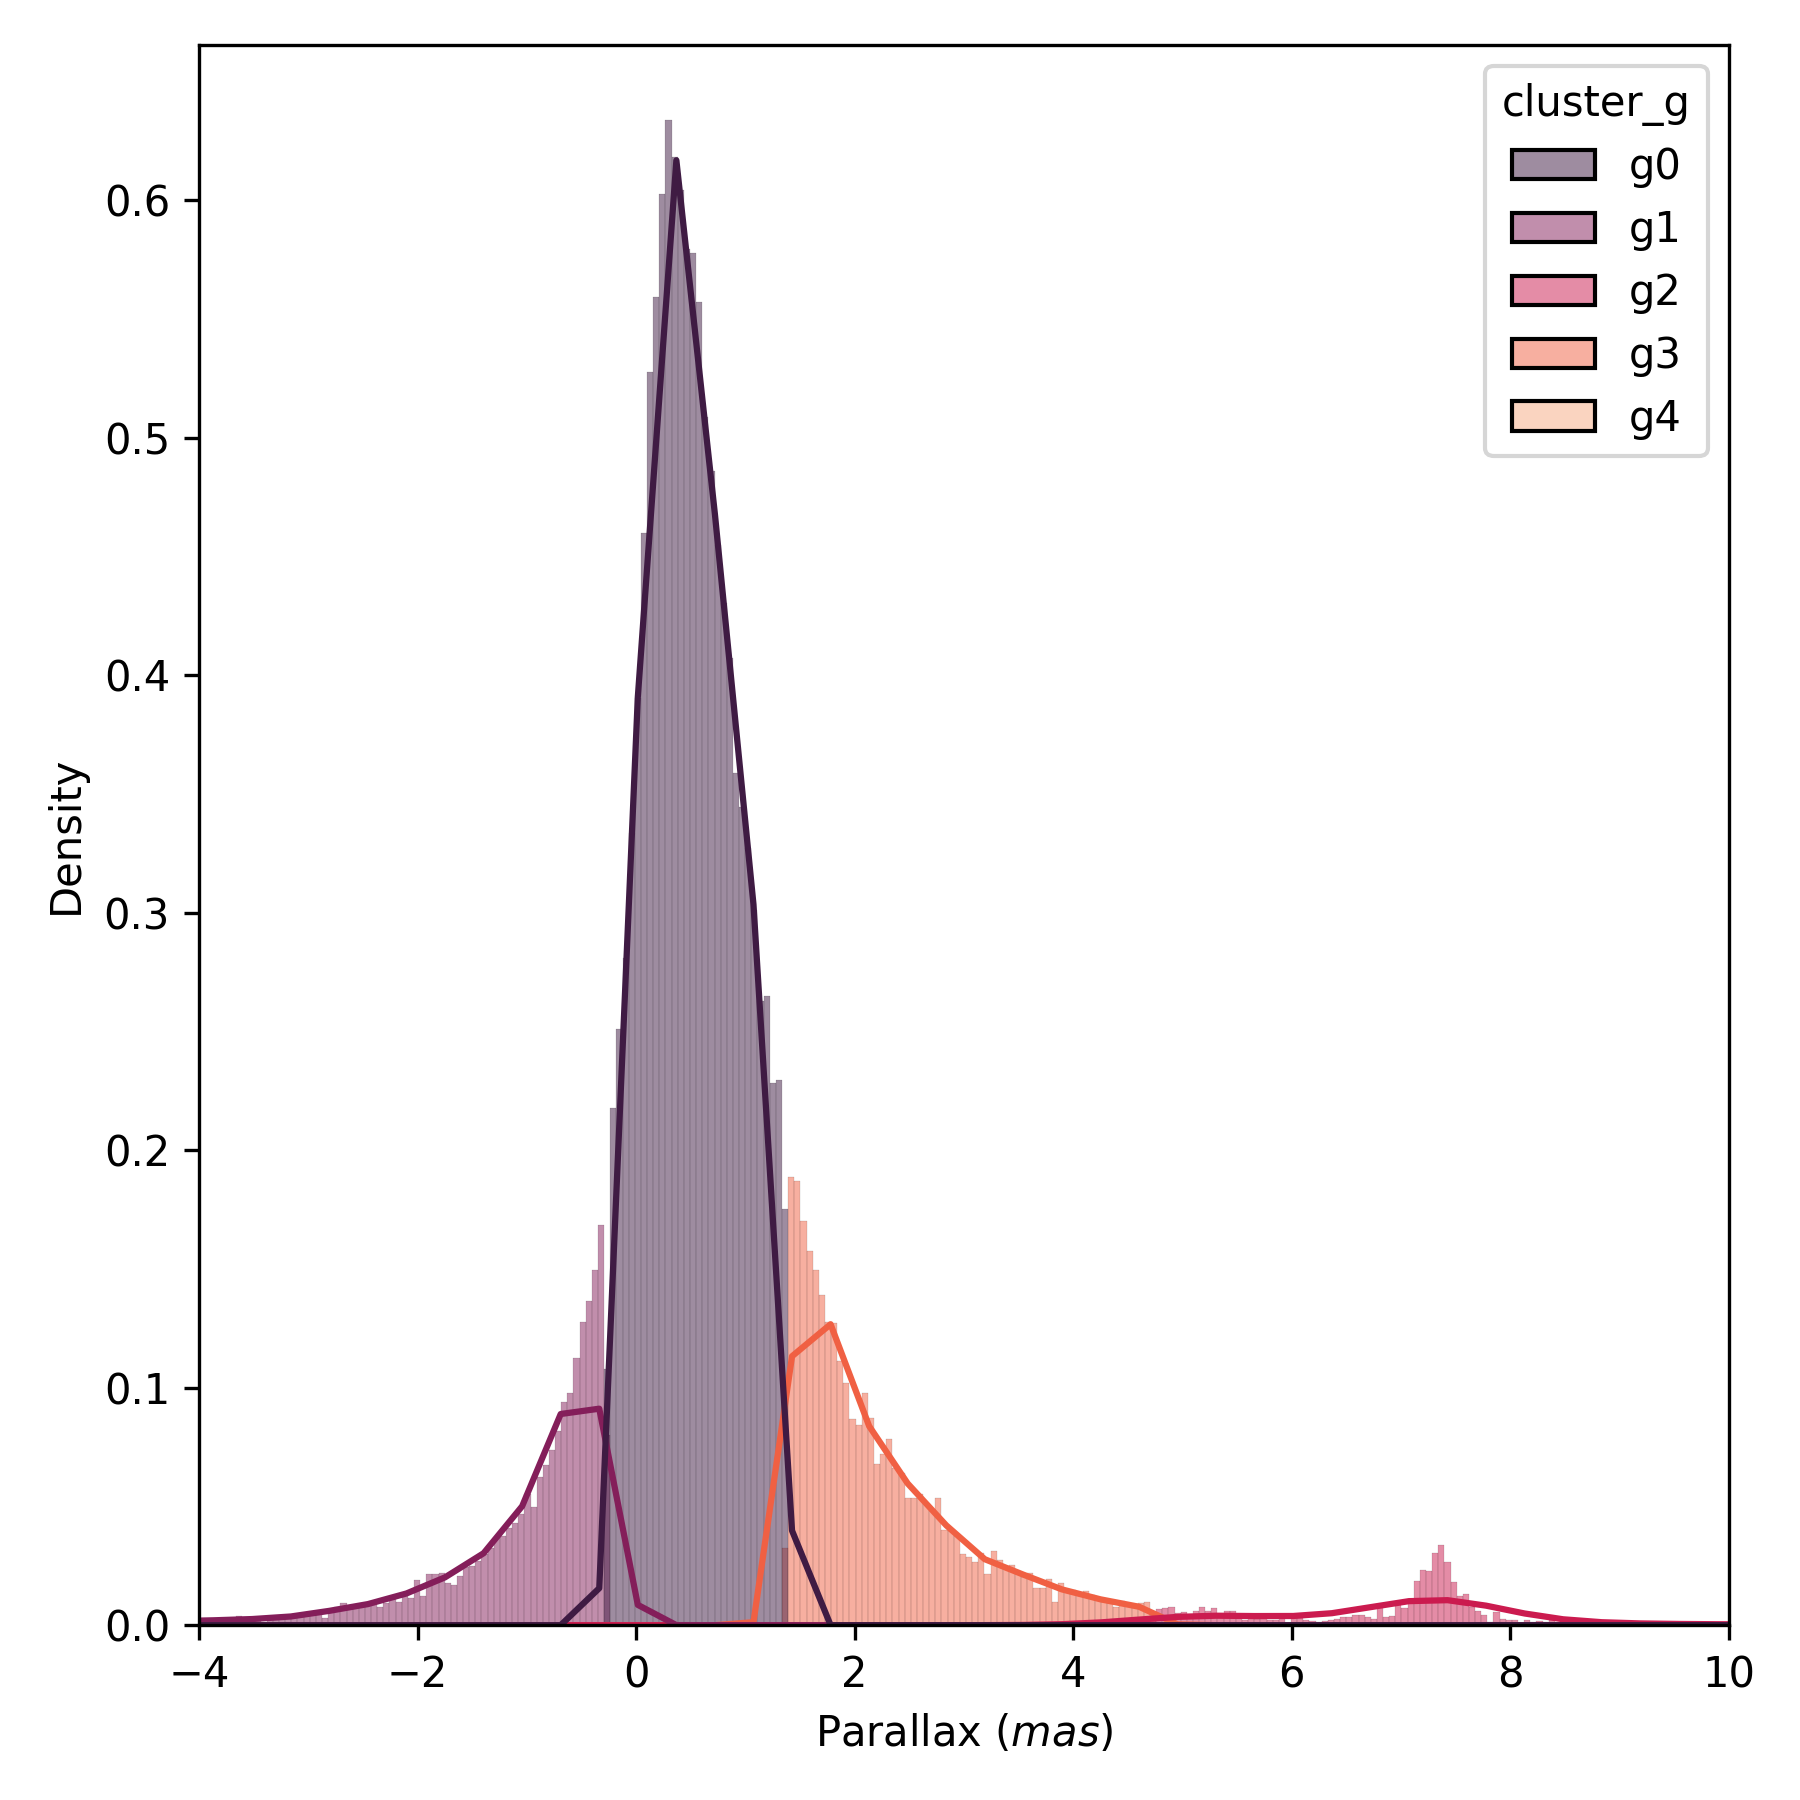
\includegraphics[width=\textwidth]{../figures/melotte_22/kmeans_parallax_melotte_22.png}
      \caption{Parallax}
    \end{subfigure}
  \end{subfigure}
  \caption{K-Means model applied to Melotte 22}
  \label{fig:kmeans_melotte_22}
\end{figure}

If we take a look into the H-R diagram (Figure~\ref{fig:kmeans_hr_diagram_melotte_22}),
we can identify the isochrone curve for Melotte 22 cluster.
This curve has a good shape, but again, it contains outsider stars.
Therefore, we would like to find a better model that improves this initial characterization
by reducing the amount of clusters and also that removes outsiders from the OC.

\begin{figure}[htbp]
  \centering
  \begin{subfigure}{0.5\textwidth}
    \centering
    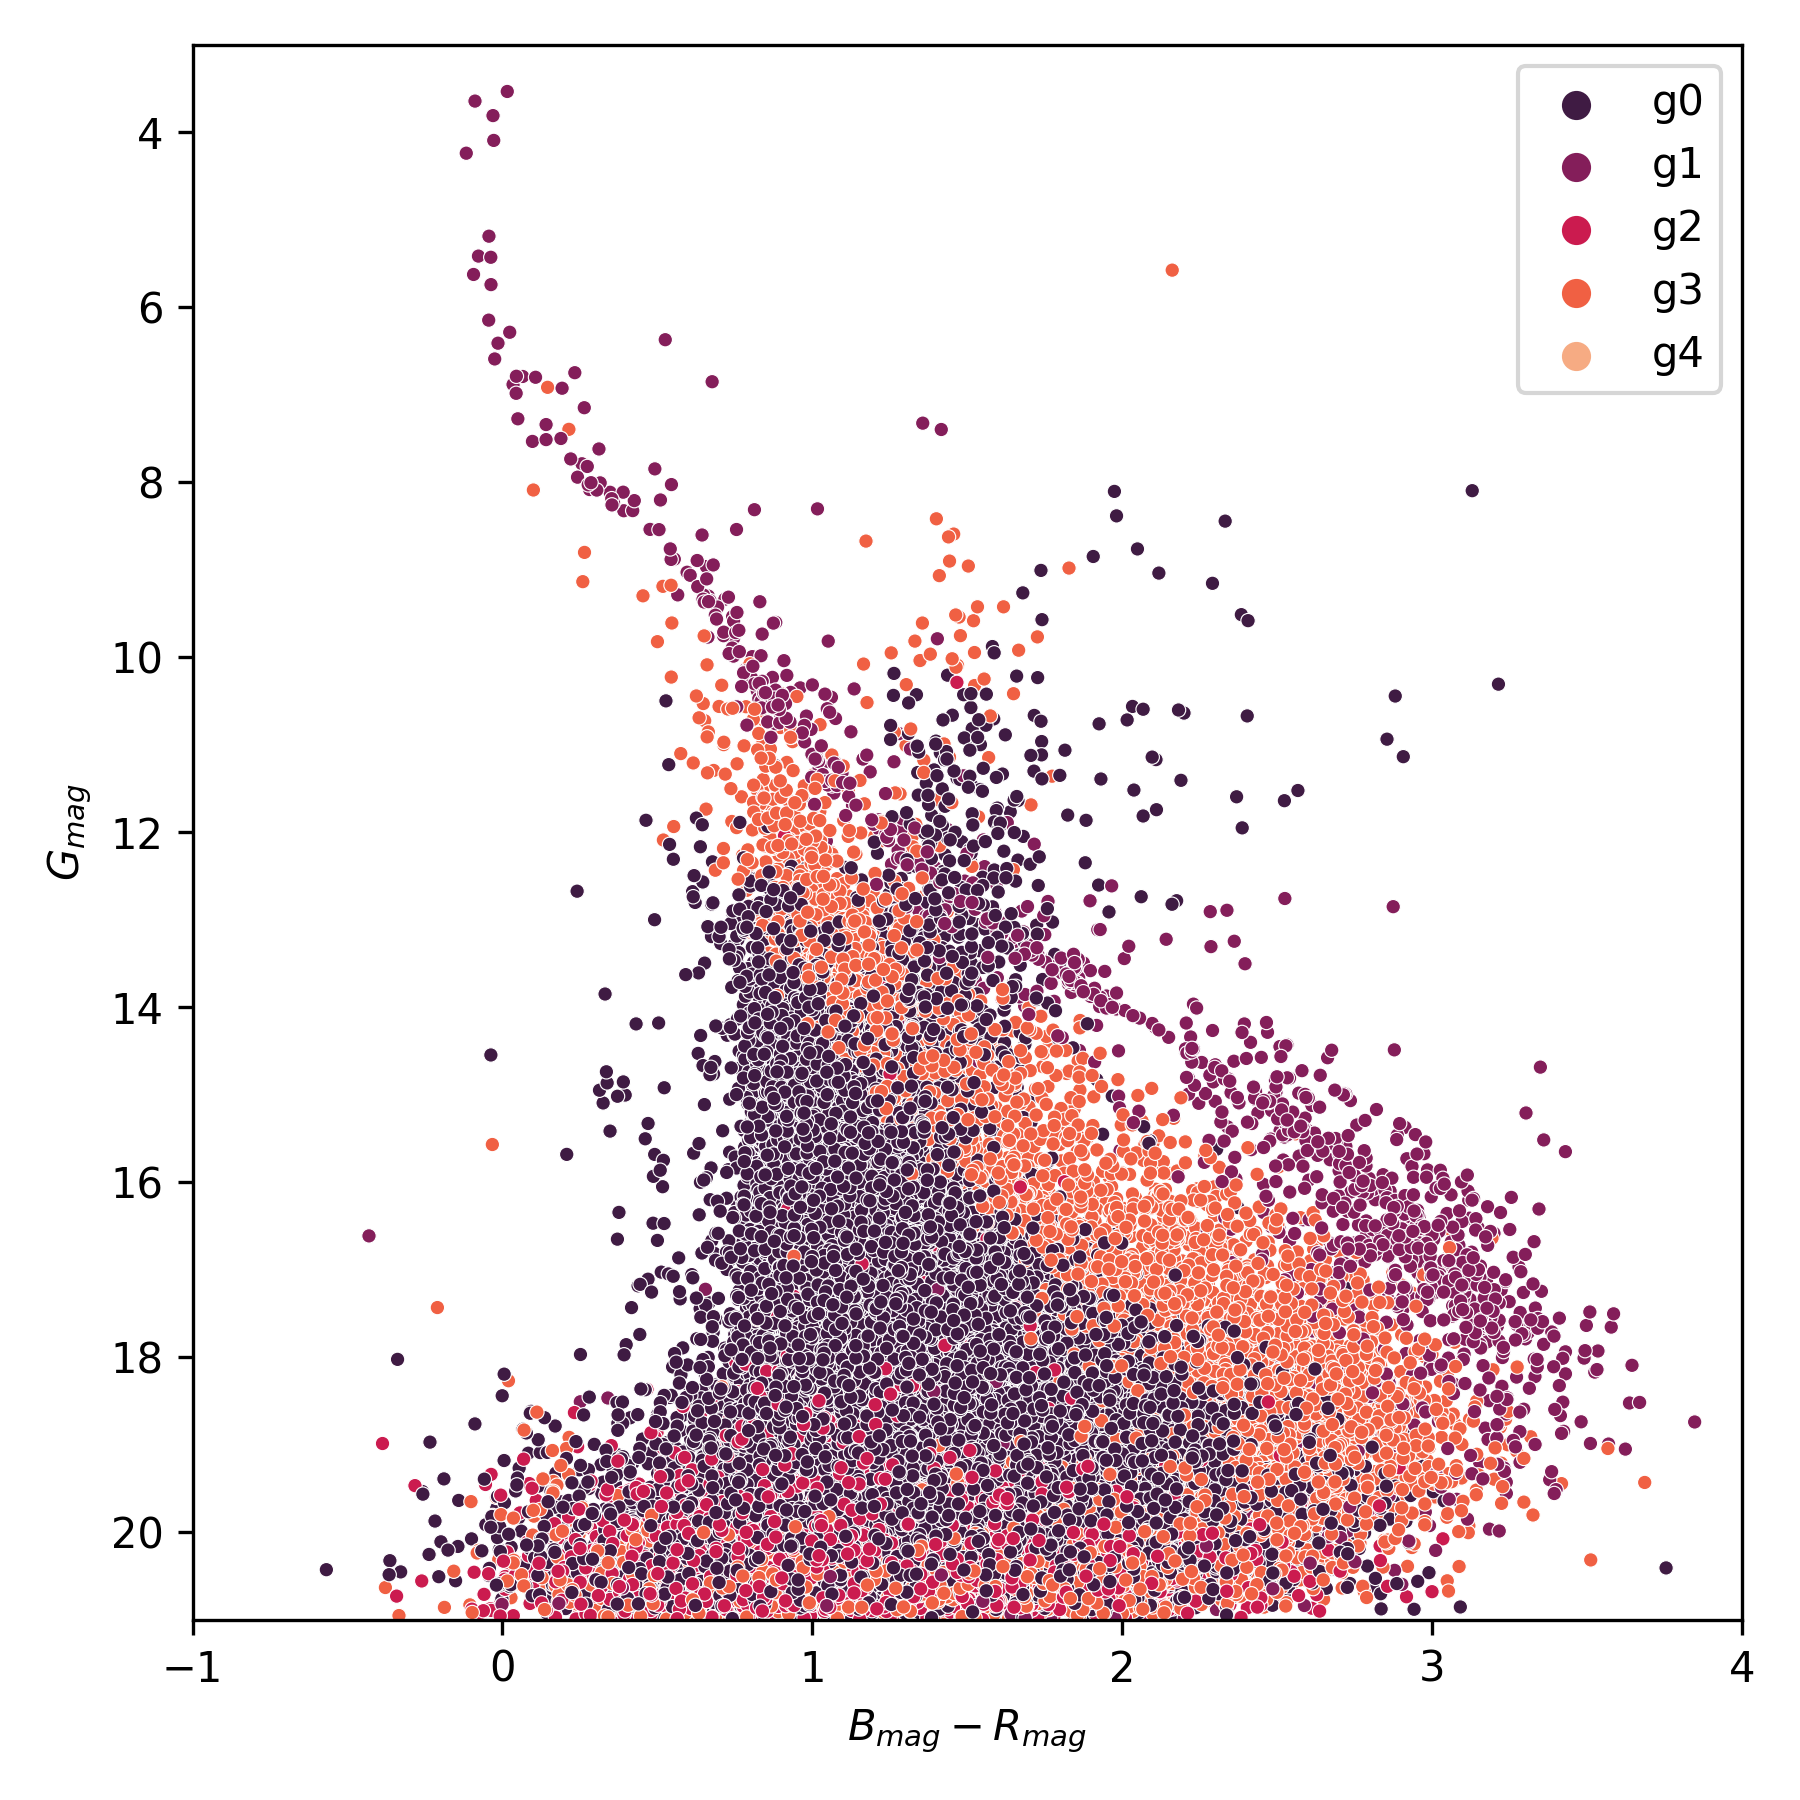
\includegraphics[width=\textwidth]{../figures/melotte_22/kmeans_hr_diagram_melotte_22.png}
  \end{subfigure}
  \caption{Melotte 22 H-R diagram with K-Means characterization}
  \label{fig:kmeans_hr_diagram_melotte_22}
\end{figure}

\section{Deep Embedded Clustering (DEC)}
\label{sec:deep_embedding_clustering}

Our initial approach allows us to find some groups that potentially contain the desired OC.
However, as we have seen before, the result is not accurate enough.
Therefore, we need a method for merging clusters by migrating stars from one group to another,
so we can end up with the minimum number of clusters while preserving the open cluster.

Since we do not have a labeled dataset to train a supervised model,
we have no choice but to use an unsupervised self-trained model.

For that reason we have adapted the \emph{Unsupervised Deep Embedding for Clustering Analysis} to our work.

The implementation of this model is available in \verb|cdalvaro.ml.DEC|
and it is developed with the Keras framework.

The model is composed by a \emph{deep autoencoder} and a \emph{clustering layer}.

The autoencoder is used to transform the input data into a latent space
using a non-linear mapping function \(f_{\theta} : X \rightarrow Z\).

Although, as explained in Section~\ref{sec:feature_selection},
the number of features we are managing is not too large,
this latent space helps us reduce the number of features
and avoids the \emph{``curse of dimensionality``}~\cite{bellman1961curse}.

The autoencoder is pretrained before fitting the model to generate predictions. Then,
the encoder layers of the autoencoder are used with the aim of transforming input data to
the latent space \(Z\). Once the data has been transformed, a K-Means clusterer is used in
order to make an initial clustering. K-Means cluster centers are used as the initial
weights for the clustering layer.

With that initial configuration,
the model iterates alternating between computing an auxiliary target distribution (Soft Assignment)
and minimizing the Kullback-Leiber (KL) divergence~\cite{kullback1951information} to it.
This unsupervised algorithm allows us to improve the clustering.

\begin{equation}
  p_{ij} = \frac{q^{2}_{ij} / f_{j}}{\sum_{j'}q^{2}_{ij'}/f_{j'}}
  \label{eq:student_tdistribution}
\end{equation}

In the soft assignment stage,
the \emph{Student's t-distribution} is used as a kernel to measure the similarity
between the embedded points and the cluster centroid.
While in the KL divergence minimization the algorithm iteratively refines clusters by learning
from their high confidence assignments with the help of an auxiliary target distribution.
The model is trained by matching the soft assignment to the target distribution.
The choice of this target distribution is crucial for DEC's performance.
In this work we have taken the target distribution from DEC's original paper~\cite{xie2016unsupervised},
which is defined in Equation~\ref{eq:student_tdistribution}.

Figure~\ref{fig:dec_model_setup} shows the layer setup of our DEC model.
It is simpler than the one tested on the original paper~\cite{xie2016unsupervised},
since the number of selected features in our work is smaller than in the original one.
Therefore, using the same configuration would result in a model so
powerful that would incur in overfitting issues unable to make right predictions.

\begin{figure}[htbp]
  \centering
  \begin{subfigure}{0.9\textwidth}
    \centering
    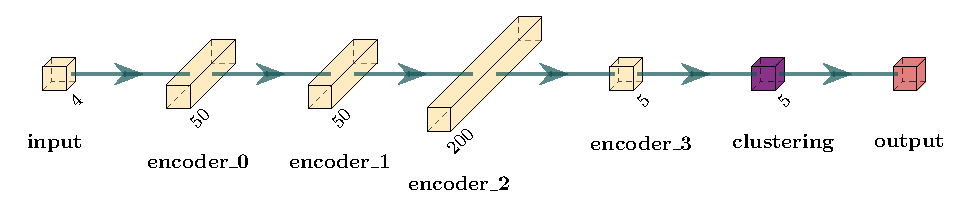
\includegraphics[width=\textwidth]{../figures/dec_diagram.pdf}
  \end{subfigure}
  \caption{DEC model layer setup}
  \label{fig:dec_model_setup}
\end{figure}

Once the model is ready, we can test it by applying it to the Melotte 22 dataset.
Notebook \verb|cluster_characterization.ipynb| illustrates how DEC model processes a region of stars
trying to characterize the open cluster hidden within that region.

As shown in Figure~\ref{fig:dec_melotte_22},
the DEC model is able to move stars from one group to another,
removing some clusters and improving the OC characterization.
This is exactly what we are looking for.

\begin{figure}[htbp]
  \centering
  \begin{subfigure}{0.9\textwidth}
    \centering
    \begin{subfigure}[t]{0.45\textwidth}
      \centering
      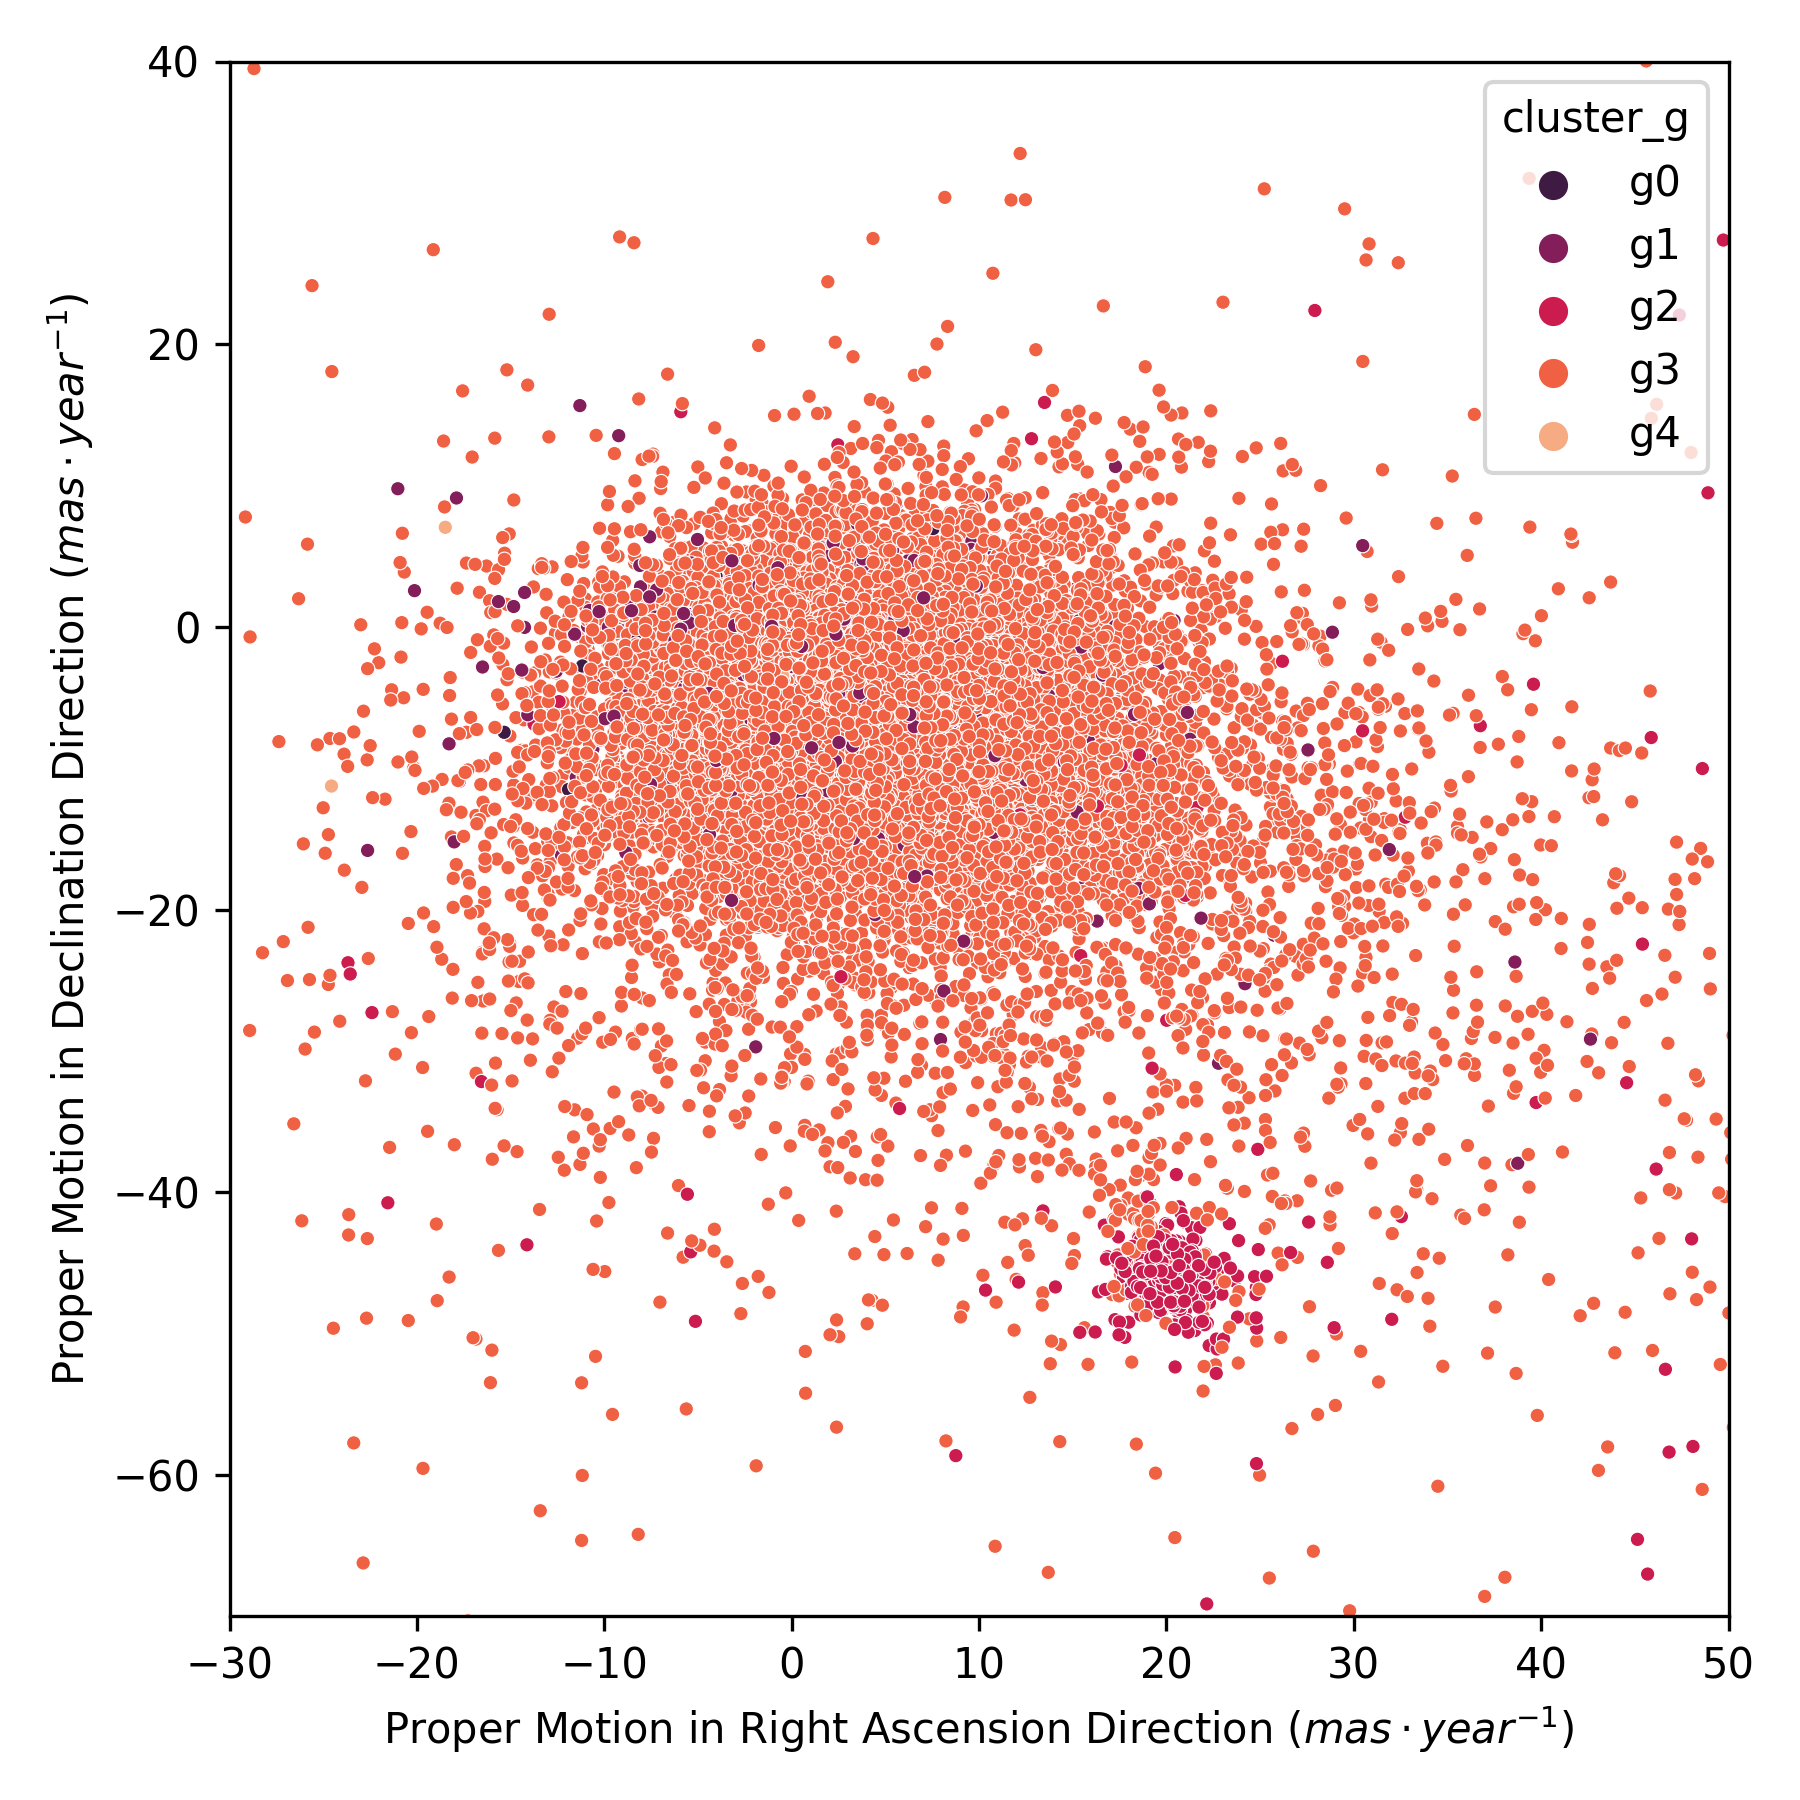
\includegraphics[width=\textwidth]{../figures/melotte_22/dec_pm_melotte_22.png}
      \caption{Proper Motion}
    \end{subfigure}
    \hfill
    \begin{subfigure}[t]{0.45\textwidth}
      \centering
      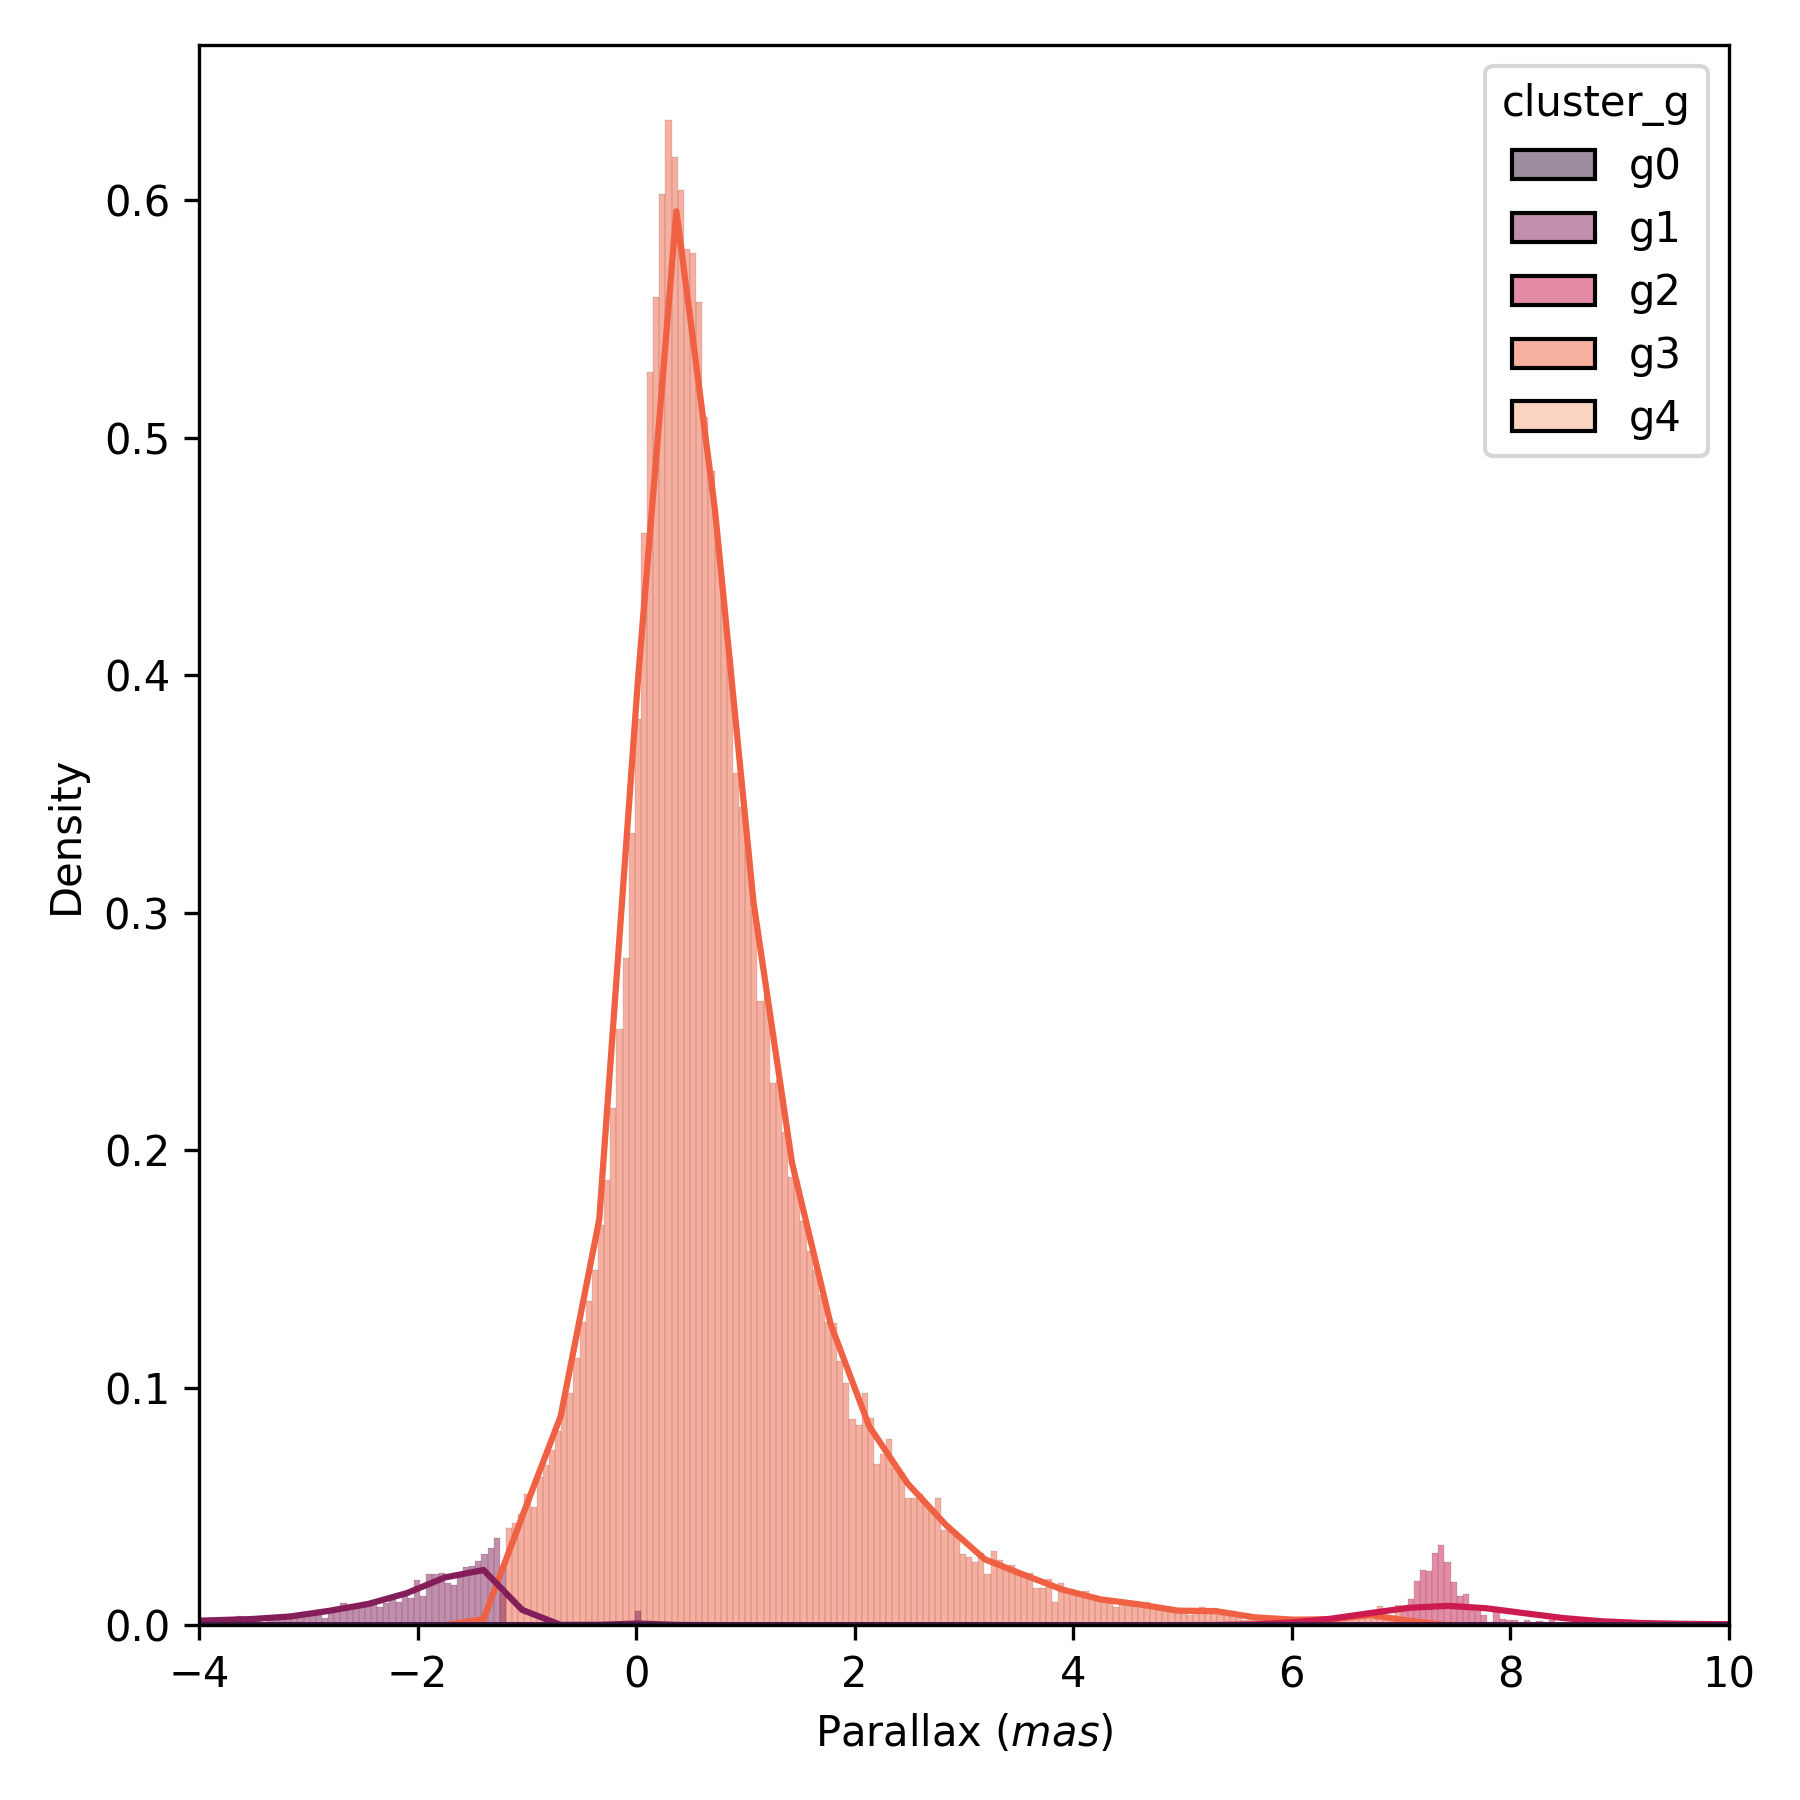
\includegraphics[width=\textwidth]{../figures/melotte_22/dec_parallax_melotte_22.png}
      \caption{Parallax}
    \end{subfigure}
  \end{subfigure}
  \caption{DEC model applied to Melotte 22}
  \label{fig:dec_melotte_22}
\end{figure}

The H-R diagram has been improved as well,
and the isochrone curve of the open cluster is sharper than the one obtained with the K-Means algorithm
(Figure~\ref{fig:kmeans_hr_diagram_melotte_22}).

Figure~\ref{fig:hr_diagram_comparison} shows a comparison between the H-R diagram obtained
by DEC clustering and the one obtained using the Clusterix + TOPCAT method.

\begin{figure}[htbp]
  \centering
  \begin{subfigure}{0.9\textwidth}
    \centering
    \begin{subfigure}[t]{0.45\textwidth}
      \centering
      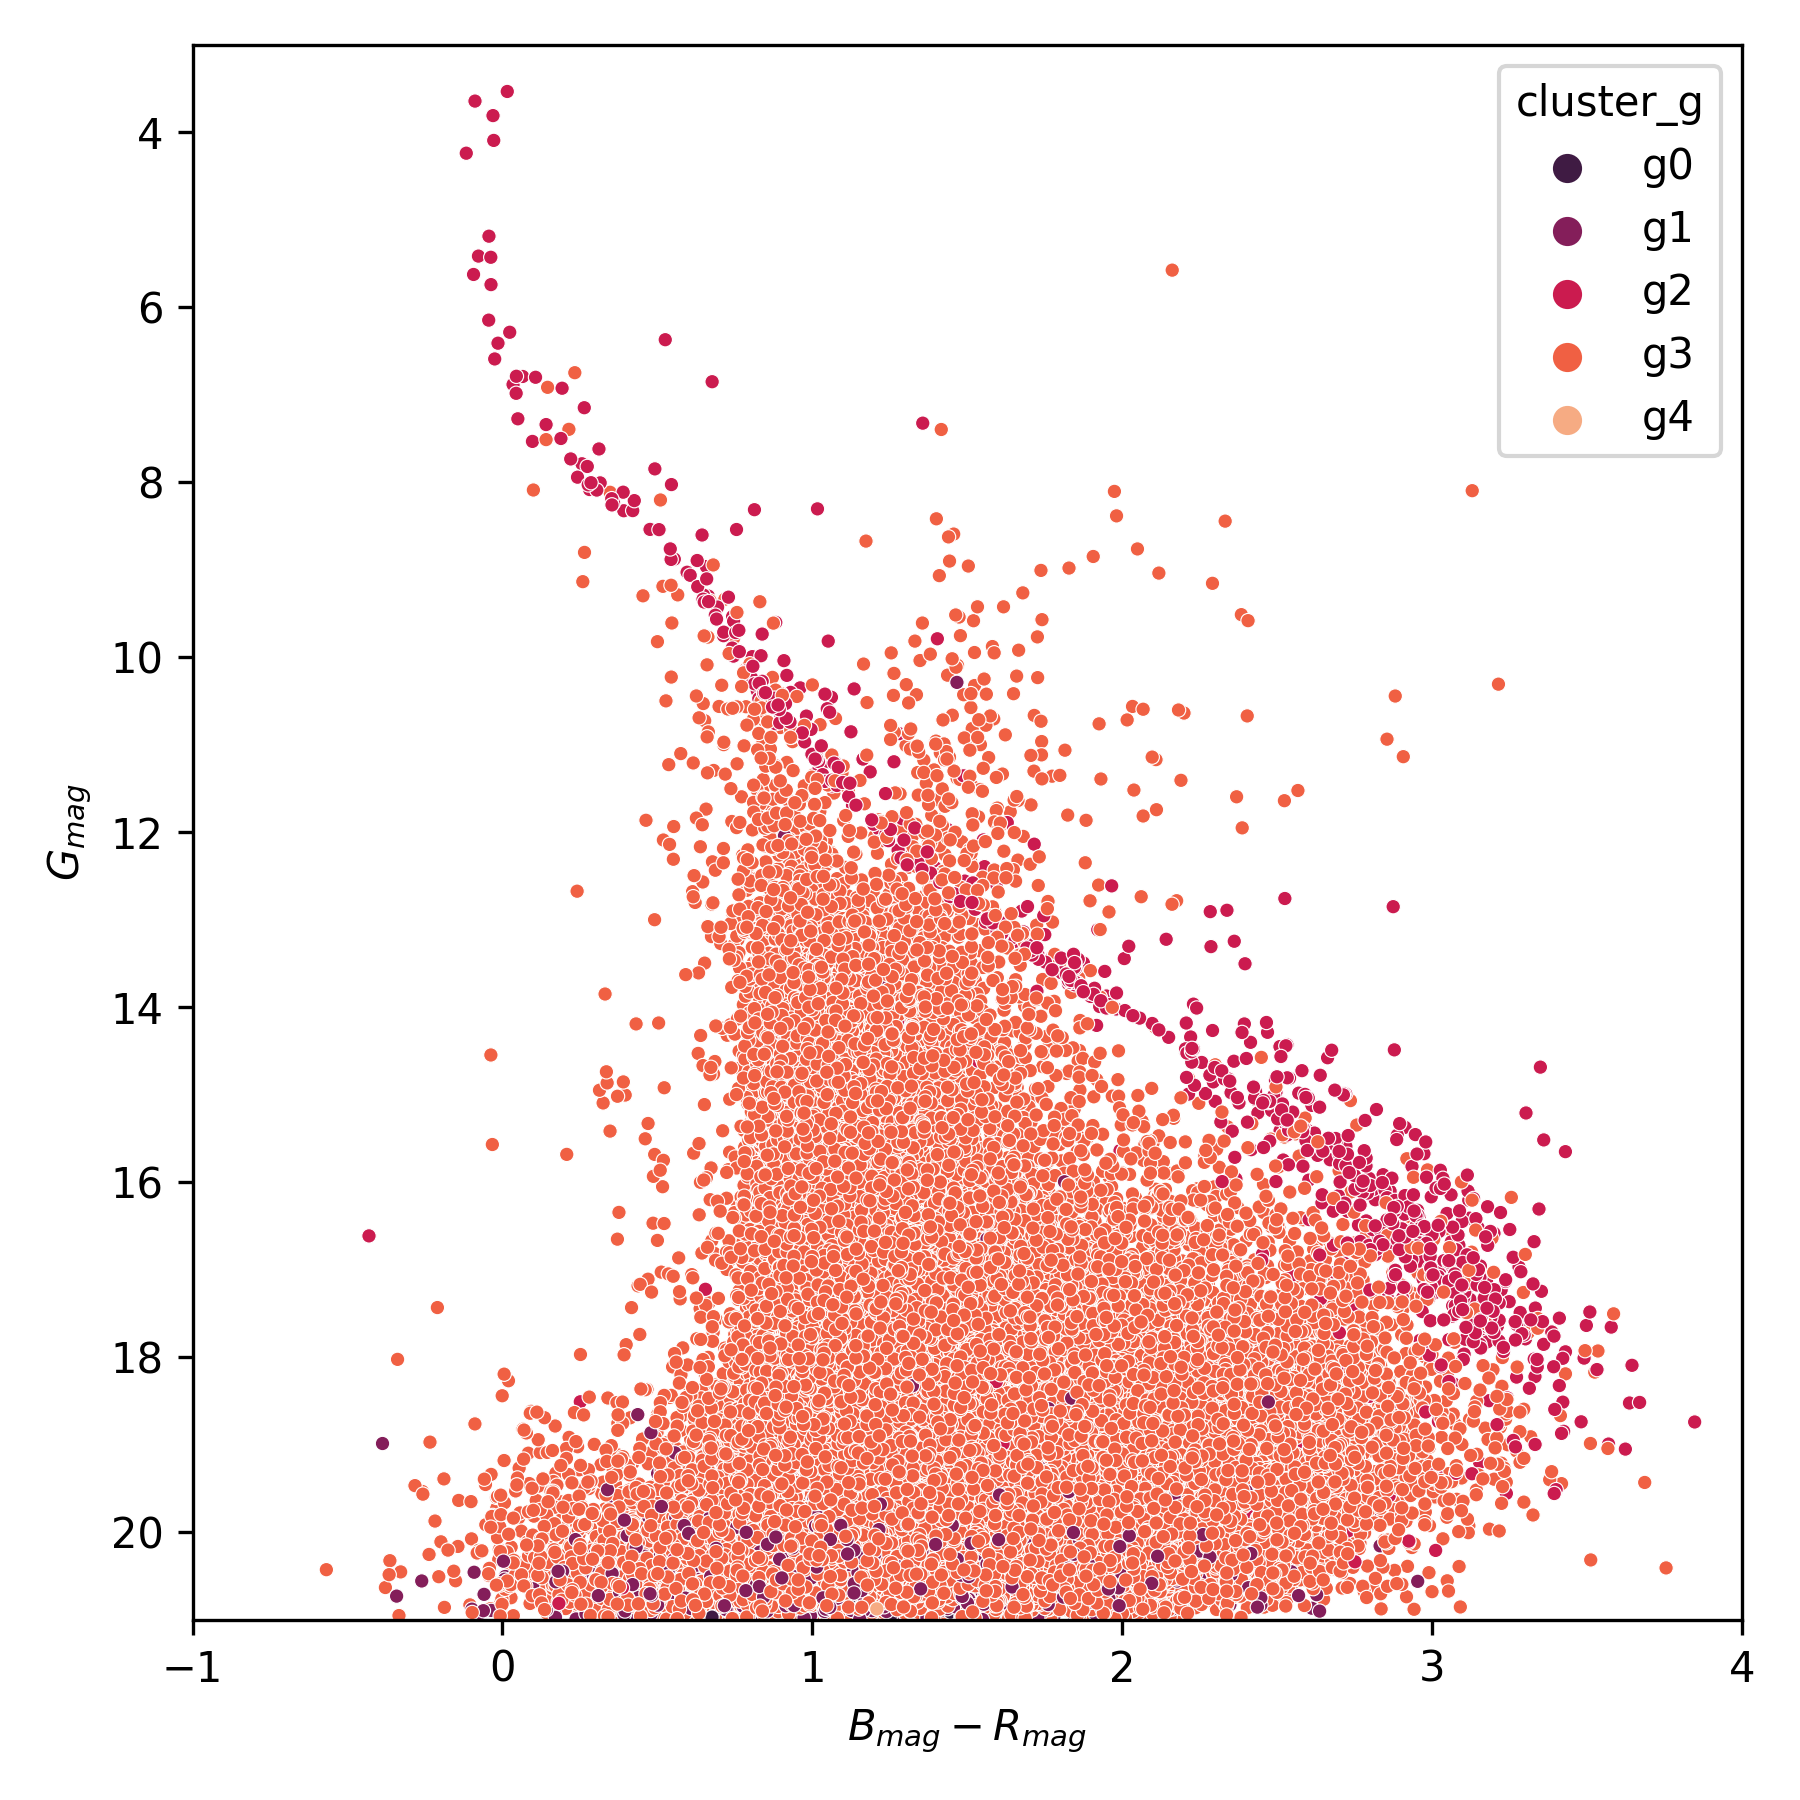
\includegraphics[width=\textwidth]{../figures/melotte_22/dec_hr_diagram_melotte_22.png}
      \caption{DEC H-R diagram}
    \end{subfigure}
    \hfill
    \begin{subfigure}[t]{0.45\textwidth}
      \centering
      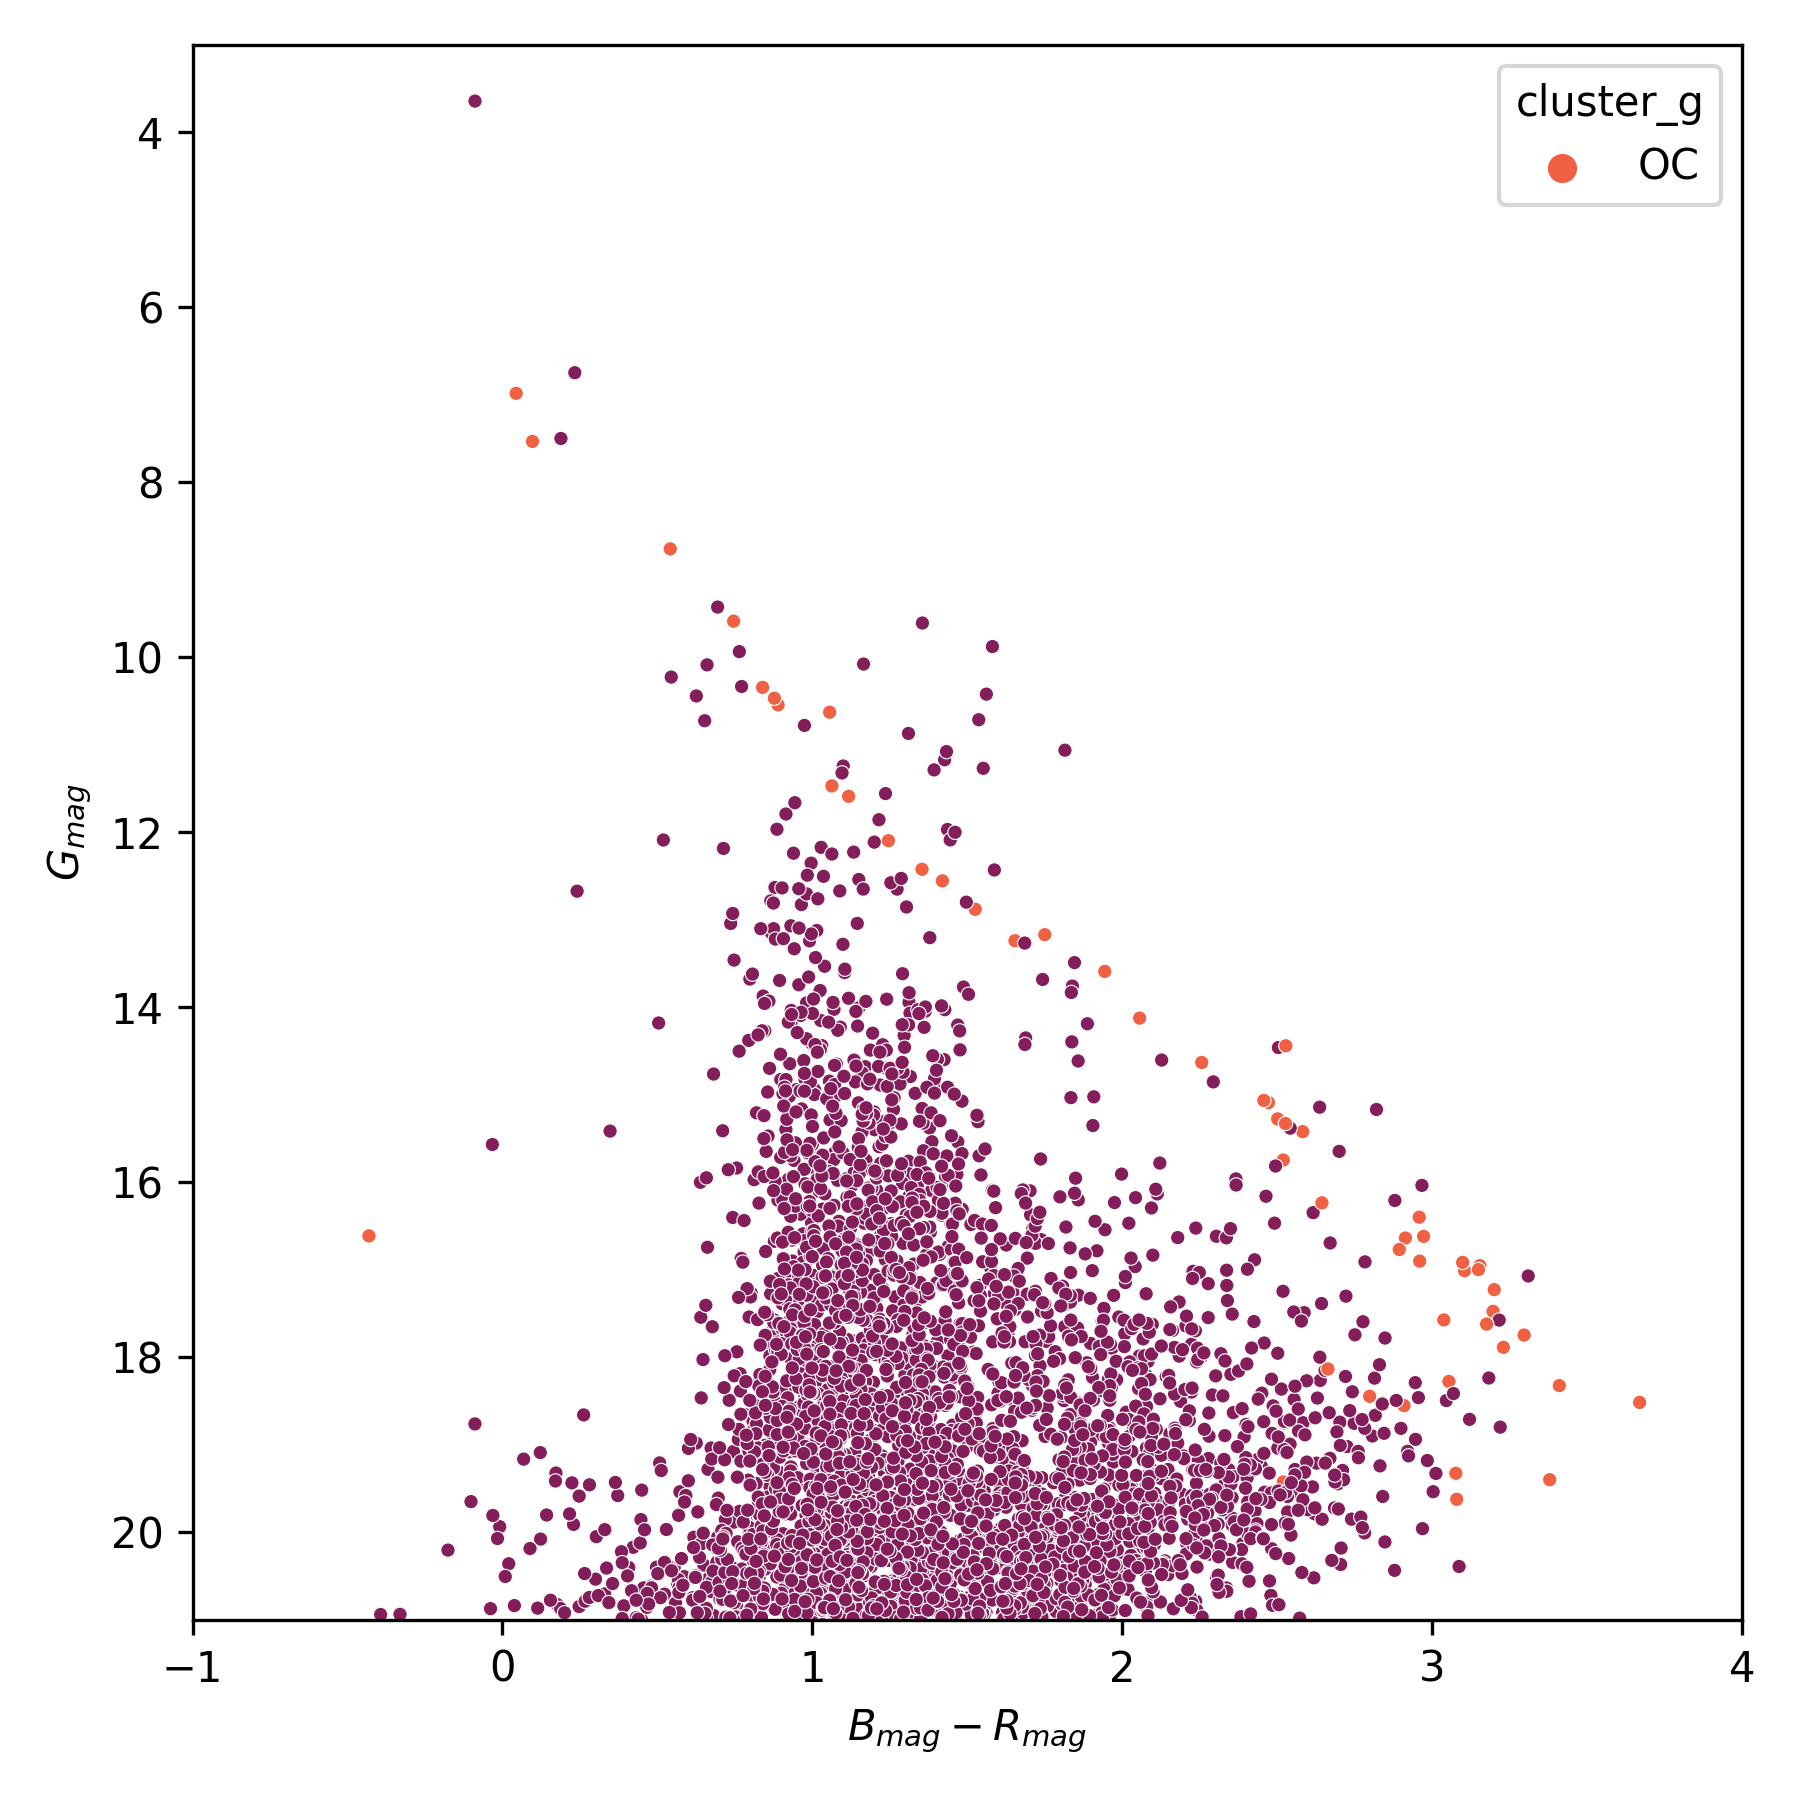
\includegraphics[width=\textwidth]{../figures/melotte_22/hr_diagram_melotte_22.png}
      \caption{Clusterix+TOPCAT H-R diagram}
    \end{subfigure}
  \end{subfigure}
  \caption{H-R diagram comparison between DEC clustering and Clusterix+TOPCAT method.}
  \label{fig:hr_diagram_comparison}
\end{figure}

Finally, we can refine this selection by filtering those stars which are bellow and above
the 0.10 and 0.90 quantiles for each group, respectively.
That way we remove the most doubtful values from the selection.
Figure~\ref{fig:melotte_22_filtered} shows the result after filtering DEC clustering selection.

\begin{figure}[htbp]
  \centering
  \begin{subfigure}{0.9\textwidth}
    \centering
    \begin{subfigure}[t]{0.45\textwidth}
      \centering
      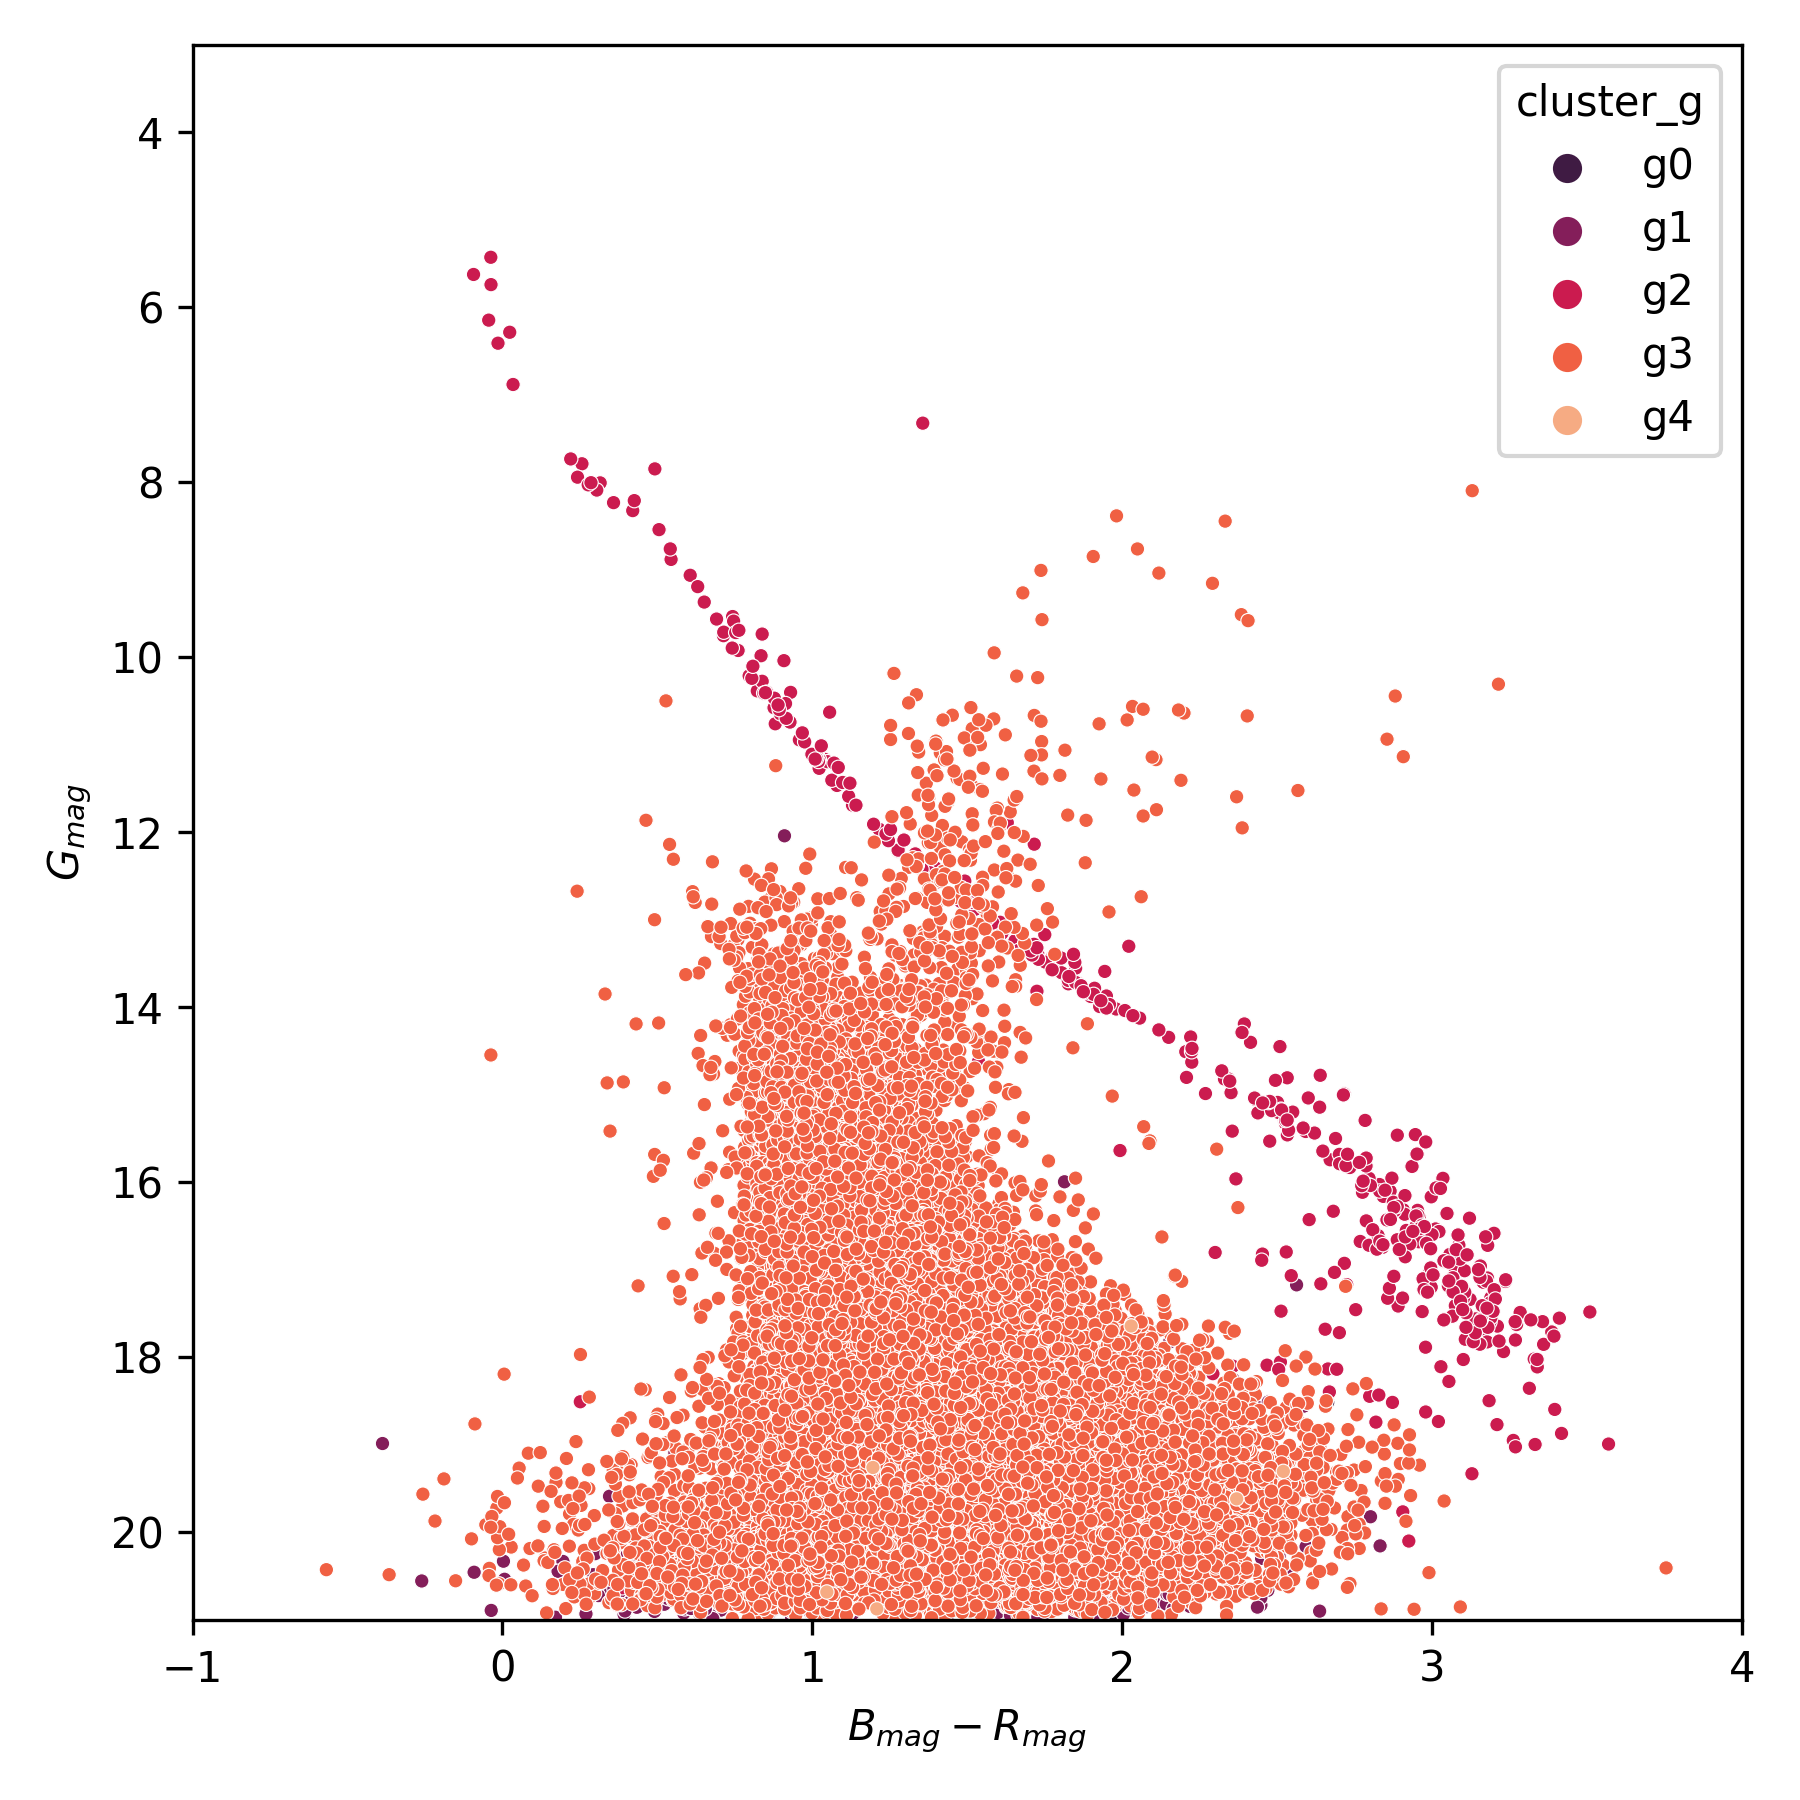
\includegraphics[width=\textwidth]{../figures/melotte_22/dec_hr_diagram_filtered_melotte_22.png}
      \caption{H-R diagram}
    \end{subfigure}
    \hfill
    \begin{subfigure}[t]{0.45\textwidth}
      \centering
      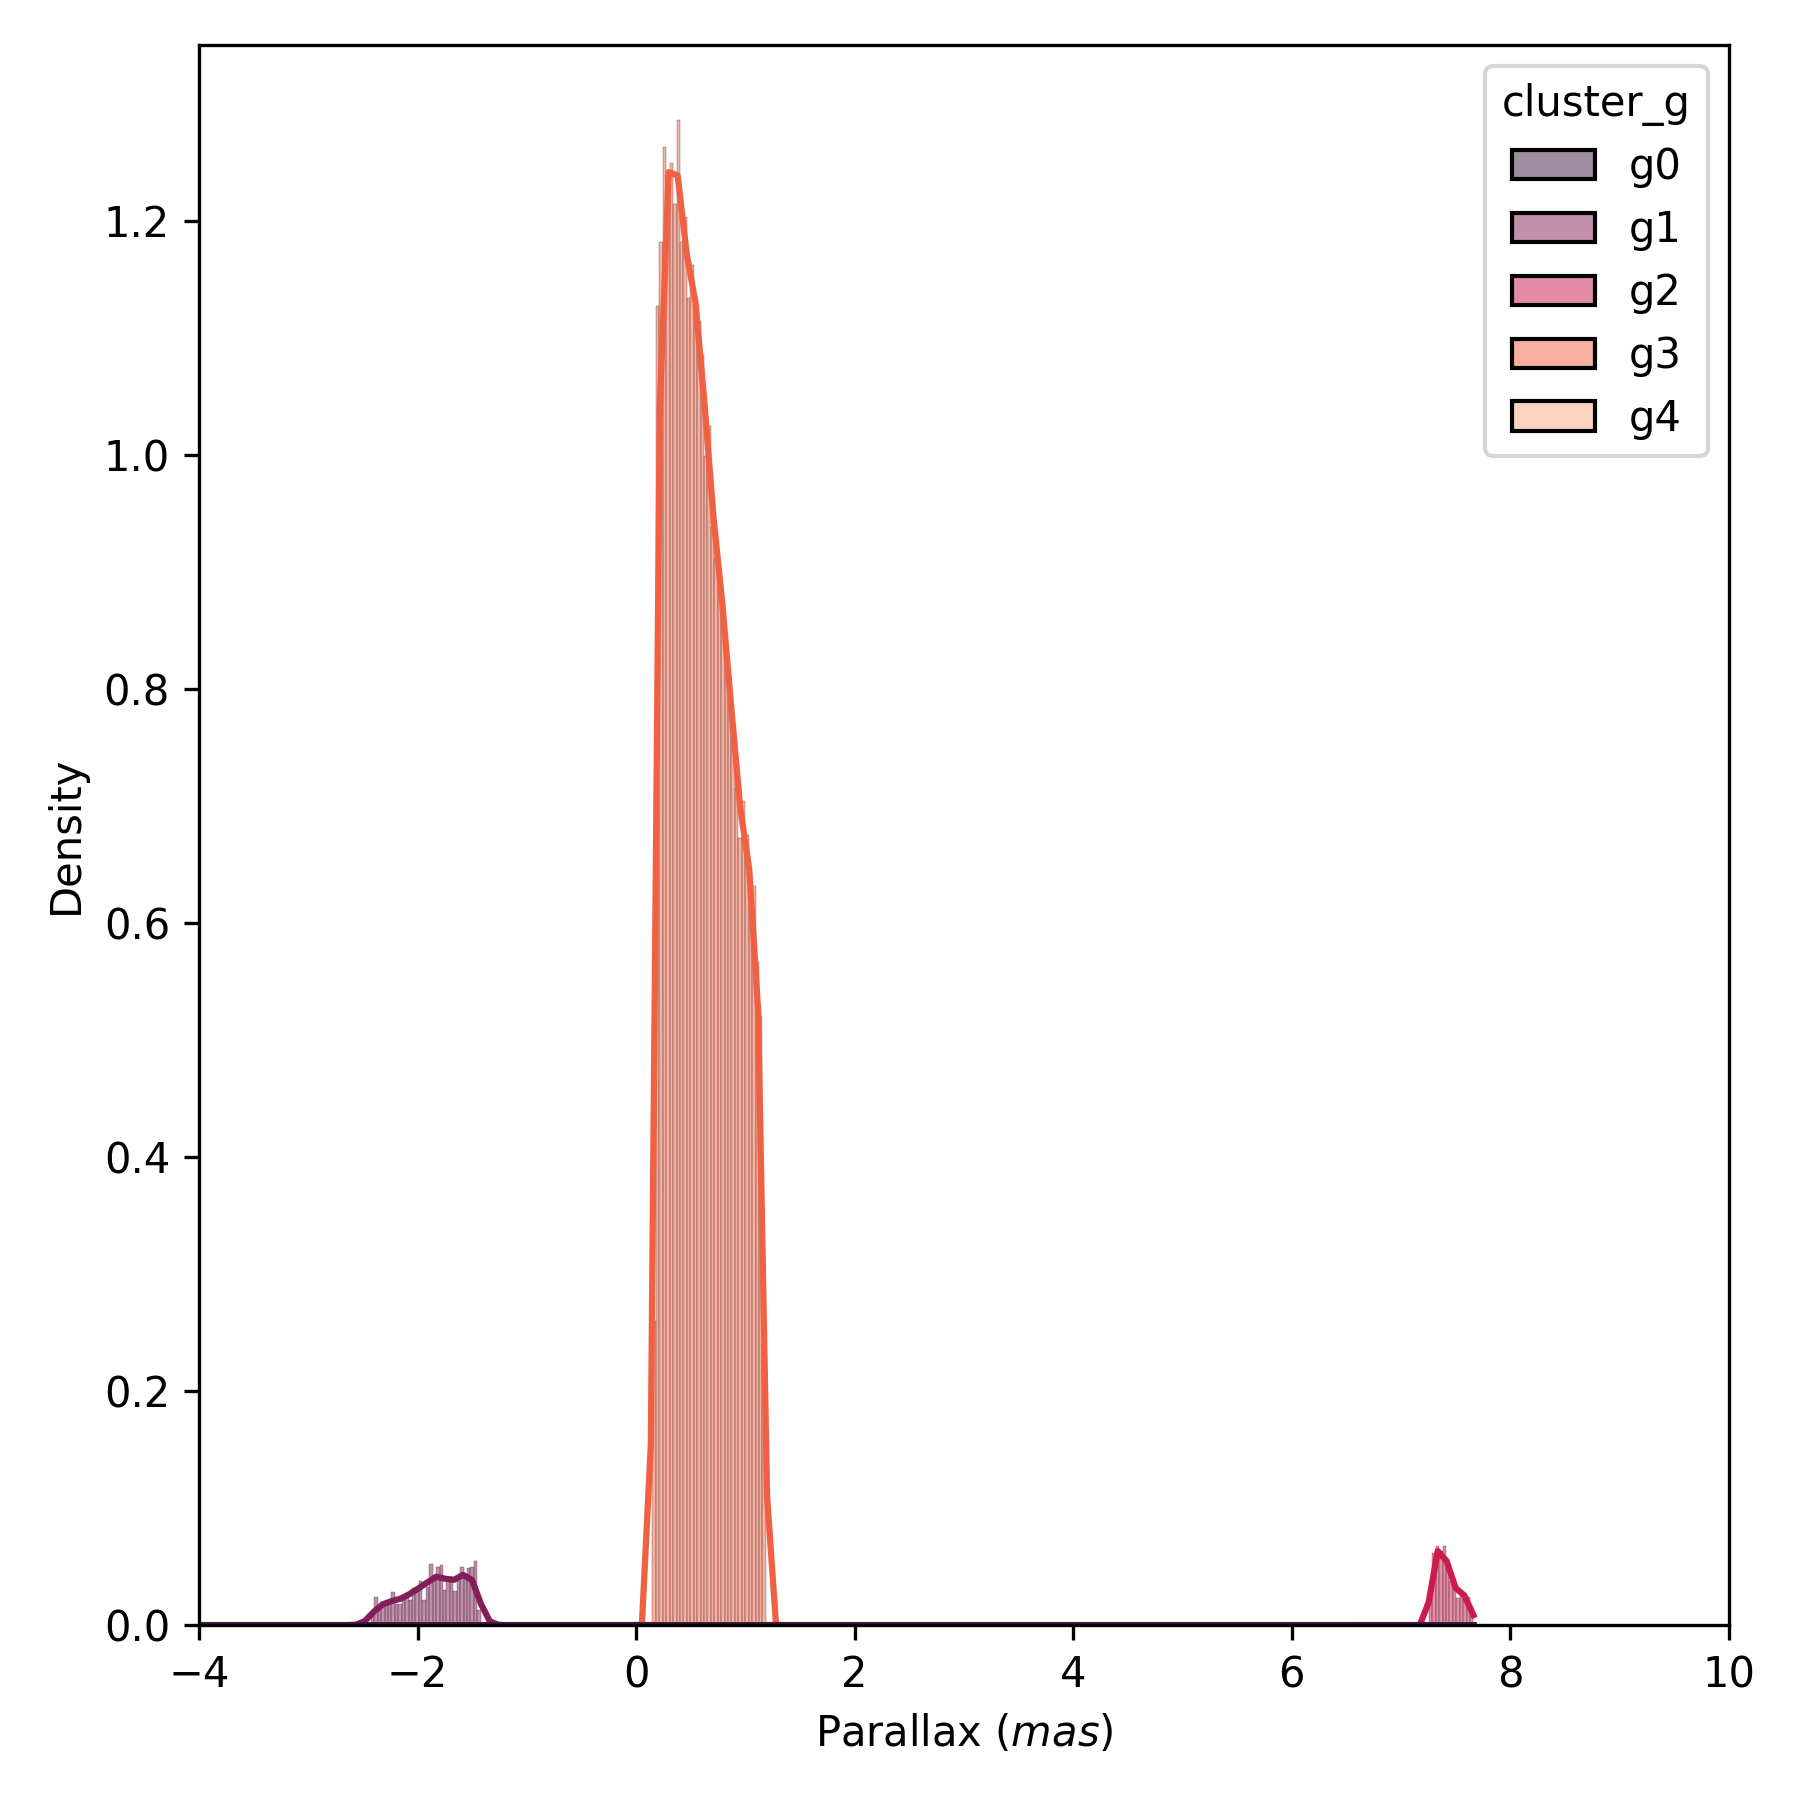
\includegraphics[width=\textwidth]{../figures/melotte_22/dec_parallax_filtered_melotte_22.png}
      \caption{Parallax}
    \end{subfigure}
  \end{subfigure}
  \caption{Melotte 22 H-R diagram and parallax histogram with stars outside 0.25 and 0.75 quantiles filtered.}
  \label{fig:melotte_22_filtered}
\end{figure}

Table~\ref{tab:results_melotte_22} shows a summary of Melotte 22 with values taken from different sources and methods:
SIMBAD Astronomical Database - CDS (Strasbourg),
Clusterix+TOPCAT method, and the results obtained for each step of this method (K-Means, DEC and DEC filtered).
Errors associated to K-Means and DEC predictions have been calculated as the \emph{Standard Error},
\(SE = \sigma / \sqrt{N}\), where \(N\) is the number of samples in the selected group.

\vfill
\begin{table}[h]
  \begin{center}
    \begin{tabular}{l|c|c|c|c}
      \textbf{Source / method} & \emph{\(\mu_{\alpha}\) \((mas \cdot yr^{-1})\)} & \emph{\(\mu_{\delta}\) \((mas \cdot yr^{-1})\)}
      & \emph{\( \varpi \) \((mas)\)} & \emph{\# stars} \\
      \hline
      \textbf{Simbad.u-strasbg.fr}\tablefootnote{Results have been taken from \protect\citeA[p.~25. Table A.3. Pleiades]{babusiaux2018gaia}} &
        19.997 \( \pm \) 0.127 & -45.548 \( \pm \) 0.101 & 7.364 \( \pm \) 0.005 & 1326 \\
      Clusterix+TOPCAT & 19.98 \( \pm \) 1.25 & -45.47 \( \pm \) 1.48 & 7.33 \( \pm \) 0.21 & 634 \\
      K-Means & 20.25 \( \pm \) 0.95 & -38.01 \( \pm \) 1.08 & 7.23 \( \pm \) 0.06 & 1378 \\
      DEC & 23.67 \( \pm \) 1.29 & -46.23 \( \pm \) 1.50 & 8.04 \( \pm \) 0.09 & 878 \\
      \textbf{DEC (filtered)} & 19.50 \( \pm \) 0.41 & -44.23 \( \pm \) 0.39 & 7.42 \( \pm \) 0.005 & 438 \\
    \end{tabular}
    \caption{Parameters shown are proper motion in right ascension and declination, parallax
             with their respective deviations and number of stars corresponding to Melotte 22 data.}
    \label{tab:results_melotte_22}
  \end{center}
\end{table}
\vfill

\chapter{Results}

We have seen in Section~\ref{sec:deep_embedding_clustering} that DEC model is capable
of refining the clustering selection made by K-Means
hence helping us have a more precise characterization of the cluster.
Now, in order to validate our model and to be able to estimate how good or bad it is,
we need a different technique to characterize the studied clusters and compare our results
with those obtained with the validation method.

For that purpose, we have used an alternative method based on Virtual Observatory (VO) tools
such as Clusterix and TOPCAT, to characterize the studied clusters.

\section{Cluster Characterization with VO Tools}

The aim of this section is to highlight the procedure differences between our method and the validation one,
as well as using the results provided by the second technique to validate ours results.
This validation method uses a combination of VO tools: \emph{Clusterix 2.0 + TOPCAT}.
We take Melotte 22 again as our study case to make easier the comparison process between
the method presented in Chapter~\ref{chap:method} and the alternative one.

The initial point is taking advantage of Clusterix in order to avoid a subjective
and manual selection for the cluster members.
Figure~\ref{fig:clusterix_selection} shows a screenshot of the Clusterix 2.0 selection panel.

\begin{figure}[htbp]
  \centering
  \begin{subfigure}{0.9\textwidth}
    \centering
    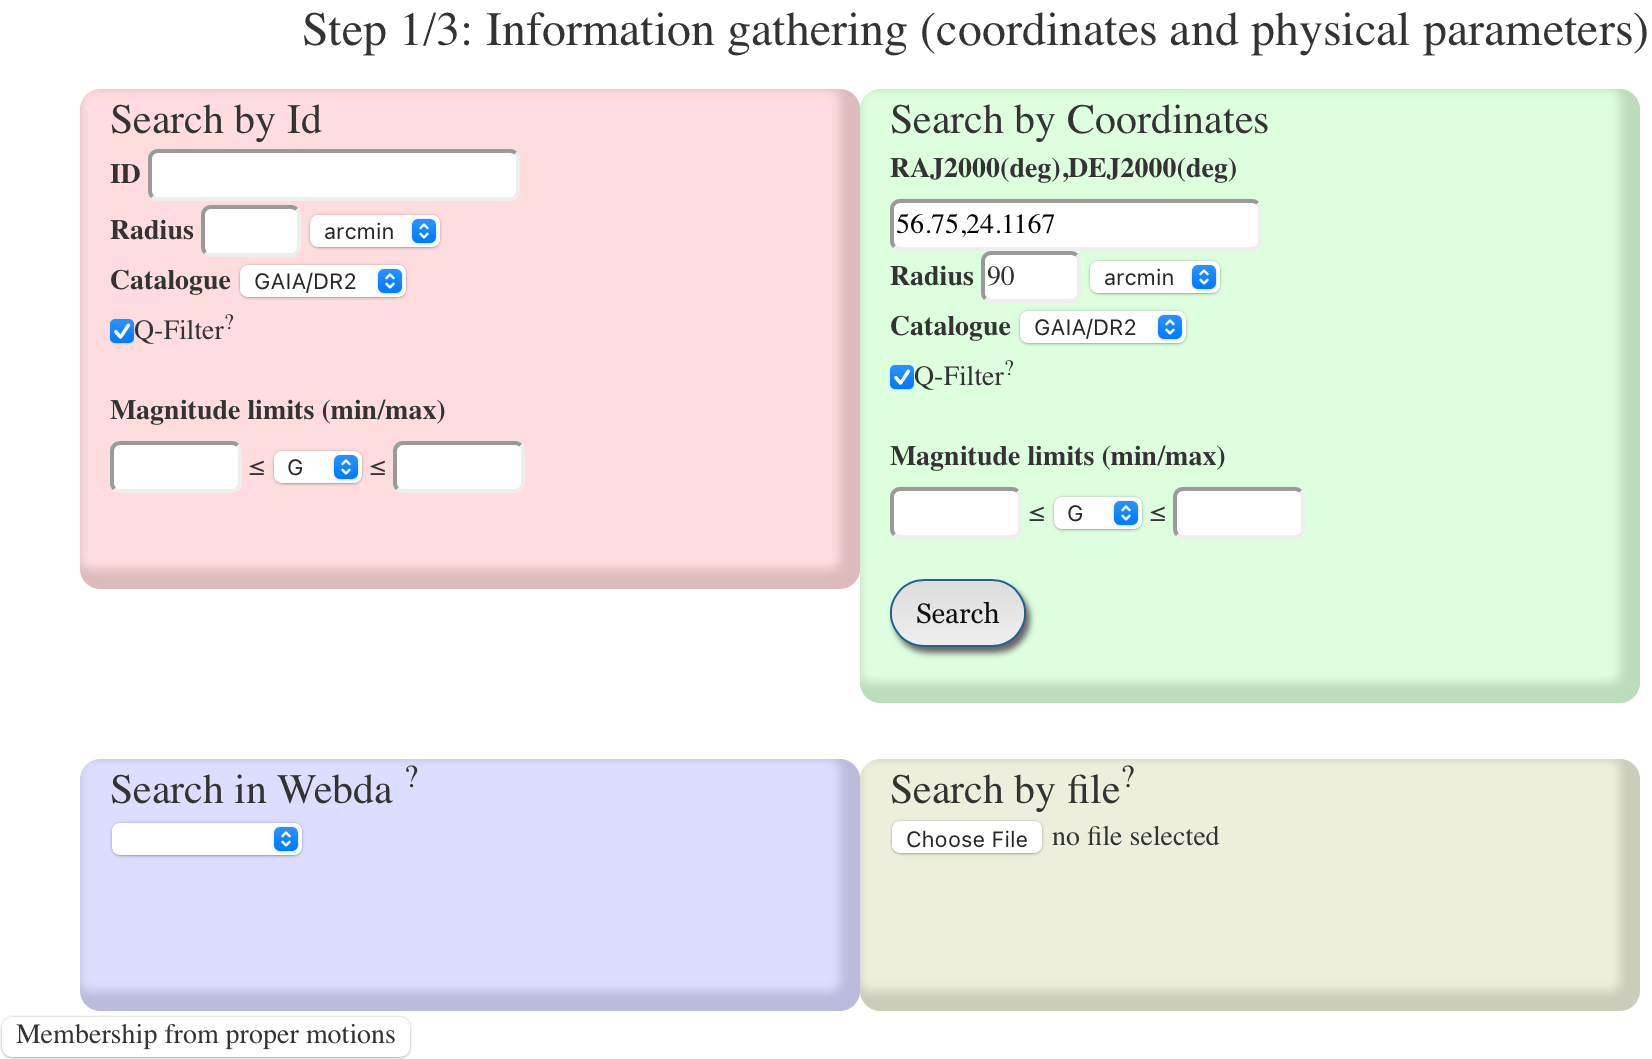
\includegraphics[width=\textwidth]{../figures/clusterix/clusterix_selection_panel_melotte_22.png}
  \end{subfigure}
  \caption{Clusterix 2.0 selection panel with Melotte 22 settings.
           Coordinates correspond to the center of Melotte 22 cluster,
           while the radius is the value registered for this cluster in the
           OpenClust catalogue multiplied by 1.5 (as explained in~\ref{sec:data_mining})}
  \label{fig:clusterix_selection}
\end{figure}

This panel allows us to select a region by its coordinates
or by searching a cluster by its name in the Gaia DR2 catalogue,
as well as to specify the size of the region by introducing its radius.
We can also set limit values in magnitude (for both minimum and maximum)
to discard stars outside these limits.
Another setting is the flag to enable or disable the \emph{Q-Filter}.
This filter discards those stars with \emph{null} values in relevant fields.

Clusterix returns a position map for the downloaded stars from Gaia DR2 database
using Aladin~\cite{bonnarel2000aladin} as an atlas of the sky (See Figure~\ref{fig:aladin_melotte_22}).
At this point, we can choose sending the recovered data to TOPCAT or Aladin,
or continue to the next step of the assistant.

We select the second choice and proceed with the proper motion frequency space analysis.

\begin{figure}[htbp]
  \centering
  \begin{subfigure}{0.9\textwidth}
    \centering
    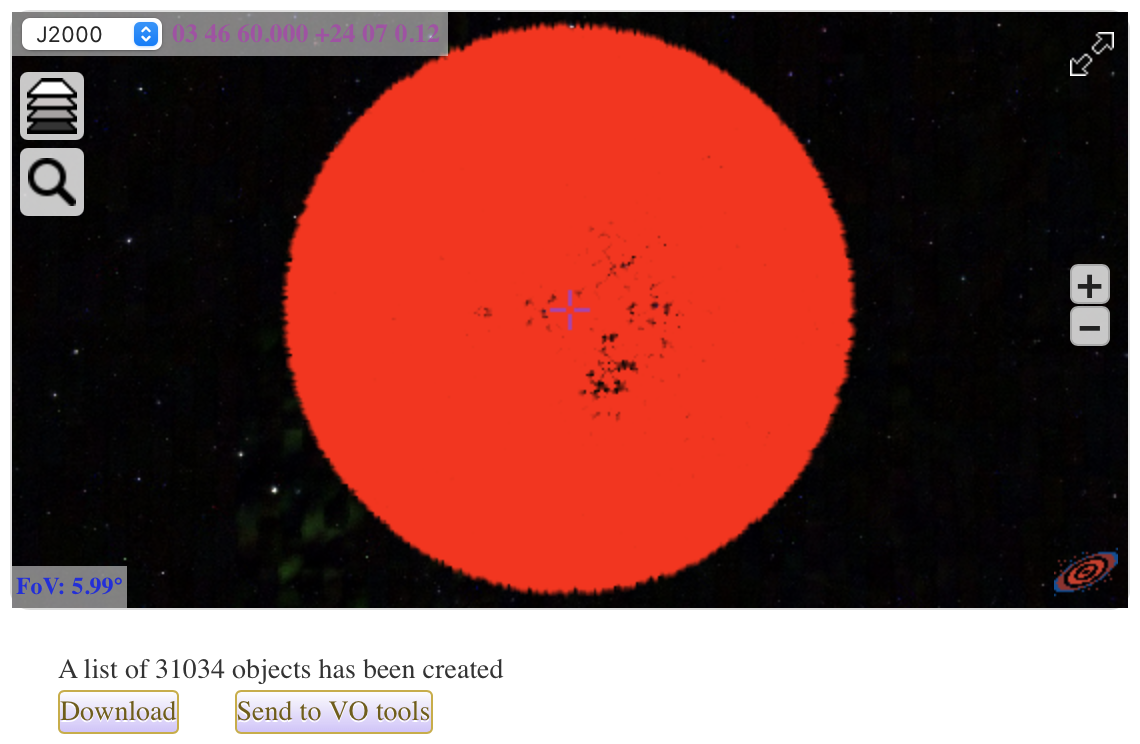
\includegraphics[width=\textwidth]{../figures/clusterix/clusterix_aladin_selection_melotte_22.png}
  \end{subfigure}
  \caption{Aladin screenshot with equatorial coordinates for Melotte 22 stars referred to J2000.}
  \label{fig:aladin_melotte_22}
\end{figure}

In this step, we define three regions that will be used for the frequency analysis:

\begin{itemize}
  \item \textbf{Inner region} (\emph{c+f}), with stars that belong to the OC and field stars.
  \item \textbf{External region} or field region (\emph{f}), with stars that do not belong the open cluster.
  \item \textbf{Void region}. This region is excluded from the analysis since it is supposed
                to be a transition region with stars that could belong the OC.
\end{itemize}

It is necessary to remark the importance of this step,
since the selection of these regions is critical to get a good result.
However, despite how crucial this step is, there is no general rule to define these regions.
We only have two references:
the radius of the downloaded region and the estimated size for the OC that sets the \emph{inner radius}.
The other two radius must be set by trial and error.
In general, they should be large enough to be sure that we are not taking polluted regions.
This is a tedious process and requires several tries before achieving good enough probability values.

Furthermore, it is necessary to know in advance some additional profiles of the cluster,
in addition to the estimated size.
For example, in the case of Melotte 22, the proper motion in declination direction
of the membership stars around \(-45 mas \cdot year^{-1}\),
so it is necessary to open the \(\mu\) range above the estimated values (in absolute value).
If we do not do that we lose the possibility of detection,
since Clusterix sets this value to \(30 mas \cdot year^{-1}\) by default.
But even in this case, it is necessary to set a threshold for magnitude values,
\(G \leq 14\), to help getting the right result.
Figure~\ref{fig:clusterix_step2_melotte_22} shows the region selection panel on Clusterix 2.0.

This makes the selection process an art rather than a science,
not to mention the required previous knowledge on certain profiles of the objects to characterize.
This puts into question the \emph{non-parameterized} character of the validation method.

\begin{figure}[htbp]
  \centering
  \begin{subfigure}{0.9\textwidth}
    \centering
    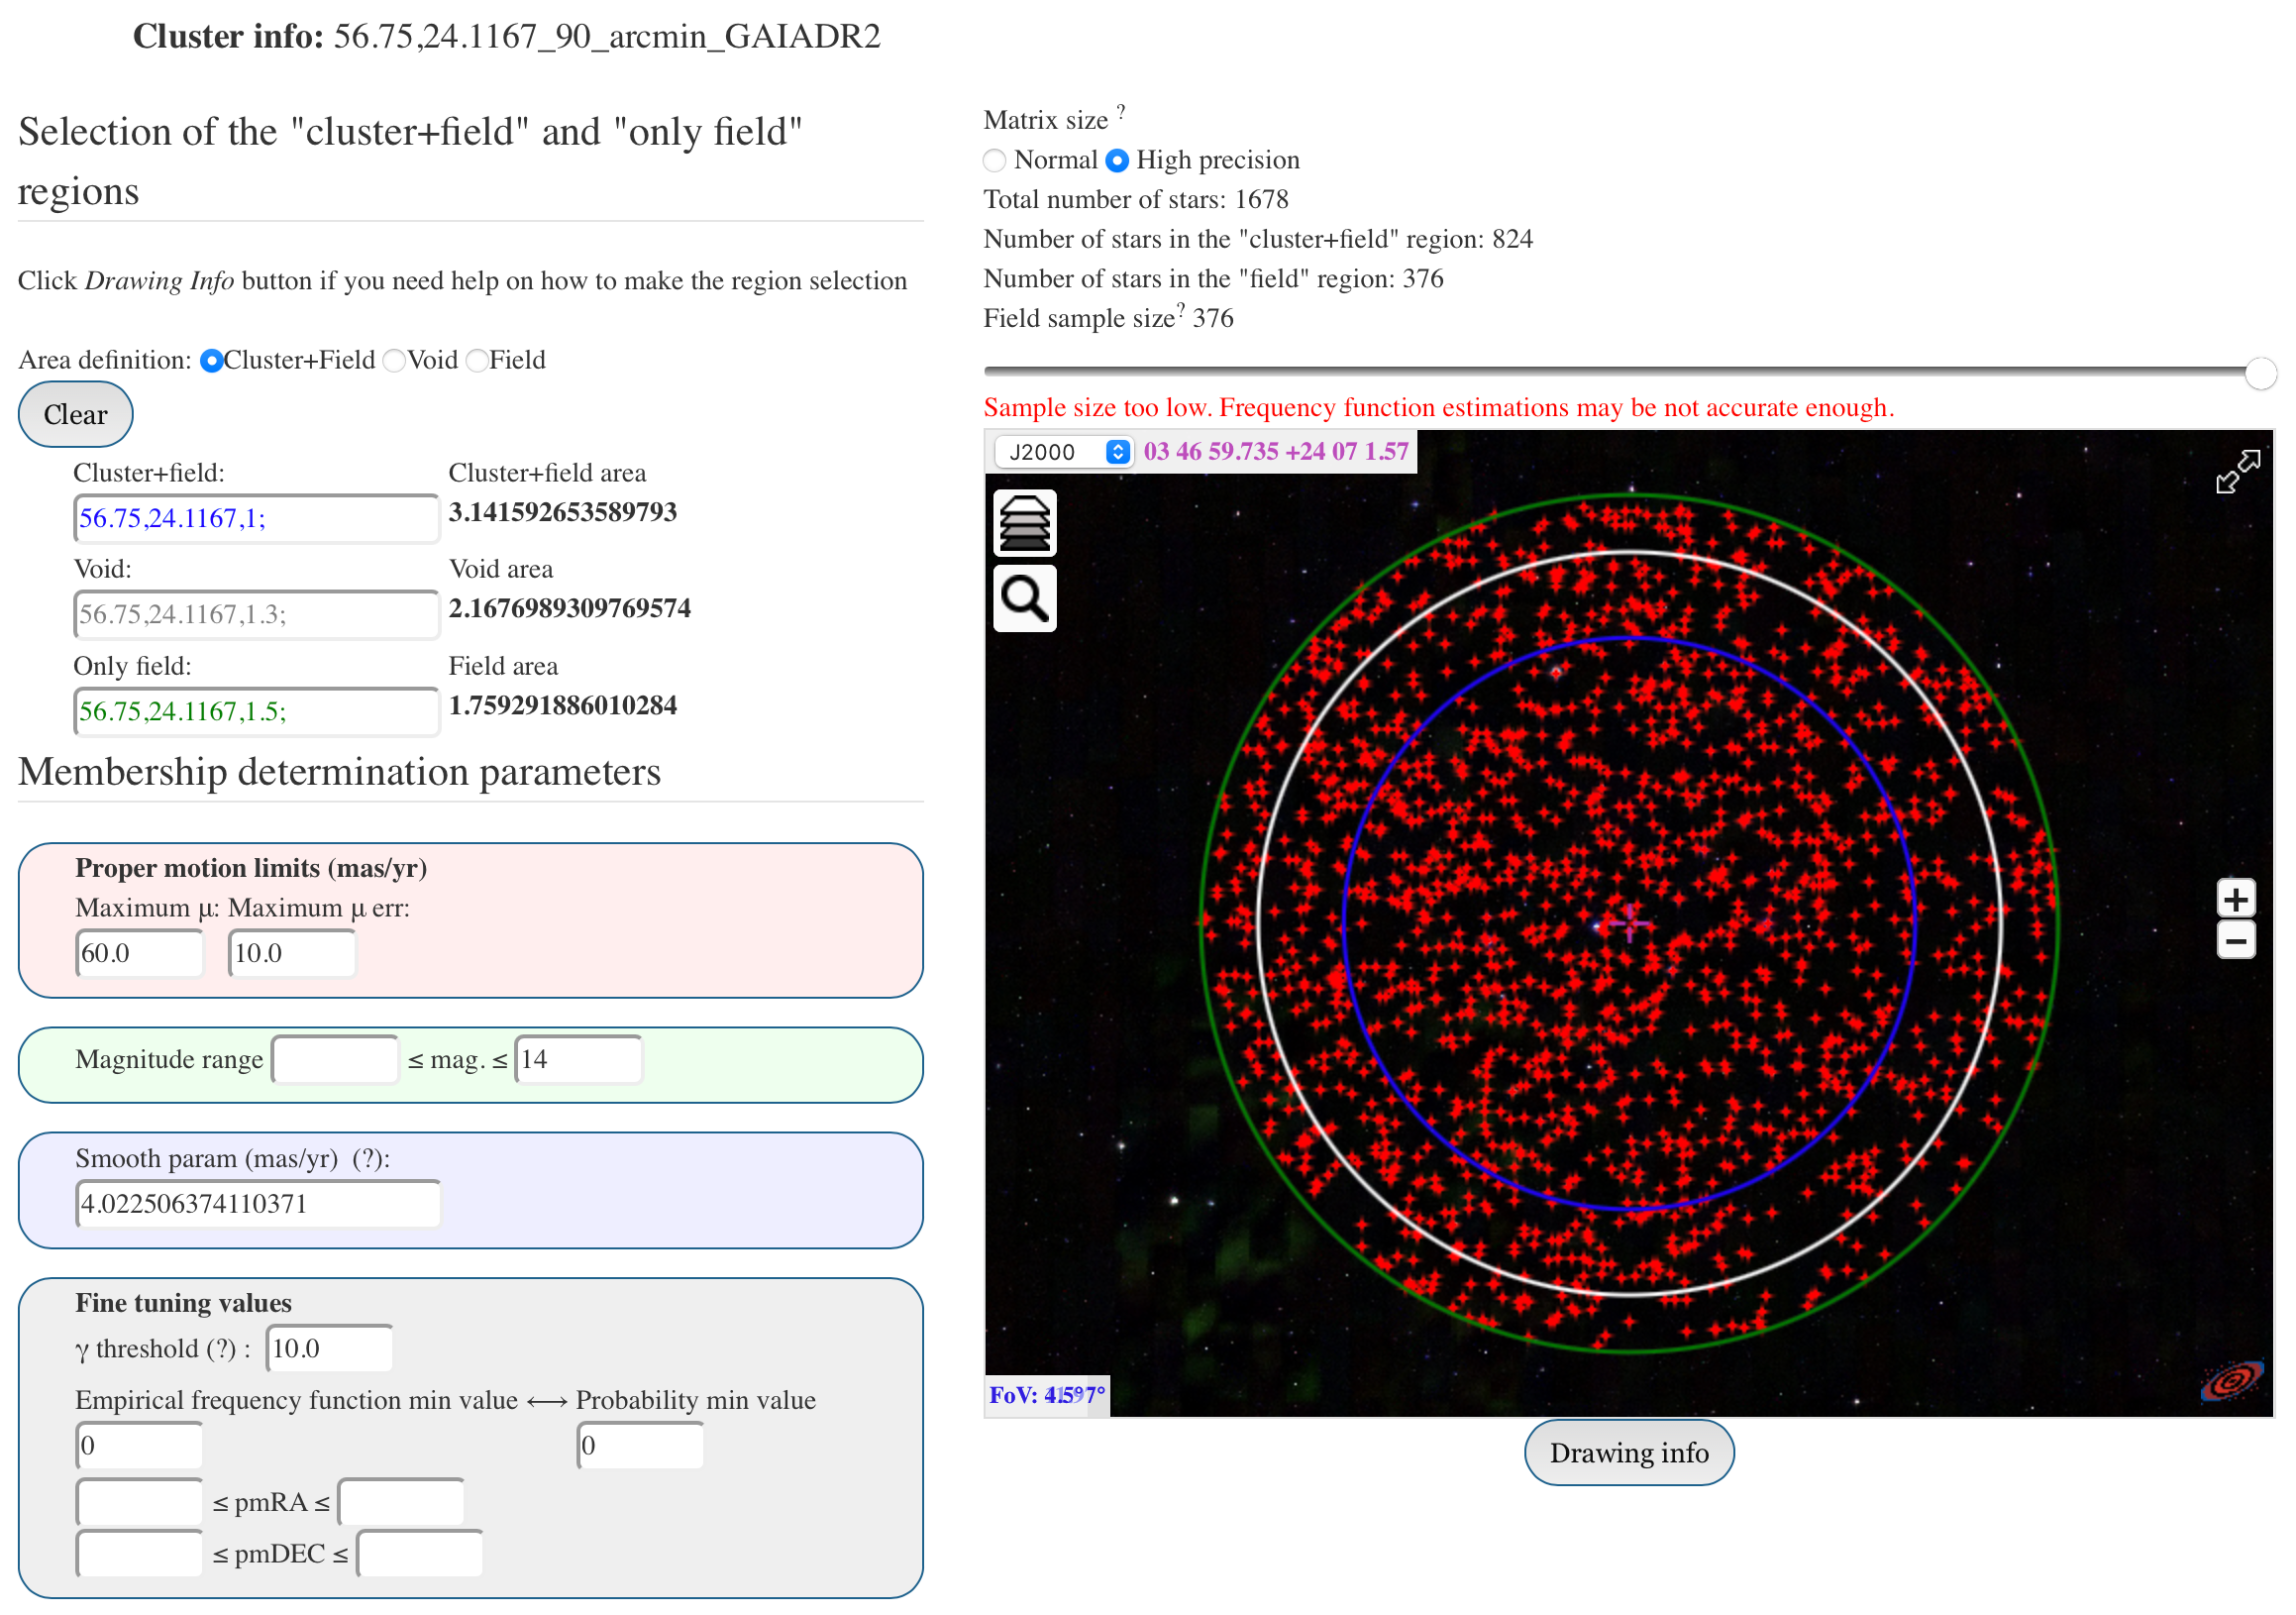
\includegraphics[width=\textwidth]{../figures/clusterix/clusterix_step2_melotte_22.png}
  \end{subfigure}
  \caption{Clusterix 2.0 Step 2/3: Region selection.}
  \label{fig:clusterix_step2_melotte_22}
\end{figure}

After having set all these parameters,
Clusterix performs the proper motion frequency analysis and returns the probability field
associated to each star of the whole region (see Figure~\ref{fig:clusterix_probability_melotte_22}).

This step can be repeated over and over again, varying radii and other parameters,
until finally reach a valid probability that works.
The last step presents a table with candidate objects and allows to export this dataset to TOPCAT,
Aladin and VOSA to perform a deeper filtering and analysis based on the results provided by Clusterix.

\begin{figure}[htbp]
  \centering
  \begin{subfigure}{0.9\textwidth}
    \centering
    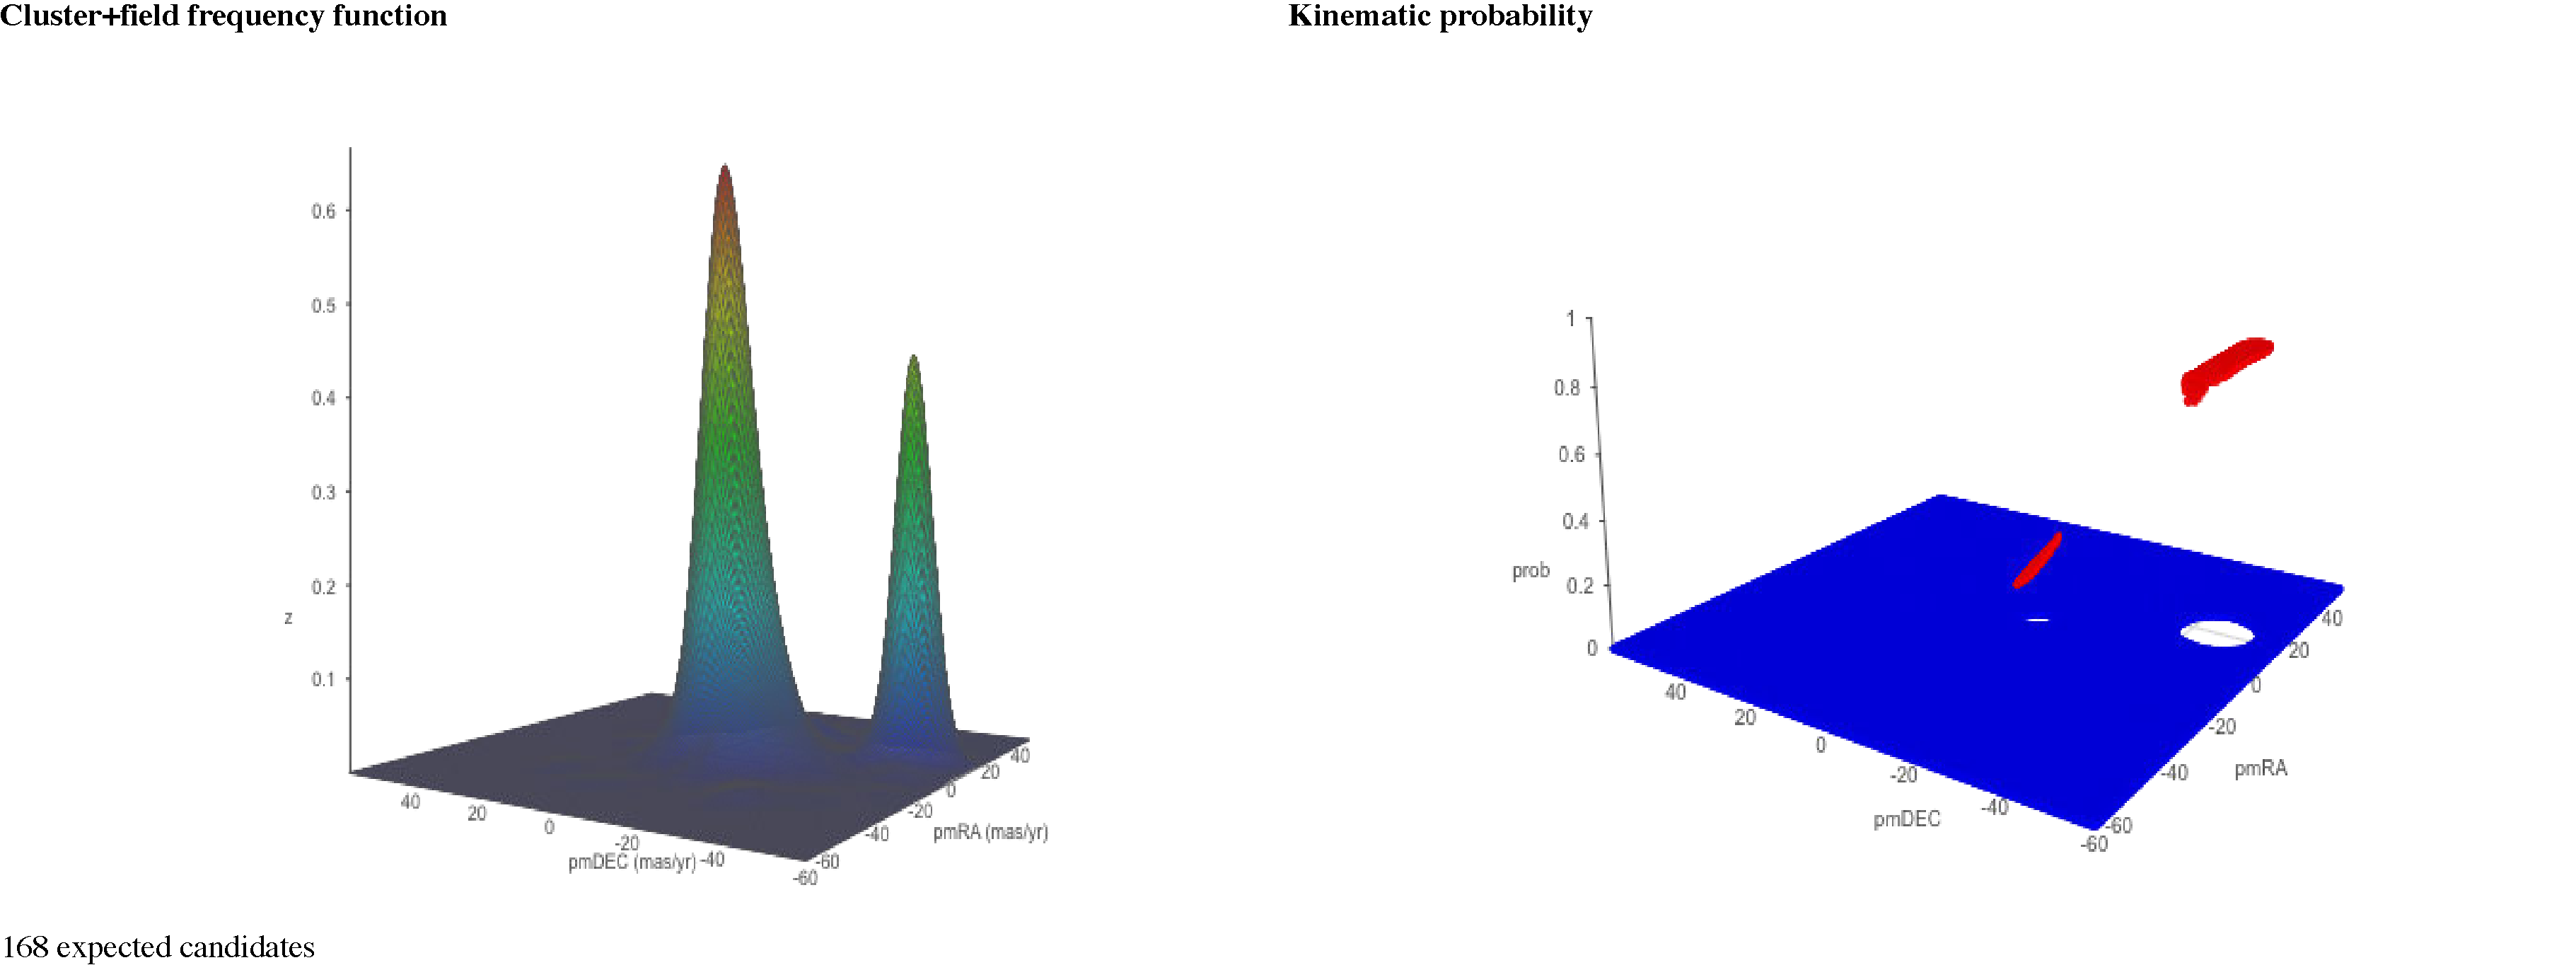
\includegraphics[width=\textwidth]{../figures/clusterix/clusterix_probability_melotte_22.pdf}
  \end{subfigure}
  \caption{Kinematic probability associated to the membership of the open cluster.
           This probability is derived from the proper motion frequency analysis.}
  \label{fig:clusterix_probability_melotte_22}
\end{figure}

Once data is available in TOPCAT, we have to carefully analyze the imported data.
At this point, we can perform a first star selection by excluding those stars with probability value lower than 0.8.
This first result can be taken as a good starting point, but we still need to make some fine tunning.
As we can see in Figure~\ref{fig:topcat_prob_selection_melotte_22},
the selection is too restrictive and we have lost too many stars.

Looking at Figure~\ref{fig:topcat_prob_parallax_melotte_22},
we can assume that cluster members are around \(7.3mas\) in the parallax histogram.
Also, Figure~\ref{fig:topcat_prob_pm_melotte_22} reveals that cluster stars
have low scattering rate in the proper motion configuration space.

\begin{figure}[htbp]
  \centering
  \begin{subfigure}{0.9\textwidth}
    \centering
    \begin{subfigure}[t]{0.45\textwidth}
      \centering
      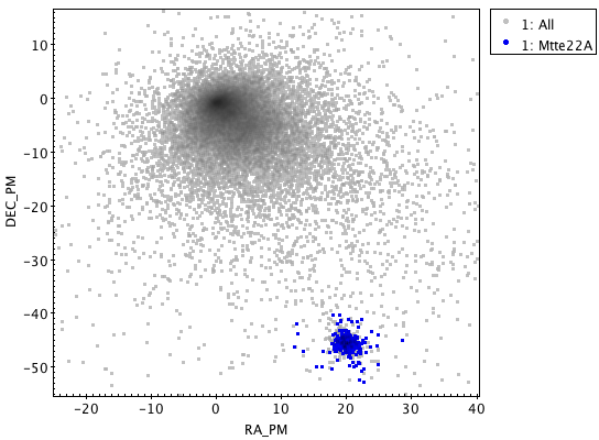
\includegraphics[width=\textwidth]{../figures/clusterix/topcat_prob_pm_melotte_22.png}
      \caption{Proper motion}
      \label{fig:topcat_prob_pm_melotte_22}
    \end{subfigure}
    \hfill
    \begin{subfigure}[t]{0.45\textwidth}
      \centering
      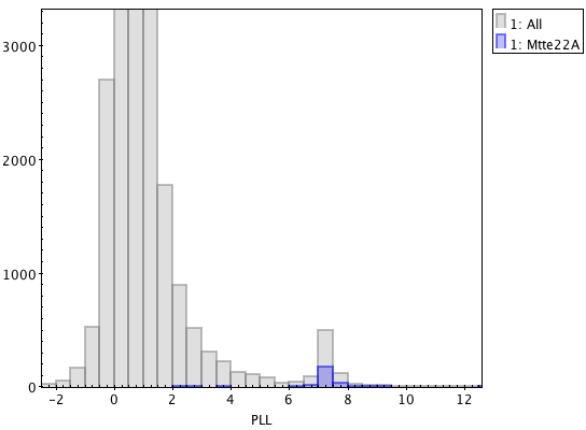
\includegraphics[width=\textwidth]{../figures/clusterix/topcat_prob_parallax_melotte_22.png}
      \caption{Parallax}
      \label{fig:topcat_prob_parallax_melotte_22}
    \end{subfigure}
  \end{subfigure}
  \caption{Melotte 22 first selection using validation method. Parallax is \(7.304mas\) with 0.797 of standard deviation.}
  \label{fig:topcat_prob_selection_melotte_22}
\end{figure}

Taking these observations into account,
we can proceed to make a new selection based on parallax properties.
Our second selection makes use of the values obtained with the previous selection
for parallax and its standard deviation and selects those stars from the whole set
which fall inside the limits \(7.304mas \pm 0.797\) (see Figure~\ref{fig:topcat_parallax_melotte_22}).

\begin{figure}[htbp]
  \centering
  \begin{subfigure}{0.9\textwidth}
    \centering
    \begin{subfigure}[t]{0.45\textwidth}
      \centering
      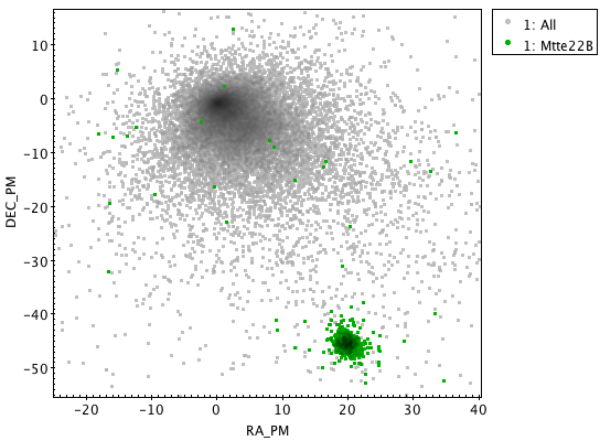
\includegraphics[width=\textwidth]{../figures/clusterix/topcat_2nd_selection_pm_melotte_22.png}
      \caption{Proper motion}
      \label{fig:topcat_2nd_selection_pm_melotte_22}
    \end{subfigure}
    \hfill
    \begin{subfigure}[t]{0.45\textwidth}
      \centering
      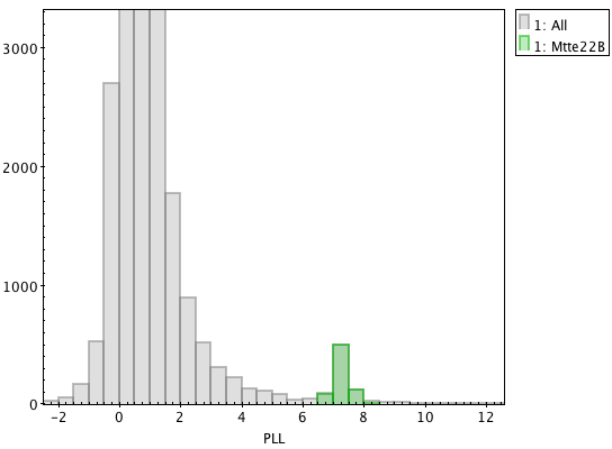
\includegraphics[width=\textwidth]{../figures/clusterix/topcat_2nd_selection_parallax_melotte_22.png}
      \caption{Parallax}
      \label{fig:topcat_2nd_selection_parallax_melotte_22}
    \end{subfigure}
  \end{subfigure}
  \caption{Melotte 22 second selection. The estimated number of cluster members is 709.}
  \label{fig:topcat_parallax_melotte_22}
\end{figure}

Looking at the H-R diagrams (Figure~\ref{fig:clusterix_selection_hr_diagrams_melotte_22}),
we can compare both selections and see how we have extended the selection without
getting too much noise around the isochrone curve.

\begin{figure}[htbp]
  \centering
  \begin{subfigure}{0.9\textwidth}
    \centering
    \begin{subfigure}[t]{0.45\textwidth}
      \centering
      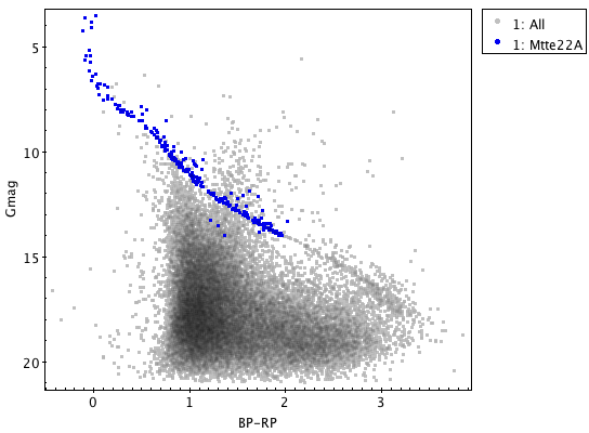
\includegraphics[width=\textwidth]{../figures/clusterix/topcat_1st_selection_hr_diagram_melotte_22.png}
      \caption{H-R diagram from first selection.}
    \end{subfigure}
    \hfill
    \begin{subfigure}[t]{0.45\textwidth}
      \centering
      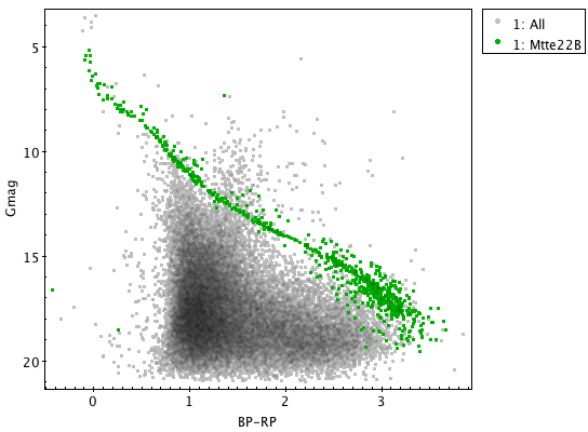
\includegraphics[width=\textwidth]{../figures/clusterix/topcat_2nd_selection_hr_diagram_melotte_22.png}
      \caption{H-R diagram from second selection.}
    \end{subfigure}
  \end{subfigure}
  \caption{Comparison between first and second selection H-R diagrams.}
  \label{fig:clusterix_selection_hr_diagrams_melotte_22}
\end{figure}

Finally, we filter the second selection by discarding those stars whose parallax relative error in absolute value
is behind 0.05 (see Figure~\ref{fig:clusterix_final_selection_melotte_22}).

\begin{figure}[htbp]
  \centering
  \begin{subfigure}{0.9\textwidth}
    \centering
    \begin{subfigure}[t]{0.45\textwidth}
      \centering
      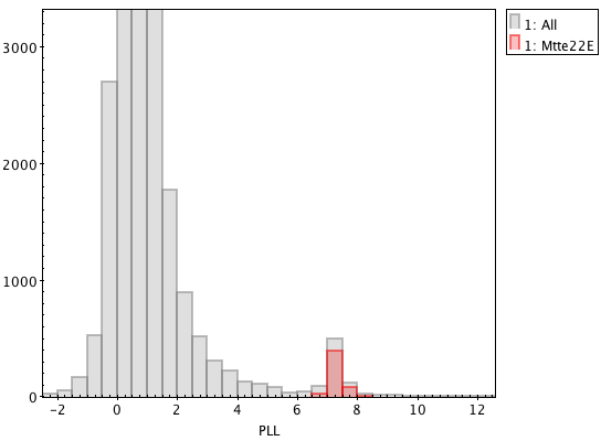
\includegraphics[width=\textwidth]{../figures/clusterix/topcat_3rd_selection_parallax_melotte_22.png}
      \caption{Parallax}
    \end{subfigure}
    \hfill
    \begin{subfigure}[t]{0.45\textwidth}
      \centering
      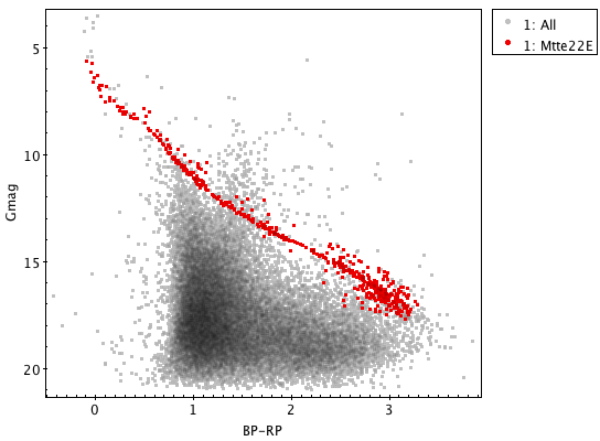
\includegraphics[width=\textwidth]{../figures/clusterix/topcat_3rd_selection_hr_diagram_melotte_22.png}
      \caption{H-R diagram}
    \end{subfigure}
  \end{subfigure}
  \caption{Comparison between first and second selection H-R diagrams.}
  \label{fig:clusterix_final_selection_melotte_22}
\end{figure}

For the sake of completeness, Table~\ref{tab:results_melotte_22} is shown again.
This table summarizes the results obtained with the validation technique and our method.

\begin{table}[h!]
  \begin{center}
    \begin{tabular}{l|c|c|c|c}
      \textbf{Source / method} & \emph{\(\mu_{\alpha}\) \((mas \cdot yr^{-1})\)} & \emph{\(\mu_{\delta}\) \((mas \cdot yr^{-1})\)}
      & \emph{\( \varpi \) \((mas)\)} & \emph{\# stars} \\
      \hline
      \textbf{Simbad.u-strasbg.fr} & 19.997 \( \pm \) 0.127 & -45.548 \( \pm \) 0.101 & 7.364 \( \pm \) 0.005 & 1326 \\
      \textbf{Clusterix+TOPCAT} & 19.98 \( \pm \) 1.25 & -45.47 \( \pm \) 1.48 & 7.33 \( \pm \) 0.21 & 634 \\
      K-Means & 20.25 \( \pm \) 0.95 & -38.01 \( \pm \) 1.08 & 7.23 \( \pm \) 0.06 & 1378 \\
      DEC & 23.67 \( \pm \) 1.29 & -46.23 \( \pm \) 1.50 & 8.04 \( \pm \) 0.09 & 878 \\
      DEC (filtered) & 19.50 \( \pm \) 0.41 & -44.23 \( \pm \) 0.39 & 7.42 \( \pm \) 0.005 & 438 \\
    \end{tabular}
  \end{center}
\end{table}

\section{Comparing and Validating}
\label{sec:comparing_and_validating}

Until now, we have focused our study in the open cluster Melotte 22.
Since our aim is to get a model that fits well for a wide range of clusters,
we will now proceed to show some results obtained for a selection of clusters with different typologies.

All results have been computed with an Apple Mac Pro Late 2013,
2.7GHz 12-Core Intel Xeon E5-2697v2, 64GB RAM 1866MHz DDR3 and two AMD FirePro D700 6GB.
The operative system is macOS BigSur 11.1, with Python 3.8, Keras 2.2 and PlaidML 0.7.

Most executions took a few minutes, while large clusters such as Melotte 25,
took around an hour to perform the calculations.
This is in contrast to~\citeA{castro2020hunting} work,
that used the power of the MareNostrum 42 supercomputer to accomplish its computations.

\newpage

\subsection{NGC 2516}

\begin{figure}[H]
  \centering
  \begin{subfigure}{0.9\textwidth}
    \centering
    \begin{subfigure}[t]{0.30\textwidth}
      \centering
      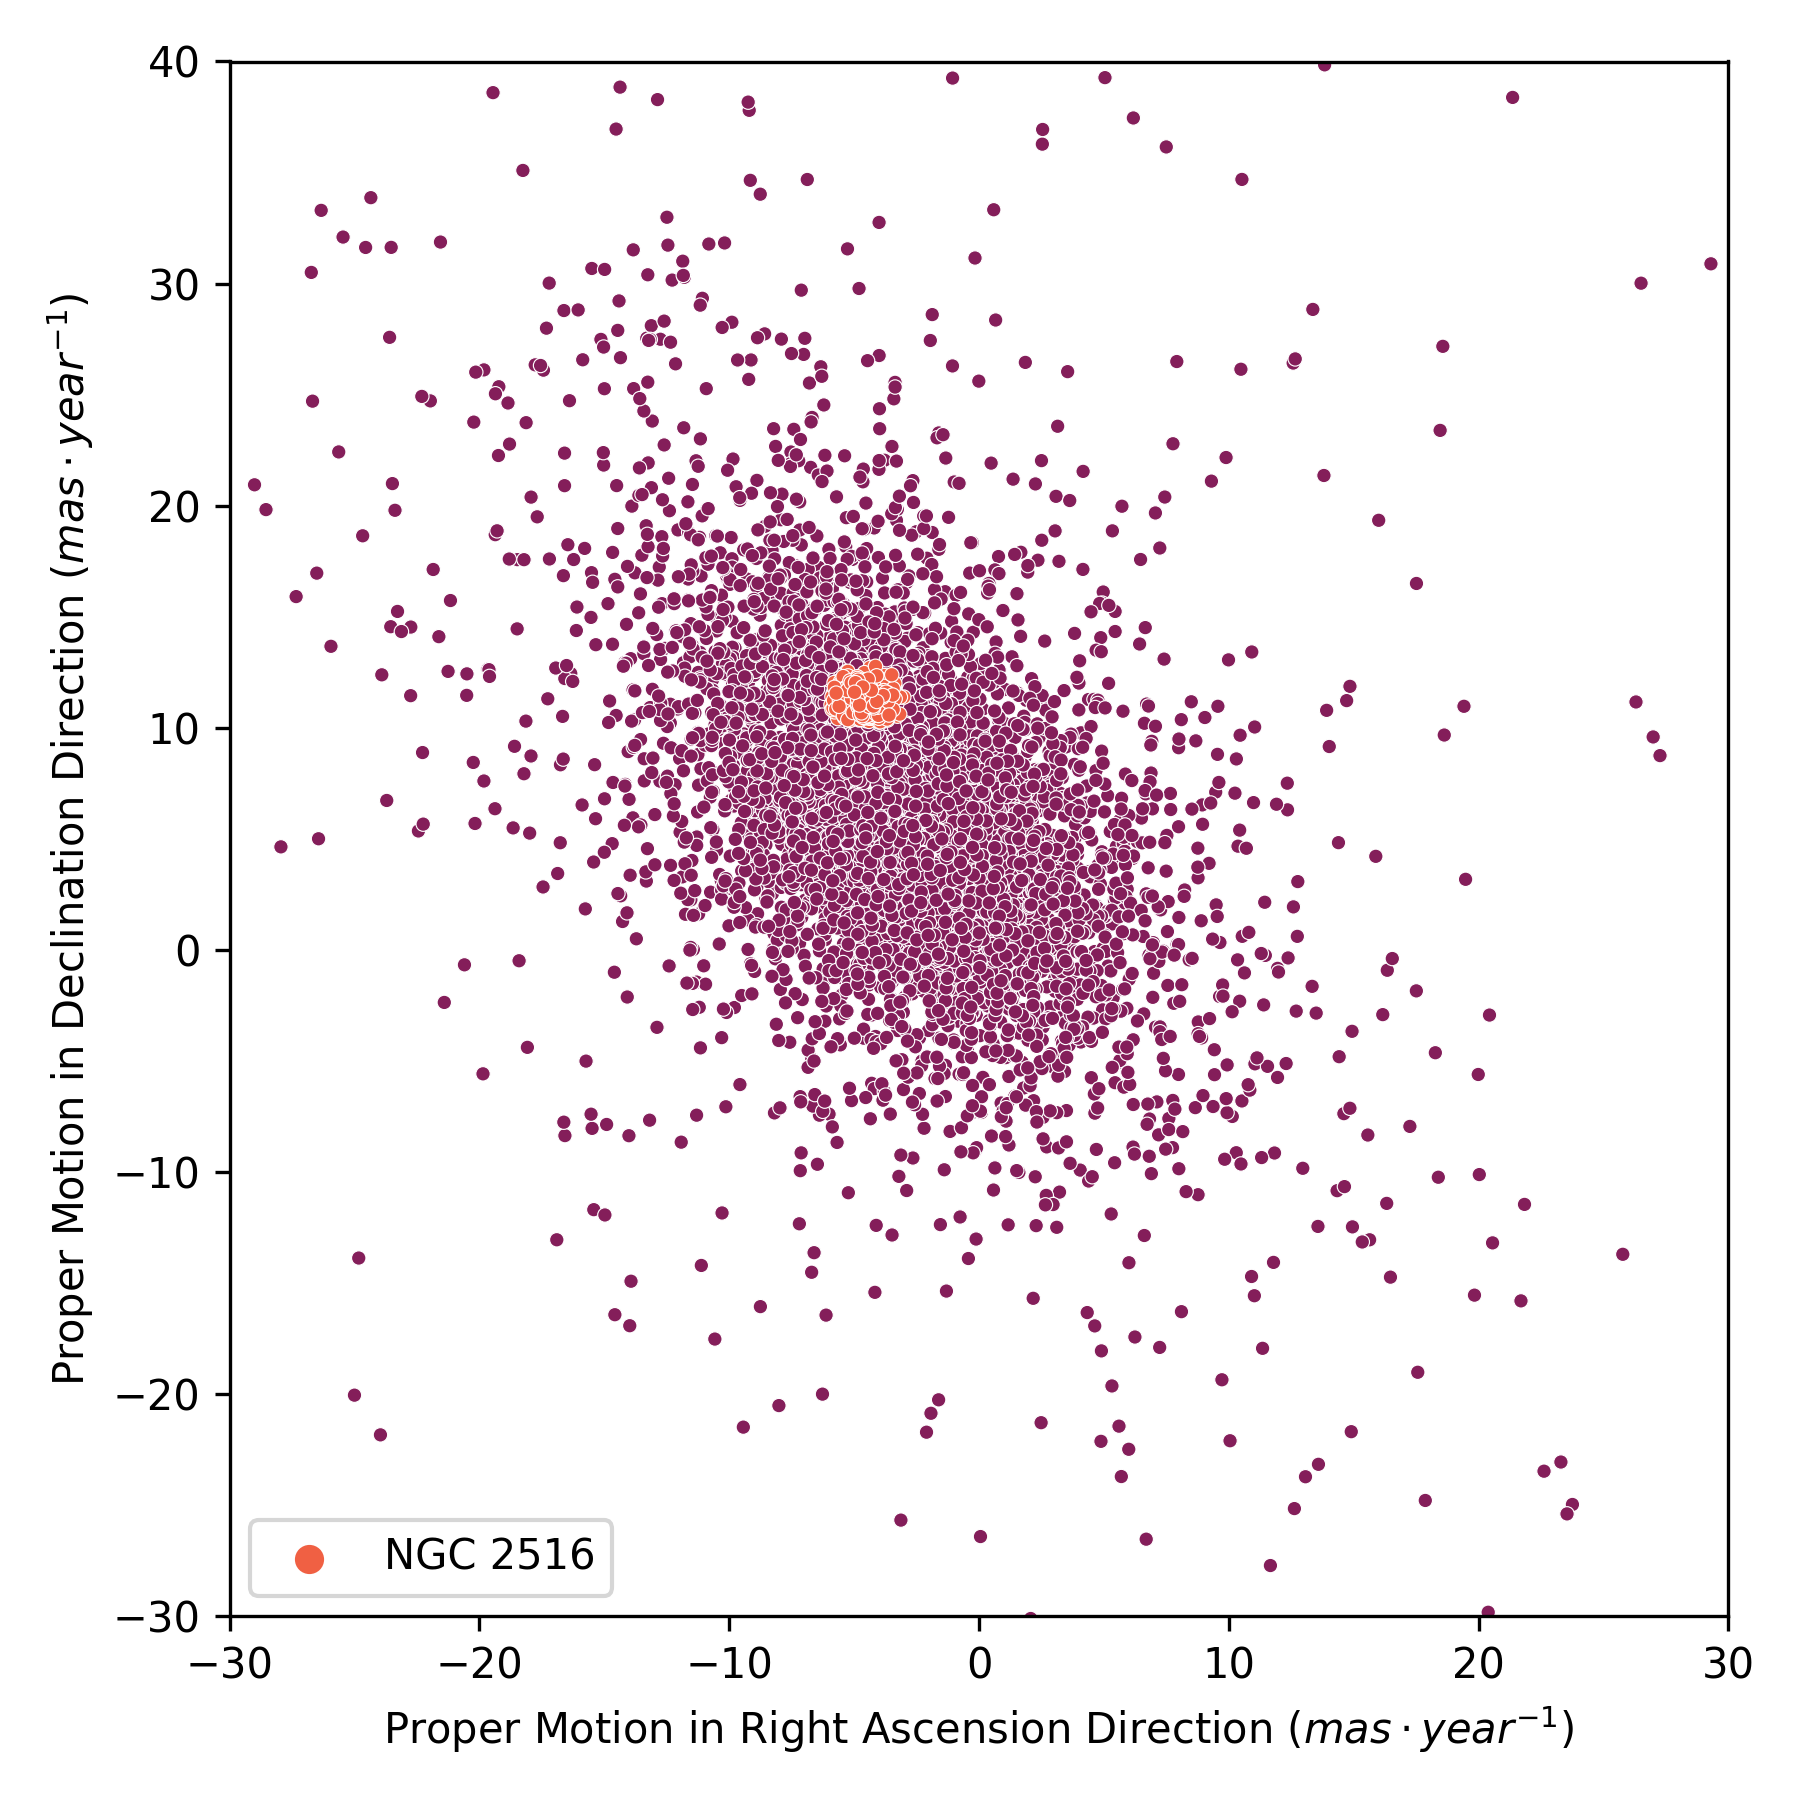
\includegraphics[width=\textwidth]{../figures/ngc_2516/pm_ngc_2516.png}
    \end{subfigure}
    \hfill
    \begin{subfigure}[t]{0.30\textwidth}
      \centering
      \includegraphics[width=\textwidth]{../figures/ngc_2516/parallax_ngc_2516.png}
    \end{subfigure}
    \hfill
    \begin{subfigure}[t]{0.30\textwidth}
      \centering
      \includegraphics[width=\textwidth]{../figures/ngc_2516/hr_diagram_ngc_2516.png}
    \end{subfigure}
  \end{subfigure}
  \caption{NGC 2516 Clusterix+TOPCAT characterization.}
  \label{fig:result_ngc_2516_clusterix}
  \centering
  \begin{subfigure}{0.9\textwidth}
    \centering
    \begin{subfigure}[t]{0.30\textwidth}
      \centering
      \includegraphics[width=\textwidth]{../figures/ngc_2516/kmeans_pm_ngc_2516.png}
    \end{subfigure}
    \hfill
    \begin{subfigure}[t]{0.30\textwidth}
      \centering
      \includegraphics[width=\textwidth]{../figures/ngc_2516/kmeans_parallax_ngc_2516.png}
    \end{subfigure}
    \hfill
    \begin{subfigure}[t]{0.30\textwidth}
      \centering
      \includegraphics[width=\textwidth]{../figures/ngc_2516/kmeans_hr_diagram_ngc_2516.png}
    \end{subfigure}
  \end{subfigure}
  \caption{NGC 2516 K-Means characterization. Identified as cluster \emph{g3}.}
  \label{fig:result_ngc_2516_kmeans}
  \centering
  \begin{subfigure}{0.9\textwidth}
    \centering
    \begin{subfigure}[t]{0.30\textwidth}
      \centering
      \includegraphics[width=\textwidth]{../figures/ngc_2516/dec_pm_ngc_2516.png}
    \end{subfigure}
    \hfill
    \begin{subfigure}[t]{0.30\textwidth}
      \centering
      \includegraphics[width=\textwidth]{../figures/ngc_2516/dec_parallax_ngc_2516.png}
    \end{subfigure}
    \hfill
    \begin{subfigure}[t]{0.30\textwidth}
      \centering
      \includegraphics[width=\textwidth]{../figures/ngc_2516/dec_hr_diagram_ngc_2516.png}
    \end{subfigure}
  \end{subfigure}
  \caption{NGC 2516 DEC characterization. Identified as cluster \emph{g3}.}
  \label{fig:result_ngc_2516_dec}
  \centering
  \begin{subfigure}{0.9\textwidth}
    \centering
    \begin{subfigure}[t]{0.30\textwidth}
      \centering
      \includegraphics[width=\textwidth]{../figures/ngc_2516/dec_pm_filtered_ngc_2516.png}
    \end{subfigure}
    \hfill
    \begin{subfigure}[t]{0.30\textwidth}
      \centering
      \includegraphics[width=\textwidth]{../figures/ngc_2516/dec_parallax_filtered_ngc_2516.png}
    \end{subfigure}
    \hfill
    \begin{subfigure}[t]{0.30\textwidth}
      \centering
      \includegraphics[width=\textwidth]{../figures/ngc_2516/dec_hr_diagram_filtered_ngc_2516.png}
    \end{subfigure}
  \end{subfigure}
  \caption{NGC 2516 DEC (filtered) characterization. Identified as cluster \emph{g3}.}
  \label{fig:result_ngc_2516_dec_filtered}
\end{figure}

\newpage

Figure~\ref{fig:result_ngc_2516_clusterix} shows NGC 2516 characterized using Clusterix+TOPCAT tools.
Figure~\ref{fig:result_ngc_2516_kmeans} shows eight clusters identified by K-Means.
In this case, cluster \emph{g3} is the one we are looking for.
Figures~\ref{fig:result_ngc_2516_dec} and~\ref{fig:result_ngc_2516_dec_filtered}
show the groups found using the DEC model and the DEC model filtered, respectively.
Again, the cluster of interest is the group \emph{g3}.
Although in general, groups between K-Means model and DEC models may not match.

Table~\ref{tab:hyperparameters_ngc_2516} shows the hyperparameters used for characterizing NGC 2516
with the DEC model. Table~\ref{tab:results_ngc_2516} shows a results summary for NGC 2516.

\vfill

\begin{table}[h]
  \begin{center}
    \begin{tabular}{l|c}
      \textbf{Hyperparameter} & \textbf{Value} \\
      \hline
      Number of Clusters & 8 \\
      Clustering Layer & \(\left[ 50, 50, 60 \right]\) \\
      Kernel Initializer Seed & 2 \\
      Quantil Threshold & 0.15 \\
    \end{tabular}
    \caption{NGC 2516 DEC model hyperparameters.}
    \label{tab:hyperparameters_ngc_2516}
  \end{center}
\end{table}

\vfill

\begin{table}[h]
  \begin{center}
    \begin{tabular}{l|c|c|c|c}
      \textbf{Source / method} & \emph{\(\mu_{\alpha}\) \((mas \cdot yr^{-1})\)} & \emph{\(\mu_{\delta}\) \((mas \cdot yr^{-1})\)}
      & \emph{\( \varpi \) \((mas)\)} & \emph{\# stars} \\
      \hline
      \textbf{Simbad.u-strasbg.fr} & -4.6579 \( \pm \) 0.0075 & 11.1517 \( \pm \) 0.0075 & 2.4118 \( \pm \) 0.0006 & 1727 \\
      Clusterix+TOPCAT & -4.652 \( \pm \) 0.523 & 11.203 \( \pm \) 0.454 & 2.409 \( \pm \) 0.127 & 638 \\
      K-Means & -4.344 \( \pm \) 0.14 & 9.507 \( \pm \) 0.19 & 2.268 \( \pm \) 0.01 & 1542 \\
      DEC & -4.426 \( \pm \) 0.17 & 9.952 \( \pm \) 0.20 & 2.436 \( \pm \) 0.01 & 1532 \\
      \textbf{DEC (filtered)} & -4.502 \( \pm \) 0.14 & 10.114 \( \pm \) 0.17 & 2.392 \( \pm \) 0.004 & 1072 \\
    \end{tabular}
    \caption{NGC 2516 results.}
    \label{tab:results_ngc_2516}
  \end{center}
\end{table}

\vfill

\newpage

\subsection{NGC 2632}

\begin{figure}[H]
  \vfil
  \centering
  \begin{subfigure}{0.9\textwidth}
    \centering
    \begin{subfigure}[t]{0.30\textwidth}
      \centering
      \includegraphics[width=\textwidth]{../figures/ngc_2632/pm_ngc_2632.png}
    \end{subfigure}
    \hfill
    \begin{subfigure}[t]{0.30\textwidth}
      \centering
      \includegraphics[width=\textwidth]{../figures/ngc_2632/parallax_ngc_2632.png}
    \end{subfigure}
    \hfill
    \begin{subfigure}[t]{0.30\textwidth}
      \centering
      \includegraphics[width=\textwidth]{../figures/ngc_2632/hr_diagram_ngc_2632.png}
    \end{subfigure}
  \end{subfigure}
  \caption{NGC 2632 Clusterix+TOPCAT characterization.}
  \label{fig:result_ngc_2632_clusterix}
  \centering
  \begin{subfigure}{0.9\textwidth}
    \centering
    \begin{subfigure}[t]{0.30\textwidth}
      \centering
      \includegraphics[width=\textwidth]{../figures/ngc_2632/kmeans_pm_ngc_2632.png}
    \end{subfigure}
    \hfill
    \begin{subfigure}[t]{0.30\textwidth}
      \centering
      \includegraphics[width=\textwidth]{../figures/ngc_2632/kmeans_parallax_ngc_2632.png}
    \end{subfigure}
    \hfill
    \begin{subfigure}[t]{0.30\textwidth}
      \centering
      \includegraphics[width=\textwidth]{../figures/ngc_2632/kmeans_hr_diagram_ngc_2632.png}
    \end{subfigure}
  \end{subfigure}
  \caption{NGC 2632 K-Means characterization. Identified as cluster \emph{g1}.}
  \label{fig:result_ngc_2632_kmeans}
  \centering
  \begin{subfigure}{0.9\textwidth}
    \centering
    \begin{subfigure}[t]{0.30\textwidth}
      \centering
      \includegraphics[width=\textwidth]{../figures/ngc_2632/dec_pm_ngc_2632.png}
    \end{subfigure}
    \hfill
    \begin{subfigure}[t]{0.30\textwidth}
      \centering
      \includegraphics[width=\textwidth]{../figures/ngc_2632/dec_parallax_ngc_2632.png}
    \end{subfigure}
    \hfill
    \begin{subfigure}[t]{0.30\textwidth}
      \centering
      \includegraphics[width=\textwidth]{../figures/ngc_2632/dec_hr_diagram_ngc_2632.png}
    \end{subfigure}
  \end{subfigure}
  \caption{NGC 2632 DEC characterization. Identified as cluster \emph{g1}.}
  \label{fig:result_ngc_2632_dec}
  \centering
  \begin{subfigure}{0.9\textwidth}
    \centering
    \begin{subfigure}[t]{0.30\textwidth}
      \centering
      \includegraphics[width=\textwidth]{../figures/ngc_2632/dec_pm_filtered_ngc_2632.png}
    \end{subfigure}
    \hfill
    \begin{subfigure}[t]{0.30\textwidth}
      \centering
      \includegraphics[width=\textwidth]{../figures/ngc_2632/dec_parallax_filtered_ngc_2632.png}
    \end{subfigure}
    \hfill
    \begin{subfigure}[t]{0.30\textwidth}
      \centering
      \includegraphics[width=\textwidth]{../figures/ngc_2632/dec_hr_diagram_filtered_ngc_2632.png}
    \end{subfigure}
  \end{subfigure}
  \caption{NGC 2632 DEC (filtered) characterization. Identified as cluster \emph{g1}.}
  \label{fig:result_ngc_2632_dec_filtered}
\end{figure}

\newpage

Figure~\ref{fig:result_ngc_2632_clusterix} shows NGC 2632 characterized by the validation method.
Figure~\ref{fig:result_ngc_2632_kmeans} shows ten clusters identified by K-Means.
Cluster \emph{g1} is the open cluster we are looking for.
Figures~\ref{fig:result_ngc_2632_dec} and~\ref{fig:result_ngc_2632_dec_filtered}
show the groups found using the DEC model and the DEC model filtered, respectively.
Open cluster NGC 2632 is labeled as group \emph{g1}.

Table~\ref{tab:hyperparameters_ngc_2632} shows the hyperparameters used for characterizing NGC 2632
with our model. Table~\ref{tab:results_ngc_2632} shows a results summary for NGC 2632 analysis.

\vfill

\begin{table}[h]
  \begin{center}
    \begin{tabular}{l|c}
      \textbf{Hyperparameter} & \textbf{Value} \\
      \hline
      Number of Clusters & 10 \\
      Clustering Layer & \(\left[ 50, 50, 40 \right]\) \\
      Kernel Initializer Seed & 10 \\
      Quantil Threshold & 0.1 \\
    \end{tabular}
    \caption{NGC 2632 DEC model hyperparameters.}
    \label{tab:hyperparameters_ngc_2632}
  \end{center}
\end{table}

\vfill

\begin{table}[h]
  \begin{center}
    \begin{tabular}{l|c|c|c|c}
      \textbf{Source / method} & \emph{\(\mu_{\alpha}\) \((mas \cdot yr^{-1})\)} & \emph{\(\mu_{\delta}\) \((mas \cdot yr^{-1})\)}
      & \emph{\( \varpi \) \((mas)\)} & \emph{\# stars} \\
      \hline
      \textbf{Simbad.u-strasbg.fr} & -36.047 \( \pm \) 0.110 & -12.917 \( \pm \) 0.066 & 5.371 \( \pm \) 0.003 & - \\
      Clusterix+TOPCAT & -36.154 \( \pm \) 1.001 & -12.909 \( \pm \) 0.806 & 5.327 \( \pm \) 0.187 & 371 \\
      K-Means & -26.352 \( \pm \) 0.82 & -15.828 \( \pm \) 0.76 & 5.394 \( \pm \) 0.03 & 629 \\
      DEC & -20.012 \( \pm \) 0.69 & -14.742 \( \pm \) 0.58 & 4.686 \( \pm \) 0.03 & 894 \\
      \textbf{DEC (filtered)} & -21.571 \( \pm \) 0.74 & -14.234 \( \pm \) 0.61 & 4.719 \( \pm \) 0.03 & 714 \\
    \end{tabular}
    \caption{NGC 2632 results.}
    \label{tab:results_ngc_2632}
  \end{center}
\end{table}

\vfill

\newpage

\subsection{NGC 2682}

\begin{figure}[H]
  \vfil
  \centering
  \begin{subfigure}{0.9\textwidth}
    \centering
    \begin{subfigure}[t]{0.30\textwidth}
      \centering
      \includegraphics[width=\textwidth]{../figures/ngc_2682/pm_ngc_2682.png}
    \end{subfigure}
    \hfill
    \begin{subfigure}[t]{0.30\textwidth}
      \centering
      \includegraphics[width=\textwidth]{../figures/ngc_2682/parallax_ngc_2682.png}
    \end{subfigure}
    \hfill
    \begin{subfigure}[t]{0.30\textwidth}
      \centering
      \includegraphics[width=\textwidth]{../figures/ngc_2682/hr_diagram_ngc_2682.png}
    \end{subfigure}
  \end{subfigure}
  \caption{NGC 2682 Clusterix+TOPCAT characterization.}
  \label{fig:result_ngc_2682_clusterix}
  \centering
  \begin{subfigure}{0.9\textwidth}
    \centering
    \begin{subfigure}[t]{0.30\textwidth}
      \centering
      \includegraphics[width=\textwidth]{../figures/ngc_2682/kmeans_pm_ngc_2682.png}
    \end{subfigure}
    \hfill
    \begin{subfigure}[t]{0.30\textwidth}
      \centering
      \includegraphics[width=\textwidth]{../figures/ngc_2682/kmeans_parallax_ngc_2682.png}
    \end{subfigure}
    \hfill
    \begin{subfigure}[t]{0.30\textwidth}
      \centering
      \includegraphics[width=\textwidth]{../figures/ngc_2682/kmeans_hr_diagram_ngc_2682.png}
    \end{subfigure}
  \end{subfigure}
  \caption{NGC 2682 K-Means characterization. Identified as cluster \emph{g4}.}
  \label{fig:result_ngc_2682_kmeans}
  \centering
  \begin{subfigure}{0.9\textwidth}
    \centering
    \begin{subfigure}[t]{0.30\textwidth}
      \centering
      \includegraphics[width=\textwidth]{../figures/ngc_2682/dec_pm_ngc_2682.png}
    \end{subfigure}
    \hfill
    \begin{subfigure}[t]{0.30\textwidth}
      \centering
      \includegraphics[width=\textwidth]{../figures/ngc_2682/dec_parallax_ngc_2682.png}
    \end{subfigure}
    \hfill
    \begin{subfigure}[t]{0.30\textwidth}
      \centering
      \includegraphics[width=\textwidth]{../figures/ngc_2682/dec_hr_diagram_ngc_2682.png}
    \end{subfigure}
  \end{subfigure}
  \caption{NGC 2682 DEC characterization. Identified as cluster \emph{g2}.}
  \label{fig:result_ngc_2682_dec}
  \centering
  \begin{subfigure}{0.9\textwidth}
    \centering
    \begin{subfigure}[t]{0.30\textwidth}
      \centering
      \includegraphics[width=\textwidth]{../figures/ngc_2682/dec_pm_filtered_ngc_2682.png}
    \end{subfigure}
    \hfill
    \begin{subfigure}[t]{0.30\textwidth}
      \centering
      \includegraphics[width=\textwidth]{../figures/ngc_2682/dec_parallax_filtered_ngc_2682.png}
    \end{subfigure}
    \hfill
    \begin{subfigure}[t]{0.30\textwidth}
      \centering
      \includegraphics[width=\textwidth]{../figures/ngc_2682/dec_hr_diagram_filtered_ngc_2682.png}
    \end{subfigure}
  \end{subfigure}
  \caption{NGC 2682 DEC (filtered) characterization. Identified as cluster \emph{g2}.}
  \label{fig:result_ngc_2682_dec_filtered}
\end{figure}

\newpage

Figure~\ref{fig:result_ngc_2682_clusterix} shows NGC 2682 characterized using Clusterix+TOPCAT tools.
Figure~\ref{fig:result_ngc_2682_kmeans} shows ten clusters identified by K-Means.
K-Means labels NGC 2682 as group \emph{g4}.
Figures~\ref{fig:result_ngc_2682_dec} and~\ref{fig:result_ngc_2682_dec_filtered}
show the groups found using the DEC model and the DEC model filtered, respectively.
The cluster of interest is the group \emph{g2}.

Table~\ref{tab:hyperparameters_ngc_2682} shows the hyperparameters used for characterizing NGC 2682
with the DEC model. Table~\ref{tab:results_ngc_2682} shows a results summary for NGC 2682.

\vfill

\begin{table}[h]
  \begin{center}
    \begin{tabular}{l|c}
      \textbf{Hyperparameter} & \textbf{Value} \\
      \hline
      Number of Clusters & 10 \\
      Clustering Layer & \(\left[ 50, 50, 40 \right]\) \\
      Kernel Initializer Seed & 0 \\
      Quantil Threshold & 0.1 \\
    \end{tabular}
    \caption{NGC 2682 DEC model hyperparameters.}
    \label{tab:hyperparameters_ngc_2682}
  \end{center}
\end{table}

\vfill

\begin{table}[h]
  \begin{center}
    \begin{tabular}{l|c|c|c|c}
      \textbf{Source / method} & \emph{\(\mu_{\alpha}\) \((mas \cdot yr^{-1})\)} & \emph{\(\mu_{\delta}\) \((mas \cdot yr^{-1})\)}
      & \emph{\( \varpi \) \((mas)\)} & \emph{\# stars} \\
      \hline
      \textbf{Simbad.u-strasbg.fr} & -10.9737 \( \pm \) 0.0064 & -2.9396 \( \pm \) 0.0063 & 1.1325 \( \pm \) 0.0011 & 1194 \\
      Clusterix+TOPCAT & -10.970 \( \pm \) 0.322 & -2.958 \( \pm \) 0.327 & 1.142 \( \pm \) 0.080 & 649 \\
      K-Means & -8.616 \( \pm \) 0.15 & -3.710 \( \pm \) 0.16 & 1.196 \( \pm \) 0.01 & 1374 \\
      DEC & -8.926 \( \pm \) 0.15 & -3.550 \( \pm \) 0.15 & 1.144 \( \pm \) 0.005 & 1238 \\
      \textbf{DEC (filtered)} & -9.619 \( \pm \) 0.13 & -3.317 \( \pm \) 0.13 & 1.140 \( \pm \) 0.003 & 990 \\
    \end{tabular}
    \caption{NGC 2682 results.}
    \label{tab:results_ngc_2682}
  \end{center}
\end{table}

\vfill

\newpage

\subsection{Melotte 25}

\begin{figure}[H]
  \vfil
  \centering
  \begin{subfigure}{0.9\textwidth}
    \centering
    \begin{subfigure}[t]{0.30\textwidth}
      \centering
      \includegraphics[width=\textwidth]{../figures/melotte_25/pm_melotte_25.png}
    \end{subfigure}
    \hfill
    \begin{subfigure}[t]{0.30\textwidth}
      \centering
      \includegraphics[width=\textwidth]{../figures/melotte_25/parallax_melotte_25.png}
    \end{subfigure}
    \hfill
    \begin{subfigure}[t]{0.30\textwidth}
      \centering
      \includegraphics[width=\textwidth]{../figures/melotte_25/hr_diagram_melotte_25.png}
    \end{subfigure}
  \end{subfigure}
  \caption{Melotte 25 Clusterix+TOPCAT characterization.}
  \label{fig:result_melotte_25_clusterix}
  \centering
  \begin{subfigure}{0.9\textwidth}
    \centering
    \begin{subfigure}[t]{0.30\textwidth}
      \centering
      \includegraphics[width=\textwidth]{../figures/melotte_25/kmeans_pm_melotte_25.png}
    \end{subfigure}
    \hfill
    \begin{subfigure}[t]{0.30\textwidth}
      \centering
      \includegraphics[width=\textwidth]{../figures/melotte_25/kmeans_parallax_melotte_25.png}
    \end{subfigure}
    \hfill
    \begin{subfigure}[t]{0.30\textwidth}
      \centering
      \includegraphics[width=\textwidth]{../figures/melotte_25/kmeans_hr_diagram_melotte_25.png}
    \end{subfigure}
  \end{subfigure}
  \caption{Melotte 25 K-Means characterization. Identified as cluster \emph{g4}.}
  \label{fig:result_melotte_25_kmeans}
  \centering
  \begin{subfigure}{0.9\textwidth}
    \centering
    \begin{subfigure}[t]{0.30\textwidth}
      \centering
      \includegraphics[width=\textwidth]{../figures/melotte_25/dec_pm_melotte_25.png}
    \end{subfigure}
    \hfill
    \begin{subfigure}[t]{0.30\textwidth}
      \centering
      \includegraphics[width=\textwidth]{../figures/melotte_25/dec_parallax_melotte_25.png}
    \end{subfigure}
    \hfill
    \begin{subfigure}[t]{0.30\textwidth}
      \centering
      \includegraphics[width=\textwidth]{../figures/melotte_25/dec_hr_diagram_melotte_25.png}
    \end{subfigure}
  \end{subfigure}
  \caption{Melotte 25 DEC characterization. Identified as cluster \emph{g5}.}
  \label{fig:result_melotte_25_dec}
  \centering
  \begin{subfigure}{0.9\textwidth}
    \centering
    \begin{subfigure}[t]{0.30\textwidth}
      \centering
      \includegraphics[width=\textwidth]{../figures/melotte_25/dec_pm_filtered_melotte_25.png}
    \end{subfigure}
    \hfill
    \begin{subfigure}[t]{0.30\textwidth}
      \centering
      \includegraphics[width=\textwidth]{../figures/melotte_25/dec_parallax_filtered_melotte_25.png}
    \end{subfigure}
    \hfill
    \begin{subfigure}[t]{0.30\textwidth}
      \centering
      \includegraphics[width=\textwidth]{../figures/melotte_25/dec_hr_diagram_filtered_melotte_25.png}
    \end{subfigure}
  \end{subfigure}
  \caption{Melotte 25 DEC (filtered) characterization. Identified as cluster \emph{g5}.}
  \label{fig:result_melotte_25_dec_filtered}
\end{figure}

\newpage

Figure~\ref{fig:result_melotte_25_clusterix} shows Melotte 25 characterized using Clusterix+TOPCAT tools.
Figure~\ref{fig:result_melotte_25_kmeans} shows nine clusters identified by K-Means.
K-Means labels Melotte 25 as group \emph{g3}.
Figures~\ref{fig:result_melotte_25_dec} and~\ref{fig:result_melotte_25_dec_filtered}
show the groups found using the DEC model and the DEC model filtered, respectively.
Melotte 25 is labeled as group \emph{g5} by DEC model.

Table~\ref{tab:hyperparameters_melotte_25} shows the hyperparameters used for characterizing Melotte 25
with the DEC model. Table~\ref{tab:results_melotte_25} shows a results summary for Melotte 25.

\vfill

\begin{table}[h]
  \begin{center}
    \begin{tabular}{l|c}
      \textbf{Hyperparameter} & \textbf{Value} \\
      \hline
      Number of Clusters & 9 \\
      Clustering Layer & \(\left[ 50, 50, 40 \right]\) \\
      Kernel Initializer Seed & 11 \\
      Quantil Threshold & 0.1 \\
    \end{tabular}
    \caption{Melotte 25 DEC model hyperparameters.}
    \label{tab:hyperparameters_melotte_25}
  \end{center}
\end{table}

\vfill

\begin{table}[h]
  \begin{center}
    \begin{tabular}{l|c|c|c|c}
      \textbf{Source / method} & \emph{\(\mu_{\alpha}\) \((mas \cdot yr^{-1})\)} & \emph{\(\mu_{\delta}\) \((mas \cdot yr^{-1})\)}
      & \emph{\( \varpi \) \((mas)\)} & \emph{\# stars} \\
      \hline
      \textbf{Simbad.u-strasbg.fr} & 104.92 \( \pm \) 0.12 & -28.00 \( \pm \) 0.09 & 21.052 \( \pm \) 0.065 & - \\
      Clusterix+TOPCAT & 106.796 \( \pm \) 6.229 & -24.870 \( \pm \) 5.417 & 21.210 \( \pm \) 1.115 & 109 \\
      K-Means & 79.936 \( \pm \) 3.7 & -45.362 \( \pm \) 3.8 & 20.901 \( \pm \) 0.31 & 374 \\
      DEC & 104.051 \( \pm \) 3.2 & -33.424 \( \pm \) 2.5 & 22.072 \( \pm \) 0.13 & 219 \\
      \textbf{DEC (filtered)} & 105.96 \( \pm \) 3.5 & -30.00 \( \pm \) 2.4 & 21.74 \( \pm \) 0.07 & 175 \\
    \end{tabular}
    \caption{Melotte 25 results.}
    \label{tab:results_melotte_25}
  \end{center}
\end{table}

\vfill

\newpage

\section{Discussion}

We have applied our proposed method to clusters with different typologies:

\begin{itemize}
  \item NGC 2516 has it proper motion center deviated from the origin but
        it is embedded inside a big cloud of stars with similar proper motions.
  \item NGC 2632 (in addition to Melotte 22) ia s cluster whose proper motion center
        is not located at the origin and has a well separated parallax center.
  \item NGC 2682, on the other hand, has its parallax centered within the region's gaussian,
        which complicates its detection although its proper motion center is deviated from the origin.
  \item Melotte 25 (as well as Melotte 22) is a cluster closer to us than the other.
        That makes its membership stars to be more scattered than previous clusters which are more compact.
\end{itemize}

All these clusters have a wide variety of diameters, from 25 to 330 arcmin,
as well as the number of stars that belong to them. NGC 2682 has 3,000 stars
while Melotte 25 is located inside a region with more than 400,000 stars.
More information about the studied clusters is available in Table~\ref{tab:clusters_summary}.

\begin{table}[h!]
  \begin{center}
    \begin{tabular}{l|c|c|c|c}
      \textbf{Open Cluster} & \emph{$\alpha$ J2000 $(degrees)$} & \emph{$\delta$ J2000 $(degrees)$} & \emph{Radius $(arcmin)$} & \emph{\# stars} \\
      \hline
      NGC 2516 & 119.517 & -60.753 & 15 & 12,869 \\
      NGC 2632 & 130.1 & 19.667 & 35 & 13,167 \\
      NGC 2682 & 132.825 & 11.8 & 12.5 & 2,839 \\
      Melotte 22 & 56.75 & 24.117 & 60 & 61,552 \\
      Melotte 25 & 66.725 & 15.867 & 165 & 433,996 \\
    \end{tabular}
    \caption{Righ ascension, declination, radius and number of stars of studied clusters.
             The number of stars corresponds to those stars contained within a cone of center
             $(\alpha, \delta)$ and raius the cluster's radius multiplied by a factor of 1.5.}
    \label{tab:clusters_summary}
  \end{center}
\end{table}

In all cases, the model has resolved properly the identity of the cluster
and has characterized the membership stars,
giving compatible results with the ones obtained with classic procedures and VO tools.

Compared with the mentioned tools, our model can be categorized as a non-parameterized
model since it does not depend on parameters referred to the cluster itself
but only hyperparameters such as the initial number of clusters to be found,
or the structure of the Clustering Layer used by DEC model.

Our model is also non-supervised since we do not need to tell the model
which stars belong to the cluster or assist it while its training stage.

Only at the end of the characterization, a fine tuning driven by the user,
can be applied in order to improve the selection by discarding those
stars which fall outside the given quantiles.

In any case, we do not make assumptions about the cluster profile,
something that we have to take into account when using VO tools.
This is another evidence that our model is non-parameterized.

\chapter{Conclusions and Future Work}

\section{Conclusions}

From the results shown in Chapter~\ref{sec:comparing_and_validating},
we can say that, in general, our model works fine identifying and characterizing open clusters.
So we have succeeded building a model non-parameterized and non-supervised for open cluster characterization.
However, some improvements should be done in order to improve its accuracy and precision.

We have built a non-parameterized model since the user does not provide any information
about the cluster profile or its properties.
Nevertheless some tweaks can be done regarding the cluster,
like changing the initial number of clusters or modifying the DEC's layer structure
in order to improve the final characterization.

Another key point in our model is the initializer kernel.
This kernel prepares data before passing it to the ANN
and results may vary significantly depending on this kernel.
For example, simply varying the kernel seed can make a huge difference on the result.
This is something to avoid, so an improvement to solve this issue is necessary in order
to have a reliable model which does not depend on the dataset order.

Despite that, comparing our method with Clusterix,
we can still say that the number of parameters (or hyperparameters) in our model is smaller
and that we do not need previous knowledge about the studied cluster.
That makes easier to test different configurations and automate the process.

With all of these points in mind and once the mentioned issues have been solved,
we can assert this model could be considered as a valid model for open cluster characterization.
And thus, it could even be included as part of the Virtual Observatory toolset.

\section{Further Research}

The first aim after finishing this work is testing the model with a wider range of clusters.
In general we could think of applying it to the whole VizieR catalogue.
That way we could have a better idea about the current limits of our model and we could make adjustments to improve it.
We could determine with higher accuracy the typologies that our model works well with,
and which ones the model fails to resolve properly.
Furthermore, we could stablish different sets of hyperparameters regarding the typology of the cluster.

With our model, new secondary clusters arise from the data apart of the main ones.
Hence, it is also interesting the individual study of these new clusters.

Another possible change in our model would be using DBSCAN instead of K-Means as our initial clustering algorithm.
Maybe this algorithm gives us a better starting point for the DEC model which could improve the results.

Finally, we have used the Gaia DR2 database as our data source for this work,
but recently the DR3 dataset has been released.
Therefore it is evident the interest on testing our model with this new data.

\newpage

\bibliography{references}

\setboolean{@twoside}{false}
\addtocontents{toc}{\protect\renewcommand{\protect\numberline}[1]{}}
\includepdf[pages=-, offset=75 -75, addtotoc={1, chapter, 1, Paper, chap:paper}]{../paper/paper.pdf}

\end{document}
